%------------------------------%
%% ✎ Dylan (V1) %%%%%%%%% ✅ %%
%% ✎ Alain (V2) %%%%%%%%% ✅ %%
%% ✎ Dylan (V3) %%%%%%%%% ✅ %%
%------------------------------%

%%%%%%%%%%%%%%%%%%%%%%%%%%%%%%%%
% chapter~5
\chapterheader{Local and Regional Accessibility Gains}
\chapter
{Multiscale Assessment of the Extension of Train Station Areas Based on Intermodal Accessibility Gains
    \label{chap5:titre}
    }
    \begin{refsegment}

    % Chapter 5 Background
    \AddToShipoutPictureBG*{%
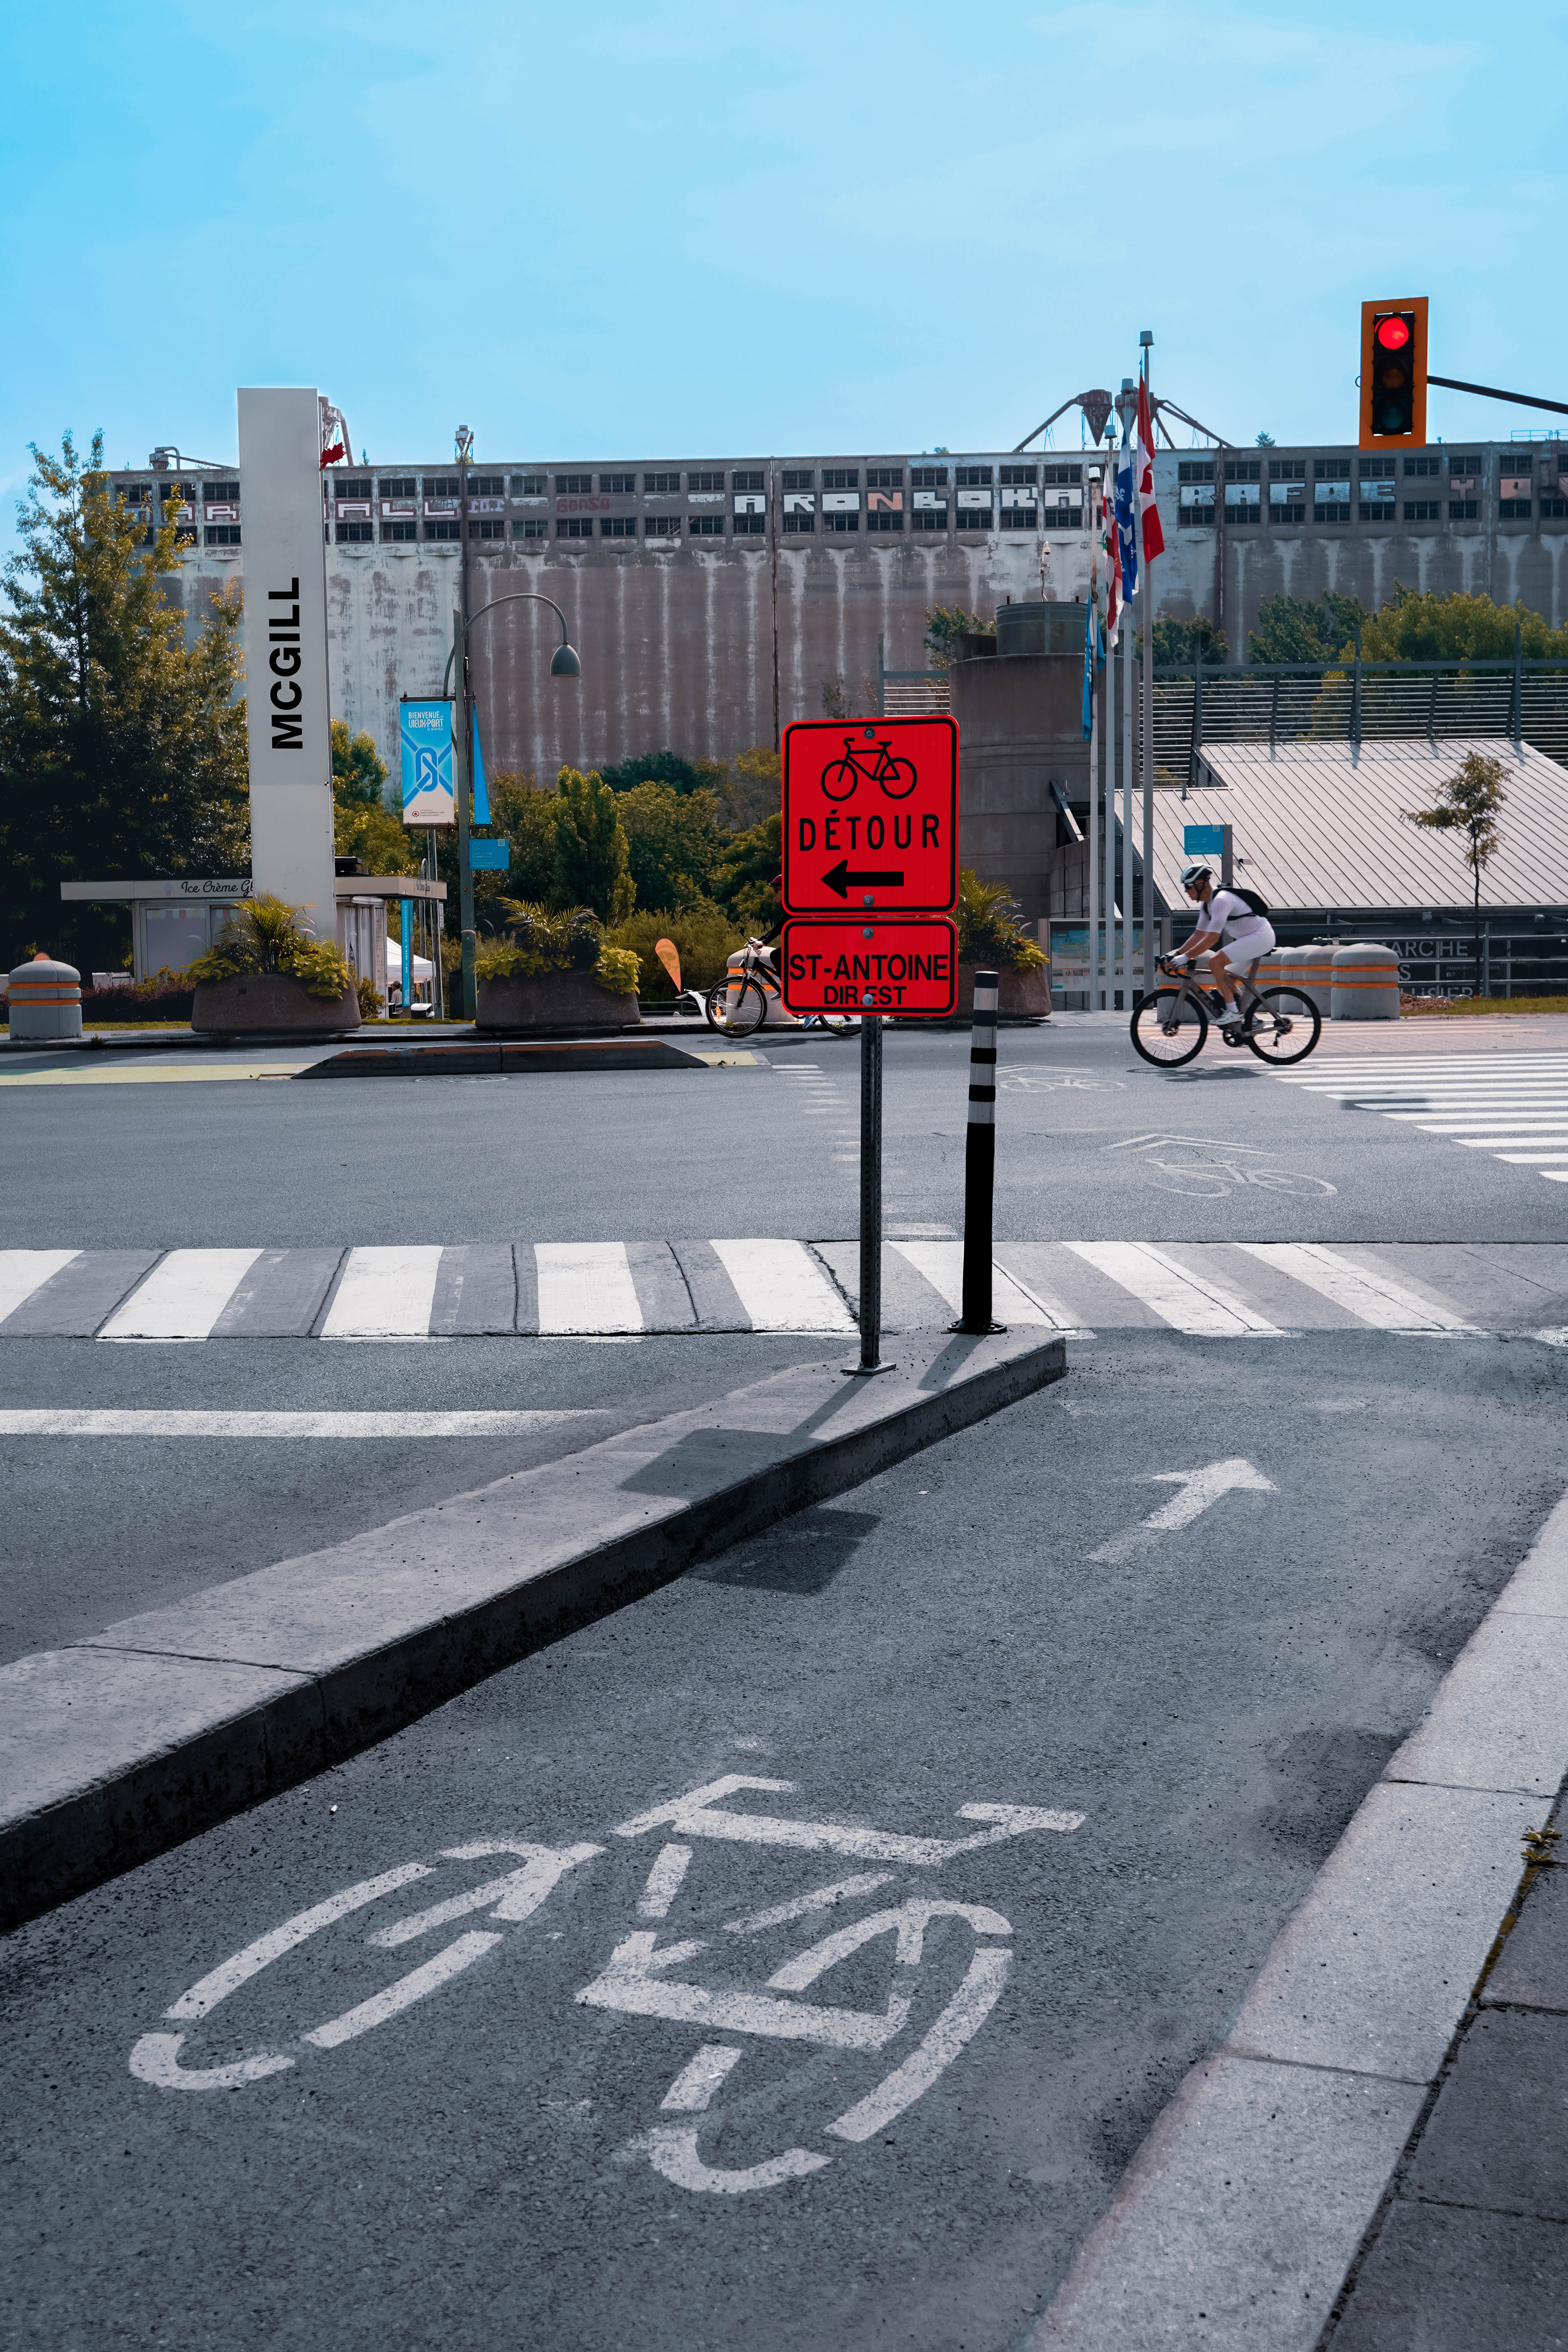
\includegraphics[width=\paperwidth,height=\paperheight]{src/Figures/Arriere_plan/Arriere_plan_Chap_5.jpg}
    }

% Rectangle
\AddToShipoutPictureBG*{
  \begin{tikzpicture}[remember picture,overlay]
    \node[fill=white, opacity=0.75, text width=\paperwidth, minimum height=9.5cm, anchor=north] 
    at ([yshift=-2cm]current page.north) {};
  \end{tikzpicture}
}

% Source
\AddToShipoutPictureFG*{
  \AtPageLowerRight{
    \raisebox{1cm}{
      \hspace{16cm}
      
\begin{tikzpicture}
        \node[fill=white, rounded corners=5pt, inner sep=5pt, align=center] {
          \tiny{Photography: \textcolor{blue}{Dylan Moinse (2022)}}
        };
      \end{tikzpicture}
    }
  }
}

    % ___________________________________________
    % Mini Table of Contents
    \cleardoublepage
    \setcounter{tocdepth}{2}
    % Redefine local table of contents title
    \renewcommand{\localcontentsname}{Table of Contents of Chapter~5}
\localtableofcontents

% Réinitialiser numérotation section
\setcounter{section}{0}

%%%%%%%%%%%%%%%%%%%%%%%%%%%%%%%%
% Chapter 2
\newpage
\section*{Key Points of Chapter~5
    \label{chap5:graphical-abstract}
    }
    \markright{Chapter Preamble}{}

\begin{figure}[h!]\vspace*{4pt}
        \caption*{}
        \label{graphical-abstract-chap2}
        \centerline{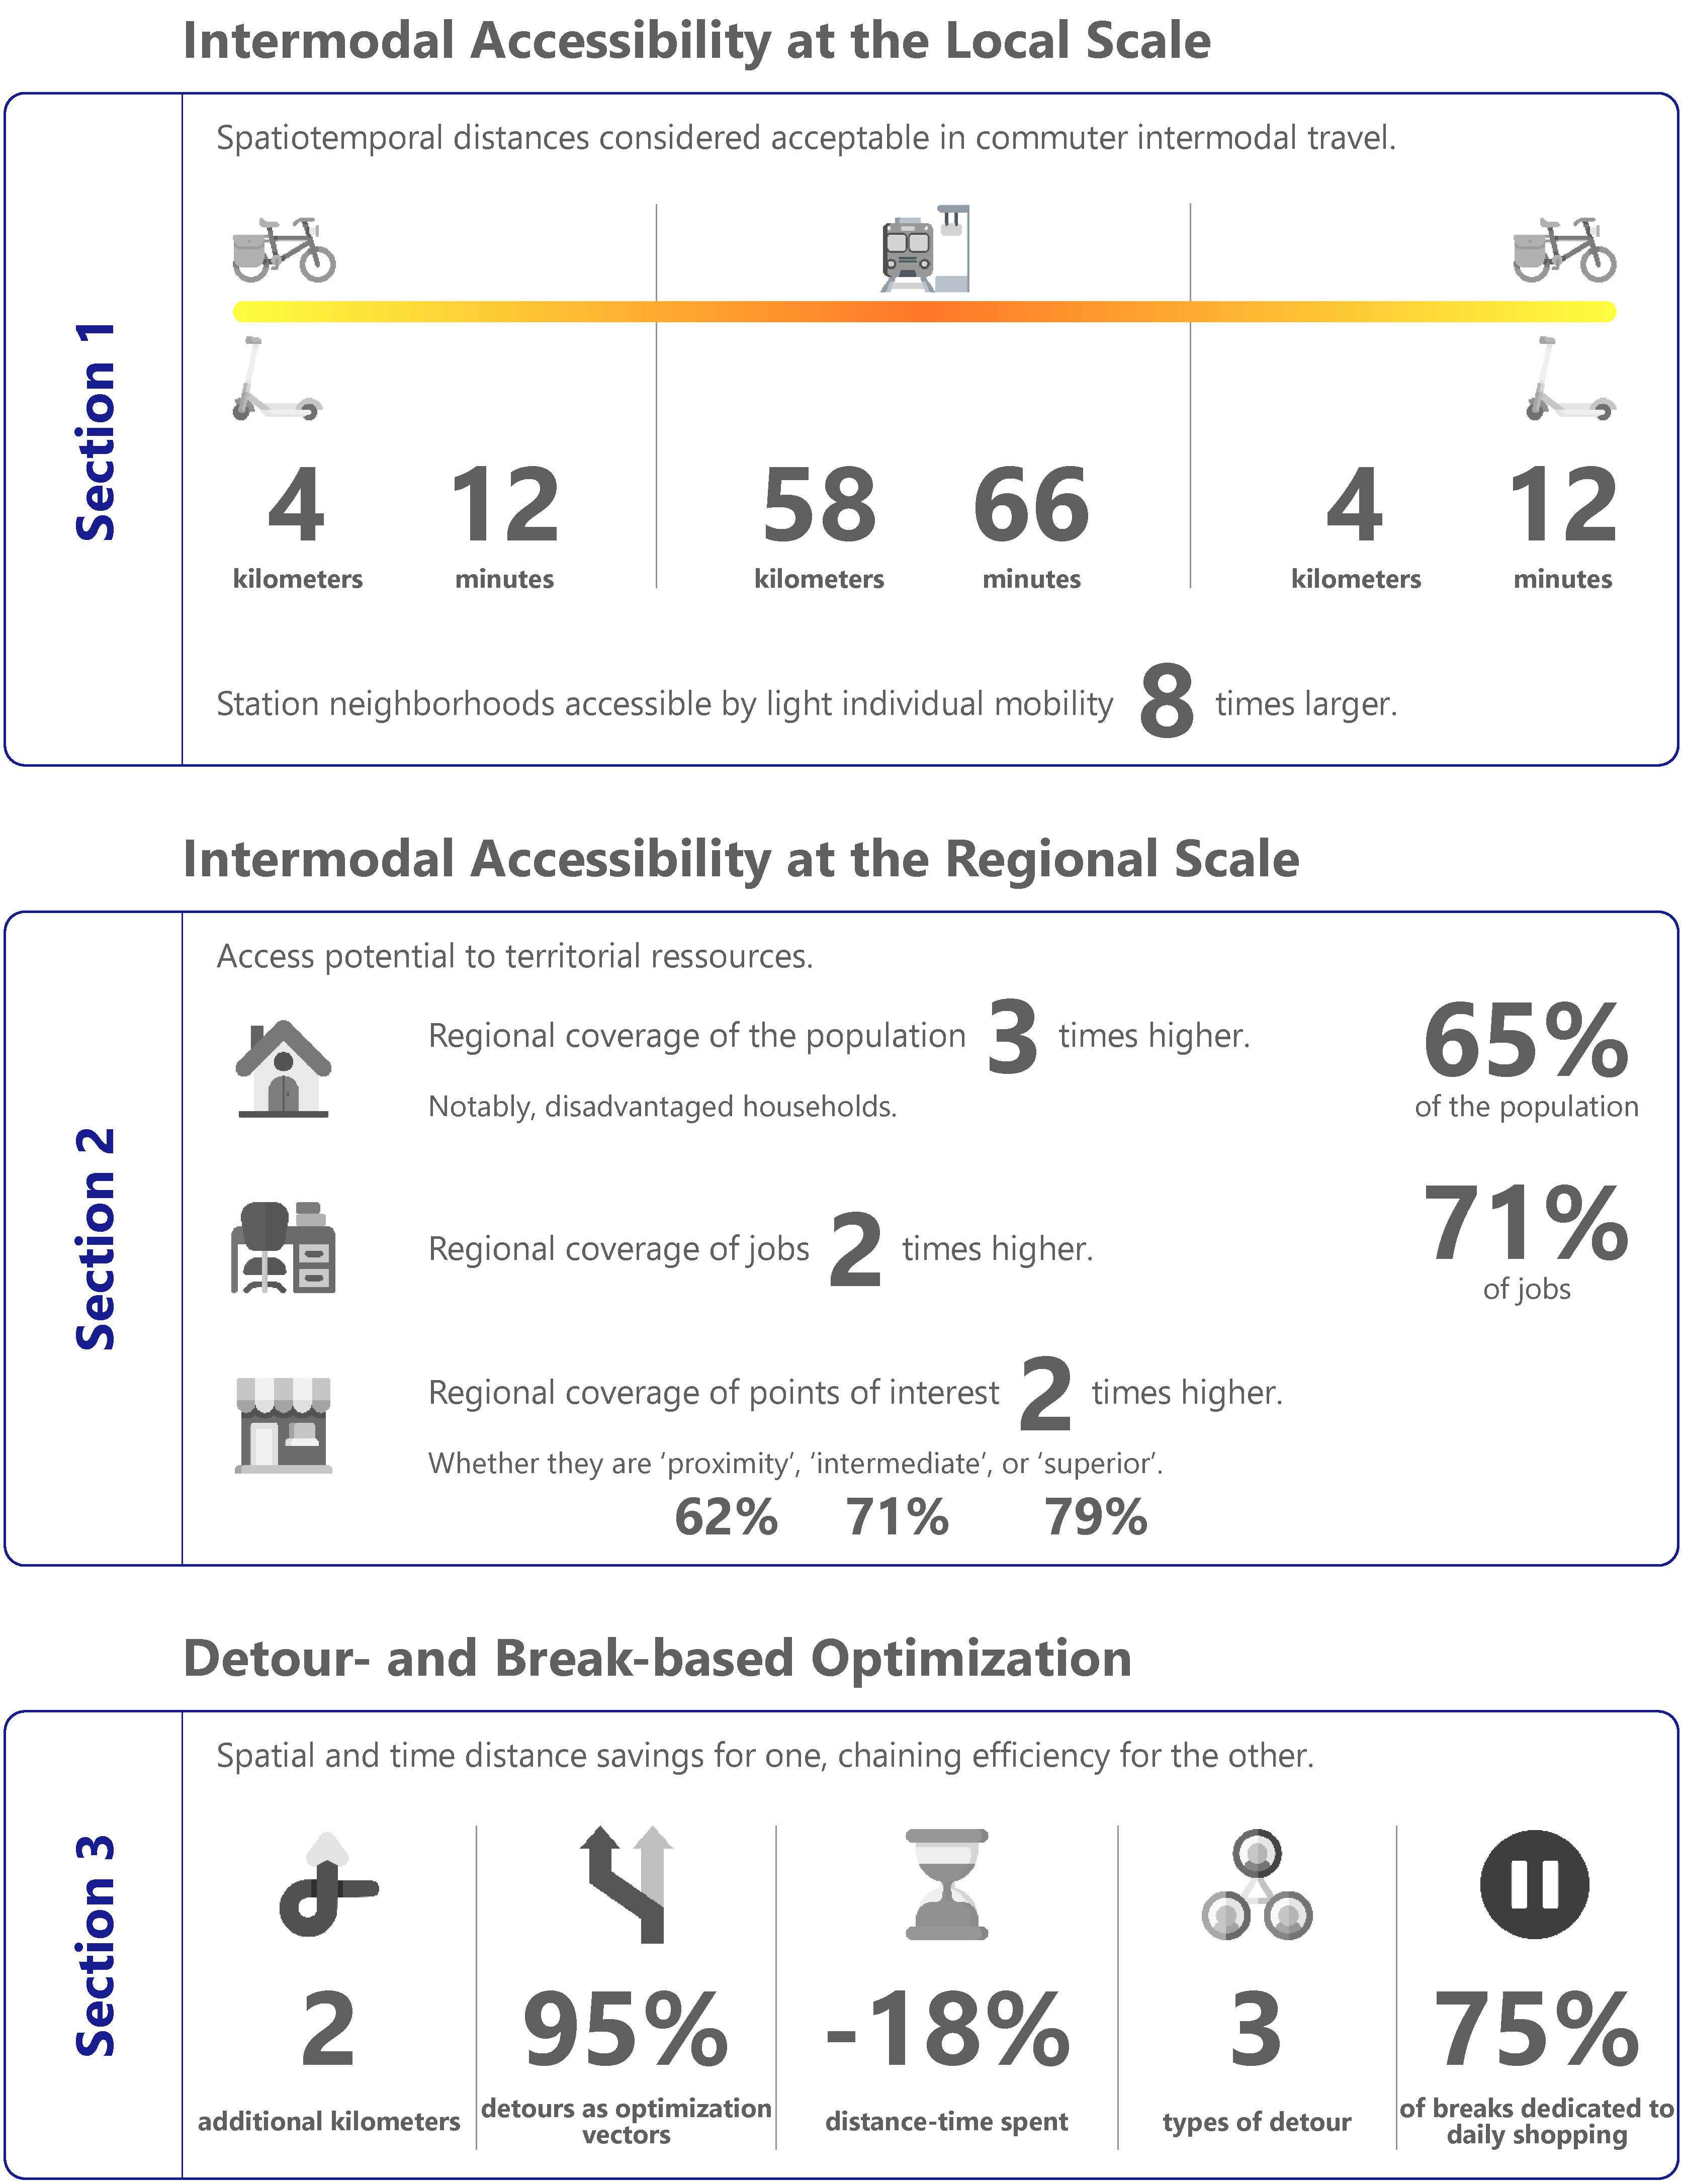
\includegraphics[width=1\columnwidth]{src/Figures/Graphical-abstract/EN_Graphical_abstract_chap5.pdf}}
        \vspace{5pt}
    \end{figure}

% ___________________________________________
% Preambule
\newpage
\begin{tcolorbox}[colback=white!5!white,
                  colframe=blue!75!blue,
                  title=
                  \bigskip
                  \center{\textbf{Preambule of Chapter~5}}
                  \\
                  \raggedright{\small{Chapter composed of \pagedifference{chap5:titre}{part2:conclusion} pages, including \pagedifference{chap5:bibliographie}{part2:conclusion} pages of bibliography}}
                  \bigskip]
\Large{\textcolor{blue}{\textbf{Abstract:}}}
    \\
    \small{
This chapter is dedicated to exploring the geographical boundaries of train station districts, examining the impact of light individual mobility, as a mode of transfer, on local and intermodal accessibility (see \hyperref[chap5:aire-cyclable-micromobilite]{Section~1}, page~\pageref{chap5:aire-cyclable-micromobilite}). Data collected from the questionnaire survey indicate that the median distance traveled by bicycle and micromobility is 2 kilometers, out of a total of 38 kilometers. Trips made for last-mile connections tend to be longer. The application of a regression model allowed for the determination of the influence of individual and contextual factors, including usage frequency, travel purpose, and the classification of socio-professional groups, as well as the variability of distances. In contrast, population density does not appear to have a significant impact on these distances.%%Translated%%
    \\
The spatial and temporal distances covered using these modes of transport are four times greater than those covered by walking, thus redefining the spatial limits around public transport hubs and multiplying the size of train station districts by eight. This spatial extension allows for the service of 7.55\% of the Hauts-de-France region in terms of isochrones, with a maximum coverage potential (buffer zones) of 18.48\%. The expanded train station districts, combining \Commas{primary areas} and \Commas{secondary areas}, serve more than half of the population and primarily provide accessibility gains to disadvantaged populations. The analysis also highlights that light individual mobility, in response to the challenge of the \Commas{first and last mile} of public transport systems, doubles the regional access potential to jobs and regional attractions. These accessibility gains illustrate the modal shift potential in favor of the rail network, particularly in areas dependent on car usage (see \hyperref[chap5:accessibilite-intermodale-extension-aire-influence]{Section~2}, page~\pageref{chap5:accessibilite-intermodale-extension-aire-influence}).%%Translated%%
    \\
The distance evaluation also explored the role of distance, and more specifically route choices, in the spatio-temporal optimization of trips, integrating detours and stops while cycling or using micromobility (see \hyperref[chap5:detours-pauses-optimisation]{Section~3}, page~\pageref{chap5:detours-pauses-optimisation}). This approach led to the identification of three optimization strategies through detours, as well as a typology of stops based on stated motives. The interactions between detours, stops, and optimization highlighted time-distance savings.%%Translated%%
    \\
This study thus sheds light on the comparative advantages and challenges of integrating light individual mobility into the rail network (see \hyperref[chap5:conclusion]{Conclusion of the Chapter}, page~\pageref{chap5:conclusion}), documenting not only the gains in regional reach and accessibility recorded by these intermodal practices, but also the flexibility of these modes of transfer, conducive to optimizing the distances traveled in the intermodal chain.%%Translated%%
    }
    \tcblower
\Large{\textcolor{blue}{\textbf{Keywords:}}}
    \\
    \small{
Accessibility;
Detour;
Distance;
Optimization;
Stop;
Public transport system performance;
Access potential;
First and last mile;
Timeliness
    }
\end{tcolorbox}

% ___________________________________________
% 5.*.
\newpage
\needspace{1\baselineskip} % Reserve space
\addcontentsline{toc}{section}{Introduction of Chapter~5}
\sectionheader{Introduction of Chapter~5}
\section*{Introduction of Chapter~5
    \label{chap5:introduction}
    }
    \markright{Introduction of Chapter~5}{}

    % Citation
    \begin{displayquote}
\Commas{[\dots] \textsl{What do social actors do when faced with geographical space, what do they \Commas{produce} through and for their spatial experience? This led us to uncover the complexity of the technologies employed by each social actor to arrange, in the context of action, a configuration where they can maintain the right distance and position themselves properly. This play of distances and positions, along with the ceaseless activity of delimiting, dividing, and evaluating sizes and metrics that always accompanies it, collectively forms, on a daily basis, nothing less than the living space of individuals in society.}}\footnote{~
    \Commas{[\dots] \textsl{que font les acteurs sociaux à l'épreuve de l'espace géographique, que \Commas{produisent}~-ils par et pour leur expérience spatiale? Cela nous a fait découvrir la complexité des technologies mises en œuvre par chaque opérateur social pour arranger, en situation d'action, une configuration où il peut se tenir à bonne distance et en bonne(s) place(s). Ce jeu des distances et des places et l'activité inlassable de délimitation, de découpage, d'évaluation des tailles et des métriques qui l'accompagne toujours, composent, au jour le jour, rien de moins que l'espace de vie des individus en société}.} \textcolor{blue}{\autocite[347]{lussault_homme_2007}}\index{Lussault, Michel|pagebf}
}

\textcolor{blue}{Michel} \textcolor{blue}{\textcite[347]{lussault_homme_2007}}\index{Lussault, Michel|pagebf}. \textsl{L’Homme spatial: La construction sociale de l’espace humain}. SEUIL, Paris, 400~p. ISBN: \href{https://search.worldcat.org/fr/title/300390192}{978-2-02-093795-5}
    \end{displayquote}

% Introduction
\lettrine[lines=3, findent=8pt, nindent=0pt]{\lettrinefont T}{his} chapter explores the spatial implications of integrating light individual mobility within public transport networks, analyzed at both local and regional scales. These modes of transfer, viewed as an efficient response to the challenge of the \Commas{first and last miles} of public transport systems, are questioned in terms of their ability to extend the geographical scope of \acrfull{TOD}. To address this general hypothesis, throughout this chapter we maintain a focus on the concept of \gls{accessibility}, specifically focusing on the local and intermodal accessibility gains associated with these intermodal practices. In this regard, we refer to the paradigm shift advocated by \textcolor{blue}{David} \textcolor{blue}{\textcite[75]{banister_sustainable_2008}}\index{Banister, David|pagebf}—through an article titled \textsl{The Sustainable Mobility Paradigm} published in the scientific journal \textsl{Transport Policy}—which posits that the \acrshort{TOD} model represents a transition from a traditional mobility conception (\textsl{planning for mobility}) to an urban planning approach centered on accessibility (\textsl{planning for accessibility}). Building on this investigation, we aim to explore various aspects that will allow for a better understanding of the expected accessibility gains, through the formulation of research objectives dedicated to this chapter, focusing on the distances and routes \Commas{produced} by \Commas{social actors} \textcolor{blue}{\autocite[347]{lussault_homme_2007}}\index{Lussault, Michel|pagebf} as well as regional accessibility.%%Translated%%

% Research Objectives
Several research objectives structure this chapter of the thesis:
\begin{customitemize}
    \item \textsl{Measure the extension of train station neighborhoods, at the local scale}. The study on the routes taken by intermodal travelers aims to measure the accessibility gains around public transport hubs, differentiating the various vehicles involved in light individual mobility, in order to identify the factors influencing the distances traveled and to determine the extent of pedestrian and cycling train station neighborhoods;
    \item \textsl{Evaluate accessibility gains, at the regional scale}. The objective is to compare the regional coverage of train station neighborhoods by considering the combined reach of walking and light individual mobility. This analysis specifically focuses on quantifying the population's potential access to public transport infrastructure, housing types, jobs, and regional amenities;
    \item \textsl{Examine the route choices of users} combining light individual mobility and the public transport network, focusing on detours and breaks.
\end{customitemize}%%Translated%%

% Plan Announcement 1
We will first conduct a statistical analysis of the spatial and temporal distances characterizing the intermodal trips collected through the online questionnaire, ensuring to distinguish the various segments that make up each \gls{journey} (\hyperref[chap5:aire-secondaire-quartier-gare]{Section~1}, page~\pageref{chap5:aire-secondaire-quartier-gare}). This section will address the delineation of the \Commas{secondary area} of \acrshort{TOD} neighborhoods based on the individual distances measured (\hyperref[chap5:aire-cyclable-micromobilite]{Subsection~1.1}, page~\pageref{chap5:aire-cyclable-micromobilite}) and will examine the individual and contextual characteristics influencing the measured distances, through statistical modeling (\hyperref[chap5:regression-distances]{Subsection~1.2}, page~\pageref{chap5:regression-distances}).%%Translated%%

% Plan Announcement 2
Following the determination of the size of train station neighborhoods based on criteria for acceptable spatial and temporal distances, we will evaluate the impact of these accessibility gains at the regional scale of Hauts-de-France (\hyperref[chap5:accessibilite-intermodale-extension-aire-influence]{Section~2}, page~\pageref{chap5:accessibilite-intermodale-extension-aire-influence}). We will focus on the potential for modal shift in favor of the railway system, examining the service provision to the population and the social inclusivity of this intermodal accessibility (\hyperref[chap5:couverture-population]{Subsection~2.1}, page~\pageref{chap5:couverture-population}), as well as the opportunities for access to regional points of attraction (\hyperref[chap5:couverture-population]{Subsection~2.2}, page~\pageref{chap5:accessibilite-emplois}).%%Translated%%

% Plan Announcement 3
The final phase of this chapter will focus on the study of route choices, directing our attention to a subset of bicycle or micromobility trips around public transport stations. The aim of \hyperref[chap5:detours-pauses-optimisation]{Section~3} (page~\pageref{chap5:detours-pauses-optimisation}) is to shed light on the motivations behind such detours and intermediate stops. To this end, we will explore the existing link in the scientific literature between detours, breaks, and the optimization of movement (\hyperref[chap5:enjeux-detours-pauses]{Subsection~3.1}, page~\pageref{chap5:enjeux-detours-pauses}). We will then present our statistical analysis method (\hyperref[chap5:methodes-statistiques]{Subsection~3.2}, page~\pageref{chap5:methodes-statistiques}) designed to verify whether these detours and breaks contribute to distance-time gains (\hyperref[chap5:strategies-optimisation]{Subsection~3.3}, page~\pageref{chap5:strategies-optimisation}), before discussing these findings (\hyperref[chap5:discussion-detours-pauses-optimisation]{Subsection~3.4}, page~\pageref{chap5:discussion-detours-pauses-optimisation}).%%Translated%%

% Plan Announcement 4
In conclusion, we will summarize the key findings of this chapter, which provide insights into the extension of train station neighborhoods and their spatial implications within the regional perimeter (\hyperref[chap5:conclusion]{Conclusion of Chapter~5}, page~\pageref{chap5:conclusion}).%%Translated%%

% ___________________________________________
% 5.1.
\newpage
\needspace{1\baselineskip} % Reserve space
\sectionheader{Determination of a Secondary Area}
\section{Measurement of the \Commas{Secondary Area} around the Railway Station Area and the Potential for Intermodal Use by Cyclists
    \label{chap5:aire-secondaire-quartier-gare}
    }

% Introduction
In this first section, we aim to explore how the spatiotemporal distances considered acceptable by \gls{bicycle} and \gls{micromobility}, as modes of transfer to and from public transport networks, can define the extension of railway station districts. By analyzing home-to-work and home-to-study trips, we are able to determine the effective reach of these modes of transport and thus infer their capacity to expand the influence area, referred to as the \Commas{secondary area,} of train stations in the Hauts-de-France region. Based on the responses gathered through the survey conducted with intermodal users, this study first seeks to quantify the distribution of travel distances, as detailed in the \hyperref[chap5:aire-cyclable-micromobilite]{first subsection defining the extension of railway station districts} (page~\pageref{chap5:aire-cyclable-micromobilite}). Secondly, it reveals, through the \hyperref[chap5:regression-distances]{second subsection modeling the factors influencing distance} (page~\pageref{chap5:regression-distances}), the variation in distances based on various factors related to mobility behaviors, the urban environment, and socio-demographic characteristics.%%Translated%%

% 5.1.1.
\needspace{1\baselineskip} % Reserve space
\subsection{Measurement of the Acceptable Cycling Area around Public Transport Hubs
    \label{chap5:aire-cyclable-micromobilite}
    }

% Introduction
Our primary objective is to measure the relevance area of light individual mobility around public transport hubs. Based on the distance analysis from the responses of the users who participated in our survey, we have mapped and studied the distribution of the spatial distances traveled for each segment of their commuting trips. The following descriptive statistics are thus based on 217 responses and 262 trips by bike or micromobility, which allowed us to determine the effective reach of these modes of transport and, consequently, to define the boundaries of an extended \acrshort{TOD} district.%%Translated%%

% 5.1.1.1.
\needspace{1\baselineskip} % Reserve space
\subsubsection*{Spatial Distances Traveled Using Light Individual Mobility
    \label{chap5:distances-spatiales-parcourues}
    }

% Figure violons distances
\begin{figure}[h!]\vspace*{4pt}
    \caption{Violin plots of access and egress distances traveled by intermodal commuters using light individual mobility.}
    \label{fig-chap5:diagrammes-violons}
    \centerline{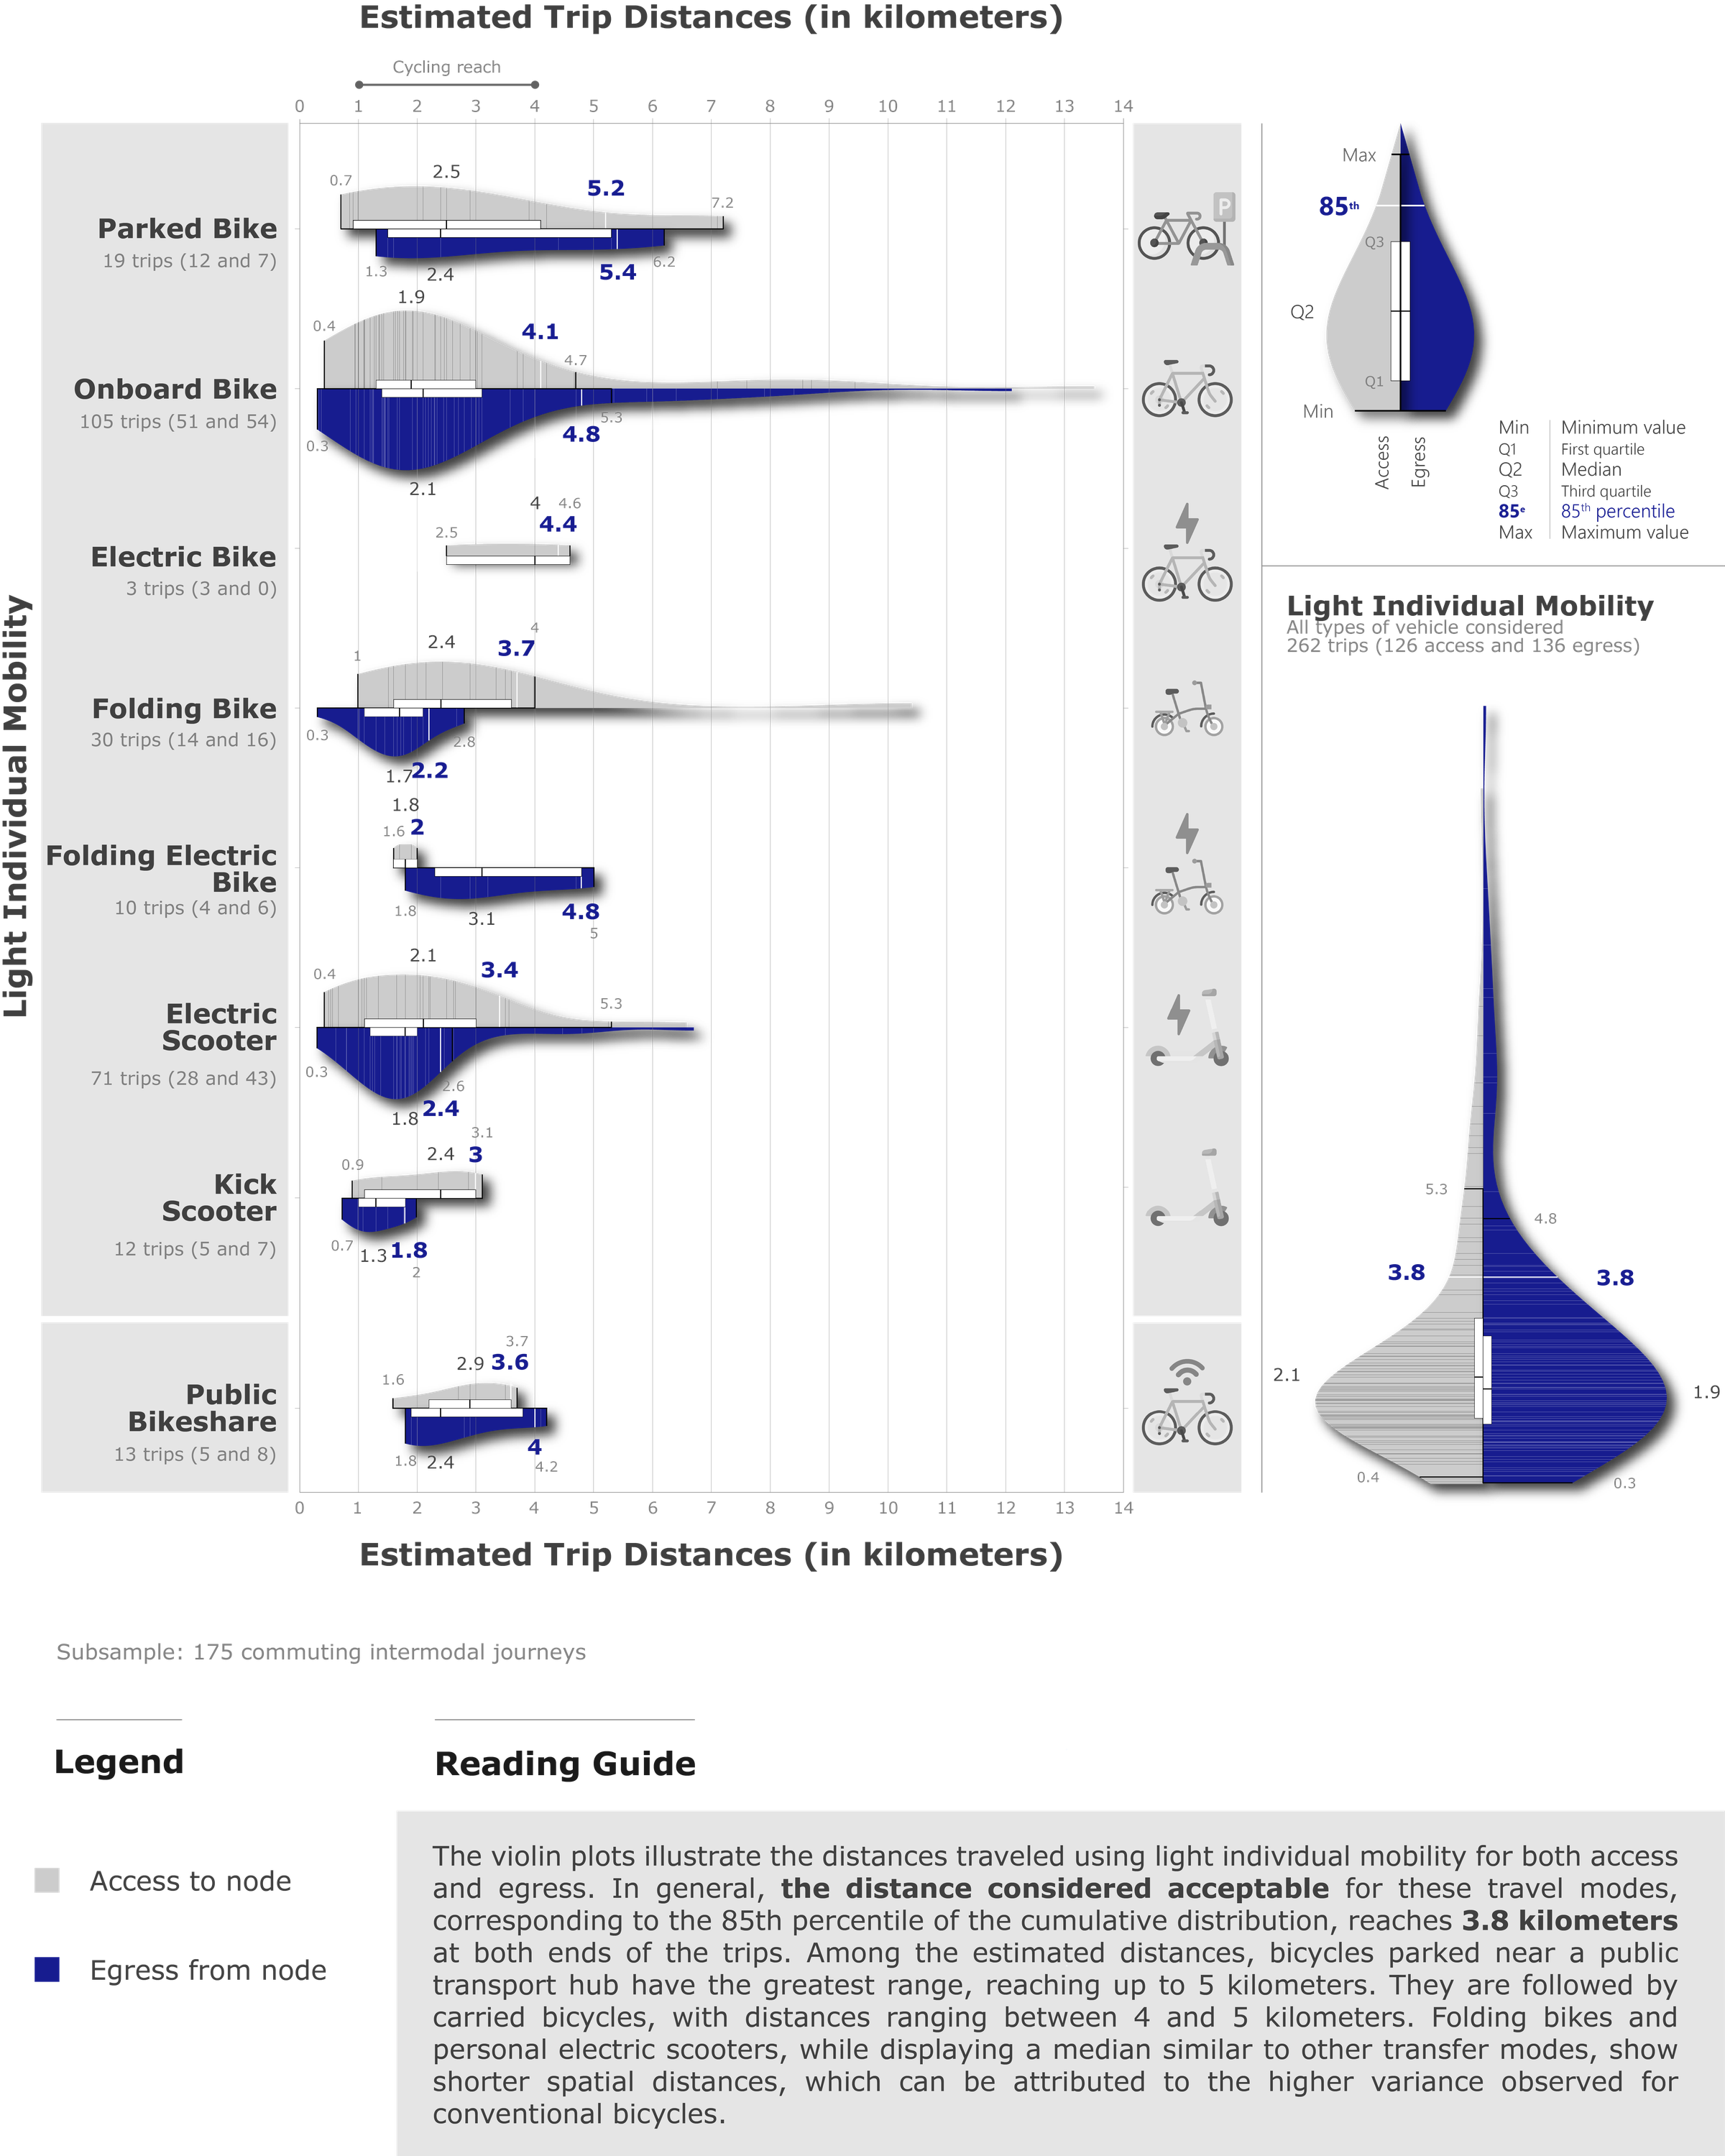
\includegraphics[width=1\columnwidth]{src/Figures/Chap-5/EN_Distances_Violons_Navetteurs.png}}
    \vspace{5pt}
    \begin{flushright}\scriptsize{
    Author: \textcolor{blue}{Dylan Moinse (2023)}
    }\end{flushright}
\end{figure}

% Statistiques distances parcourues
The examination of the distances involved in home-to-work commutes using light individual mobility, both for the access and egress stages, reveals the adoption of a relevant geographic perimeter around public transport hubs, extending three to four kilometers in each direction. More specifically, the median distance traveled by bike or micromobility is 2 kilometers, broken down into 2.1 kilometers for the access trip and 1.9 kilometers for the egress segment. However, it should be noted that the distance considered acceptable, which defines the reach of these modes of transport, is more accurately derived from the 85\textsuperscript{th} percentile of the cumulative distribution of traveled distances, as introduced in the \hyperref[chap3:quartiers-gare-distances]{section dedicated to the spatialization of station districts} (page~\pageref{chap3:quartiers-gare-distances}) of \hyperref[chap3:titre]{chapter~3} (page~\pageref{chap3:titre}). Based on this measure, the critical distance for light individual mobility, for both the first and last kilometers, is estimated at 3.8 kilometers for each \gls{itinerary} (see \hyperref[fig-chap5:diagrammes-violons]{illustration~\ref{fig-chap5:diagrammes-violons}}, page~\pageref{fig-chap5:diagrammes-violons}). Consequently, the range around station districts, adapted to cycling and micromobility, reaches 3.8 kilometers, compared to only 1.3 kilometers when measured for walking. It is also worth noting that minor variations are observed between the distances traveled in the two scenarios studied: The access trip from home generally shows longer distances, ranging from 0.4 to 5.3 kilometers, while the distances for segments towards the activity location range from 0.3 to 4.8 kilometers.%%Translated%%

% Distances selon le type de MIL
Considering all trips with a utilitarian purpose or for leisure, our analysis relied on the representation of the impedance function\footnote{~
    The impedance function can be used in transport modeling to express how the friction of spatial or temporal distance influences the probability or quantity of trips. It is based on the assumption that individuals do not stop traveling instantly after a certain spatiotemporal distance, but that their probability of traveling decreases gradually. It is a decreasing function that quantifies the reduction in the number of trips with the increase in travel cost. In their scientific article titled \foreignlanguage{english}{\textsl{The Influence of the Impedance Function on Gravity-based Pedestrian Accessibility Measures: A Comparative Analysis}}, \textcolor{blue}{\textcite[758]{vale_influence_2017}}\index{Vale, David~S.|pagebf}\index{Pereira, Mauro|pagebf} analyzed twenty gravity-based accessibility measures by varying the impedance functions and their associated parameters. The factor analysis produced showed that the measures yield similar results for identifying the \Commas{acceptable walking distance.} Following their recommendations for spatial studies on urban accessibility, we applied the cumulative Gaussian impedance function to model the perception of distances in intermodal trips.
}, associated with the quantification of the costs involved in a trip. This model primarily predicts modal choice and route selection based on the resistances encountered on each route option. The statistical analysis determined that making a trip using light individual mobility connected to the public transport network is relatively inexpensive for users when the spatial distance radius is between 0.8 and 4.2 kilometers for the access phase, and between 0.5 and 3.3 kilometers for the egress phase (see \hyperref[fig-chap5:impedance-distances]{Figure~\ref{fig-chap5:impedance-distances}}, page~\pageref{fig-chap5:impedance-distances}). A graphical examination of the cumulative data reveals that conventional bicycles have an acceptable range from 0.8 to 4.8 kilometers for the access and from 1.3 to 5.2 kilometers for the egress. In contrast, the impedance function for folding bicycles suggests that their range is less costly, ranging from 1.1 to 4 kilometers on one hand, and from 0.4 to 2.8 kilometers on the other hand. For the \acrfull{PeS}, the associated spatial distance intervals are respectively between 0.5 and 3 kilometers, and between 0.3 and 2.7 kilometers. Walking, in turn, corresponds to a maximized range of between 0.1 and 1.2 kilometers and between 0.2 and 1.1 kilometers. It thus appears that light individual mobility and combined walking practices are hierarchically structured according to the distance traveled. Indeed, the conventional bicycle stands out as the preferred cycling mode for longer trips that involve a certain minimum distance, followed by folding bicycles, \acrshort{PeS}, \acrfull{PBS}, and \acrfull{DBS}. Walking occupies the last position in this stratification, being mostly adopted for the shortest distances. However, it is worth noting that pedestrian trips in the egress phase, as reported in this survey, are generally preceded by the use of a regular bicycle before accessing the public transport station.%%Translated%%

% Figure fonctions d'impédance distances - fonction de décroissance
\begin{figure}[h!]\vspace*{4pt}
    \caption{Determination of the impedance of access and egress distances traveled by intermodal travelers using light individual mobility.}
    \label{fig-chap5:impedance-distances}
    \centerline{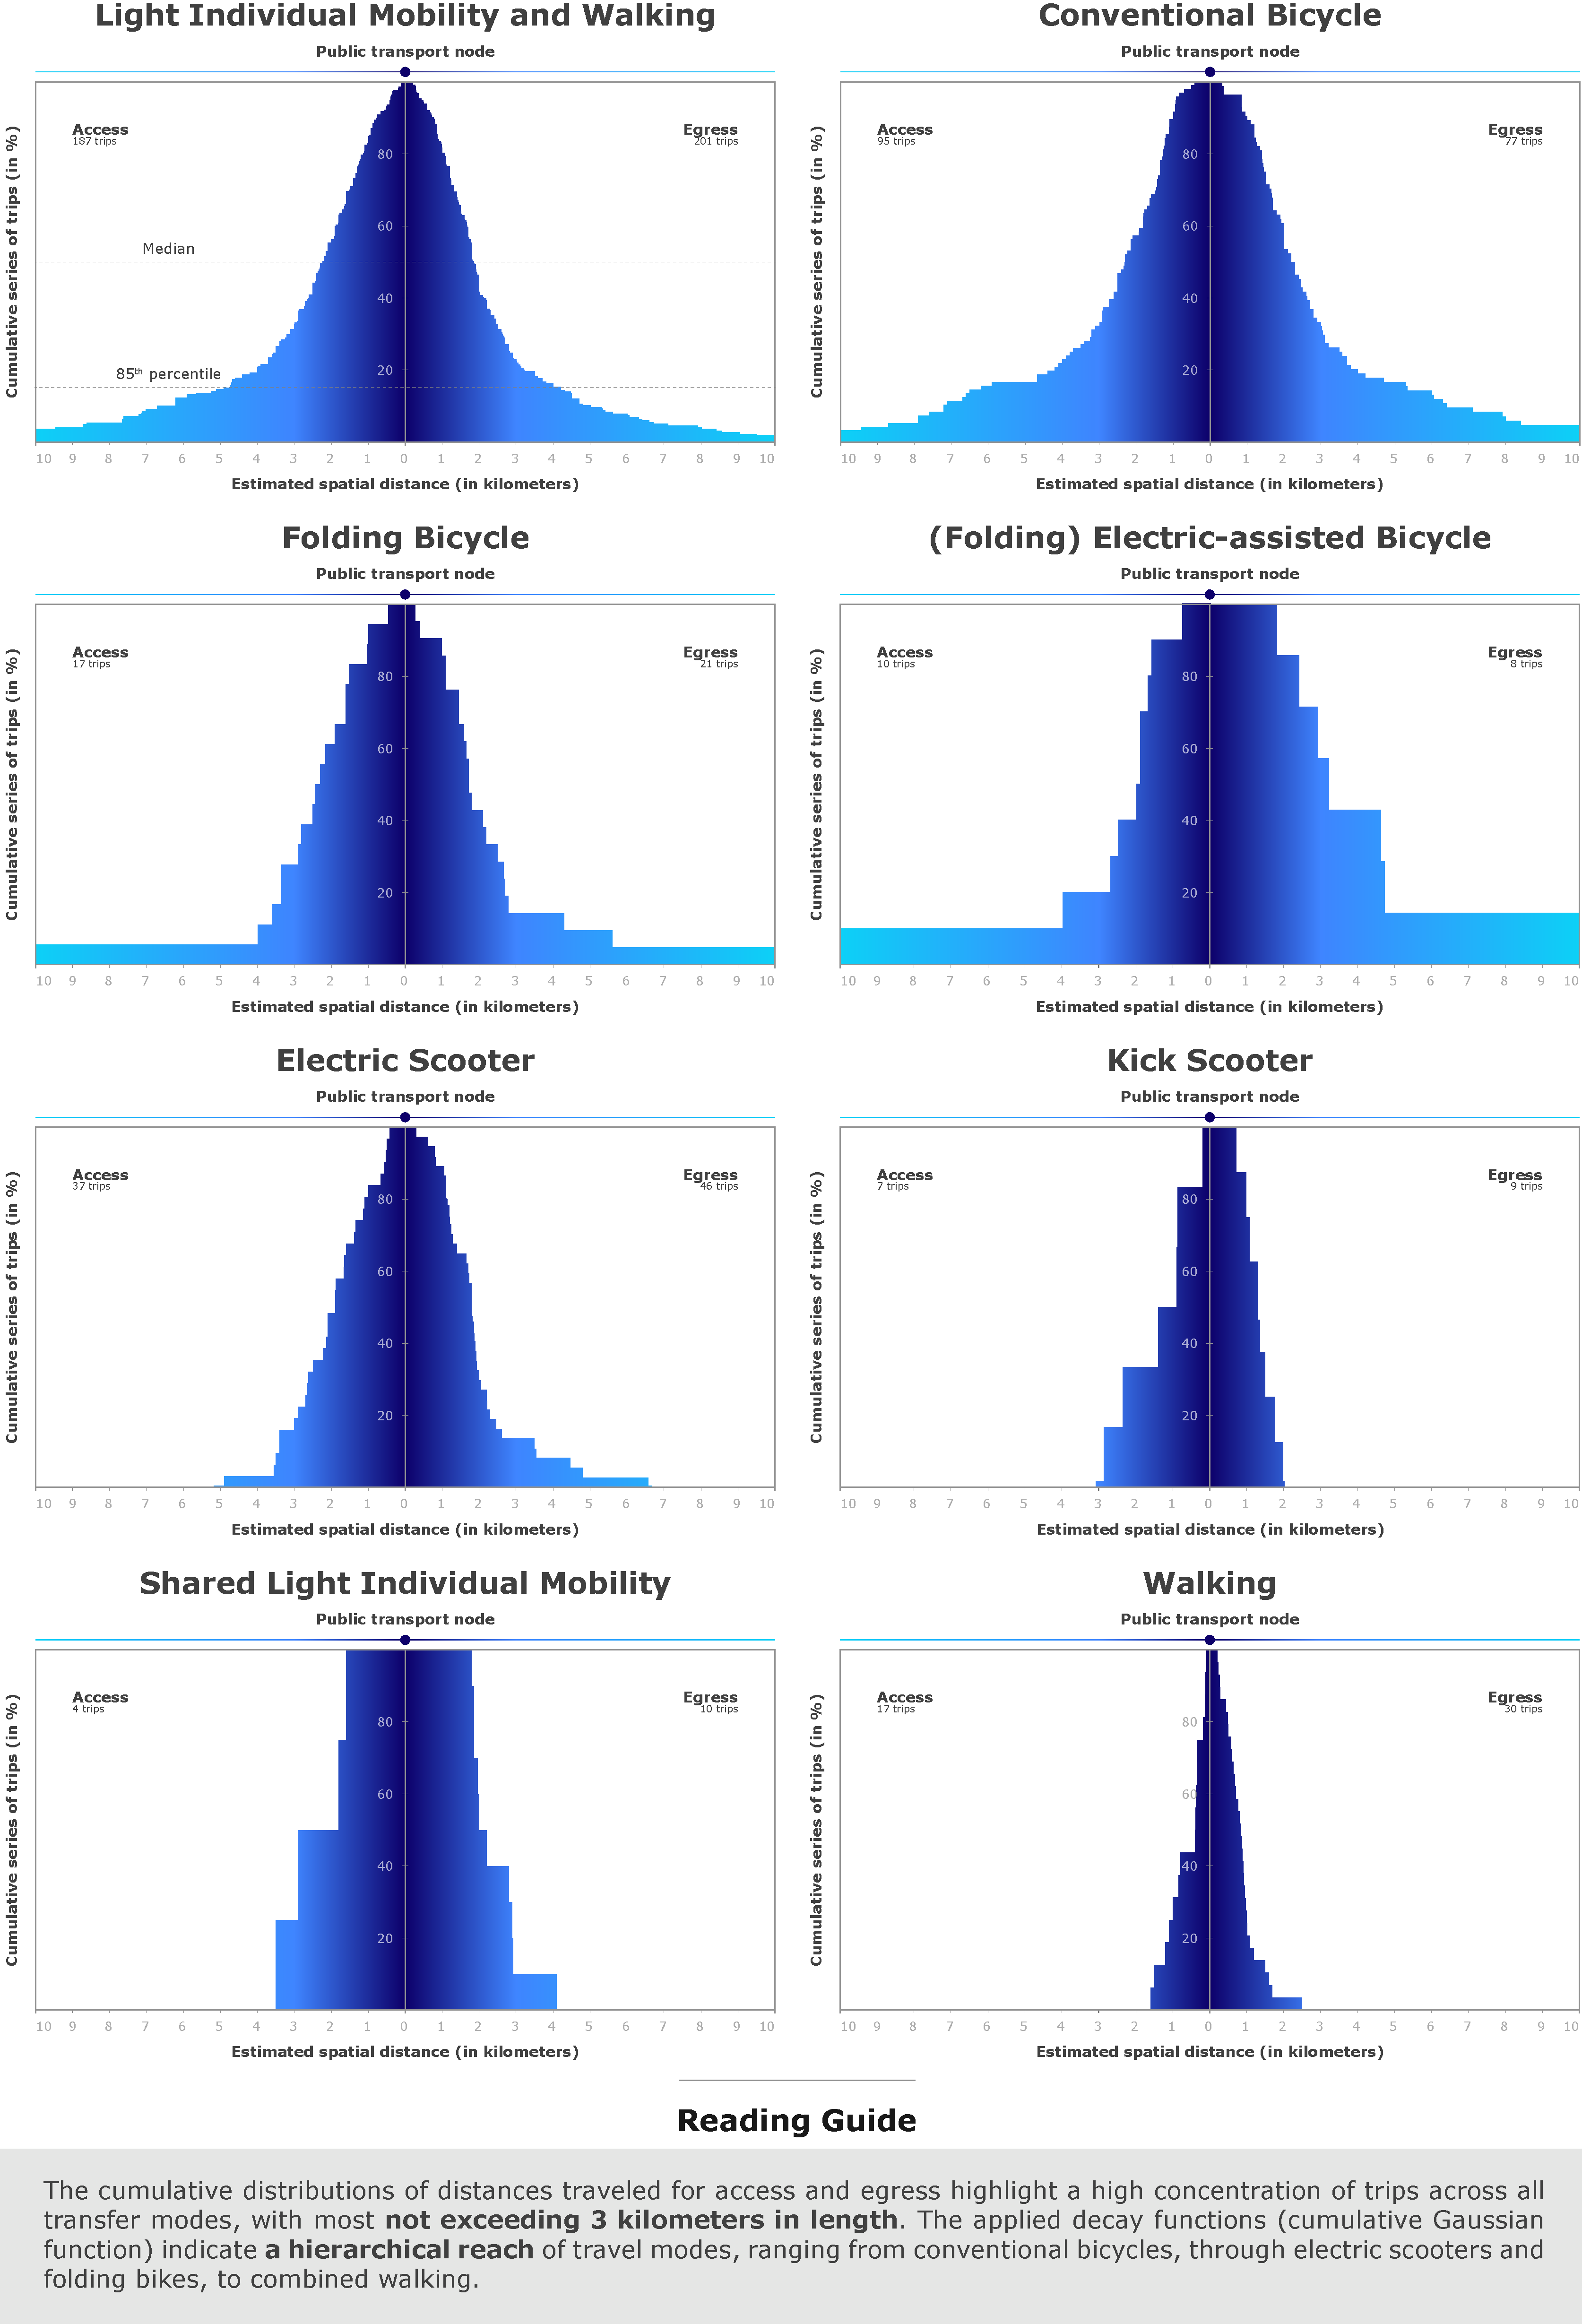
\includegraphics[width=1\columnwidth]{src/Figures/Chap-5/EN_Distances_Impedance.pdf}}
    \vspace{5pt}
    \begin{flushright}\scriptsize{
    Author: \textcolor{blue}{Dylan Moinse (2024)}
    }\end{flushright}
\end{figure}

% Symétrie de gains de distance selon l'embarquement
An additional aspect considered in this study on distances concerns the effect of asymmetry or symmetry of the accessibility benefits offered by light individual mobility. The ability to carry one's vehicle on the public transport network, or to have a second bicycle during the egress phase, allows for increased distances both in the first and last kilometers of an intermodal trip. The analysis of the modal configurations adopted during the two segments shows that, in general, 66.97\% of travelers use the same mode of transport during both phases. This phenomenon is particularly prevalent among folding bicycle users (82.61\%) and \acrshort{PeS} users (79.49\%). Conventional bicycles rank third, with 71.96\% of cyclists using them for both the access and egress phases.%%Translated%%

% Suite symétrie de gains de distance
This diagram illustrates a certain comparative advantage of the lightest and most easily transportable vehicles aboard collective transport modes: folding bicycles and \acrshort{PeS} provide a solution adapted to the specific issue of the \Commas{last kilometers,} effectively doubling their range on both sides of the station. We also identified such mobility practices in the Provence-Alpes-Côte d'Azur region, where 85\% of rail travelers using \acrshort{PeS} or mechanical scooters use these \acrshort{PMD} for both their first and last kilometers, compared to only 34\% of passengers overall \textcolor{blue}{\autocite[185]{moinse_intermodal_2022}}\index{Moinse, Dylan|pagebf}\index{Goudeau, Matthieu|pagebf}\index{L'Hostis, Alain|pagebf}\index{Leysens, Thomas|pagebf}.%%Translated%%

% Symétrie questionnaire parcours commentés
Further analysis of the question \Commas{\textsl{Why did you bring your vehicle with you?}} included in the survey shows that 87.22\% (157 participants) of users who chose to bring their bicycle or micro-vehicle indicated that the main motivation was the possibility of using it after leaving the station, due to distances considered too long. Additionally, 6.11\% of respondents (11 participants) cited insecure parking facilities as their reason, while 5\% (9 participants) reported the lack of nearby parking facilities. Furthermore, the main reason for bringing the \acrshort{PeS} also appears in the commented journey with participant \(PCTE_{2}\). The participant justifies the combined use of this \acrshort{PMD} with the metro to reach his two destinations in Villeneuve d'Ascq, although he acknowledges that his access leg could have been made on foot.%%Translated%%

% Distances selon le type de TC
While the range of spatial distances traveled by intermodal travelers using light individual mobility differs depending on the type of vehicle, it is also influenced by the nature of the public transport system, in line with the scientific literature \textcolor{blue}{\autocite[105]{flamm_public_2014}}\index{Flamm, Bradley~J.|pagebf}\index{Rivasplata, Charles~R.|pagebf}. Indeed, it appears that stations integrated into the \acrshort{HST} network have an influence area extending up to a radius of four kilometers, while those served only by the \acrshort{TER} or \acrshort{TERGV} networks have a radius of about three kilometers. For urban rail-based public transport systems, such as the metro and tramway, the average radius is estimated at two kilometers. Referring to the segmentation of the \acrfull{DRG} (see the \hyperref[chap4:part-modale-gares-centre-periurbain]{section dedicated to the modal share of light individual mobility in transfer at station types}, page~\pageref{chap4:part-modale-gares-centre-periurbain} of \hyperref[chap5:titre]{Chapter~5}, page~\pageref{chap5:titre}), established by \textcolor{blue}{\textcite{sncf_gares__connexions_gares_2024}}\index{SNCF Gares \& Connexions@\textsl{SNCF Gares \& Connexions}|pagebf}, which classifies French stations into different groups according to various criteria, we can observe that the distance considered acceptable by bike or micromobility, set at the 85\textsuperscript{th} percentile, decreases proportionally with the level of service at the station (see \hyperref[table-chap5:distances-type-tc]{Table~\ref{table-chap5:distances-type-tc}}, page~\pageref{table-chap5:distances-type-tc}). Thus, category \(a\) stations have an acceptable distance of 4.8 kilometers, while category \(b\) and category \(c\) stations show distances of 4.26 kilometers and 3.8 kilometers, respectively.%%Translated%%

    % Tableau distances selon TC
% Table of distances by public transport type
%%Translated%%
        \begin{table}[h!]
        \centering
        \renewcommand{\arraystretch}{1.5}
        \resizebox{\columnwidth}{!}{
        \begin{tabular}{p{0.38\columnwidth}p{0.1\columnwidth}p{0.12\columnwidth}p{0.1\columnwidth}p{0.1\columnwidth}p{0.1\columnwidth}p{0.1\columnwidth}}
        %\hline
    \rule{0pt}{15pt} \multirow{1.5}{*}{\small{\textbf{\textcolor{blue}{Typology}}}} & \small{\textbf{\textcolor{blue}{25\textsuperscript{th} percentile}}} & \multirow{1.5}{*}{\small{\textbf{\textcolor{blue}{Median}}}} & \small{\textbf{\textcolor{blue}{85\textsuperscript{th} percentile}}} & \multirow{1.5}{*}{\small{\textbf{\textcolor{blue}{Min.}}}} &  \multirow{1.5}{*}{\small{\textbf{\textcolor{blue}{Max.}}}} &  \multirow{1.5}{*}{\textbf{\textcolor{blue}{$\sigma$}}}\\
        \hline
\small{All types of network combined} & \multirow{1.5}{*}{\small{1.30}} & \multirow{1.5}{*}{\small{2.00}} & \multirow{1.5}{*}{\small{\textbf{3.80}}} & \multirow{1.5}{*}{\small{0.20}} & \multirow{1.5}{*}{\small{54.60}} & \multirow{1.5}{*}{\small{15.12}}\\
        \hdashline
\small{Category \(a\) stations} & \small{1.70} & \small{2.40} & \small{\textbf{4.80}} & \small{0.37} & \small{54.60} & \small{24.38}\\
\small{Category \(b\) stations} & \small{1.42} & \small{1.94} & \small{\textbf{4.26}} & \small{0.21} & \small{39.90} & \small{4.90}\\
\small{Category \(c\) stations} & \small{1.33} & \small{1.66} & \small{\textbf{3.80}} & \small{0.78} & \small{46.10} & \small{10.23}\\
\small{Metro and tram stops} & \multirow{1.5}{*}{\small{0.67}} & \multirow{1.5}{*}{\small{1.05}} & \multirow{1.5}{*}{\small{\textbf{2.37}}} & \multirow{1.5}{*}{\small{0.20}} & \multirow{1.5}{*}{\small{9.10}} & \multirow{1.5}{*}{\small{1.84}}\\
        \hline
        \end{tabular}}
    \caption{Distribution of spatial distances covered for last-mile connections or diffusion in commuting journeys, based on the type of public transport system and station category.}
    \label{table-chap5:distances-type-tc}
        \vspace{5pt}
        \begin{flushleft}\scriptsize{
        \textcolor{blue}{Note:} $\sigma$ corresponds to the standard deviation.
        \\
        \textcolor{blue}{Reading Guide:} The spatial distances covered for last-mile connections or diffusion vary significantly depending on the type of station and network: category \(a\) stations record the highest distances, while urban rail stops display notably shorter distances.
        }\end{flushleft}
        \begin{flushright}\scriptsize
        Author: \textcolor{blue}{Dylan Moinse (2023)}
        \end{flushright}
        \end{table}%%Rédigé%%

% Littérature
When comparing the distances estimated in our study with those reported in the scientific literature, it appears that our findings align with previously established results concerning intermodal practices. Indeed, the geographical relevance area around stations, estimated to be between three and four kilometers, is validated by the work of \textcolor{blue}{\textcite[234]{keijer_how_2000}}\index{Keijer, Majanka|pagebf}\index{Rietveld, Piet|pagebf}, \textcolor{blue}{\textcite[359]{givoni_access_2007}}\index{Givoni, Moshe|pagebf}\index{Rietveld, Piet|pagebf}, \textcolor{blue}{\textcite[23]{debrezion_modelling_2009}}\index{Debrezion, Ghebreegziabiher|pagebf}\index{Pels, Eric|pagebf}\index{Rietveld, Piet|pagebf}, \textcolor{blue}{\textcite[213]{kager_characterisation_2016}}\index{Kager, Roland|pagebf}\index{Bertolini, Luca|pagebf}\index{te Brömmelstroet, Marco|pagebf}, and \textcolor{blue}{\textcite[42]{nielsen_bikeability_2018}}\index{Nielsen, Thomas Alexander Sick|pagebf}\index{Skov-Petersen, Hans|pagebf}. More specifically, our impedance analysis revealed spatial distance radii where light individual mobility presents relatively low costs, ranging from 0.8 to 4.2 kilometers for the access trip, corresponding to the observations of \textcolor{blue}{Karel} \textcolor{blue}{\textcite[282]{martens_bicycle_2004}}\index{Martens, Karel|pagebf}, who reports radii ranging from 1.1 to 4.2 kilometers for the access phase, in Germany, the Netherlands, and the United Kingdom, and \textcolor{blue}{Christian} \textcolor{blue}{\textcite[14]{gioria_etude_2016}}\index{Gioria, Christian|pagebf}, who deduces a maximum distance of 5 kilometers for both access and egress using the bicycle in France. Furthermore, \textcolor{blue}{Piet} \textcolor{blue}{\textcite[73]{rietveld_accessibility_2000}}\index{Rietveld, Piet|pagebf} highlights the existence of asymmetry between the ends of an intermodal trip, with the segment from home being more likely to use a bicycle, with distances ranging from 1.2 to 3.7 kilometers. This asymmetry is also reflected in our statistical results. Regarding the concept of social acceptability of maximum distances, based on a threshold set at the 85\textsuperscript{th} percentile, our estimate of 3.8 kilometers coincides with the distances considered acceptable at 3.6 kilometers, as mentioned by \textcolor{blue}{\textcite[62]{rabaud_quand_2022}}\index{Rabaud, Mathieu|pagebf}\index{Richer, Cyprien|pagebf} and \textcolor{blue}{\textcite[45]{la_paix_puello_modelling_2015}}\index{La Paix Puello, Lissy|pagebf}\index{Geurs, Karst~T.|pagebf}. Concerning the minimum distances in favor of using the bicycle or micromobility, our conclusions align with those of \textcolor{blue}{\textcite[2]{rastogi_willingness_2010}}\index{Rastogi, Rajat|pagebf}\index{Krishna Rao,~K.~V.|pagebf}, for whom the bicycle becomes a competitive alternative to walking combined with distances starting at 1.3 kilometers around stations. It should be noted that the measured spatial distances are, however, smaller than the acceptable radius for the monomodal use of bicycles in the Hauts-de-France region, at 5.6 kilometers \textcolor{blue}{\autocite[20]{hasiak_estimation_2023}}\index{Hasiak, Fabrice|pagebf}\index{Verdier, Laurent|pagebf}.%%Translated%%

% 5.1.1.2.
\needspace{1\baselineskip} % Reserve space
\subsubsection*{Distance-Time Traveled Using Light Individual Mobility
    \label{chap5:distances-temps-parcourues}
    }

% Distance-temps globale
When examining the average duration of trips associated with the \Commas{first and last kilometers,} across all modes of transport—including walking, light individual mobility, car use as a driver or passenger, as well as urban public transport systems—the average duration of an access trip is 13 minutes and 20 seconds (218 trips), while the egress trip duration reaches 18 minutes and 51 seconds (218 trips). Combining both types of segments in the travel chain, the average trip duration is 16 minutes and 5 seconds (436 trips).%%Translated%%
  
% Distance-temps mobilité individuelle légère
Focusing specifically on light individual mobility, the estimated average duration of access trips is 11 minutes and 37 seconds (173 trips), and increases to 20 minutes and 11 seconds (181 trips) for the egress phase. This contrast between the two segments, while the overall average trip duration is 16 minutes for 354 trips, can be attributed to particularly long trips made when leaving the public transport station, especially by electric bicycle. Excluding walks, classified as \Commas{undirected trips} by \textcolor{blue}{\textcite[8-9]{hook_undirected_2021}}\index{Hook, Hannah|pagebf}\index{Vos, Jonas de|pagebf}\index{Acker, Veronique van|pagebf}\index{Witlox, Frank|pagebf}, the average distance-time for trips from home is reduced to 11 minutes and 43 seconds, and 13 minutes and 51 seconds towards the activity location, with an overall duration for light individual mobility trips of 12 minutes and 45 seconds.%%Translated%%

% Distance-temps autres modes de transfert
We observe a similar duration for trips involving combined walking, with an average of 9 minutes and 56 seconds (49 trips). In contrast, trips made by metro and tramway have significantly longer durations, averaging 25 minutes and 6 seconds (10 trips), while the use of personal cars reveals durations of 25 minutes and 30 seconds as a driver (14 trips) and 28 minutes and 33 seconds as a passenger (9 trips)\footnote{~
    It should be noted that we cannot generalize the distance-time values for cars and urban public transport as transfer modes, as the reported trips come exclusively from travelers who have used at least a bicycle or micromobility option for either access or egress. Therefore, the values associated with distance-time traveled by car, metro, tramway, or bus are overestimated, as these are generally distances considered \Commas{too long} by the respondents to the survey. Nonetheless, these spatial and temporal distances align with those of the car, reaching 8.85 kilometers and 10.61 kilometers to and from metro stops in Nanjing, measured by \textcolor{blue}{\textcite[9]{li_measuring_2022}}\index{Li, Xia|pagebf}\index{Liu, Zhenyu|pagebf}\index{Ma, Xinwei|pagebf}.
}. Consequently, it appears that the average time budget allocated to both walking and light individual mobility generally ranges from 10 to 12 minutes, whether during the access or egress phase. This finding may echo the concept of \Commas{chrono-urbanism,} placing rhythm at the heart of urban design \textcolor{blue}{\autocite[120]{ascher_du_1997}}\index{Ascher, François|pagebf}, and more recently, the \Commas{15-Minute City,} based on the concentration of activity opportunities within a 15-minute walk or bike ride from an individual's home \textcolor{blue}{\autocite[126]{moreno_droit_2020}}\index{Moreno, Carlos|pagebf}.%%Translated%%

% Comparaison PACA
The assessment of spatial and temporal distances should be viewed in the context of the empirical study we conducted regarding the combined use of \acrshort{PeS} with \acrshort{TER} in the Provence-Alpes-Côte d'Azur region. This analysis revealed that, for the 46 intermodal trips examined, the average distance traveled is 2.4 kilometers, corresponding to a duration of 10 minutes and 36 seconds \textcolor{blue}{\autocite[186]{moinse_intermodal_2022}}\index{Moinse, Dylan|pagebf}\index{Goudeau, Matthieu|pagebf}\index{L'Hostis, Alain|pagebf}\index{Leysens, Thomas|pagebf}. The reported temporal values are also supported by the study conducted by \textcolor{blue}{\textcite[268]{krygsman_multimodal_2004}}\index{Krygsman, Stephan|pagebf}\index{Dijst, Martin|pagebf}\index{Arentze, Theo|pagebf}, which reveals a median duration of 10 minutes for access and 12 minutes and 30 seconds for egress. These observations thus enrich the conclusions from our statistical analysis, which primarily focuses on the Hauts-de-France region, and lead us to assess the size of the districts surrounding stations, taking into account cycling accessibility.%%Translated%%

% 5.1.1.3.
\needspace{1\baselineskip} % Reserve space
\subsubsection*{Spatial and Temporal Distances of Journeys combining Light Individual Mobility and Public Transport
    \label{chap5:distances-totales}
    }

% Distance déplacement complet
At the scale of the intermodal trip, the analysis of routes reveals that the total spatial distance traveled by travelers averages 74.35 kilometers, corresponding to an average duration of 2 hours and 44 minutes. However, this average conceals significant disparities, with the median of the distribution being 36.81 kilometers and 1 hour and 27 minutes. The 85\textsuperscript{th} percentile, on the other hand, reaches a total distance of 100.32 kilometers, or 3 hours and 40 minutes. Focusing solely on home-to-work and home-to-study trips, the average spatial distance traveled is 56.68 kilometers, equivalent to 1 hour and 22 minutes, while the median is 35.91 kilometers, or 53 minutes and 25 seconds. Furthermore, distinguishing between commuter trips made on intercity and urban public transport, it appears that the average distance for intermodal trips involving the use of \acrshort{HST}, Intercités, \acrshort{TERGV}, \acrshort{TER}, Transilien, or \acrfull{RER} is 62.82 kilometers, or 1 hour and 36 minutes. In contrast, trips by metro, tram, and bus show an average distance of 8.93 kilometers for a duration of 24 minutes. In terms of the total distance considered acceptable, the threshold displayed is 73.98 kilometers for modal combinations including intercity public transport systems, compared to 12.46 kilometers in urban areas.%%Translated%%
  
%% Figure Distances globales
\begin{figure}[h!]\vspace*{4pt}
    \caption{Bar chart of the spatiotemporal distances traveled at the scale of commuting trips combining the use of light individual mobility and public transport.}
    \label{fig-chap5:distances-globales}
    \centerline{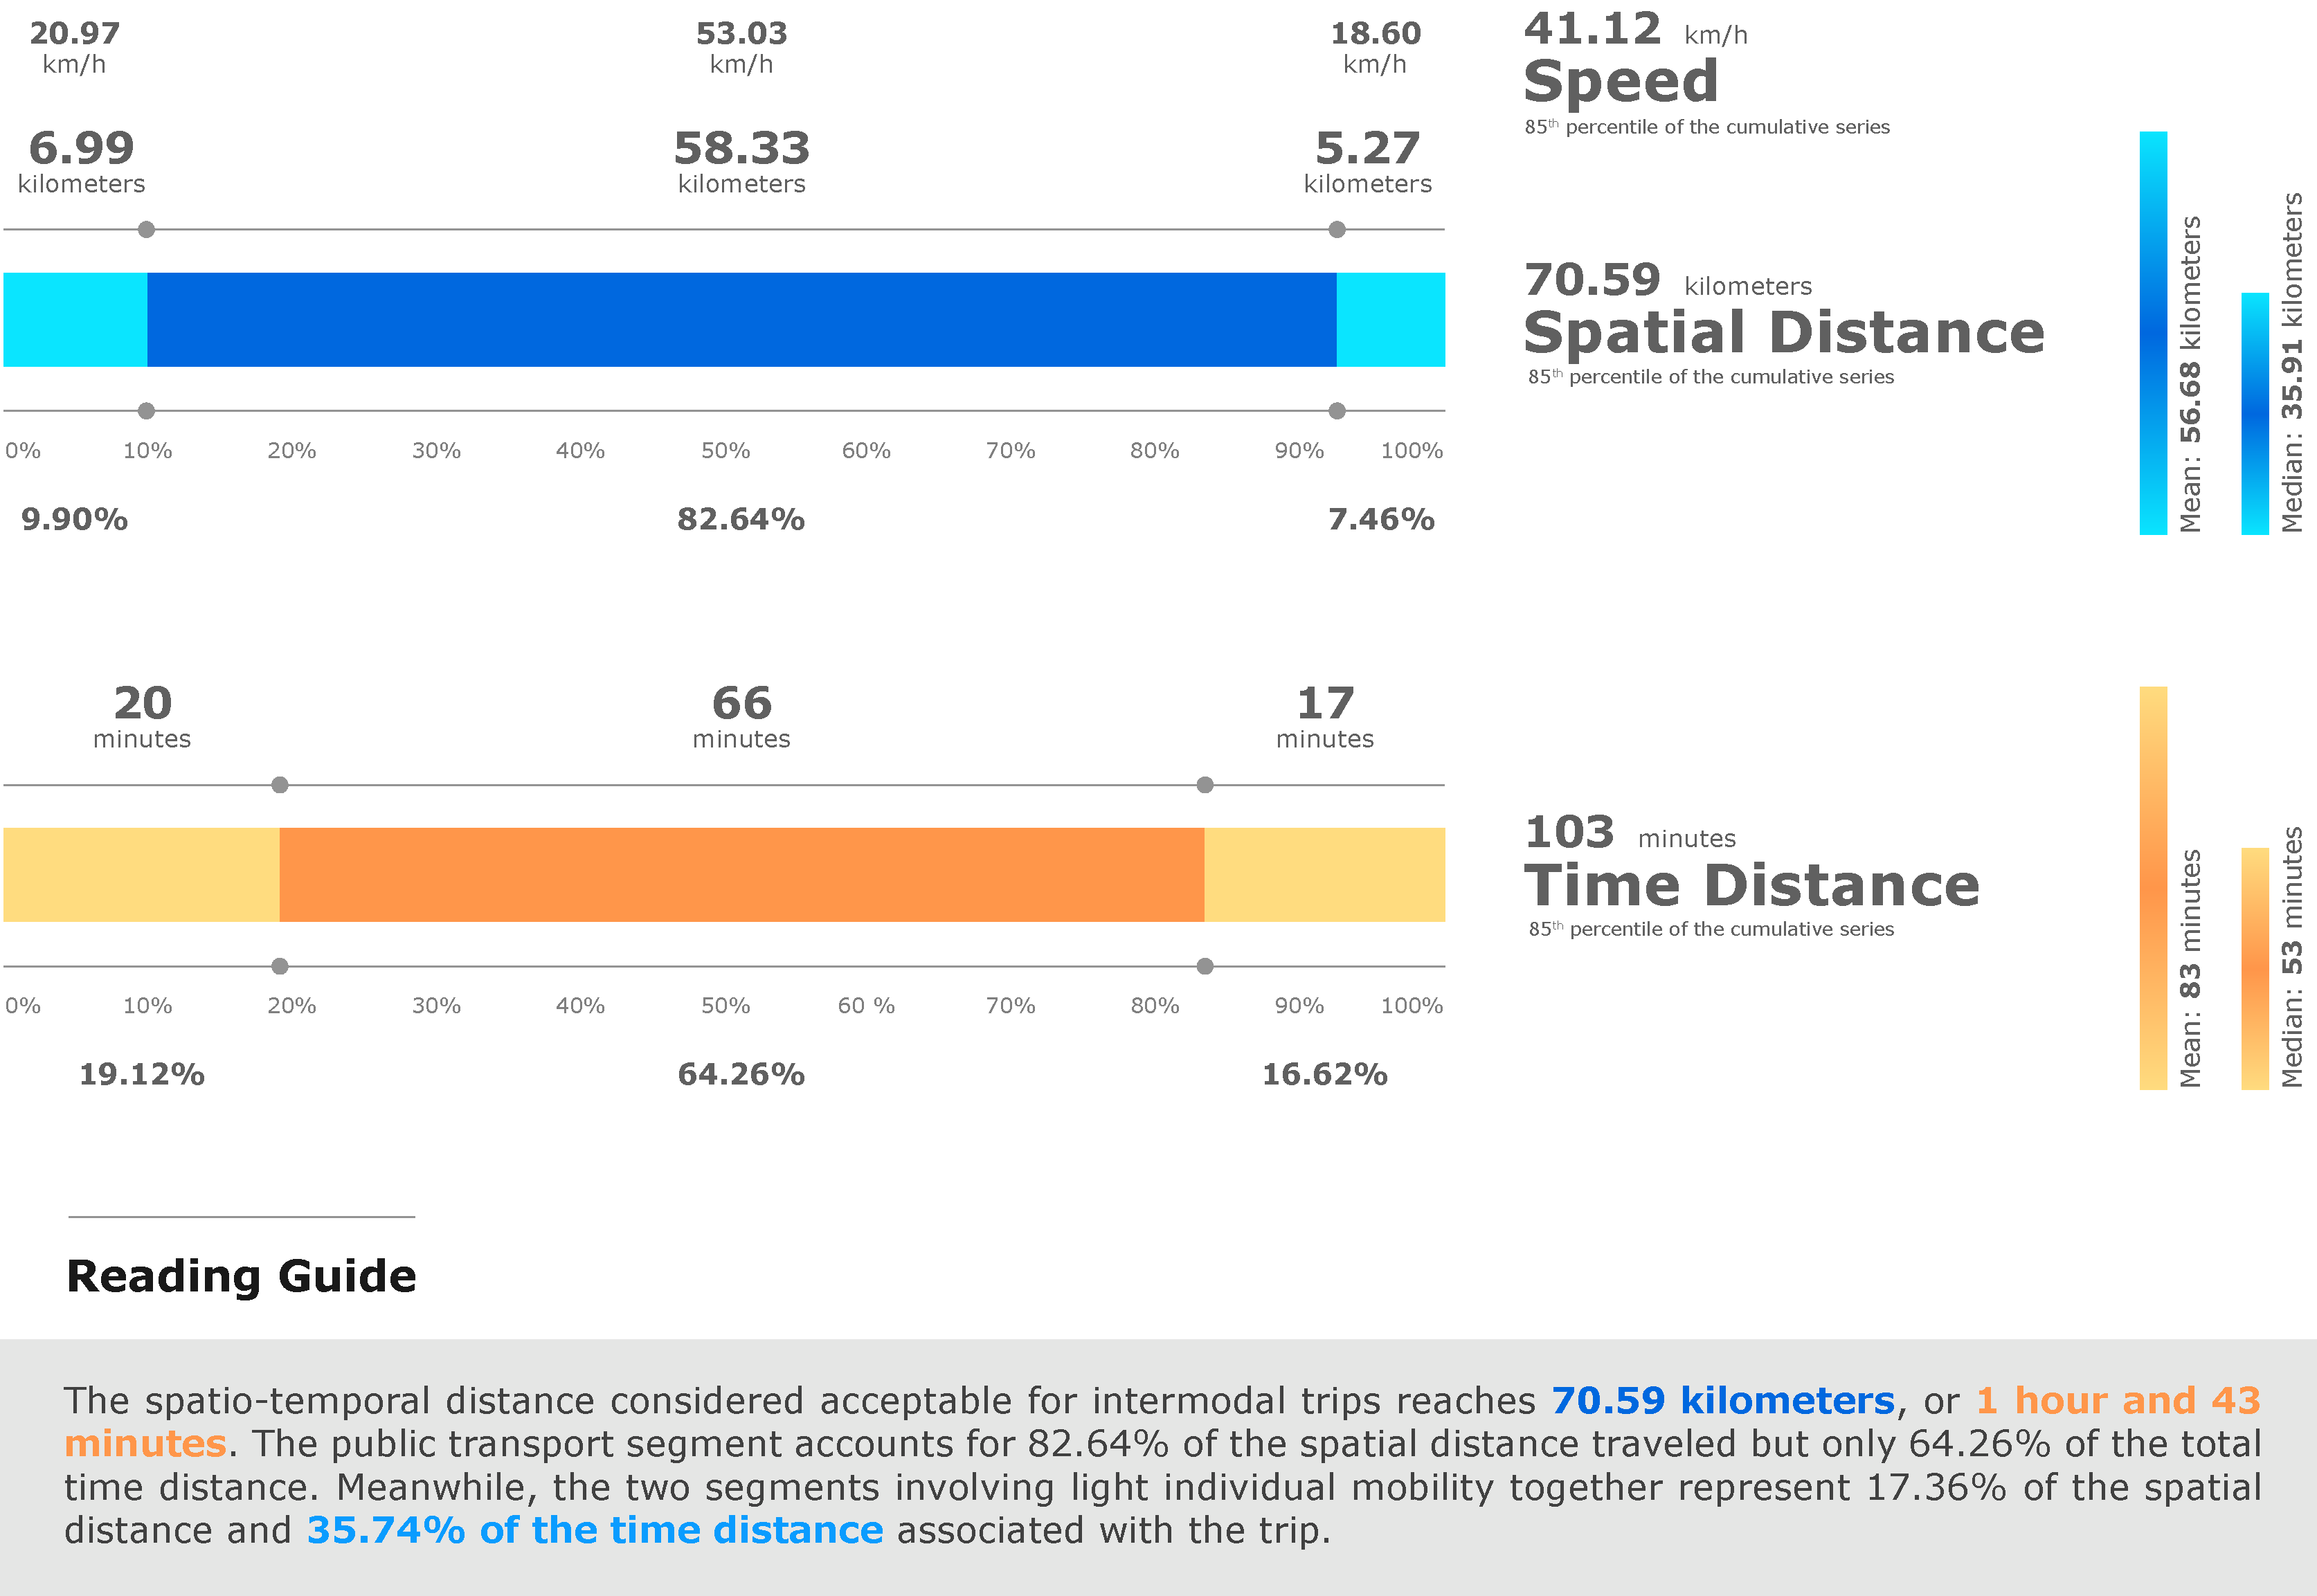
\includegraphics[width=1\columnwidth]{src/Figures/Chap-5/EN_Distances_Globales.pdf}}
    \vspace{5pt}
    \begin{flushleft}\scriptsize{
    \textcolor{blue}{Note:} the calculation of distance-time does not take into account the precautionary time when arriving at the origin station.
    }\end{flushleft}
    \begin{flushright}\scriptsize{
    Author: \textcolor{blue}{Dylan Moinse (2024)}
    }\end{flushright}
\end{figure}

% Portée de la mobilité individuelle légère et des TC
While the spatial distance of intermodal trips made using light individual mobility generally reaches 70.59 kilometers for the 85\textsuperscript{th} percentile of the cumulative series, the three segments that make up this modal chain do not contribute equally to the total distance traveled (see \hyperref[fig-chap5:distances-globales]{Figure~\ref{fig-chap5:distances-globales}}, page~\pageref{fig-chap5:distances-globales}). As expected, the public transport journey represents an average of 82.64\% of the total spatial distance traveled. Of the remaining 17.36\%, traveled by bike or micromobility, the access trip accounts for 9.90\% of the total distance, while the egress trip accounts for 7.46\%. In terms of distance-time, the average share of time spent on public transport decreases to 64.26\% of the average travel time. Of the 35.74\% of distance-time allocated to light individual mobility, 19.12\% of the time is spent on the access phase and 16.62\% on the egress phase. These data shed light on the interconnectivity ratios of light individual mobility associated with public transport—whose formula is based on dividing the distance of each segment by the total trip distance—of 0.17 in terms of spatial distance and 0.36 for the time dimension. Finally, in terms of travel speed, it averages 40.97 kilometers per hour, a lower speed than the average of 51.30 kilometers per hour observed for car drivers in France\footnote{~
    However, it is important to nuance this comparison, as the average speed by car does not account for the time required to access the vehicle or the parking time at the destination. We could therefore assume that the actual difference between the two speeds is much less significant than it initially appears.
} \textcolor{blue}{\autocite{onisr_observatoire_2022}}\index{ONISR@\textsl{ONISR}|pagebf}.%%Translated%%

% Comparaison enquêtes publiques
The total distance traveled, for home-to-work and home-to-study commutes, combining the use of light individual mobility and the public transport network, thus averages 56.68 kilometers or 1 hour and 22 minutes. This distance is significantly higher than the average spatial distance traveled by residents of the Hauts-de-France region in 2016, which was 22.9 kilometers or 28 minutes to reach their workplace \textcolor{blue}{\autocite{insee_premiere_2016}}\index{Insee@\textsl{Insee}|pagebf}. In reality, the statistical results from the trips analyzed in the online survey are close to the distances observed by \textcolor{blue}{\textcite{insee_premiere_2016}}\index{Insee@\textsl{Insee}|pagebf} concerning professional mobility from the region to the Île-de-France region, averaging 57.7 kilometers for 1 hour and 5 minutes. Focusing our attention on public transport flows, the distances measured in our study—58 minutes in public transport—roughly align with the public survey conducted by \textcolor{blue}{\textcite{ministere_de_la_transition_ecologique_et_de_la_cohesion_des_territoires_mobilite_2023}}\index{Ministère de la Transition Écologique et de la Cohésion des Territoires@\textsl{Ministère de la Transition Écologique et de la Cohésion des Territoires}|pagebf}, which indicates that a \Commas{local or long-distance} trip in France averaged 41 minutes in 2019.%%Translated%%

% Comparaison littérature scientifique
In this doctoral research, we explored the overall scope of intermodal trips, revealing a spatial distance higher than that documented in the existing scientific literature. Our secondary analysis of a survey conducted by \textsl{SNCF Réseau} determined that the average distance traveled by users of the \acrshort{PeS} in combination with the \acrshort{TER} is 40.50 kilometers, in the Provence-Alpes-Côte d'Azur region. While \textcolor{blue}{\textcite[8]{edel_potential_2021}}\index{Edel, Fabian|pagebf}\index{Wassmer, Simon|pagebf}\index{Kern, Mira|pagebf} observe that 44\% of commuting trips by \acrshort{PeS} combined with public transport exceed 20 kilometers, our statistical analysis contrasts with the distances presented in some research works. For comparison, \textcolor{blue}{\textcite[7]{rabaud_micromobilites_2019}}\index{Rabaud, Mathieu|pagebf}\index{Richer, Cyprien|pagebf} report an average distance for intermodal trips incorporating respectively bicycles, \acrshort{PBS}, and \acrshort{PeS} of 27.50; 32.30; and 22.60 kilometers in France. In combination with \acrshort{TER} or \acrshort{RER}, \textcolor{blue}{\textcite[16]{gioria_etude_2016}}\index{Gioria, Christian|pagebf} measures an average spatial distance of 39.50 kilometers for cyclists in France, with significant variations in favor of smaller urban areas. Moreover, our observations do not align with the total distances for the combination of bicycles and rail, which are 53 kilometers and 41 kilometers in the Netherlands \textcolor{blue}{\autocites[14]{shelat_analysing_2018}[225]{keijer_how_2000}}\index{Shelat, Sanmay|pagebf}\index{Huisman, Raymond|pagebf}\index{Oort, Niels van|pagebf}\index{Keijer, Majanka|pagebf}\index{Rietveld, Piet|pagebf}, or 35 kilometers in Belgium and England \textcolor{blue}{\autocite[20 ; 28]{bitibi_bike_2017}}\index{BiTiBi@\textsl{BiTiBi}|pagebf}. However, the values we obtained may resonate with the work of \textcolor{blue}{\textcite[116]{nigro_land_2019}}\index{Nigro, Antonio|pagebf}\index{Bertolini, Luca|pagebf}\index{Moccia, Francesco Domenico|pagebf}, who deduced a total distance-time for a commuting trip by train in Italy of 54 minutes. Additionally, the place of light individual mobility within intermodal trips is relatively similar to the results of their research, in which they estimated a respective duration for access and egress of 12 minutes, using the interconnectivity ratio developed by \textcolor{blue}{\textcite[274]{krygsman_multimodal_2004}}\index{Krygsman, Stephan|pagebf}\index{Dijst, Martin|pagebf}\index{Arentze, Theo|pagebf}\footnote{~
    According to \textcolor{blue}{\textcite[274]{krygsman_multimodal_2004}}\index{Krygsman, Stephan|pagebf}\index{Dijst, Martin|pagebf}\index{Arentze, Theo|pagebf}, who measured the access and egress time typically spent during intermodal trips, including those involving bicycles, the interconnectivity ratio has an average value between 0.20 and 0.50. Based on this data, \textcolor{blue}{\textcite[116]{nigro_land_2019}}\index{Nigro, Antonio|pagebf}\index{Bertolini, Luca|pagebf}\index{Moccia, Francesco Domenico|pagebf} used a threshold of 0.45 for the two segments done by bicycle.
}; as well as the study report of the European research project \textcolor{blue}{\textcite[20 ; 28]{bitibi_bike_2017}}\index{BiTiBi@\textsl{BiTiBi}|pagebf}, which reports a proportion of 11.43\%, or 4 kilometers. Furthermore, the distance of 8.93 kilometers or 24 minutes by metro, tram, and bus is corroborated by the average travel time of 12.50 kilometers or 29 minutes observed in Seoul and Daejeon, South Korea, as reported by \textcolor{blue}{\textcite[46]{lee_strategies_2010}}\index{Lee, Jaeyeong|pagebf}\index{Shin, Hee-Cheol|pagebf}. The notable gap between the limited corpus of scientific literature and our statistical results can then be attributed to an overrepresentation of trips by \acrshort{HST} in our survey, notably between Lille and Paris.%%Translated%%

% 5.1.1.4.
\needspace{1\baselineskip} % Reserve space
\subsubsection*{Determination of the Size of the \Commas{Secondary Area} of Transit-Oriented Development Areas
    \label{chap5:taille-aire-secondaire}
    }

% Portée distance euclidienne
The analysis of trips combining the use of bicycles or micromobility with public transport indicates that the \Commas{first and last kilometers} typically cover individual distances ranging from three to four kilometers, depending on the type of vehicle used. Extending this analysis using a Euclidean map, the next step is to define the size of the \acrshort{TOD} districts, considering their extension facilitated by the use of light individual mobility. As an illustration, we mapped the areas around two stations that received a significant number of responses in our survey: Lille Flandres station, located in the Nord department, and Béthune station, in Pas-de-Calais, both served by the \acrshort{HST} and \acrshort{TER} networks (see \hyperref[fig-chap5:itineraires-lille-flandres]{Map~\ref{fig-chap5:itineraires-lille-flandres}}, page~\pageref{fig-chap5:itineraires-lille-flandres} and \hyperref[fig-chap5:itineraires-bethune]{Map~\ref{fig-chap5:itineraires-bethune}}, page~\pageref{fig-chap5:itineraires-bethune}). The maps of flows and routes show that light individual mobility complements rather than competes with walking, with minimum straight-line distances of around 800 meters. The analysis also reveals that the majority of trips occur over Euclidean distances of 1 to 2 kilometers, often originating from home. For Lille station, it is interesting to note that access trips mainly come from residential neighborhoods to the east (Fives, Saint-Maurice Pellevoisin, and Marbrerie) and to the south (Gambetta and Wazemmes) of the municipalities of Lille, Hellemmes, and Ronchin, while egress trips mainly head towards the central neighborhoods, which partly explains the observed variation in distances (see \hyperref[fig-chap5:itineraires-lille-flandres]{Map~\ref{fig-chap5:itineraires-lille-flandres}}, page~\pageref{fig-chap5:itineraires-lille-flandres}). Similarly, around Béthune station, the first kilometers originate from nearby municipalities such as Nœux-les-Mines, Barlin, or Busnes, while the last kilometers are mostly directed towards activity centers in the urban center and the Beuvry hospital area (see \hyperref[fig-chap5:itineraires-bethune]{Map~\ref{fig-chap5:itineraires-bethune}}, page~\pageref{fig-chap5:itineraires-bethune}). This result can be interpreted from two complementary angles. On the one hand, it reflects a more diffuse distribution of residential areas and a higher concentration of jobs in the station district. On the other hand, it highlights, within the same territorial context and for the same station, different mobility dynamics depending on whether it is an access or egress trip.%%Translated%%

% Figure trajets autour de Lille Flandres
\begin{carte}[h!]\vspace*{4pt}
    \caption{Map of the flows and routes followed by intermodal cyclists heading to or from Lille Flandres station.}
    \label{fig-chap5:itineraires-lille-flandres}
    \centerline{\includegraphics[width=1\columnwidth]{src/Figures/Chap-5/EN_Distances_Itineraires_Lille_Flandres.png}}
    \vspace{5pt}
    \begin{flushright}\scriptsize{
    Author: \textcolor{blue}{Dylan Moinse (2024)}
    }\end{flushright}
\end{carte}

% Figure trajets autour de Béthune
\begin{carte}[h!]\vspace*{4pt}
    \caption{Map of the flows and routes followed by intermodal cyclists heading to or from Béthune station.}
    \label{fig-chap5:itineraires-bethune}
    \centerline{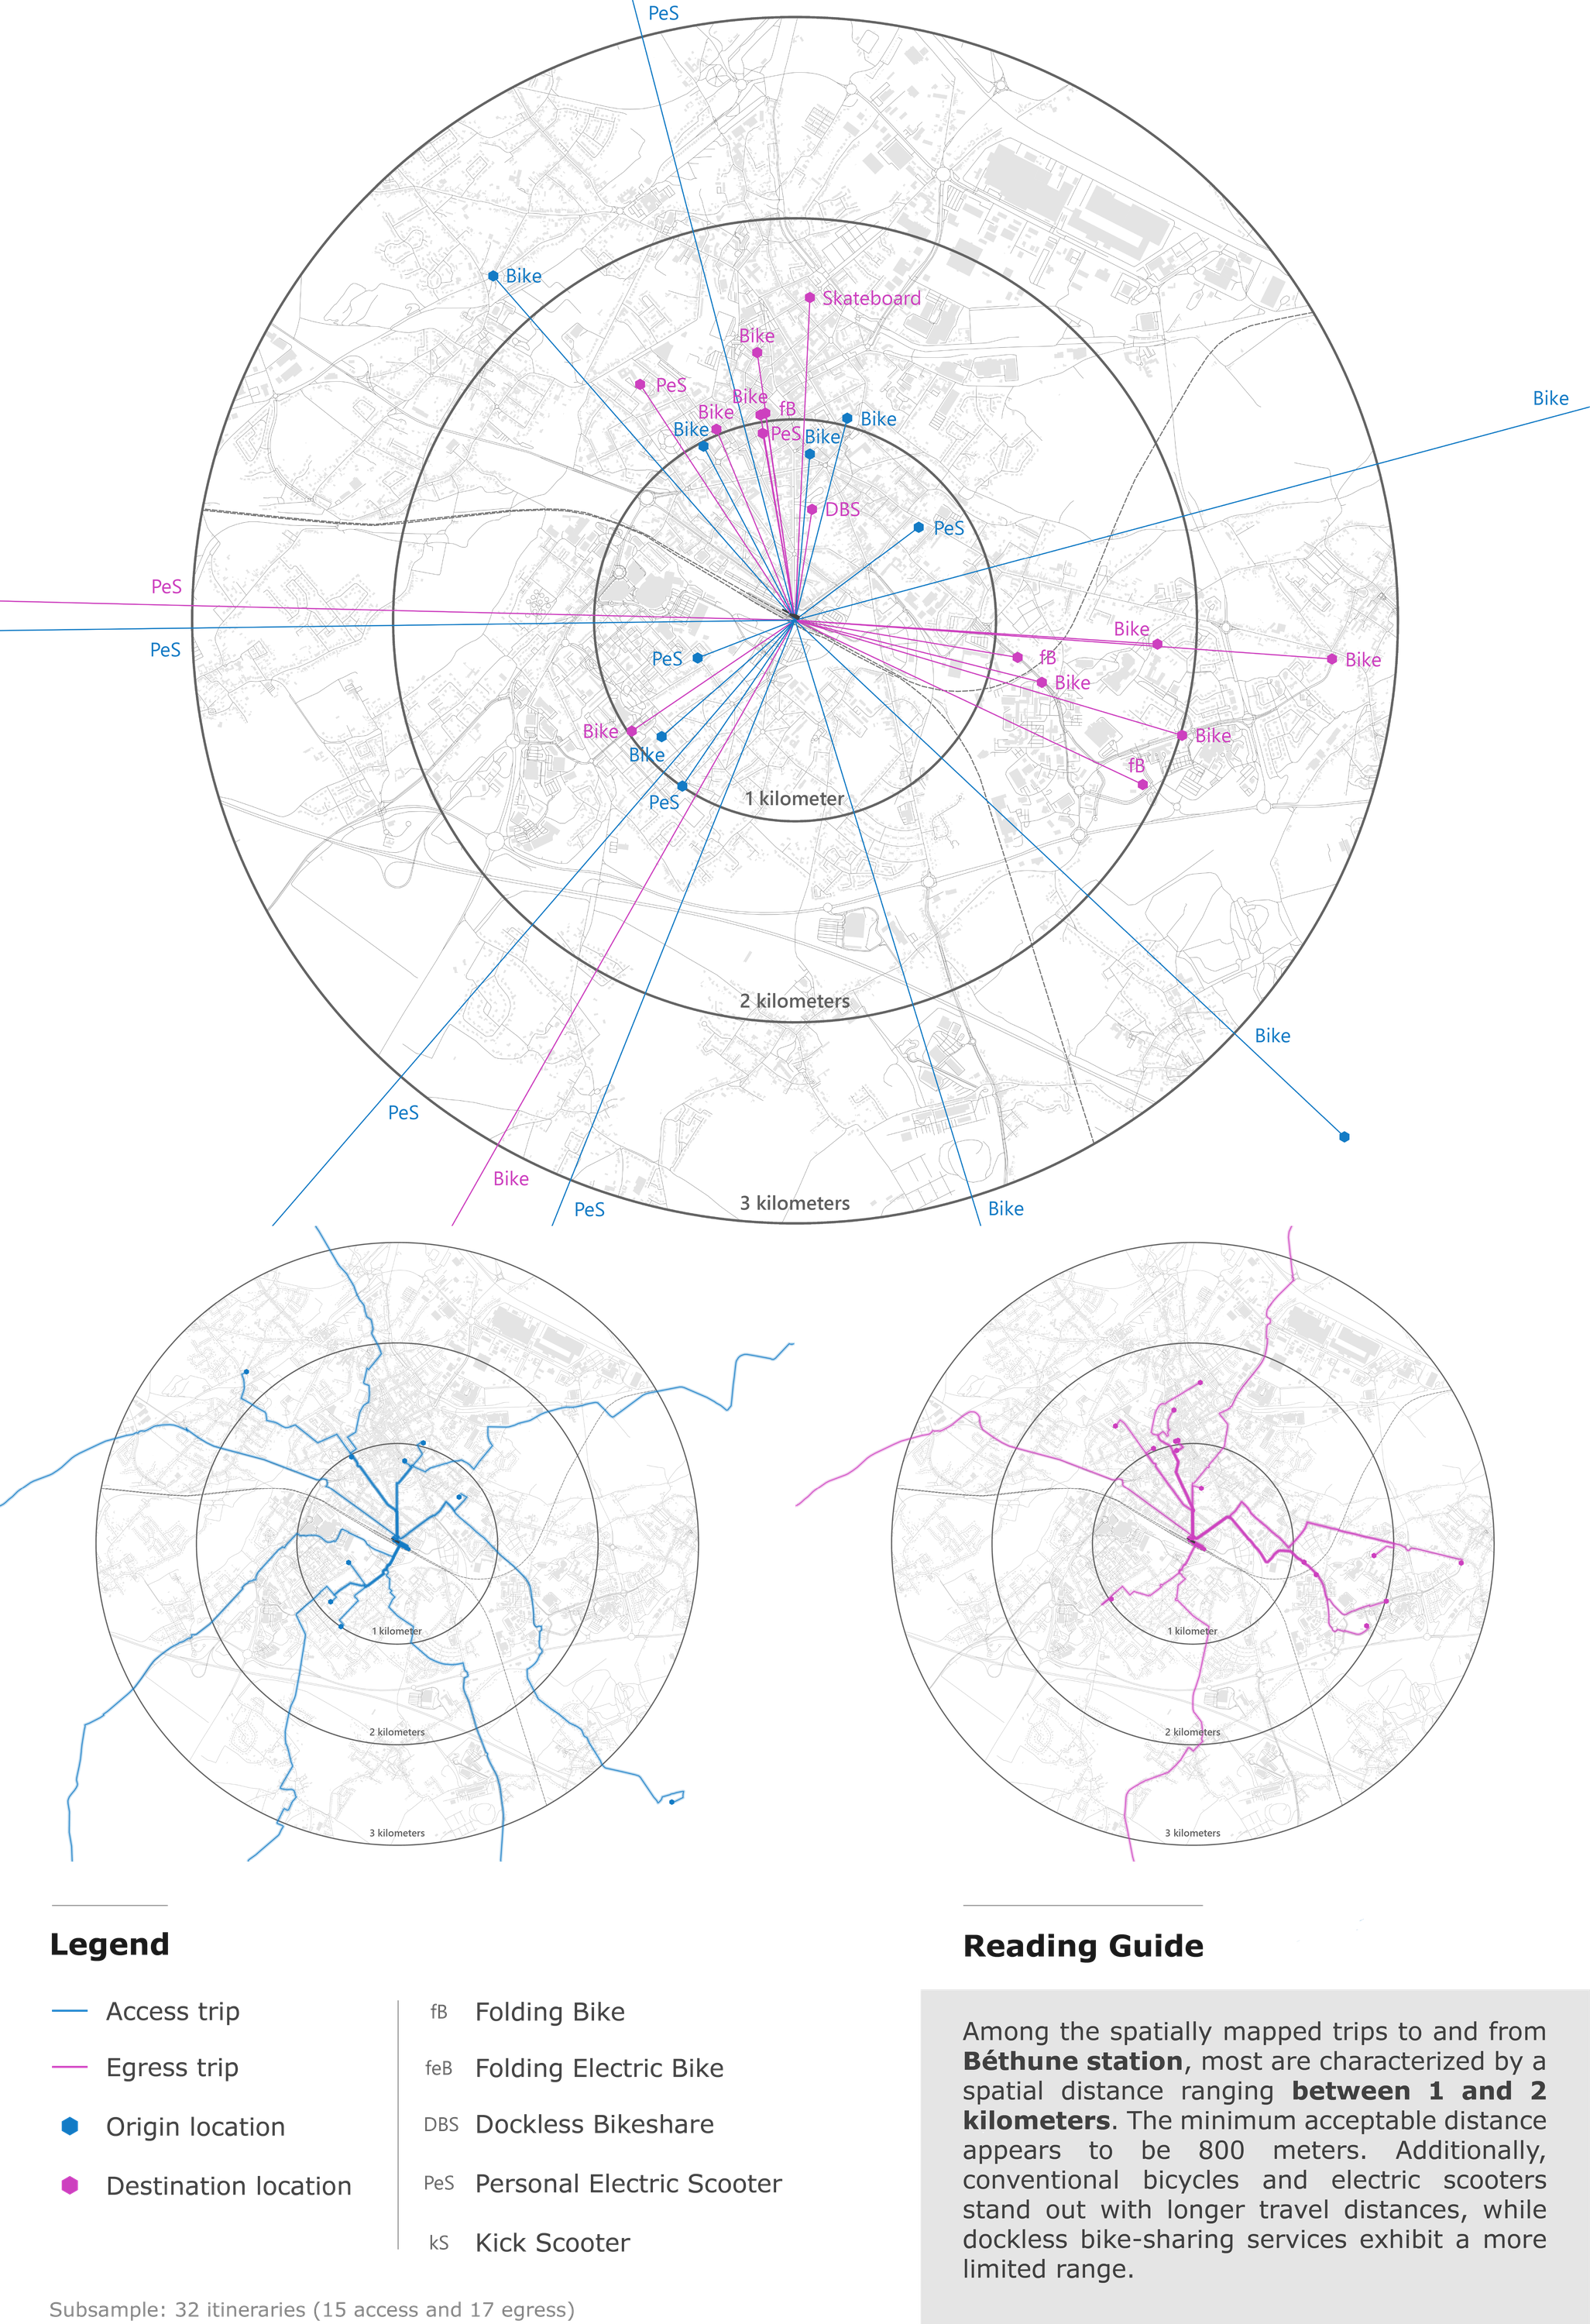
\includegraphics[width=1\columnwidth]{src/Figures/Chap-5/EN_Distances_Itineraires_Bethune.png}}
    \vspace{5pt}
    \begin{flushright}\scriptsize{
    Author: \textcolor{blue}{Dylan Moinse (2024)}
    }\end{flushright}
\end{carte}

    % Equivalent surface area
Starting from the observation that the radius of a walkable station area is typically one kilometer, while that accessible by cycling modes extends from three to four kilometers, this thesis highlights that the spatial and temporal distances traveled by bike or micromobility are three to four times greater than those covered on foot. However, it is when considering the surface area of the influence zones that the contrast becomes particularly striking. Indeed, by calculating the area of these zones—the formula for the area of a circle involves multiplying the square of the radius \(r^2\) by \(\pi\)—the cycling influence area is found to be significantly larger. For a station arean accessible by light individual mobility with a radius of 3.8 kilometers, the area reaches 45.4 square kilometers (with a circumference of 23.9 kilometers), compared to an area of 5.3 square kilometers (with a circumference of 8.2 kilometers) for a walkable range of 1.3 kilometers. This means that light individual mobility allows for a considerable increase in local accessibility around public transport hubs, multiplying the size of the walkable area by 8.54 times.%%Translated%%

    % Breaking the bubble
It should be added that the size of the pedestrian perimeter, established using the responses to the survey, exceeds that typically observed in academic works, urban planning documents, and operational studies, where the spatial limit for walking trips, both for access and egress, is usually set between 500 and 800 meters \textcolor{blue}{\autocite[133]{pojani_transit-oriented_2015}}\index{Pojani, Dorina|pagebf}\index{Stead, Dominic|pagebf}. The delimitation of pedestrian accessibility up to 1.3 kilometers illustrates the extension of the idea of \Commas{bursting the bubble}, a term borrowed from \textcolor{blue}{Brian} \textcolor{blue}{\textcite[34]{canepa_bursting_2007}}\index{Canepa, Brian|pagebf}, Project Manager at the consulting firm \textsl{W-Trans}. In his scientific article entitled \textsl{Bursting the Bubble. Determining the Transit-Oriented Development’s Walkable Limits}, he invites researchers and practitioners to question the orthodoxy of a 500-meter walking limit around \acrshort{TOD} neighborhoods. The redefinition of this limit is supported by the literature review conducted by \textcolor{blue}{Alain} \textcolor{blue}{\textcite[5]{lhostis_perimetres_2016}}\index{L'Hostis, Alain|pagebf}, who challenges the relevance of the arbitrary 800-meter barrier, equivalent to the 0.5-mile rule, and advocates for its extension, a position also supported by \textcolor{blue}{\textcite[79]{ker_myths_2003}}\index{Ker, Ian|pagebf}\index{Ginn, Simon|pagebf} who label this limit as a myth or a dogma. Consequently, our research contributes to the deconstruction of this preconceived bubble on two distinct levels: the area of \acrshort{TOD} neighborhoods increases from 2.01 square kilometers (for a 0.8-kilometer radius) to 5.31 square kilometers (for 1.3 kilometers) regarding walking, and extends up to 45.36 square kilometers (for 3.8 kilometers) for cycling and micromobility. Thus, the determination of a station neighborhood based on declared mobility practices leads us to consider an area up to 2.64 times larger for walking and 22.57 times larger thanks to light individual mobility.%%Translated%%

    % Figure influence areas
    \begin{carte}[h!]\vspace*{4pt}
        \caption{Area occupied by the extension of pedestrian and cycling station neighborhoods, at the scale of the Hauts-de-France region.}
        \label{fig-chap5:aires-influence}
        \centerline{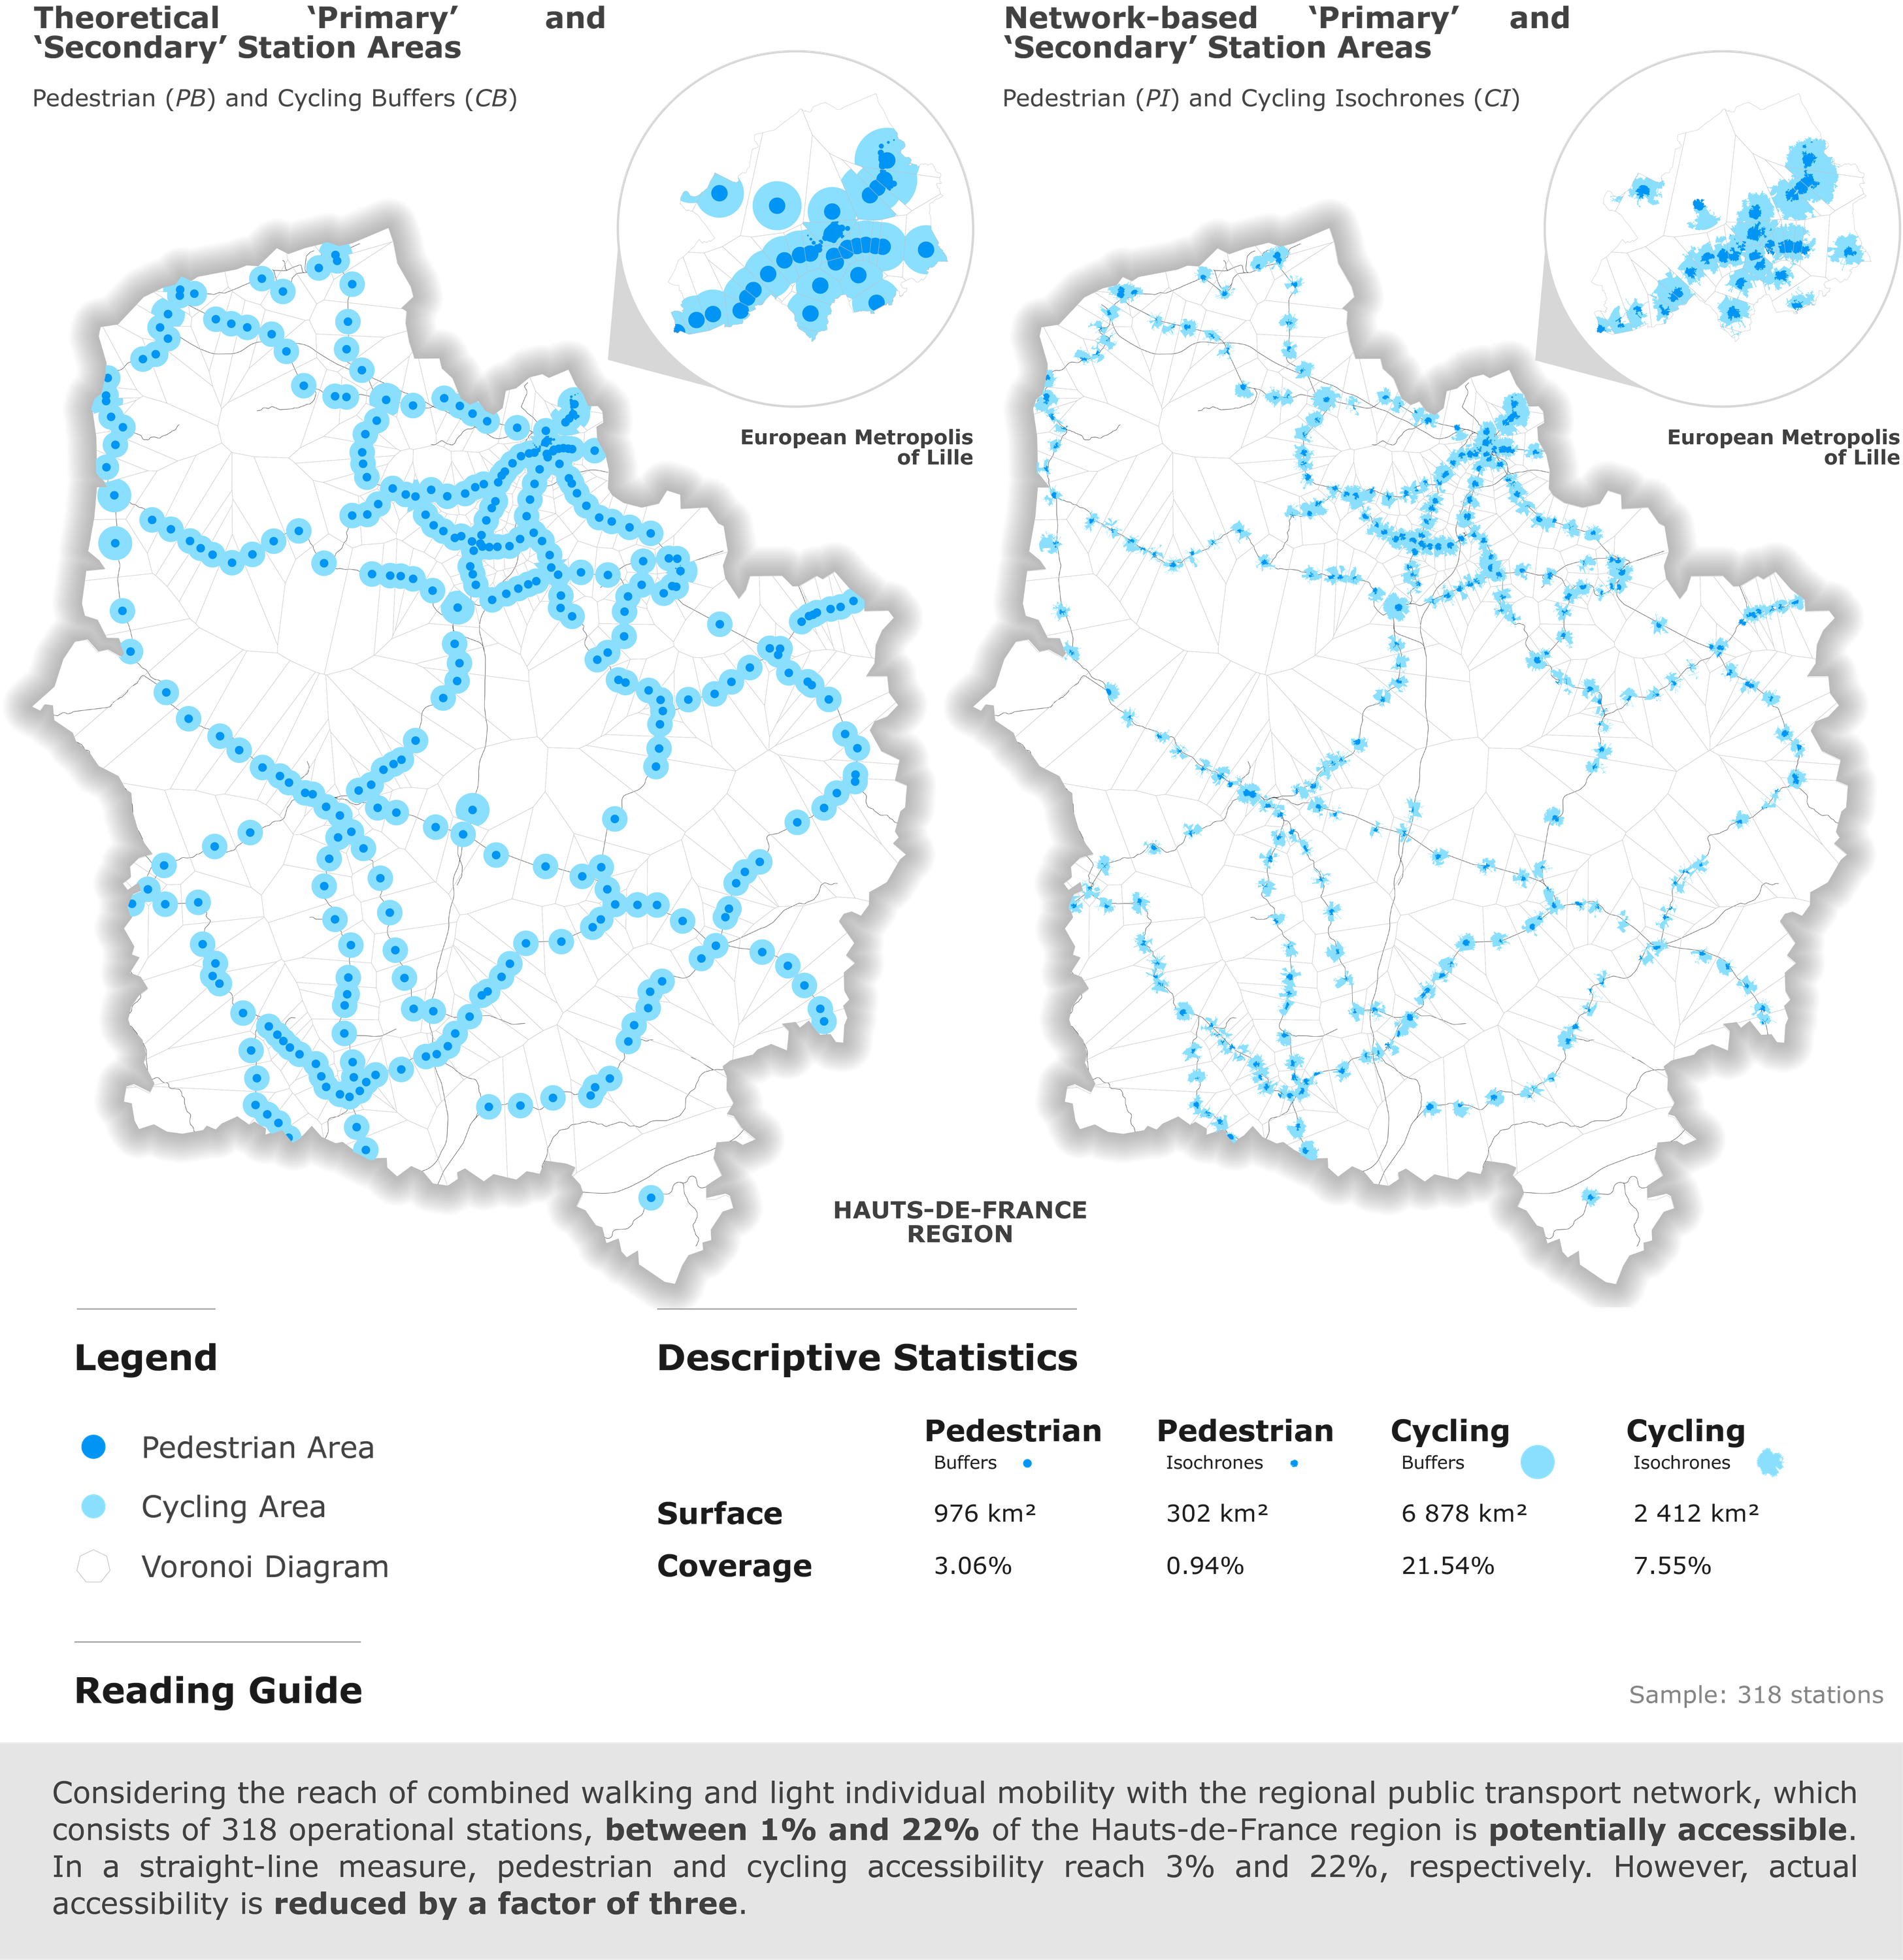
\includegraphics[width=1\columnwidth]{src/Figures/Chap-5/EN_Distances_Aires_influence.png}}
        \vspace{5pt}
        \begin{flushright}\scriptsize{
        Author: \textcolor{blue}{Dylan Moinse (2024)}
        }\end{flushright}
    \end{carte}

    % Influence areas
By extrapolating this estimated distance threshold across the 318 stations currently in operation in the Hauts-de-France region, this research suggests that combined walking provides access to 3.06\% of the territory’s surface area by straight-line distance, and to 0.94\% of the territory when accounting for the existing pedestrian infrastructure (see \hyperref[fig-chap5:impedance-distances]{Map~\ref{fig-chap5:aires-influence}}, page~\pageref{fig-chap5:aires-influence}). The introduction of light individual mobility raises territorial accessibility to 21.54\% of the region by straight-line distance, and to 7.55\% when considering the road network accessible by bike (see \hyperref[fig-chap5:impedance-distances]{Map~\ref{fig-chap5:aires-influence}}, page~\pageref{fig-chap5:aires-influence}). However, the disparities between buffer zones and isodistances also shed light on the compression of accessibility potential due to the presence of physical barriers and the urban fabric, which tend to reduce actual pedestrian accessibility by a factor of 3.26 and cycling accessibility by a factor of 2.85. Beyond this discussion on accessible areas, we will explore which aspects most influence the variability of the established distances.%%Translated%%

    % 5.1.2.
    \needspace{1\baselineskip} % Reserve space
\subsection{Influence of Built Environment and Individual Characteristics on Spatial Distances Traveled
    \label{chap5:regression-distances}
    }

    % Objective
After establishing the spatial and temporal distance thresholds considered acceptable by users, our research shifted towards analyzing the impact of various factors related to the characteristics of the territories traversed, the behaviors and mobility habits of intermodal travelers, as well as their socio-demographic profile on the variability of the estimated distances. To do this, we employed the Ordinary Least Squares (OLS) regression method, a statistical technique recognized for its effectiveness in estimating the relationships between a dependent variable—in this case, distance—and several independent variables. This method has the advantage of minimizing the sum of the squared residuals, that is, the differences between the observed values and those predicted by the multiple regression model, which is found to be the best fit for the collected data.%%Translated%%

    % 5.1.2.1.
    \needspace{1\baselineskip} % Reserve space
\subsubsection*{Application of a Linear Regression Model Coupled with a Constant Elasticity Model
    \label{chap5:modeles-OLS-log-log}
    }

    % OLS Methodology
The application of this regression allows us to determine the coefficients of determination, denoted R\textsuperscript{2} and adjusted R\textsuperscript{2}. The R\textsuperscript{2} indicates the proportion of the total variance of the dependent variable that is explained by the independent variables in the model. However, given the presence of a substantial number of predictors in our model, which may artificially influence the R\textsuperscript{2}, we place particular importance on the adjusted R\textsuperscript{2}. This latter measure has the advantage of reducing the R\textsuperscript{2} value when the addition of additional variables to the model does not significantly contribute to improving the model's ability to explain the observed variance, thereby penalizing the inclusion of unnecessary variables.%%Translated%%

    % Log-log Modeling
In addition to the ordinary least squares regression, a log-log modeling approach, also referred to as a double logarithmic model or constant elasticity model, has been implemented. This method aims to estimate elasticities, that is, the proportional sensitivity of the dependent variable, in this case, distance, to changes in the independent variables. This type of model provides a distinct analytical approach that enhances the understanding of interactions between the variables by measuring the effects proportionally through the coefficient of determination \(\beta\). This particular perspective thus allows for an assessment of the proportional effects of the independent variables on the dependent variable.%%Translated%%

    % Factors surveyed
As part of this statistical model, the two regressions were based on a range of independent variables, extracted both from the questionnaire distributed to users and from the subsequent statistical and spatial analysis. These variables are listed below:
\begin{customitemize}
    \item The type of transfer mode involved;
    \item The boarding methods or the type of parking adopted for the vehicle;
    \item The public transport system;
    \item The effect of modal substitution;
    \item The distance-time of the access or egress trip;
    \item The demographic density around the origin or destination points;
    \item The terrain elevation;
    \item The perceived comfort level of the access and egress routes;
    \item The trip purpose;
    \item The usage frequency;
    \item The intermodal experience of users;
    \item The mobility habits of users;
    \item The household composition;
    \item Bicycle ownership within the household;
    \item The motorization rate of the household;
    \item The gender of users;
    \item The age of users;
    \item The professional situation of users;
    \item The professional activity sector of users;
    \item The educational level of users;
    \item The annual disposable income of users.
\end{customitemize}%%Translated%%

    % 5.1.2.2. 
    \needspace{1\baselineskip} % Reserve space
\subsubsection*{Determinants of Spatial Distances Traveled
    \label{chap5:facteurs-modeles-OLS-log-log}
    }

    % General Results
The overall coefficient of determination for the model is 0.90, while the adjusted R\textsuperscript{2} reaches 0.79. This result indicates that 90.20\% of the variability of the dependent variable is explained by the independent variables included in the model. The presence of an adjusted R\textsuperscript{2} significantly lower than the raw R\textsuperscript{2} suggests that some variables included in the analysis do not contribute significantly to explaining the observed variance in the distance variable. To correct for potential overfitting, it is proposed to remove certain variables from the ordinary least squares model. These exclusions concern the boarding methods or the type of parking adopted for the vehicle, modal substitution effects, except those involving car use, mobility habits other than walking, as well as variables related to bicycle and car ownership, age, professional situation, educational level, and the disposable income of travelers.%%Translated%%

    % Tableau corrélation facteurs
% Correlation factors table
%%Translated%%
    \begin{table}[h!]
    \centering
    \renewcommand{\arraystretch}{1.5}
    \resizebox{\columnwidth}{!}{
    \begin{tabular}{p{0.46\columnwidth}p{0.14\columnwidth}p{0.16\columnwidth}p{0.11\columnwidth}p{0.13\columnwidth}}
        %\hline
    \rule{0pt}{15pt} \multirow{1.5}{*}{\small{\textbf{\textcolor{blue}{Independent Variables}}}} & \small{\textbf{\textcolor{blue}{Elasticity \(\beta\)}}} & \small{\textbf{\textcolor{blue}{R\textsuperscript{2} Coefficient}}} & \small{\textbf{\textcolor{blue}{P-value}}} & \multirow{1.5}{*}{\textbf{\textcolor{blue}{$\sigma$}}}\\
        \hline
\small{Type of light individual mobility} & \small{\textbf{1.54\%}} & \small{1,815.23} & \small{0.13} & \small{1,413.59}\\
\small{Travel time**} & \small{\textbf{1.21\%}} & \small{286.51} & \small{0.00} & \small{8.87}\\
\small{Usage frequency**} & \small{\textbf{0.73\%}} & \small{652.86} & \small{0.01} & \small{479.09}\\
\small{Professions (\acrshort{PCS})*} & \small{\multirow{1.5}{*}{\textbf{0.64\%}}} & \small{\multirow{1.5}{*}{196.93}} & \small{\multirow{1.5}{*}{0.05}} & \small{\multirow{1.5}{*}{994.67}}\\
\small{Household size*} & \small{\textbf{0.54\%}} & \small{2,166.65} & \small{0.05} & \small{1,110.77}\\
\small{Public transport system**} & \small{\textbf{0.46\%}} & \small{1,262.87} & \small{0.00} & \small{393.99}\\
\small{Car substitution} & \small{\textbf{0.40\%}} & \small{616.49} & \small{0.23} & \small{516.99}\\
\small{Travel purpose} & \small{\textbf{0.28\%}} & \small{491.88} & \small{0.25} & \small{430.49}\\
\small{Gender} & \small{\textbf{0.17\%}} & \small{-279.85} & \small{0.28} & \small{609.83}\\
\small{Population density} & \small{\textbf{-0.01\%}} & \small{-0.02} & \small{0.16} & \small{0.01}\\
\small{Comfort perception} & \small{\textbf{-0.13\%}} & \small{-40.41} & \small{0.15} & \small{82.90}\\
\small{Terrain slope**} & \small{\textbf{-0.13\%}} & \small{-5.81} & \small{0.04} & \small{2.77}\\
\small{Intermodal experience} & \small{\textbf{-0.23\%}} & \small{-357.81} & \small{0.45} & \small{752.37}\\
\small{Frequent walking practice**} & \small{\textbf{-0.32\%}} & \small{-284.01} & \small{0.01} & \small{109.53}\\
        \hline
        \end{tabular}}
    \caption{Descriptive statistics of the constant elasticity model measuring the proportional effects of independent variables on spatial distance in light individual mobility.}
    \label{table-chap5:facteurs-distance-spatiale}
        \vspace{5pt}
        \begin{flushleft}\scriptsize{
        \textcolor{blue}{Note:} **$p$\textless0.05, *$p$\textless0.10, $\sigma$ corresponds to the standard deviation.
        \\
        \textcolor{blue}{Reading Guide:} All else being equal, when an independent variable increases by 1\%, the distance value increases by $X$\%.
        }\end{flushleft}
        \begin{flushright}\scriptsize
        Author: \textcolor{blue}{Dylan Moinse (2023)}
        \end{flushright}
        \end{table}%%Rédigé%%

    % Results positive and negative influence
The elasticity analysis within the regression model reveals that the variables exerting a predominant influence on the spatial distance traveled by users of light individual mobility and public transport mainly include the form of modal combination, trip duration, usage frequency, \acrfull{PCS}, household composition, car substitution, walking regularity, and trip purpose (see \hyperref[table-chap5:facteurs-distance-spatiale]{Table~\ref{table-chap5:facteurs-distance-spatiale}}, page~\pageref{table-chap5:facteurs-distance-spatiale}). Keeping other variables constant, it appears that if the distance-time increases by 1\%, the corresponding spatial distance increases by 1.21\%. Similarly, a 1\% increase in usage frequency results in a 0.73\% increase in the distance traveled. Regarding the modal combination, a 1\% increase in the probability of bike use leads to a 1.54\% increase in the distance traveled, while the use of the \acrshort{HST} increases the distance by 0.46\%. Furthermore, statistical analysis shows that spatial distance experiences a positive variation when the user tends to be a senior executive (0.64\%) or a man (0.17\%), when the household expands (0.54\%), or when the trip is utilitarian (0.28\%). Conversely, all else being equal, the distance traveled tends to decrease by 0.32\% when the user regularly walks, and by 0.23\% when the user has recently adopted more intermodal practices.%%Translated%%

    % Results no notable influence
These observations highlight the factors influencing the spatial distance of trips, illustrating the impact of modal choices, travel habits, as well as individual characteristics on the extent of journeys. The regression presented in \hyperref[table-chap5:facteurs-distance-spatiale]{Table~\ref{table-chap5:facteurs-distance-spatiale}} (page~\pageref{table-chap5:facteurs-distance-spatiale}) also demonstrates that certain factors have a negligible impact on this relationship, such as population density (0.01\%), or a minor one, such as the subjective evaluation of route quality (-0.13\%) or terrain elevation (-0.13\%). These statistical results align with the research conducted by \textcolor{blue}{\textcite[181]{gan_associations_2021}}\index{Gan, Zuoxian|pagebf}\index{Yang, Min|pagebf}\index{Zeng, Qingcheng|pagebf}\index{Timmermans, Harry~J.~P.|pagebf} in Nanjing, which found no significant link between demographic density and the distance traveled by bike around metro stations. While the negative impact of slopes on the relationship between users and distance is not surprising, the negative effect of comfort perception might seem counterintuitive. However, it is plausible that the quality rating of routes reported by travelers decreases precisely because longer distances often involve more complex routes, generally located outside urban centers. This hypothesis was also discussed by \textcolor{blue}{\textcite[185]{gan_associations_2021}}\index{Gan, Zuoxian|pagebf}\index{Yang, Min|pagebf}\index{Zeng, Qingcheng|pagebf}\index{Timmermans, Harry~J.~P.|pagebf}, who also found that the experience of comfort while cycling is negatively correlated with the distances traveled, suggesting that the urban environment traversed by longer trips tends to be rated more negatively.%%Translated%%

% Results access VS egress
By distinguishing, within the regression model, trips made from home versus those directed towards the activity location, nuances in the effects of certain factors emerge. While the influence of travel time on spatial distance remains constant (1.25\% for access and 1.18\% for egress), the impact of modal substitution away from car use varies significantly. Thus, in the access phase, elasticity reaches 0.60\% for former drivers and 0.50\% for former passengers, while in the egress phase, these values are reversed to -0.28\% and -0.31\%, respectively. This noticeable difference can partly be explained by the fact that access trips, initially made by car, are generally longer than those made towards the activity location. A second notable element concerns the asymmetry of the impact of household size, which manifests differently across the segments of intermodal travel: households consisting of one or two parents with one or more children tend to be less sensitive to an increase in access distances (elasticity of demand of 0.62\% and 0.33\%), while an opposite effect is observed during egress (elasticity of -0.30\% and -0.38\%) compared to households without children. This dynamic suggests the existence of a travel chain made prior to the main public transport journey, primarily for child accompaniment. Responses to the questionnaire, especially the question \Commas{Did you make an intermediate stop during your [access or egress] trip?}, where 37 participants indicated having made an intermediate stop for accompaniment purposes, illustrate this trend. Among these 37 respondents, 17 are part of a household with one or more children (45.95\%), a proportion higher than that observed in the overall population targeted by the survey, which includes 74 households with children, representing 33.94\% of the total sample.%%Translated%%

    % Transition
This analysis of the distances traveled during the \Commas{first and last miles} of public transport systems highlights a diversity of intermodal practices influenced by various personal and contextual factors. From this perspective, we are led to address the following question in the next subsection: what are the accessibility gains at the regional scale generated by the intermodal use of light individual mobility? This shift from a local scale to a regional perspective allows us to better understand how the extension of station neighborhoods can reshape regional accessibility.%%Translated%%
    
     % ___________________________________________
    % 5.2.
    \newpage
    \needspace{1\baselineskip} % Reserve space
    \sectionheader{Regional Accessibility Gains}
\section{Intermodal Accessibility Gains made Possible by the Extension of Influence Areas around Public Transport Network Nodes
    \label{chap5:accessibilite-intermodale-extension-aire-influence}
    }

    % Introduction
The extension of influence areas around public transport network nodes generates considerable gains in terms of \gls{intermodal accessibility}, notably through the integration of light individual mobility. The rise of intermodal services and the resulting mobility practices require a holistic approach to the territorial performance of the transport system, going beyond a sectoral evaluation. Indeed, measuring only physical distance appears insufficient, as it does not account for the social dimension of accessibility, which incorporates a contextual and particular aspect \textcolor{blue}{\autocite[3]{lhostis_definir_2010}}\index{L'Hostis, Alain|pagebf}\index{Conesa, Alexis|pagebf}\index{Arnaud Banos, Thomas Thévenin|pagebf}. It is therefore imperative to review the methods for evaluating transport provision and accessibility calculations, taking into account the variety of modal combinations and their relative effectiveness \textcolor{blue}{\autocite[111]{chapelon_transports_2016}}\index{Chapelon, Laurent|pagebf}. In this regard, we examine in this section how this spatial extension can improve regional accessibility in light of the potential for modal shift expressed through the population's access to the mobility system, as well as to jobs and \acrfull{POIs}. Addressing the issue of intermodal accessibility, this analysis is structured around several subsections, successively exploring the \hyperref[chap5:couverture-population]{improvement of station access potential by the population} (page~\pageref{chap5:couverture-population}) and the \hyperref[chap5:accessibilite-emplois]{gains in accessibility to employment areas and various territorial attraction points} (page~\pageref{chap5:accessibilite-emplois}).%%Translated%%

    % 5.2.1.
    \needspace{1\baselineskip} % Reserve space
\subsection{Improvement of the Population Coverage Potential by the Public Transport System
    \label{chap5:couverture-population}
    }

    % Introduction
The integration of light individual mobility within the public transport network is a crucial element for evaluating a revisited \acrshort{TOD} model in the region in question. In this subsection, we discuss the implications of intermodal accessibility gains in terms of regional geographic and demographic coverage, as well as the potential for modal shift towards this mobility system. In this regard, we first examine the share of the population served by the expansion of station influence areas. Then, we characterize the demographic density of these areas and consider the contours of an accessibility that aims to be more inclusive.%%Translated%%

    % 5.2.1.1.
    \needspace{1\baselineskip} % Reserve space
\subsubsection*{Towards a Threefold Increase in the Modal Shift Potential towards the Regional Public Transport Network
    \label{chap5:couverture-regionale}
    }

    % Regional accessibility gains
The extension of station neighborhoods enabled by the rise of light individual mobility implies an improvement in the territorial coverage of the public transport system at the regional scale. As shown in \hyperref[table-chap5:couverture-spatiale]{Table~\ref{table-chap5:couverture-spatiale}} (page~\pageref{table-chap5:couverture-spatiale}) and \hyperref[fig-chap5:impedance-distances]{Map~\ref{fig-chap5:aires-influence}} (page~\pageref{fig-chap5:aires-influence}) presented in the \hyperref[chap5:taille-aire-secondaire]{previous section} dealing with the determination of station neighborhood size (page~\pageref{chap5:taille-aire-secondaire}), the area effectively accessible on foot is multiplied by eight due to the expansion of light individual mobility's reach. With a regional area of 31,936 square kilometers, the \Commas{primary} actual area extends over 302 square kilometers, while the \Commas{secondary} actual area covers 2,110 square kilometers, thus, the total influence area is 2,412 square kilometers. Consequently, the regional coverage of \acrshort{TOD} neighborhoods increases from 0.94\% to 7.55\%, with a potential reaching up to 18.48\% (6,878 square kilometers) of the region, when considering the effects of \gls{urban barrier} and physical barriers.%%Translated%%

    % Population accessibility
By closely examining the population coverage at the regional scale, it appears that the station neighborhoods accessible on foot, taking into account the road network, cover 19.52\% of the population of Hauts-de-France, or 1,170,135 inhabitants. Furthermore, the \Commas{secondary} area alone is able to cover more than one-third of the regional population, representing 36.18\% of the inhabitants, or 2,169,229 people. Thus, station neighborhoods accessible to both pedestrians and cyclists allow for the coverage of more than half of the regional population, equivalent to 55.70\% or 3,339,364 residents (see \hyperref[table-chap5:couverture-spatiale]{Table~\ref{table-chap5:couverture-spatiale}}, page~\pageref{table-chap5:couverture-spatiale}). From this perspective, the combined perimeter of station neighborhoods, both pedestrian and cycling, extends 8.03 times that limited to pedestrian reach and encompasses 2.85 times more residents benefiting from access to the stations.%%Translated%%

    % Tableau couverture population régionale
% Regional population coverage table
%%Translated%%
    \begin{table}[h!]
    \centering
    \renewcommand{\arraystretch}{1.5}
    \resizebox{\columnwidth}{!}{
    \begin{tabular}{p{0.33\columnwidth}p{0.12\columnwidth}p{0.12\columnwidth}p{0.15\columnwidth}p{0.13\columnwidth}p{0.15\columnwidth}}
        %\hline
    \rule{0pt}{15pt} \multirow{1.5}{*}{\small{\textbf{\textcolor{blue}{Geographical Area}}}} & \small{\textbf{\textcolor{blue}{Distances (km)}}} & \small{\textbf{\textcolor{blue}{Distances (min)}}} & \small{\textbf{\textcolor{blue}{Region Area (\%)}}} & \small{\textbf{\textcolor{blue}{Population (\%)}}} & \small{\textbf{\textcolor{blue}{Density (inhab/km\textsuperscript{2})}}}\\
        \hline
\small{Pedestrian isochrones} & \small{\textless1} & \small{\textless12} & \small{0.94} & \small{19.52} & \small{3,880.25}\\
\small{Pedestrian areas} & \small{\textless1} & \small{\textless12} & \small{3.06} & \small{25.27} & \small{1,552.20}\\
        \hdashline
\small{Cyclable isochrones} & \small{{[}1~;~4{[}} & \small{\textless12} & \small{6.61} & \small{36.18} & \small{1,028.07}\\
\small{Cyclable areas} & \small{{[}1~;~4{[}} & \small{\textless12} & \small{18.48} & \small{40.13} & \small{407.68}\\
        \hdashline
\small{Pedestrian and cyclable isochrones} & \multirow{1.5}{*}{\small{\textless4}} & \multirow{1.5}{*}{\small{\textless12}} & \multirow{1.5}{*}{\small{7.55}} & \multirow{1.5}{*}{\small{55.70}} & \multirow{1.5}{*}{\small{1,384.73}}\\
\small{Pedestrian and cyclable areas} & \small{\textless4} & \small{\textless12} & \small{21.54} & \small{65.40} & \small{570.13}\\
        \hdashline
\small{Non-accessible isochrones} & \small{\Geq 4} & \small{\Geq 12} & \small{92.45} & \small{44.30} & \small{89.96}\\
\small{Non-accessible areas} & \small{\Geq 4} & \small{\Geq 12} & \small{78.46} & \small{34.60} & \small{82.77}\\
        \hline
        \end{tabular}}
    \caption{Regional population coverage by the rail network supported by light individual mobility.}
    \label{table-chap5:couverture-spatiale}
        \vspace{5pt}
        \begin{flushleft}\scriptsize{
        \textcolor{blue}{Note:} The average population density in the Hauts-de-France region was 189 inhabitants/km\textsuperscript{2} in 2021.
        \\
        \textcolor{blue}{Reading Guide:} Unlike the influence areas of train stations accessible by foot, the train station districts expanded by light individual mobility cover a large portion of the Hauts-de-France population. However, one-third of the regional population theoretically has no access to the stations, despite the use of bicycles or micromobility. Moreover, more than three-quarters of the administrative territory cannot be covered, raising questions about access to destinations such as jobs or certain amenities.
        }\end{flushleft}
        \begin{flushright}\scriptsize
        Data sources: Gridded data from \textcolor{blue}{\textcite{insee_grille_2021}}\index{Insee@\textsl{Insee}|pagebf}
        \\
        Author: \textcolor{blue}{Dylan Moinse (2023)}
        \end{flushright}
        \end{table}%%Rédigé%%

    % Demographic density
Regarding population density at the regional scale, it tends to decrease as the distance from the stations in the Hauts-de-France region increases. In this regard, the average demographic density in station neighborhoods accessible on foot is 3,880 inhabitants per square kilometer, a figure that is 3.77 times higher than that recorded in station neighborhoods accessible by bike or micromobility, where pedestrian accessibility is excluded. This differential potentially suggests a preference among urban dwellers for a less densely populated environment in the \Commas{secondary areas,} but also reflects a potential gap in urban planning strategies focused on railway development. Thus, this gap highlights the need for urban intensification that could concentrate the population further around an accessible perimeter around the stations.%%Translated%%

    % Literature
Our research highlights the substantial benefits of combining light individual mobility with public transport in terms of accessibility for populations living near stations in the region. It demonstrates that the extension of \acrshort{TOD} neighborhoods connects 2.85 times more individuals compared to pedestrian-only perimeters. These results align with the study by \textcolor{blue}{\textcite[213]{kager_characterisation_2016}}\index{Kager, Roland|pagebf}\index{Bertolini, Luca|pagebf}\index{te Brömmelstroet, Marco|pagebf}, which considers that the integration of conventional cycling ensures a fifteenfold increase in the number of Dutch people with access to major interurban stations and a fourfold increase for local stations. Moreover, the intermodal use of bicycles provides service to 69\% of the population within a five-kilometer radius, and 81\% within 7.5 kilometers, whereas only 19\% of the population has access to the public transport system on foot \textcolor{blue}{\autocite[213]{kager_characterisation_2016}}\index{Kager, Roland|pagebf}\index{Bertolini, Luca|pagebf}\index{te Brömmelstroet, Marco|pagebf}. These figures also complement the research by \textcolor{blue}{\textcite[22]{marques_potential_2017}}\index{Marques, R.|pagebf}\index{Lovelace, Robin|pagebf}, which demonstrates that an extension of the influence area of public transport stations in Seville includes over 31\% of the metropolitan population, compared to a coverage of 6\% achieved by walking alone. Furthermore, the study by \textcolor{blue}{\textcite[982]{lee_bicycle-based_2016}}\index{Lee, Jaeyeong|pagebf}\index{Choi, Keechoo|pagebf}\index{Leem, Yountaik|pagebf} highlights a 94\% coverage of the population in Seoul, compared to 30\% for combined walking, thus tripling metropolitan accessibility.%%Translated%%

    % 5.2.1.2.
    \needspace{1\baselineskip} % Reserve space
\subsubsection*{Interactions between Population Accessibility to Station Neighborhoods and their Urban Density
    \label{chap5:analyse-bivariee-densite-accessibilite}
    }

    % Bivariate density analysis
The issue of intermodal accessibility for the regional population, cross-referenced with population density, was raised in order to adopt a comprehensive perspective on these two indicators and to better understand the existing interactions. This relationship relies on the level of accessibility based on the railway network, combined walking, and light individual mobility, as well as on the concentration of the population in the studied areas. To this end, we conducted a bivariate spatial analysis at a fine scale, using gridded data defined by \textcolor{blue}{\textcite{insee_grille_2021}}\index{Insee@\textsl{Insee}|pagebf}, which includes population census data. This grid of the regional territory allows us to determine three levels of accessibility to station neighborhoods, as shown in \hyperref[table-chap5:couverture-spatiale]{Table~\ref{table-chap5:analyse-bivariee-densite-accessibilite}} (page~\pageref{table-chap5:couverture-spatiale}): pedestrian, cycling, and car perimeters, based on the measured isochrones, as well as three levels of demographic density\footnote{~
    The bivariate map reveals nine classes of territories: (i) areas accessible on foot and highly dense, (ii) areas accessible by bike or micromobility and highly dense, (iii) areas accessible by car and highly dense, (iv) areas accessible on foot and moderately dense, (v) areas accessible by bike or micromobility and moderately dense, (vi) areas accessible by car and moderately dense, (vii) areas accessible on foot and sparsely dense, (viii) areas accessible by bike or micromobility and sparsely dense, and (ix) areas accessible by car and sparsely dense.
}. To verify if there are significant differences between these groups, we conducted an Analysis of Variance (ANOVA)\footnote{~
    ANOVA examines the variations within and between groups to assess whether the observed differences between the groups are larger than those that could be attributed to chance. This statistical test is particularly useful in contexts where multiple groups or experimental conditions need to be compared simultaneously. For example, in our study, ANOVA was used to compare levels of demographic density based on different types of accessibility. This allows us to determine whether density variations are significantly influenced by the type of accessibility, which is crucial for developing effective transport policies.
}, an appropriate statistical test for comparing the means of independent groups. The results of this test indicate an extremely low P-value, less than 0.01, confirming the significant relationship between the type of accessibility and density variations.%%Translated%%

    % Tableau analyse bivariée
% Bivariate analysis table
%%Translated%%
        \begin{table}[h!]
        \centering
        \renewcommand{\arraystretch}{1.5}
        \resizebox{\columnwidth}{!}{
        \begin{tabular}{p{0.25\columnwidth}p{0.11\columnwidth}p{0.18\columnwidth}p{0.18\columnwidth}p{0.18\columnwidth}p{0.1\columnwidth}}
        %\hline
    \rule{0pt}{15pt} \multirow{1.5}{*}{\small{\textbf{\textcolor{blue}{Levels}}}} & \multirow{1.5}{*}{\small{\textbf{\textcolor{blue}{Cells}}}} & \small{\textbf{\textcolor{blue}{\(Q1\)* (inhabitants/km\textsuperscript{2})}}} & \small{\textbf{\textcolor{blue}{\(Q2\)* (inhabitants/km\textsuperscript{2})}}} & \small{\textbf{\textcolor{blue}{\(Q3\)* (inhabitants/km\textsuperscript{2})}}} & \multirow{1.5}{*}{\textbf{\textcolor{blue}{$\sigma$}}}\\
        \hline
\small{Pedestrian cells} & \small{12,550} & \small{575} & \small{1,925} & \small{4,138} & \small{3,373.87}\\
\small{Cyclable cells} & \small{39,519} & \small{150} & \small{625} & \small{1,913} & \small{2,163.59}\\
\small{Automobile cells} & \small{90,424} & \small{100} & \small{275} & \small{700} & \small{842.99}\\
        \hline
        \end{tabular}}
    \caption{Distribution of population density based on accessibility levels around train stations in the Hauts-de-France region.}
    \label{table-chap5:analyse-bivariee-densite-accessibilite}
        \vspace{5pt}
        \begin{flushleft}\scriptsize{
        \textcolor{blue}{Note:} \(Q1\) corresponds to the first quartile (25\%); \(Q2\) to the median (50\%); \(Q3\) to the third quartile (75\%) of the population density distribution and $\sigma$ corresponds to the standard deviation.
        \\
        \textcolor{blue}{Reading Guide:} The population density distribution around train stations in Hauts-de-France is cross-referenced with three levels of accessibility: pedestrian, cyclable, and motorized. Density decreases with accessibility, with pedestrian-accessible cells concentrating the densest areas, followed by cells accessible by light individual mobility and by car.
        }\end{flushleft}
        \begin{flushright}\scriptsize
        Data sources: Gridded data from \textcolor{blue}{\textcite{insee_grille_2021}}\index{Insee@\textsl{Insee}|pagebf}
        \\
        Author: \textcolor{blue}{Dylan Moinse (2023)}
        \end{flushright}
        \end{table}%%Rédigé%%

    % Bivariate map
These bivariate statistics, based on two quantitative variables, provide a cartographic representation of the interactions between railway accessibility and population density (see \hyperref[fig-chap5:carte-bivariee-accessibilite-densite]{Map~\ref{fig-chap5:carte-bivariee-accessibilite-densite}}, page~\pageref{fig-chap5:carte-bivariee-accessibilite-densite}). The areas accessible on foot are typically marked by a high population concentration in the immediate vicinity of railway infrastructure, particularly around major urban centers and medium-sized cities in the region: the \gls{conurbation} of Lille, Roubaix, and Tourcoing, the urban centers of the Bassin Minier, including Béthune, Lens, Douai, and Valenciennes, as well as Armentières, Hazebrouck, Saint-Omer, Dunkirk, Calais, Boulogne-sur-Mer, Arras, Cambrai, Maubeuge, Amiens, Beauvais, Saint-Quentin, Compiègne, Creil, Soissons, and Laon. The areas that have become accessible through light individual mobility maintain a certain demographic density and tend to encompass the peripheral areas of the aforementioned urban centers.%%Translated%%

    % Bivariate map accessibility and density
    \begin{carte}[h!]\vspace*{4pt}
        \caption{Bivariate map crossing population density and accessibility levels around stations in the Hauts-de-France region.}
        \label{fig-chap5:carte-bivariee-accessibilite-densite}
        \centerline{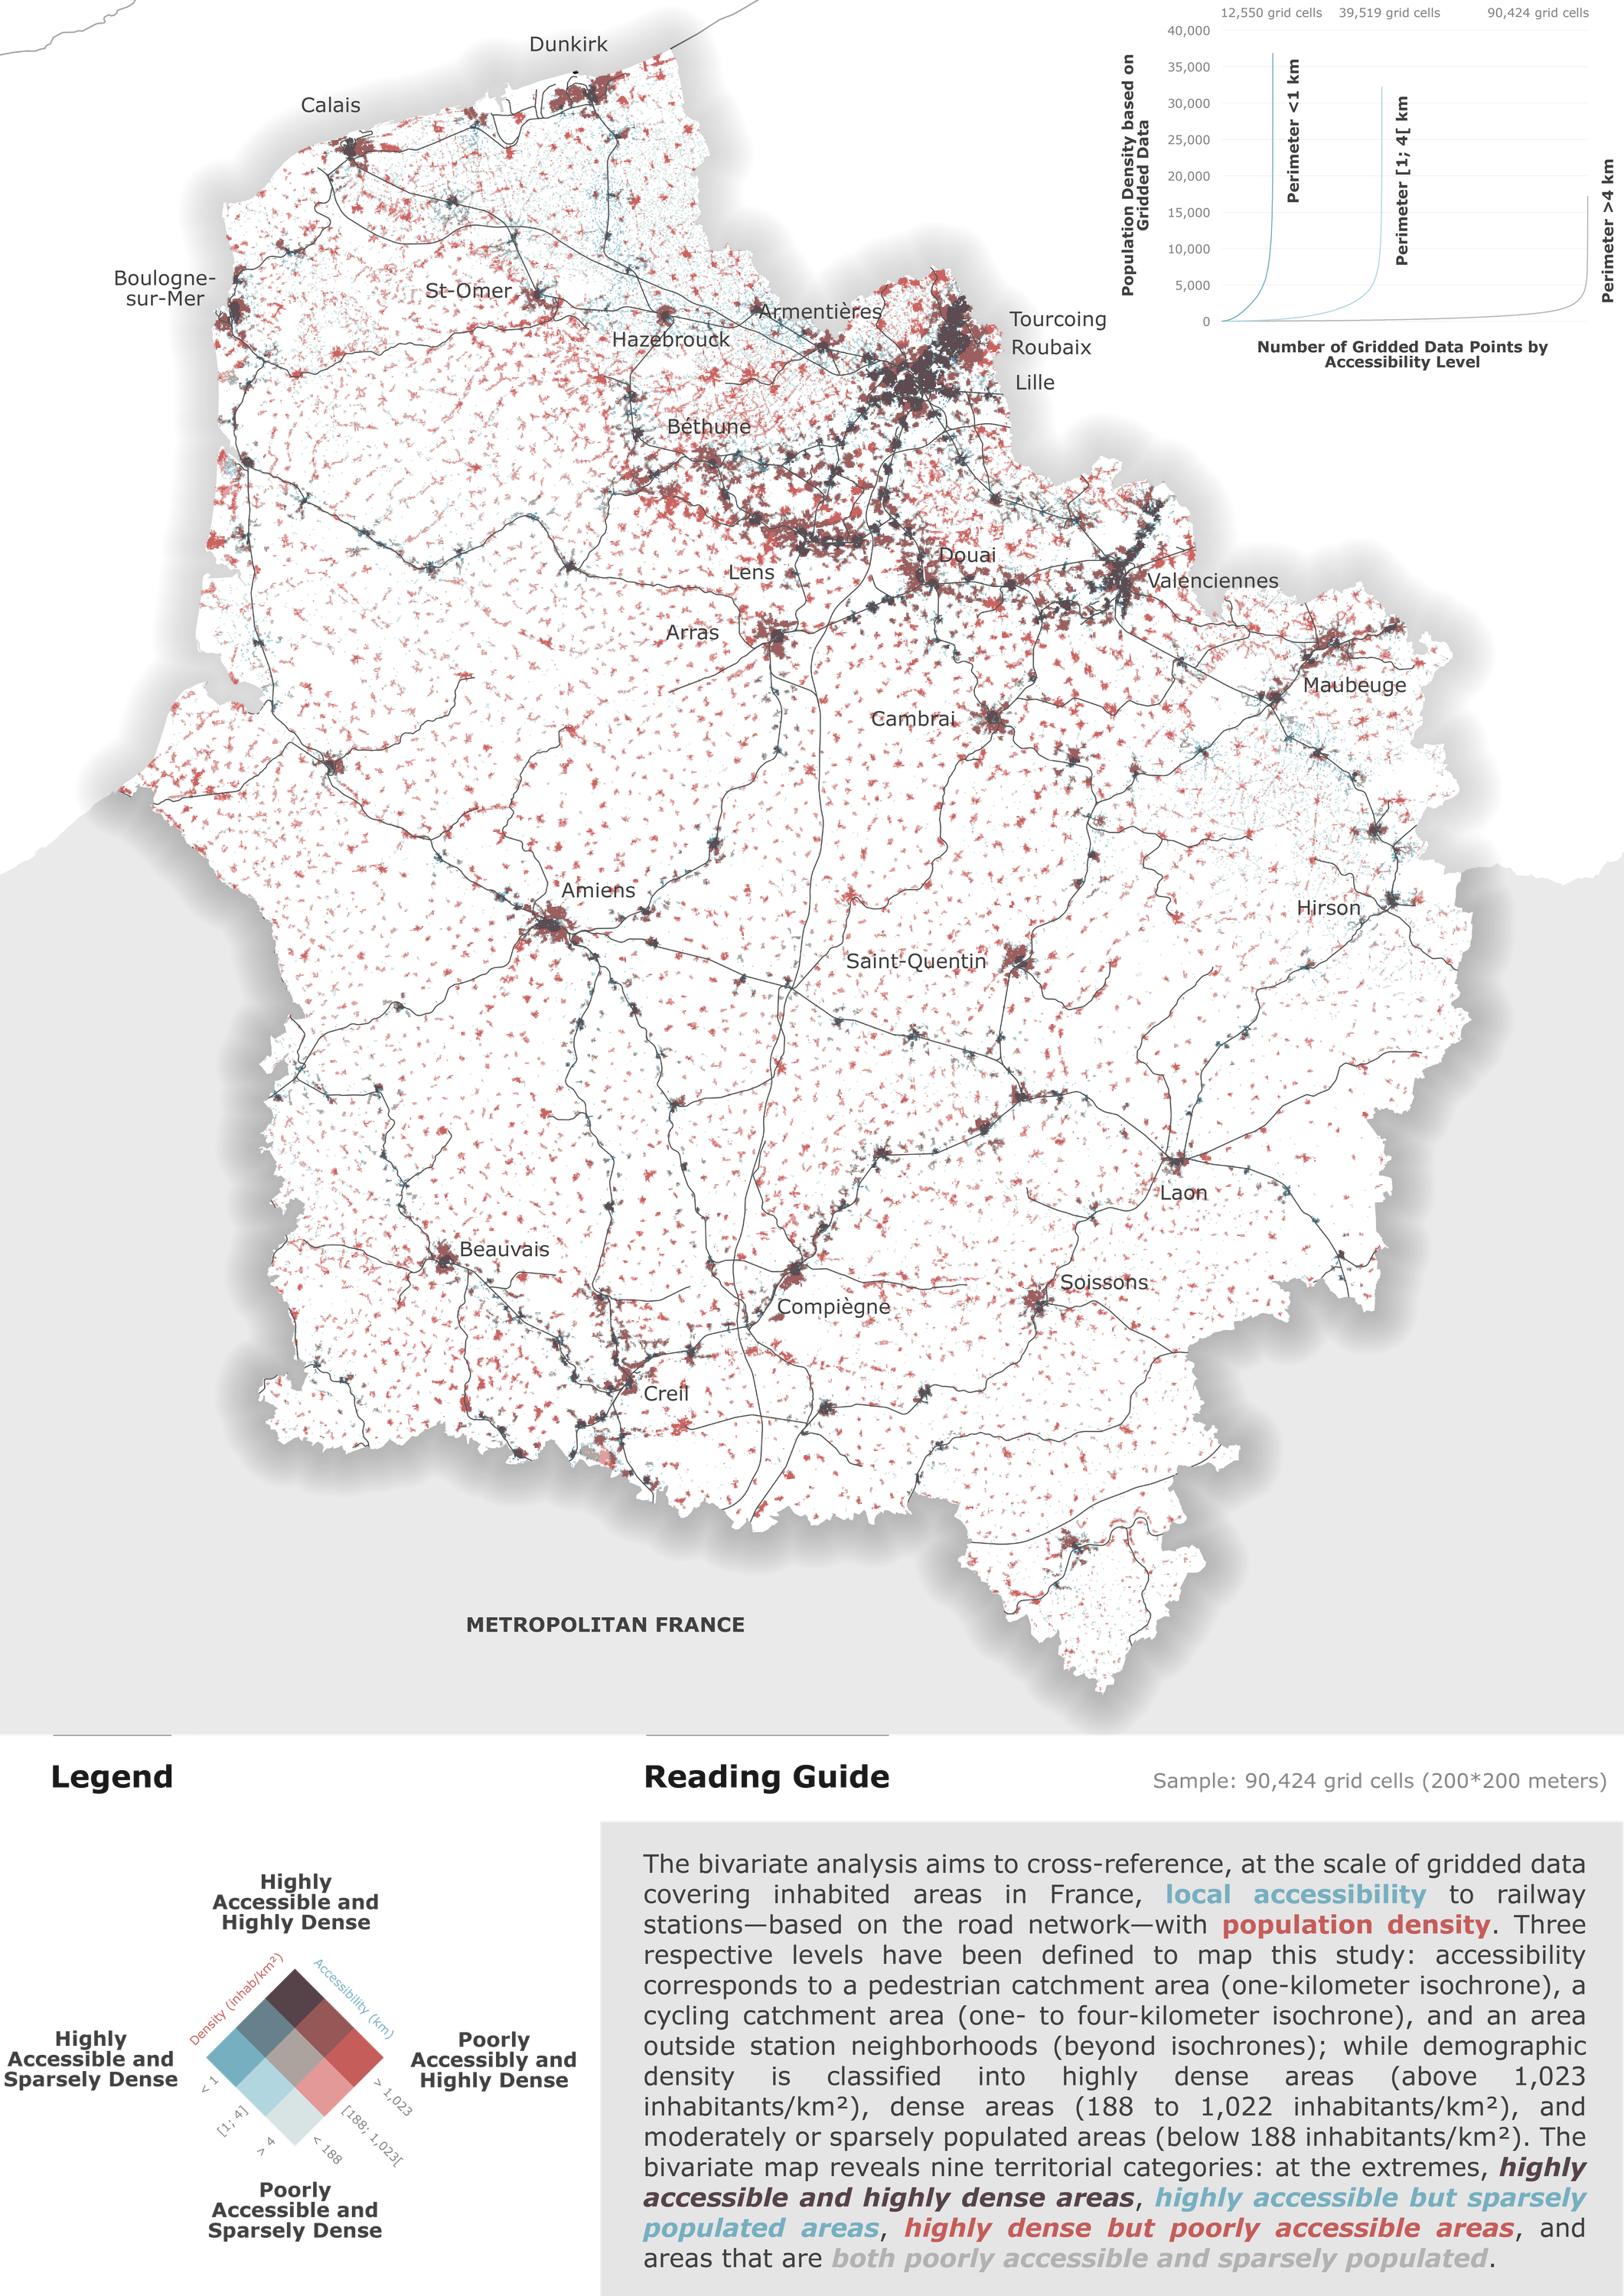
\includegraphics[width=1\columnwidth]{src/Figures/Chap-5/EN_Distances_Carte_bivariee_accessibilite_densite.png}}
        \vspace{5pt}
        \begin{flushright}\scriptsize{
        Sources: Gridded data from \textcolor{blue}{\textcite{insee_grille_2021}}\index{Insee@\textsl{Insee}|pagebf}
        \\
        Author: \textcolor{blue}{Dylan Moinse (2023)}
        }\end{flushright}
    \end{carte}

    % Accessible and dense territories
We can distinguish two forms of cycling accessibility in dense areas: territories benefiting, on one hand, from an urban corridor effect \textcolor{blue}{\autocite[63-65]{liu_corridors_2016}}\index{Liu, Liu|pagebf} structured by railway infrastructure associated with an urban conurbation, and on the other hand, from a ring effect around the central perimeter. Within the \acrfull{MEL}, this includes densely populated municipalities such as Wattrelos, Lys-lez-Lannoy, Hem, and Roncq, located around Roubaix and Tourcoing, as well as Marcq-en-Barœul, Marquette-lez-Lille, Saint-André-lez-Lille, Lambersart, Faches-Thumesnil, Wattignies, Sequedin, Lezennes, and the northern part of Villeneuve d'Ascq around Lille, not forgetting the northern part of Armentières and neighboring municipalities such as La Chapelle-d'Armentières and Nieppe. The Bassin Minier extends significantly when considering cycling isochrones, making densely populated territories such as those in the \acrfull{CABBALR} accessible, including municipalities like Annezin, Beuvry, Fouquereuil, Vaudricourt, Verquin, Verquigneul, Labourse, Lapugnoy, Auchel, Cambrin, Auchy-les-Mines, and certain flow-generating activity zones such as Bruay-la-Buissière or Fouquières-lès-Béthune. The accessible territories within the Communauté d'Agglomération de Lens-Liévin extend to major municipalities such as Liévin, Mazingarbe, Loos-en-Gohelle, Wingles, Pont-à-Vendin, Loison-sous-Lens, Fouquières-lès-Lens, Noyelles-sous-Lens, Méricourt, Rouvroy, and Vimy. The Noyelles-Godault urban and activity zone is fully integrated, as are the peripheral municipalities of Douai, such as Sin-le-Noble, Waziers, and Guesnain, or certain neighboring municipalities of Valenciennes not served by the tram network, like Saint-Saulve, Marly, Douchy-les-Mines, and Raismes. Beyond the \acrshort{MEL} and the Bassin Minier, the bivariate map shows that dense and bike- or micromobility-accessible territories from the stations are mainly the areas surrounding the urban centers of other major cities. Examples include the cities of Grande-Synthe, Leffrinckoucke, and Cappelle-la-Grande in the \acrfull{CUD}, or those of Dainville, Achicourt, Saint-Laurent-Blangy, Saint-Nicolas, and Sainte-Catherine around the Communauté Urbaine d'Arras.%%Translated%%

    % Comparison of tertiary area
Combined walking with the railway network neglects 99.06\% of the regional territory to automobiles, representing 80.48\% of the population. With the introduction of light individual mobility, the accessibility potential allows for a reduction in auto-dependence in these areas, which would affect 92.45\% of the regional territory, but only 44.30\% of the population, or 2,655,929 inhabitants. Furthermore, disregarding physical and anthropogenic barriers, more than 78.46\% of the territory would be classified as automobile-dependent, inhabited by one-third of the population, or 34.60\% (2,074,106 inhabitants).%%Translated%%

    % Implications
These statistical results regarding regional accessibility focused on rail, combined with walking and light individual mobility, first allow us to perceive the strategic challenge of promoting cycling and micromobility by primarily targeting station neighborhoods, in order to offer a sustainable mobility potential to half, or even two-thirds, of the regional population. By adding the structuring role of buses, light individual mobility can significantly contribute to making the alternative mobility system more competitive both at the local level and at the regional and national levels. The second lesson we can draw from this statistical analysis is the identification of an area we can qualify as \Commas{tertiary,} which is considered more dependent on automobiles, and which the reach of light individual mobility cannot cover. Therefore, this analysis also helps to better identify these territories, characterized by a population density much lower than the regional average and station neighborhoods, and then specify more targeted public policies.%%Translated%%

% 5.2.1.3.
\needspace{1\baselineskip} % Reserve space
\subsubsection*{Potential Accessibility Gains primarily Benefiting Disadvantaged Households
    \label{chap5:accessibilite-inclusive}
}

% Introduction
Finally, we focused on improving the potential coverage of the population by the public transport network, with a view to intermodal accessibility aiming for greater inclusivity. To this end, we conducted a geostatistical analysis, examining in more detail the variables associated with the number of social housing units located in the expanded areas around train station neighborhoods. Additionally, this subsection considers the average disposable income of households as well as the real estate values of residential, commercial, industrial, business, and administrative spaces according to pedestrian and cycling zones of influence. This approach allows us to map the interrelations between the socio-economic characteristics of territories and populations and the connectivity provided by public transport infrastructure combined with light individual mobility.%%Translated%%

% Social Housing
The examination of the distribution of social housing in train station neighborhoods, according to their pedestrian and cycling accessibility around stations in the region, is characterized by significant disparities. On the pedestrian scale, the share of social housing is on average 6.53\%, with a median of 5.44\%. In contrast, in areas accessible by bike or micromobility, this proportion increases significantly, reaching an average of 15.85\% and a median of 18.33\%. It is noteworthy that the variance in the share of affordable housing in pedestrian sectors reveals contrasts, with some areas pushing the average higher. At the same time, some train station neighborhoods show a relatively low proportion of social housing, both on the pedestrian and cycling scales. On average, the cycling perimeter records a proportion of social housing that is 2.43 times higher than that of the pedestrian perimeter. This relatively lower presence of social housing in pedestrian station neighborhoods can be attributed to increased real estate pressure in the immediate vicinity of stations, as well as the adoption of urban planning policies favoring other forms of real estate development in these strategic areas. While the immediate surroundings of stations tend to be more densely populated and marked by mixed-use development, cycling-accessible areas offer a more equitable distribution of social housing.%%Translated%%

% Disposable Income
Although train station neighborhoods made accessible through light individual mobility show a significantly higher proportion of social housing, suggesting perspectives for inclusive mobility, the average monthly disposable income per household in these areas is slightly higher than that observed in the areas in direct proximity to the stations. Indeed, the average monthly disposable income per household is~\euro4,217.75 in the \Commas{secondary area}, compared to~\euro4,104.22 in the \Commas{primary area}. Furthermore, the median income in the cycling influence area is~\euro4,172.13, while the median for walking is~\euro4,023.23. This difference reflects an average and median income higher by 2.69\% and 3.57\%, respectively, in the extended train station neighborhoods. However, the last quartile of the income distribution indicates that residents of pedestrian neighborhoods generally earn 9.12\% more, with the income for the third quartile being~\euro4,609.80, compared to~\euro4,224.38 in the bike and micromobility relevant areas. This statistical analysis suggests that the increased presence of students and households consisting of a single active person, who tend to select neighborhoods easily accessible by public transport, contributes to lowering the average income in areas directly near the stations. This observation seems to indicate that it could explain the earlier contradiction between higher income and a larger proportion of social housing in the extended train station neighborhoods.%%Translated%%

% Residential Real Estate Value
Another approach to assess the social inclusivity of areas adjacent to transport hubs is to examine land and real estate values. In this regard, residential real estate values per square meter, relative to housing sale transactions, average~\euro2,138.47 in the pedestrian perimeter, compared to~\euro2,091.54 in the cycling perimeter. Similarly, between 2019 and 2023, 50\% of the homes were sold at a price higher than~\euro1,818.10 per square meter in the pedestrian area, while this threshold was~\euro1,659.96 per square meter in the cycling area, marking a difference of 2.24\% to 9.53\% in favor of the train station neighborhoods accessible by light individual mobility. These data illustrate how the distribution of real estate transactions faces increased land pressure near transport nodes, and how the integration of cycling and micromobility can serve as a tool to mitigate this pressure. This observation can be contextualized through a comparative study of ten Chinese metropolitan areas, published by \textcolor{blue}{\textcite[10]{chu_last_2021}}\index{Chu, Junhong|pagebf}\index{Duan, Yige|pagebf}\index{Yang, Xianling|pagebf}\index{Wang, Li|pagebf}, which shows that the real estate pressure benefited from a gradual decrease in real estate valuation by 4.2\% per kilometer, following the introduction of \acrshort{DBS} services.%%Translated%%
    
% Industrial, Commercial, and Office Real Estate Value + Transition
Regarding real estate transactions in the industrial, commercial, and office sectors, it appears that train station neighborhoods accessible by bike or micromobility exhibit generally significant territorial attractiveness in terms of real estate valuation. We can observe that the average sale price per square meter of industrial, commercial, and office land is~\euro2,480.26 in these areas, compared to~\euro2,072.26 in the pedestrian perimeter of the stations. The median, on the other hand, is~\euro957.97 in the extended train station neighborhoods, compared to~\euro912.26 in the \Commas{primary area.} Unlike the residential sector, the cycling environment around the stations records real estate transactions that are 19.69\% and 5.01\% higher, demonstrating an attractive potential that could encourage the presence of a variety of activities in the same space. In research conducted by \textcolor{blue}{\textcite[10]{zuo_determining_2018}}\index{Zuo, Ting|pagebf}\index{Wei, Hang|pagebf}\index{Rohne, Andrew|pagebf}, it is argued that integrating cycling into the public transport network enables access to over 51\% of disadvantaged households, as opposed to just 27\% for combined walking. This finding highlights the benefits of addressing the \Commas{first and last mile} issue in order to promote more inclusive accessibility. However, the understanding of accessibility should not be limited to evaluating the demographic coverage of the mobility system at the regional scale; it requires a deeper reflection on the accessibility of activity locations that drive movement, such as employment sites and \acrshort{POIs}. The challenge of intermodal accessibility lies not only in considering the place of residence and demographic density but also in the ability to access jobs and strategic destinations within the region.%%Translated%%

% 5.2.2.
\needspace{1\baselineskip} % Reserve space
\subsection{Improvement of Accessibility Potential to Jobs and Destinations via the Public Transport System
    \label{chap5:accessibilite-emplois}
}

% Introduction
In connection with the \acrfull{7Ds}, \textsl{Destination Accessibility} (\(D4\)) should be understood as the ability to access resources and territorial amenities. From this perspective, regional access to job opportunities, as well as to places driving mobility, is a key lever for territorial development and the organization of mobility. It is with this in mind that we will assess the impact of integrating light individual mobility on the accessibility potential to jobs and \acrfull{POIs}.%%Translated%%

% 5.2.2.1.
\needspace{1\baselineskip} % Reserve space
\subsubsection*{Towards a Doubling of Access Potential to Jobs in the Region
    \label{chap5:potentiel-accessibilite-emplois}
}

% Introduction
Building on the \textcolor{blue}{\textcite{repertoire_sirene_des_entreprises_et_de_leurs_etablissements_base_2024}}\index{Sirene@\textsl{Sirene}|pagebf}, a resource made available on March 26, 2024, and updated on May 1, 2024, a geostatistical analysis of job accessibility was made possible, addressing the crucial issue of the \Commas{first and last miles.} By having precise data on the location of businesses and the employment categories within them, our approach involved calculating the average for each employment interval in order to estimate the number of jobs per company. Subsequently, a grid system was established across the entire Hauts-de-France region, using a regular hexagonal arrangement of 1 kilometer, with an apothem of 0.5 kilometers\footnote{~
    This choice of spatial representation, preferred over the traditional square grid, meets accuracy and unnecessary overlap reduction requirements, as hexagons offer better contiguity and uniformity in measuring inter-center distances compared to squares. The apothem of a regular hexagon is the distance from its center to any side of the polygon.
}. Within each hexagon, the total number of jobs varies, with the total value ranging from 0 to 27,175. This spatial structuring was cross-referenced with the generation of pedestrian and cycling isochrones, thus enabling the definition of areas effectively accessible via the public transport system. %%Translated%%

% Statistical Results
The geostatistical analysis revealed, firstly, a notable disparity in access to jobs depending on the size of the territories surrounding the stations. Indeed, pedestrian train station neighborhoods concentrate a total of 1,215,891 jobs, while neighborhoods accessible by bike and micromobility account for 2,135,924 jobs, out of a total of 2,995,421 jobs recorded and located within the regional perimeter. Despite a significantly higher job density in pedestrian-accessible neighborhoods (419 jobs per square kilometer) compared to that of cycling-accessible train station neighborhoods (191 jobs per square kilometer) and a regional average of around 94 jobs per square kilometer, the geographic extent of accessibility differs substantially. As shown in \hyperref[fig-chap5:carte-accessibilite-emplois]{Map~\ref{fig-chap5:carte-accessibilite-emplois}} (page~\pageref{fig-chap5:carte-accessibilite-emplois}), the geographic coverage of walking, coupled with the rail network, amounts to 40.59\% of the total job market, while that of cycling modes stands at 71.31\%. This distribution demonstrates that the integration of light individual mobility, coupled with increased travel speeds, enhances the regional access potential to jobs by 75.67\%.%%Translated%%

% Job Accessibility Map
\begin{carte}[h!]\vspace*{4pt}
    \caption{Map of intermodal accessibility to jobs, supported by the integration of light individual mobility into the rail network, in the Hauts-de-France region.}
    \label{fig-chap5:carte-accessibilite-emplois}
    \centerline{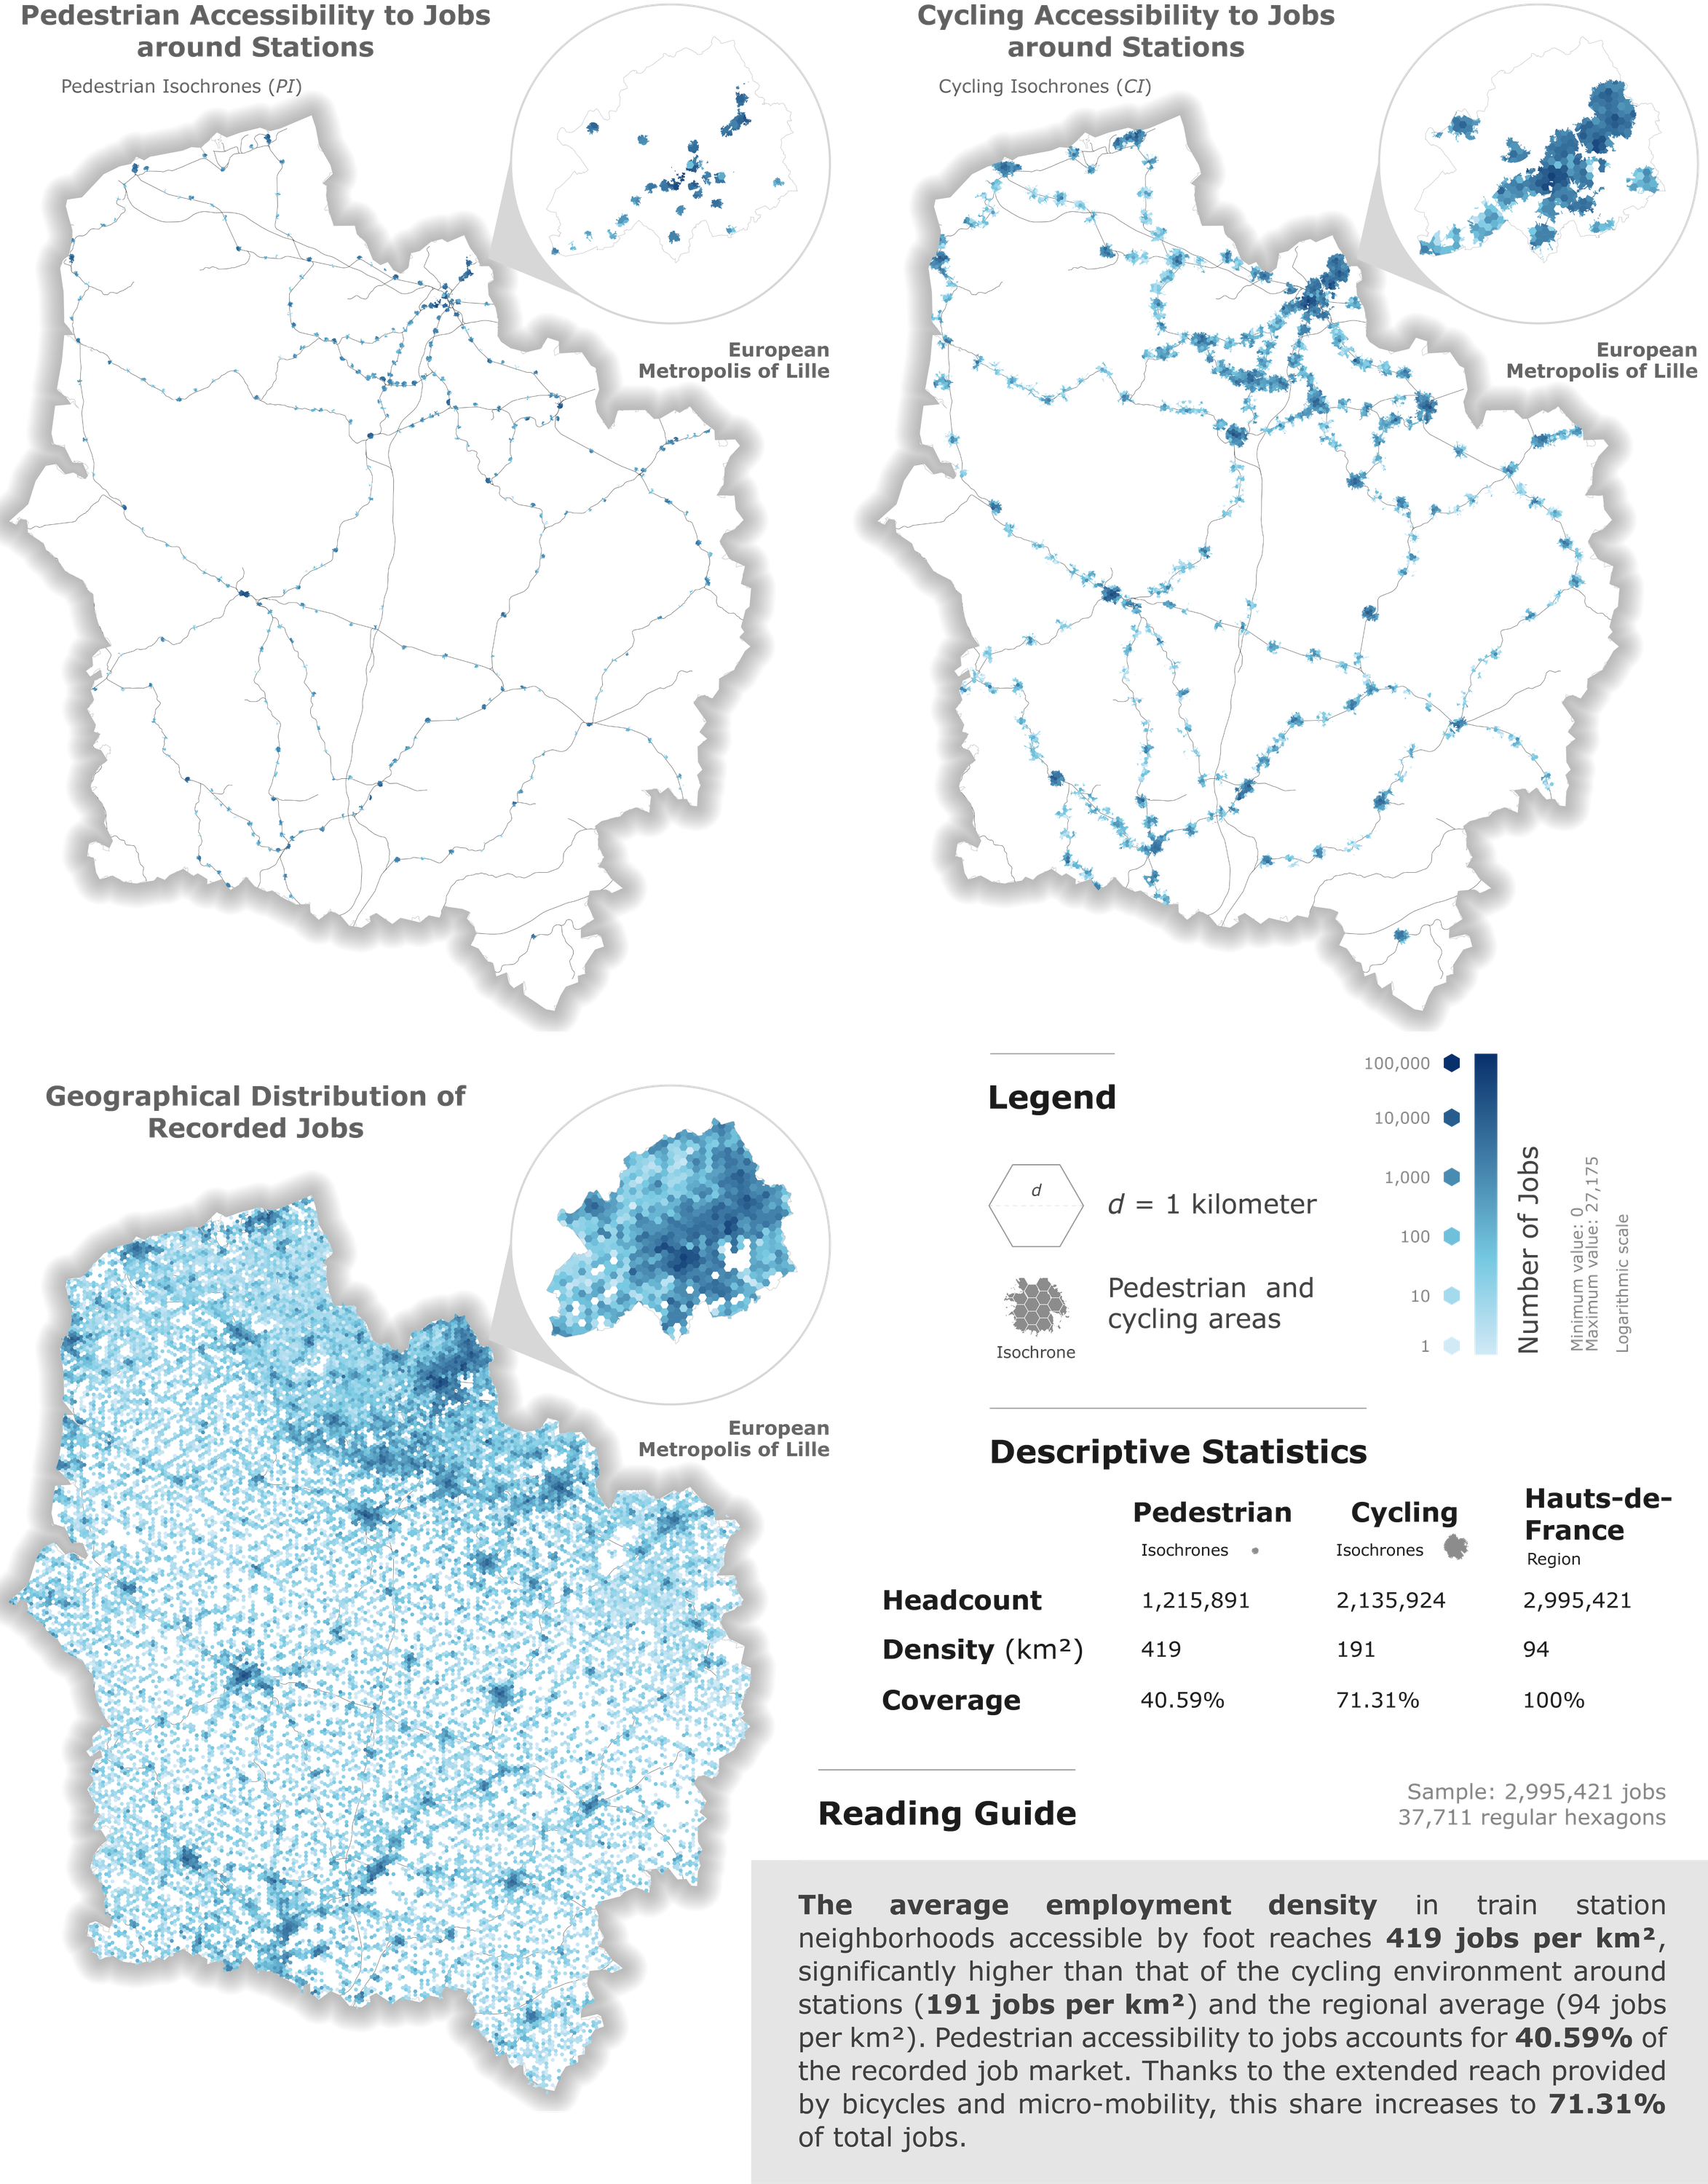
\includegraphics[width=1\columnwidth]{src/Figures/Chap-5/EN_Distances_Carte_emplois.png}}
    \vspace{5pt}
    \begin{flushright}\scriptsize{
    Sources: \textcolor{blue}{\textcite{repertoire_sirene_des_entreprises_et_de_leurs_etablissements_base_2024}}\index{Sirene@\textsl{Sirene}|pagebf}
    \\
    Author: \textcolor{blue}{Dylan Moinse (2024)}
    }\end{flushright}
\end{carte}

% Isochrones and Buffer Differences
By considering the actual accessibility of train station neighborhoods and comparing it to their theoretical area, defined by straight-line radii, our analysis reveals certain disparities. As a result, the number of jobs in pedestrian-accessible train station neighborhoods could increase by 9.94\%, reaching a total of 1,350,027 jobs. Meanwhile, the arean accessible by bike and micromobility would see an increase of 7.99\%, totaling 2,314,215 jobs. Based on Euclidean distances, the extended influence area of the stations could cover up to 77.50\% of jobs at the regional scale. Although the observed differences are not substantial, these statistical variations highlight the need to address the effects of urban cuts more effectively \textcolor{blue}{\autocite[4]{heran_zones_2009}}\index{Héran, Frédéric|pagebf}. In particular, it is essential to better consider physical obstacles and discontinuities such as highways and railways—both within the train station neighborhoods and at the station level, a dead-end issue notably highlighted in the research project \textsl{Bahn.Ville 2} \textcolor{blue}{\autocite[65-67]{lhostis_concevoir_2009}}\index{L'Hostis, Alain|pagebf}\index{Alexandre, Elsa|pagebf}\index{Appert, Manuel|pagebf}\index{Araud-Ruyant, Catherine|pagebf}\index{Basty, Marius|pagebf}\index{Biau, Géraldine|pagebf}\index{Bozzani-Franc, Sandra|pagebf}\index{Boutantin, Gratienne|pagebf}\index{Constantin, Chantal|pagebf}\index{Coralli, Monica|pagebf}\index{Durousset, Marie-Jeanne|pagebf}\index{Fradier, Christophe|pagebf}\index{Gabion, Cyrille|pagebf}\index{Leysens, Thomas|pagebf}\index{Mermoud, Françoise|pagebf}\index{Olny, Xavier|pagebf}\index{Perrin, Emmanuel|pagebf}\index{Robert, Jean|pagebf}\index{Simand, Noémie|pagebf}\index{Stransky, Vaclav|pagebf}\index{Soulas, Claude|pagebf}\index{Verdier, Anne-Marie|pagebf}\index{Vulturescu, Bogdan|pagebf}—or even the urban morphology of the concerned territories, in order to improve job accessibility.%%Translated%%

% Literature
Such insights into the measurement of regional job accessibility gains enabled by these modal combinations have been highlighted in two previous studies. In Hamilton, \textcolor{blue}{\textcite[10]{zuo_first-and-last_2020}}\index{Zuo, Ting|pagebf}\index{Wei, Heng|pagebf}\index{Chen, Na|pagebf}\index{Zhang, Chun|pagebf} demonstrated that the complementarity between cycling and buses leads to a 44\% increase in job accessibility potential, primarily benefiting the most disadvantaged households. In the South Randstad, \textcolor{blue}{\textcite[4-7]{geurs_multi-modal_2016}}\index{Geurs, Karst~T.|pagebf}\index{La Paix Puello, Lissy|pagebf}\index{Weperen, Sander van|pagebf} used the Dutch National Transport Model (NVM) to simulate the effects of six different scenarios on what they call \Commas{destination opportunities} regarding the number of jobs made accessible. The potential for improving access to jobs, through the combination of cycling and the rail network, significantly benefits from public policies that support improvements in cycling routes and parking infrastructure. The analysis of the Leiden-Dordrecht rail corridor reveals that it is primarily the main stations that benefit from these advantages \textcolor{blue}{\autocite[11]{geurs_multi-modal_2016}}\index{Geurs, Karst~T.|pagebf}\index{La Paix Puello, Lissy|pagebf}\index{Weperen, Sander van|pagebf}.%%Translated%%

% 5.2.2.2.
\needspace{1\baselineskip} % Reserve space
\subsubsection*{Towards a Doubling of Access Potential to Destinations in the Region
    \label{chap5:potentiel-accessibilite-destinations}
}

% Introduction
Beyond employment locations, regional access to destinations follows a similar pattern regarding the accessibility gains resulting from the integration of light individual mobility into the rail network. To do this, we relied on the \acrfull{BPE} from \textcolor{blue}{\textcite{insee_base_2021}}, which, after thorough comparisons, proved to be significantly richer, both quantitatively and qualitatively, than the online available mappings. According to \hyperref[table-chap5:accessibilite-poi]{Table~\ref{table-chap5:accessibilite-poi}} (page~\pageref{table-chap5:accessibilite-poi}), the number of \acrshort{POIs} recorded in the train station neighborhoods of the Hauts-de-France region increases from 31,743 to 68,432. This expansion of influence areas has thus allowed for a 2.16-fold increase in access opportunities to \acrshort{POIs}, raising the coverage of destinations from less than a third (30.39\%) to nearly two-thirds (65.52\%). A synthetic interpretation of these descriptive data suggests that the geographical scope of each examined transfer mode provides physical access to one-third of the \acrshort{POIs}: this includes pedestrian and cycling-accessible train station neighborhoods, as well as areas less easily accessible without the use of cars or buses. As a result, the high concentration of \acrshort{POIs} within the train station perimeters compensates for their relatively small area, with a density that is 6.35 times higher than that of less accessible zones.%%Translated%%

    % Tableau accessibilité aux POIs
% Table accessibility to POIs
%%Translated%%
    \begin{table}[h!]
    \centering
    \renewcommand{\arraystretch}{1.5}
    \resizebox{\columnwidth}{!}{
    \begin{tabular}{p{0.35\columnwidth}p{0.12\columnwidth}p{0.17\columnwidth}p{0.12\columnwidth}p{0.12\columnwidth}p{0.12\columnwidth}}
        %\hline
    \rule{0pt}{15pt} \small{\textbf{\textcolor{blue}{Facilities and Services}}} & \small{\textbf{\textcolor{blue}{\textless1 km.}}} & \small{\textbf{\textcolor{blue}{{[}1~;~4{[} km.}}} & \small{\textbf{\textcolor{blue}{\textless4 km.}}} & \small{\textbf{\textcolor{blue}{\geq 4 km.}}} & \small{\textbf{\textcolor{blue}{Region}}}\\
        \hline
    \multicolumn{6}{l}{\textbf{All types of \acrshort{POIs}}}\\
\small{Count} & \small{31,743} & \small{36,689} & \small{68,432} & \small{36,009} & \small{104,441}\\
\small{Share} & \small{30.39\%} & \small{35.13\%} & \small{65.52\%} & \small{34.48\%} & \small{100\%}\\
\small{Density (km\textsuperscript{2})} & \small{63.23} & \small{23.21} & \small{32.87} & \small{9.96} & \small{18.35}\\
        \hdashline
    \multicolumn{6}{l}{\textbf{\acrshort{POIs} of \Commas{proximity}}}\\
\small{Count} & \small{18,976} & \small{23,171} & \small{42,147} & \small{26,371} & \small{68,518}\\
\small{Share} & \small{27.69\%} & \small{33.82\%} & \small{61.51\%} & \small{38.49\%} & \small{100\%}\\
\small{Density (km\textsuperscript{2})} & \small{37.80} & \small{14.66} & \small{20.24} & \small{7.29} & \small{12.04}\\
        \hdashline
    \multicolumn{6}{l}{\textbf{\acrshort{POIs} \Commas{intermediate}}}\\
\small{Count} & \small{9,392} & \small{9,651} & \small{19,043} & \small{7,716} & \small{26,759}\\
\small{Share} & \small{35.10\%} & \small{36.07\%} & \small{71.16\%} & \small{28.84\%} & \small{100\%}\\
\small{Density (km\textsuperscript{2})} & \small{18.71} & \small{6.11} & \small{9.15} & \small{2.13} & \small{4.70}\\
        \hdashline
    \multicolumn{6}{l}{\textbf{\acrshort{POIs} \Commas{superior}}}\\
\small{Count} & \small{3,375} & \small{3,867} & \small{7,242} & \small{1,922} & \small{9,164}\\
\small{Share} & \small{36.83\%} & \small{42.20\%} & \small{79.03\%} & \small{20.97\%} & \small{100\%}\\
\small{Density (km\textsuperscript{2})} & \small{6.72} & \small{2.45} & \small{3.48} &	\small{0.53} & \small{1.61}\\
        \hline
        \end{tabular}}
    \caption{Accessibility to points of interest, centered on train station areas at the reach of pedestrian and cycling levels.}
    \label{table-chap5:accessibilite-poi}
        \vspace{5pt}
        \begin{flushleft}\scriptsize{
        \textcolor{blue}{Note:} The train station districts accessible by bike and micromobility extend up to three kilometers, except for the influence areas of the six multimodal exchange hubs, which have a radius of four kilometers.
        \\
        \textcolor{blue}{Reading Guide:} The \Commas{proximity} and \Commas{intermediate} points of interest are mostly accessible within limited radii, while larger-scale facilities are more concentrated at distances reachable by bike. This highlights a hierarchy of facilities based on their accessibility distance.
        }\end{flushleft}
        \begin{flushright}\scriptsize
        Data sources: \acrfull{BPE} from \textcolor{blue}{\textcite{insee_base_2021}}\index{Insee@\textsl{Insee}|pagebf}
        \\
        Author: \textcolor{blue}{Dylan Moinse (2024)}
        \end{flushright}
        \end{table}%%Rédigé%%

% POI Typology
This geographic analysis of accessibility to \acrshort{POIs} was complemented by a categorization of these points of interest, developed by \textcolor{blue}{\textcite{insee_base_2021}}\index{Insee@\textsl{Insee}|pagebf} based on the type of facility or service associated with each point. The \acrshort{POIs} are then classified into three categories\footnote{~
    \textcolor{blue}{\textcite{insee_base_2021}} provides a typology of facilities based on a framework that considers the sector of activity (for more details, see the updated hierarchical list of facility types in 2021). The dataset consists of 188 facility types:
    \begin{customitemize}
        \item \Commas{Proximity} \acrshort{POIs} include \Commas{services for individuals} (sector \(A\)) such as restaurants, post offices, hair salons, beauty institutes, and real estate agencies; \Commas{commerce} (sector \(B\)) such as grocery stores, bakeries, butcher shops, and florists; \Commas{education} (sector \(C\)) including elementary schools; \Commas{health} (sector \(D\)) such as pharmacies, general practitioners, dentists, and physiotherapists; and \Commas{sports, leisure, and culture} (sector \(F\)) such as libraries and large sports fields, tennis or multi-sport courts;
        \item \Commas{Intermediate} \acrshort{POIs} include \Commas{services for individuals} (sector \(A\)) such as police, gendarmerie, banks, veterinary clinics, and laundromats; \Commas{commerce} (sector \(B\)) such as supermarkets, bookstores, and various types of shops; \Commas{education} (sector \(C\)) including middle schools; \Commas{health} (sector \(D\)) such as medical laboratories, nursing homes, early childhood care facilities, and psychology or speech therapy offices; and \Commas{sports, leisure, and culture} (sector \(F\)) such as swimming pools, skateboarding or cycling parks, and specialized gyms;
        \item \Commas{Superior} \acrshort{POIs} include \Commas{services for individuals} (sector \(A\)) such as local \textsl{France Travail} (formerly \textsl{Pôle emploi}) offices and temporary employment agencies; \Commas{commerce} (sector \(B\)) such as hypermarkets, fishmongers, and perfumeries; \Commas{education} (sector \(C\)) including high schools (general, technological, or professional), universities, and vocational or health training centers; \Commas{health} (sector \(D\)) such as healthcare institutions, psychiatric facilities, specialists, accommodation for children or adults with disabilities, and sheltered employment; and \Commas{sports, leisure, and culture} (sector \(F\)) such as cinemas, cultural exhibitions, and performing arts.
    \end{customitemize}
From the 188 listed facilities in the \acrfull{BPE}, we chose to exclude twelve categories that, in our view, are not relevant to our research topic: automobile and agricultural machinery repair (\(A301\)), automotive technical inspections (\(A302\)), professions of masonry (\(A401\)), plasterer, painter (\(A402\)), carpenter, locksmith (\(A403\)), plumber, roofer, heating technician (\(A404\)), and electrician (\(A405\)), as well as general building companies (\(A406\)), ambulances (\(D303\)), taxis, \acrshort{RHS}\textcolor{blue}{s} (\(E101\)), train stations (\(E107\), \(E108\), and \(E109\)), and sports and health courses (\(F109\)).
}: \Commas{Proximity,} \Commas{Intermediate,} and \Commas{Superior.} The \hyperref[table-chap5:accessibilite-poi]{Table~\ref{table-chap5:accessibilite-poi}} (page~\pageref{table-chap5:accessibilite-poi}), which illustrates the distribution of \acrshort{POIs} based on their proximity to transport hubs, shows a decreasing concentration as the distance from the station increases. However, statistical results reveal that \acrshort{POIs} in the \Commas{Superior} and \Commas{Intermediate} categories are more densely clustered in strategic areas around train stations, while \Commas{Proximity} \acrshort{POIs} are more evenly distributed across the region. Specifically, 79.03\% of superior services are accessible in the extended train station neighborhoods, compared to 71.16\% for intermediate services and 61.51\% for proximity services. In general, expanding the station perimeters has doubled the accessibility to \acrshort{POIs}, with accessibility ratios of 2.03 for intermediate services, 2.15 for superior services, and 2.22 for proximity services.%%Translated%%

% POI Accessibility Map
\begin{carte}[h!]\vspace*{4pt}
    \caption{Map of intermodal accessibility to facilities and services, supported by the integration of light individual mobility into the rail network, in the Hauts-de-France region.}
    \label{fig-chap5:carte-accessibilite-poi}
    \centerline{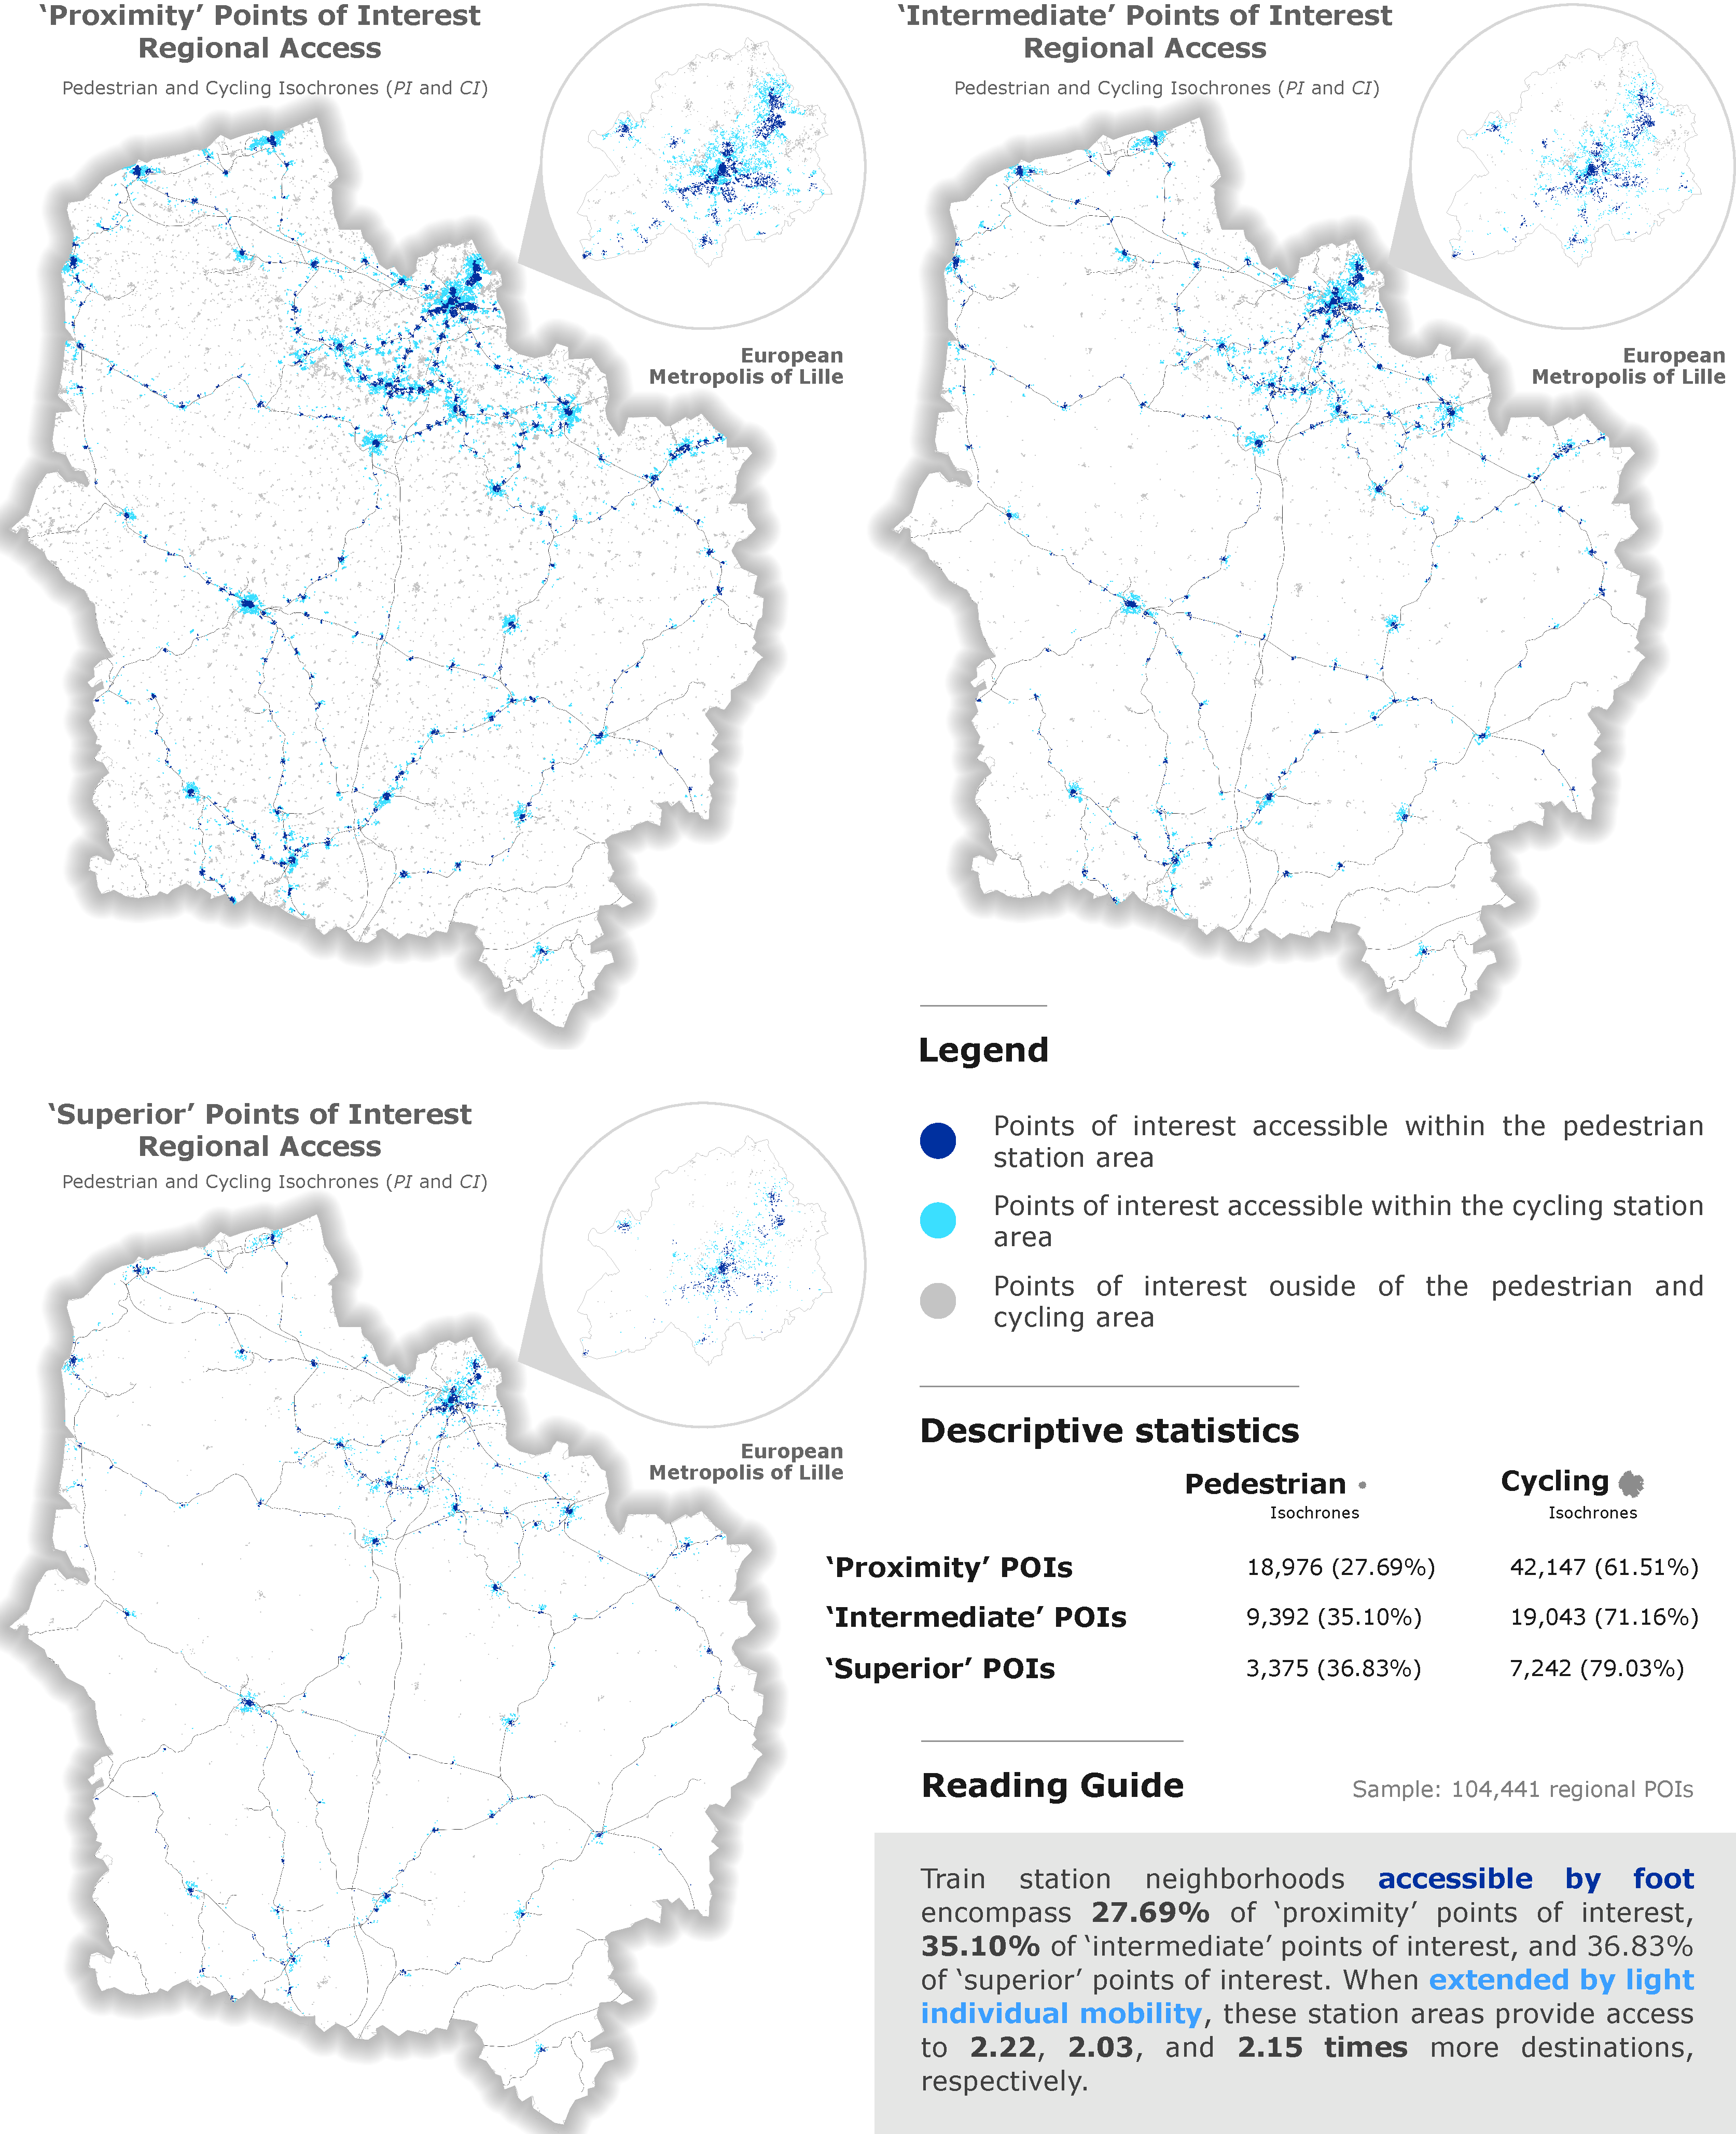
\includegraphics[width=1\columnwidth]{src/Figures/Chap-5/EN_Distances_Carte_POI_compressed.pdf}}
    \vspace{5pt}
    \begin{flushright}\scriptsize{
    Sources: \acrfull{BPE} from \textcolor{blue}{\textcite{insee_base_2021}}\index{Insee@\textsl{Insee}|pagebf}
    \\
    Author: \textcolor{blue}{Dylan Moinse (2024)}
    }\end{flushright}
\end{carte}

% Map Interpretation
The cartographic representation of \acrshort{POIs} in the Hauts-de-France region, presented in \hyperref[fig-chap5:carte-accessibilite-poi]{Map~\ref{fig-chap5:carte-accessibilite-poi}} (page~\pageref{fig-chap5:carte-accessibilite-poi}), allows for visualizing the impact of accessibility gains brought by the integration of light individual mobility into the rail network. This comparative analysis, which includes pedestrian train station neighborhoods, their \Commas{secondary areas,} as well as non-accessible zones, highlights a significant increase in the number of accessible \acrshort{POIs} in restricted spaces, simultaneously revealing a high density of destinations. Furthermore, it is clear that the \acrshort{POIs}, regardless of their category, tend to cluster in a similar manner. Points of interest located beyond the extended train station neighborhoods are mainly discernible at the peripheries of \acrshort{MEL}, the Amiens Metropole Urban Community, and the Mining Basin, especially for superior and intermediate category \acrshort{POIs}. As for proximity \acrshort{POIs}, those located further from the stations are perceived as less essential and would benefit from aligning with population concentrations in the region, in line with the principles of the \Commas{city of short distances} or the \Commas{15-minute city.} This conclusion aligns with the scientific publication by \textcolor{blue}{\textcite[12]{wu_measuring_2019}}\index{Wu, Xueying|pagebf}\index{Lu, Yi|pagebf}\index{Lin, Yaoyu|pagebf}\index{Yang, Yiyang|pagebf}, which emphasizes that access to \acrshort{POIs} related to workplaces and leisure encourages the combined use of bicycles and the subway in Shenzhen, as opposed to residential \acrshort{POIs}, which are more suited to walking.%%Translated%%

% Transition 1
Through the first two sections of this chapter and based on the distribution of the analyzed distances, we were able to determine the size of the train station neighborhoods and thus infer the accessibility gains associated with them. The measurement of distances traveled by users of light individual mobility suggests that a significant portion of these routes exceeds the defined perimeter of the train station neighborhoods. It is important to highlight that this observation raises questions in the context of mobility behaviors characterized by the intermodal use of bicycles or micromobility. The geographic proximity of most public transport stations around the respondents' points of interest should normally encourage them to favor direct routes, thereby minimizing the distance-time and spatial travel. Therefore, this potential tendency to undertake longer trips beyond the \textsl{a priori} optimal distance requires in-depth investigation to attempt to understand the mechanisms and motivations underlying it.%%Translated%%

% Transition 2
It is therefore legitimate to ask the following question: How can we explain that intermodal passengers using bicycles or micromobility might travel a distance greater than the acceptable range for these modes of transportation, when train stations are generally five kilometers apart? In this regard, the following section will address this research question, considering that some of these travelers may bypass nearby public transport network nodes by deliberately taking detours, in order to reduce the perceived costs associated with distance-time or spatial factors, or even due to certain territorial characteristics.%%Translated%%

% ___________________________________________
% 5.3.
\newpage
\needspace{1\baselineskip} % Reserve space
\sectionheader{Optimization of Movement through Detours and Breaks}
\section{Strategies for Optimizing Intermodal Chains through Detours and Breaks
    \label{chap5:detours-pauses-optimisation}
}

% Introduction
In this section, we will explore and analyze in detail certain mobility practices involving detours and breaks within the context of intermodal travel, specifically the use of light individual mobility. It focuses on examining the reasons why some intermodal travelers deliberately choose not to use the nearest public transport stations, opting instead for more distant transport hubs. First, we discuss the \hyperref[chap5:enjeux-detours-pauses]{theoretical framework of detours and breaks} (page~\pageref{chap5:enjeux-detours-pauses}), before proceeding with the \hyperref[chap5:methodes-statistiques]{construction of a sub-sample of trips including breaks and detours} (page~\pageref{chap5:methodes-statistiques}). This is followed by an analysis of these \hyperref[chap5:strategies-optimisation]{spatio-temporal optimization strategies} (page~\pageref{chap5:strategies-optimisation}) and a discussion on the \hyperref[chap5:discussion-detours-pauses-optimisation]{relationship between detours, breaks, and movement optimization} (page~\pageref{chap5:discussion-detours-pauses-optimisation}). This research aims to provide insights into these mobility behaviors, particularly concerning detours and breaks.%%Translated%%

% 5.3.1.
\needspace{1\baselineskip} % Reserve space
\subsection{Theoretical Framework of Detours and Breaks
    \label{chap5:enjeux-detours-pauses}
}

% Introduction
Daily commuting and route choices are often viewed through the lens of efficiency, where the most direct route is assumed to be the most optimal. However, this linear perspective does not account for the mobility strategies employed by users, which incorporate detours and breaks into a complex optimization logic, combining temporal, spatial, and social factors. Far from being mere involuntary deviations from a minimal route, detours can address needs related to accessibility, comfort, safety, or even the qualitative experience of the journey. This approach challenges the traditionally negative connotation associated with detours, viewing them instead as intentional strategies aimed at maximizing travel efficiency.%%Translated%%

% Introduction 2
In this perspective, the concept of \Commas{circuitry} provides a relevant analytical framework to measure these deviations by comparing the actual distance traveled to the Euclidean distance. While the literature tends to consider high circuitry as a limiting factor that reduces the attractiveness of a transport network, certain situations reveal that this metric can also reflect rational trade-offs in favor of smoothness, complex chaining, or the perceived quality of the journey. Thus, studying circuitry in the context of intermodal travel allows for exploring the underlying logics of detours and breaks, whether they are imposed or chosen.%%Translated%%

% 5.3.1.1.
\needspace{1\baselineskip} % Reserve space
\subsubsection*{Detours and Movement Optimization
    \label{chap5:detours-optimisation}
}

% Detour Concept
A physical \gls{detour} is a route that intentionally deviates from the direct trajectory intended to reach a location, typically to bypass material or immaterial obstacles, or to meet specific needs. According to the existing scientific literature surrounding the concepts involved, the detours observed in mobility behaviors would result from a search for spatio-temporal optimization, thus overturning the negative value traditionally associated with detours \textcolor{blue}{\autocite[459]{lhostis_detour_2017}}\index{L'Hostis, Alain|pagebf}. From this perspective, the paths taken by consumers, runners, and tourists, intentionally composed of detours, would be optimal. Each journey within the geographical space would embody a sense of optimality, with geographical distances conforming to this principle \textcolor{blue}{\autocite[2]{lhostis_all_2020}}\index{L'Hostis, Alain|pagebf}. Choices related to detours are therefore associated with the search for multi-factorial optimization, encompassing factors related to the urban environment, physical effort, comfort, activities, personal experience, feelings of safety, and even aesthetic quality.%%Translated%%

% Detour Literature
The literature has primarily explored the detours made by individuals under the influence of the urban environment, such as the treatment of urban forms and public spaces in the San Francisco Bay Area \textcolor{blue}{\autocite[210]{cervero_travel_1997}}\index{Cervero, Robert|pagebf}\index{Kockelman, Kara|pagebf}. Detours have also been documented through the lens of individual factors, such as accompanying children in the Paris metropolitan area \textcolor{blue}{\autocite[149]{motte-baumvol_who_2017}}\index{Motte-Baumvol, Benjamin|pagebf}\index{Bonin, Olivier|pagebf}\index{Belton-Chevallier, Leslie|pagebf}. In the context of light individual mobility, \textcolor{blue}{\textcite[4]{winters_how_2010}}\index{Winters, Meghan|pagebf}\index{Teschke, Kay|pagebf}\index{Grant, Michael|pagebf}\index{Setton, Eleanor~M.|pagebf}\index{Brauer, Michael|pagebf} noted that cyclists tend to take longer routes in Vancouver to access amenities such as green spaces and cycling infrastructure, or to reduce their exposure to the risk of collisions with cars. \textcolor{blue}{\textcite[6]{cubells_e-scooter_2023}}\index{Cubells, Jerònia|pagebf}\index{Miralles-Guasch, Carme|pagebf}\index{Marquet, Oriol|pagebf} highlight the high number of detours made by \acrshort{PeS} users, particularly men, who prefer routes with fewer intersections, in Barcelona. These studies highlight the complexity of detour choices in travel, revealing a diversity of factors influencing these decisions. Detours can be perceived as optimization strategies, subject to the influence of geographic and individual considerations. These observations resonate with an international study conducted by \textcolor{blue}{\textcite[591]{cornet_worthwhile_2022}}\index{Cornet, Yannick|pagebf}\index{Lugano, Giuseppe|pagebf}\index{Georgouli, Christina|pagebf}\index{Milakis, Dimitris|pagebf}, which found that the practice of both conventional and electric cycling, as well as rail and walking modes, stand out for their high levels of satisfaction regarding travel distance-time. In contrast, transfer stages offer only a moderate degree of satisfaction. Moreover, detours can also be attributed to a primarily playful dimension, inherent in \Commas{undirected travel,} which tends to be longer, involve more physical activity, and be positively associated with well-being, as demonstrated by \textcolor{blue}{\textcite[8-9]{hook_undirected_2021}}\index{Hook, Hannah|pagebf}\index{Vos, Jonas de|pagebf}\index{Acker, Veronique van|pagebf}\index{Witlox, Frank|pagebf} in the context of the Flemish region in Belgium.%%Translated%%

% 5.3.1.2.
\needspace{1\baselineskip} % Reserve space
\subsubsection*{Detours and Circuited
    \label{chap5:detours-circuited}
    }

% Negative Circuitry
The analysis of detours can be approached using the circuitry indicator \textcolor{blue}{\autocite[1949]{barrington-leigh_global_2020}}\index{Barrington-Leigh, Christopher|pagebf}\index{Millard-Ball, Adam|pagebf}, which is part of graph theory. Circuitry measures the extent of detours relative to a direct distance, by comparing the shortest path and the Euclidean distance\footnote{~
The Euclidean distance is a measure of the distance between two points in Euclidean space. This geometry corresponds to the square root of the sum of the squares of the differences between the geographic coordinates of the origin and destination points, across a two-dimensional plane (\(x\), \(y\)). For short distances where the curvature of the earth is negligible, the Euclidean distance measures the shortest, \Commas{as-the-crow-flies} path between two points.
}. In the literature, circuitry is generally seen as a constraining element. As a measure intended to assess the attractiveness of travel routes, a low circuitry value indicates fewer detours \textcolor{blue}{\autocite[2]{costa_circuity_2021}}\index{Costa, Miguel|pagebf}\index{Marques, Manuel|pagebf}\index{Moura, Filipe|pagebf}. The circuitry index, viewed in this study as a detour rate, plays a crucial role in evaluating the performance of public transport networks. For example, transport networks with radial line shapes, such as star-shaped, tend to have higher circuitry values for trips from the suburbs, as they require transfers at the core of the network \textcolor{blue}{\autocite[1]{dixit_examining_2021}}\index{Dixit, Malvika|pagebf}\index{Chowdhury, Subeh|pagebf}\index{Cats, Oded|pagebf}\index{Brands, Ties|pagebf}\index{Oort, Niels van|pagebf}\index{Hoogendoorn, Serge|pagebf}. \textcolor{blue}{\textcite[150]{huang_circuity_2015}}\index{Huang, Jie|pagebf}\index{Huang, Jie|pagebf}\index{Levinson, David~M.|pagebf} established a link between higher circuitry and a reduced modal share of public transport in Minneapolis-Saint-Paul, Minnesota. In terms of equity-related issues, an increase in circuitry is correlated with a growing proportion of low-income residents in Amsterdam \textcolor{blue}{\autocite[7]{dixit_examining_2021}}\index{Dixit, Malvika|pagebf}\index{Chowdhury, Subeh|pagebf}\index{Cats, Oded|pagebf}\index{Brands, Ties|pagebf}\index{Oort, Niels van|pagebf}\index{Hoogendoorn, Serge|pagebf}. Regarding light individual mobility, users of traditional bicycles travel, on average, 50\% more spatial distance compared to the Euclidean distance, suggesting limited accessibility for active mobility in various neighborhoods of Lisbon, Portugal \textcolor{blue}{\autocite[13]{costa_circuity_2021}}\index{Costa, Miguel|pagebf}\index{Marques, Manuel|pagebf}\index{Moura, Filipe|pagebf}. At the same time, \textcolor{blue}{\textcite[179]{yen_how_2023}}\index{Yen, Barbara~T.H.|pagebf}\index{Mulley, Corinne|pagebf}\index{Yeh, Chia-Jung|pagebf} demonstrated that circuitry is lower in central districts of Phnom Penh, Cambodia, where the topological and geometric characteristics of the road network are more conducive to walking and cycling.%%Translated%%

% Positive Circuitry
Departing from this negative perspective, the goal of this section is to consider circuitry as a model that can take on a positive connotation, rather than being exclusively viewed as a restrictive factor, as much of the literature might suggest. The most advanced form of detour involves starting a trip in the opposite direction of the final destination in order to reach a more efficient mode of transport, and is defined as \Commas{spatial inversion}\footnote{~
The concept of \Commas{spatial inversion} refers to the approach, whether forced or voluntary, of taking a route that leads in the opposite direction to the intended destination. In the specific context of intermodal transport involving light individual mobility, this geometric detour modality translates into the choice of a converging or diffusing route that takes users toward a direction opposite to that of the origin or destination. As we analyze it in this chapter, spatial inversion can be considered a deliberate strategy aimed at taking advantage of more efficient public transport services, justifying the adoption of detours based on the geometric form.
}~\textcolor{blue}{\autocite[106]{tobler_map_1961, bunge_theoretical_1966}}\index{Tobler, Waldo Rudolph|pagebf}\index{Bunge, William|pagebf}. In this regard, this spatial scheme has been little studied from an optimization perspective. On a national scale, spatial inversion may be seen as restrictive, particularly in the context of the high-speed rail network, which creates a tunnel effect, reducing accessibility to regions between served stations, as shown in the case of the United Kingdom \textcolor{blue}{\autocite[112]{martinez_sanchez-mateos_accessibility_2012}}\index{Martínez Sánchez-Mateos, Héctor~S.|pagebf}\index{Givoni, Moshe|pagebf}. To our knowledge, only two research works have been identified as addressing the concept of circuitry and spatial inversion positively. The first concerns the connection between the \acrfull{HSR} Nord and Paris-Charles de Gaulle Airport \textcolor{blue}{\autocite[144, 161]{lhostis_detour_2014}}\index{L'Hostis, Alain|pagebf}, while the second focuses on the strategic location of the Lesquin secondary train station, aimed at improving intermodal accessibility by bypassing certain detours via the metro from Lille's train stations \textcolor{blue}{\autocite[14-17]{lhostis_definir_2010}}\index{L'Hostis, Alain|pagebf}\index{Conesa, Alexis|pagebf}\index{Arnaud Banos, Thomas Thévenin|pagebf}.%%Translated%%

% 5.3.1.3.
\needspace{1\baselineskip} % Reserve space
\subsubsection*{Breaks and Movement Optimization
    \label{chap5:pauses-optimisation}
    }

% Pauses
In addition to detours, the research that inspires this section and is conducted by \textcolor{blue}{Alain} \textcolor{blue}{\textcite[447]{lhostis_detour_2017}}\index{L'Hostis, Alain|pagebf}, as part of his \acrfull{HDR}, highlights the importance of breaks in optimizing movement. Breaks, defined as periods of immobility during a trip when secondary activities can be undertaken, play a crucial role in resuming ongoing movement. Examples of such breaks include an overnight stay at a hotel to enable long-distance travel, vehicle recharging, or a break on a bench during an urban walk. These breaks are all necessary to generate optimized trips and, similarly to detours, they counterintuitively contribute to the process of optimizing movement and, consequently, distances. Recognizing the role of breaks can lead to reformulating the mathematical definition of geographical distance \textcolor{blue}{\autocite[12]{kloeckner_metrics_2023}}\index{Kloeckner, Benoît|pagebf}. Waiting for a train at a station also constitutes a form of break in movement, made necessary to transition from one network to another. In this regard, selecting a public transport stop to access the public transport system, as well as strategies implemented to avoid an uncomfortable transfer between transport networks or reduce waiting times, result from mobility strategies based on breaks and detours. In this perspective, detours and breaks are interconnected, presenting complex interactions in the formation of trips through a larger optimization process. It is in this context that we propose to apply this concept to the case of light individual mobility integrated into public transport networks, questioning the triptych composed of detours, breaks, and optimization.%%Translated%%

% 5.3.1.4.
\needspace{1\baselineskip} % Reserve space
\subsubsection*{Research Objectives
    \label{chap5:objectifs-recherche}
    }

% Objectifs
This section aims to gain a comprehensive understanding of the route choices and distances traveled by the intermodal travelers considered in this doctoral research, as well as the optimization strategies implemented through the regional case study. The research question presented leads to the formulation of the following sub-hypotheses:
\begin{enumerate}
    \item Users who make detours and/or breaks during their intermodal trips benefit from time and/or spatial distance savings compared to a trip without any detours or pauses;
    \item The identified detours are associated with geometric forms, such as spatial inversion, which, however, do not compromise the spatiotemporal optimization measured;
    \item Detours and breaks vary depending on the characteristics of the intermodal trip. In general, detours are motivated by the desire to avoid transfers within a public transport network, while breaks are primarily used to maximize productivity during a single trip.
\end{enumerate}%%Translated%%
    
% Structure
To address these sub-hypotheses, this section is structured as follows. In the \hyperref[chap5:methodes-statistiques]{subsection on statistical analysis methods} (page~\pageref{chap5:methodes-statistiques}), the applied analytical framework is described, followed by the \hyperref[chap5:strategies-optimisation]{subsection characterization of optimization strategies} (page~\pageref{chap5:strategies-optimisation}), which presents the various results obtained, discussed later in \hyperref[chap5:discussion-detours-pauses-optimisation]{subsection crossed perspectives on detours, breaks, and optimization} (page~\pageref{chap5:discussion-detours-pauses-optimisation}).%%Translated%%

% 5.3.2.
\needspace{1\baselineskip} % Reserve space
\subsection{Statistical Analysis Methods
    \label{chap5:methodes-statistiques}
    }

% Introduction
The optimization of trips relies on a multitude of strategies that go beyond the simple minimization of the distance traveled. In particular, detours, often perceived as inefficient deviations, can actually respond to optimization logics incorporating spatial, temporal, and behavioral constraints. In the context of intermodal mobility, these detours frequently result from the need to access more accessible, better-served public transport infrastructures or those offering better connections. The identification of these detours is based on the Voronoi diagram, a geometric tool that partitions space into influence zones around public transport stations. By comparing the theoretical minimum routes with the actual routes taken, it becomes possible to quantify the prevalence and nature of the detours made. Furthermore, measuring spatiotemporal optimization ratios allows for an evaluation of how these detours contribute to a form of trip optimization, not only in terms of distances traveled but also by incorporating subjective dimensions such as perceived comfort or reduced waiting times. This approach is complemented by a geometric analysis of the angles of intermodal trips, aimed at identifying spatial inversion phenomena, where users deliberately choose to move away from their immediate destination to reach an optimized access point to the transport network. The goal of this section is thus to decipher the underlying optimization logics of detours and breaks in intermodal trips, using spatial geometry tools and metrics for evaluating trip performance.%%Translated%%

% 5.3.2.1.
\needspace{1\baselineskip} % Reserve space
\subsubsection*{Spatial Identification of Detours
    \label{chap5:identification-detours}
    }

% Diagramme de Voronoï
Assuming that cyclists or micromobility users aim to take the shortest route \textcolor{blue}{\autocite[116]{heran_distances_2009}}\index{Héran, Frédéric|pagebf}, an intermodal traveler makes at least one detour when the nearest departure station to the origin or the nearest arrival station to the destination is not used. Once the questionnaire responses have been cleaned, a spatial analysis using a \acrshort{GIS} tool was applied to spatially identify intermodal and commuter trips characterized by one or more detours. To this end, this method uses the visualization of tessellation available in the geometric tools provided in \Marque{QGIS}. The existing rail network, including train, metro, and tram lines as well as public transport stations, was partitioned using the standard Voronoi diagram\footnote{~
The Voronoi diagram, also known as Thiessen polygons, is a geometric representation that divides a space into a series of cells, each associated with a particular data point. These cells are drawn in such a way that every point in a cell is closer to that data point than to any other point in a given space. The result is a partition of space into distinct zones.
} \textcolor{blue}{\autocite[479]{mota_method_2014}}\index{Mota, Diego Rosa|pagebf}\index{Takano, Marise|pagebf}\index{Taco, Pastor Willy Gonzales|pagebf}. In this sense, Voronoi polygons divide the plane into cells from the public transport stations, based on Euclidean measures and independently of the hierarchy of the networks \textcolor{blue}{\autocite[429]{lebedeva_increasing_2018}}\index{Lebedeva, Olga|pagebf}\index{Kripak, Marina|pagebf}\index{Gozbenko, Valeriy|pagebf}.%%Translated%%

%% Map of Flows around Béthune
    \begin{carte}[h!]\vspace*{4pt}
        \caption{Map of flows between origin and destination locations of trips made by respondents corresponding to detours, around the Béthune train station.}
        \label{fig-chap5:flux-origine-destination-detours}
        \centerline{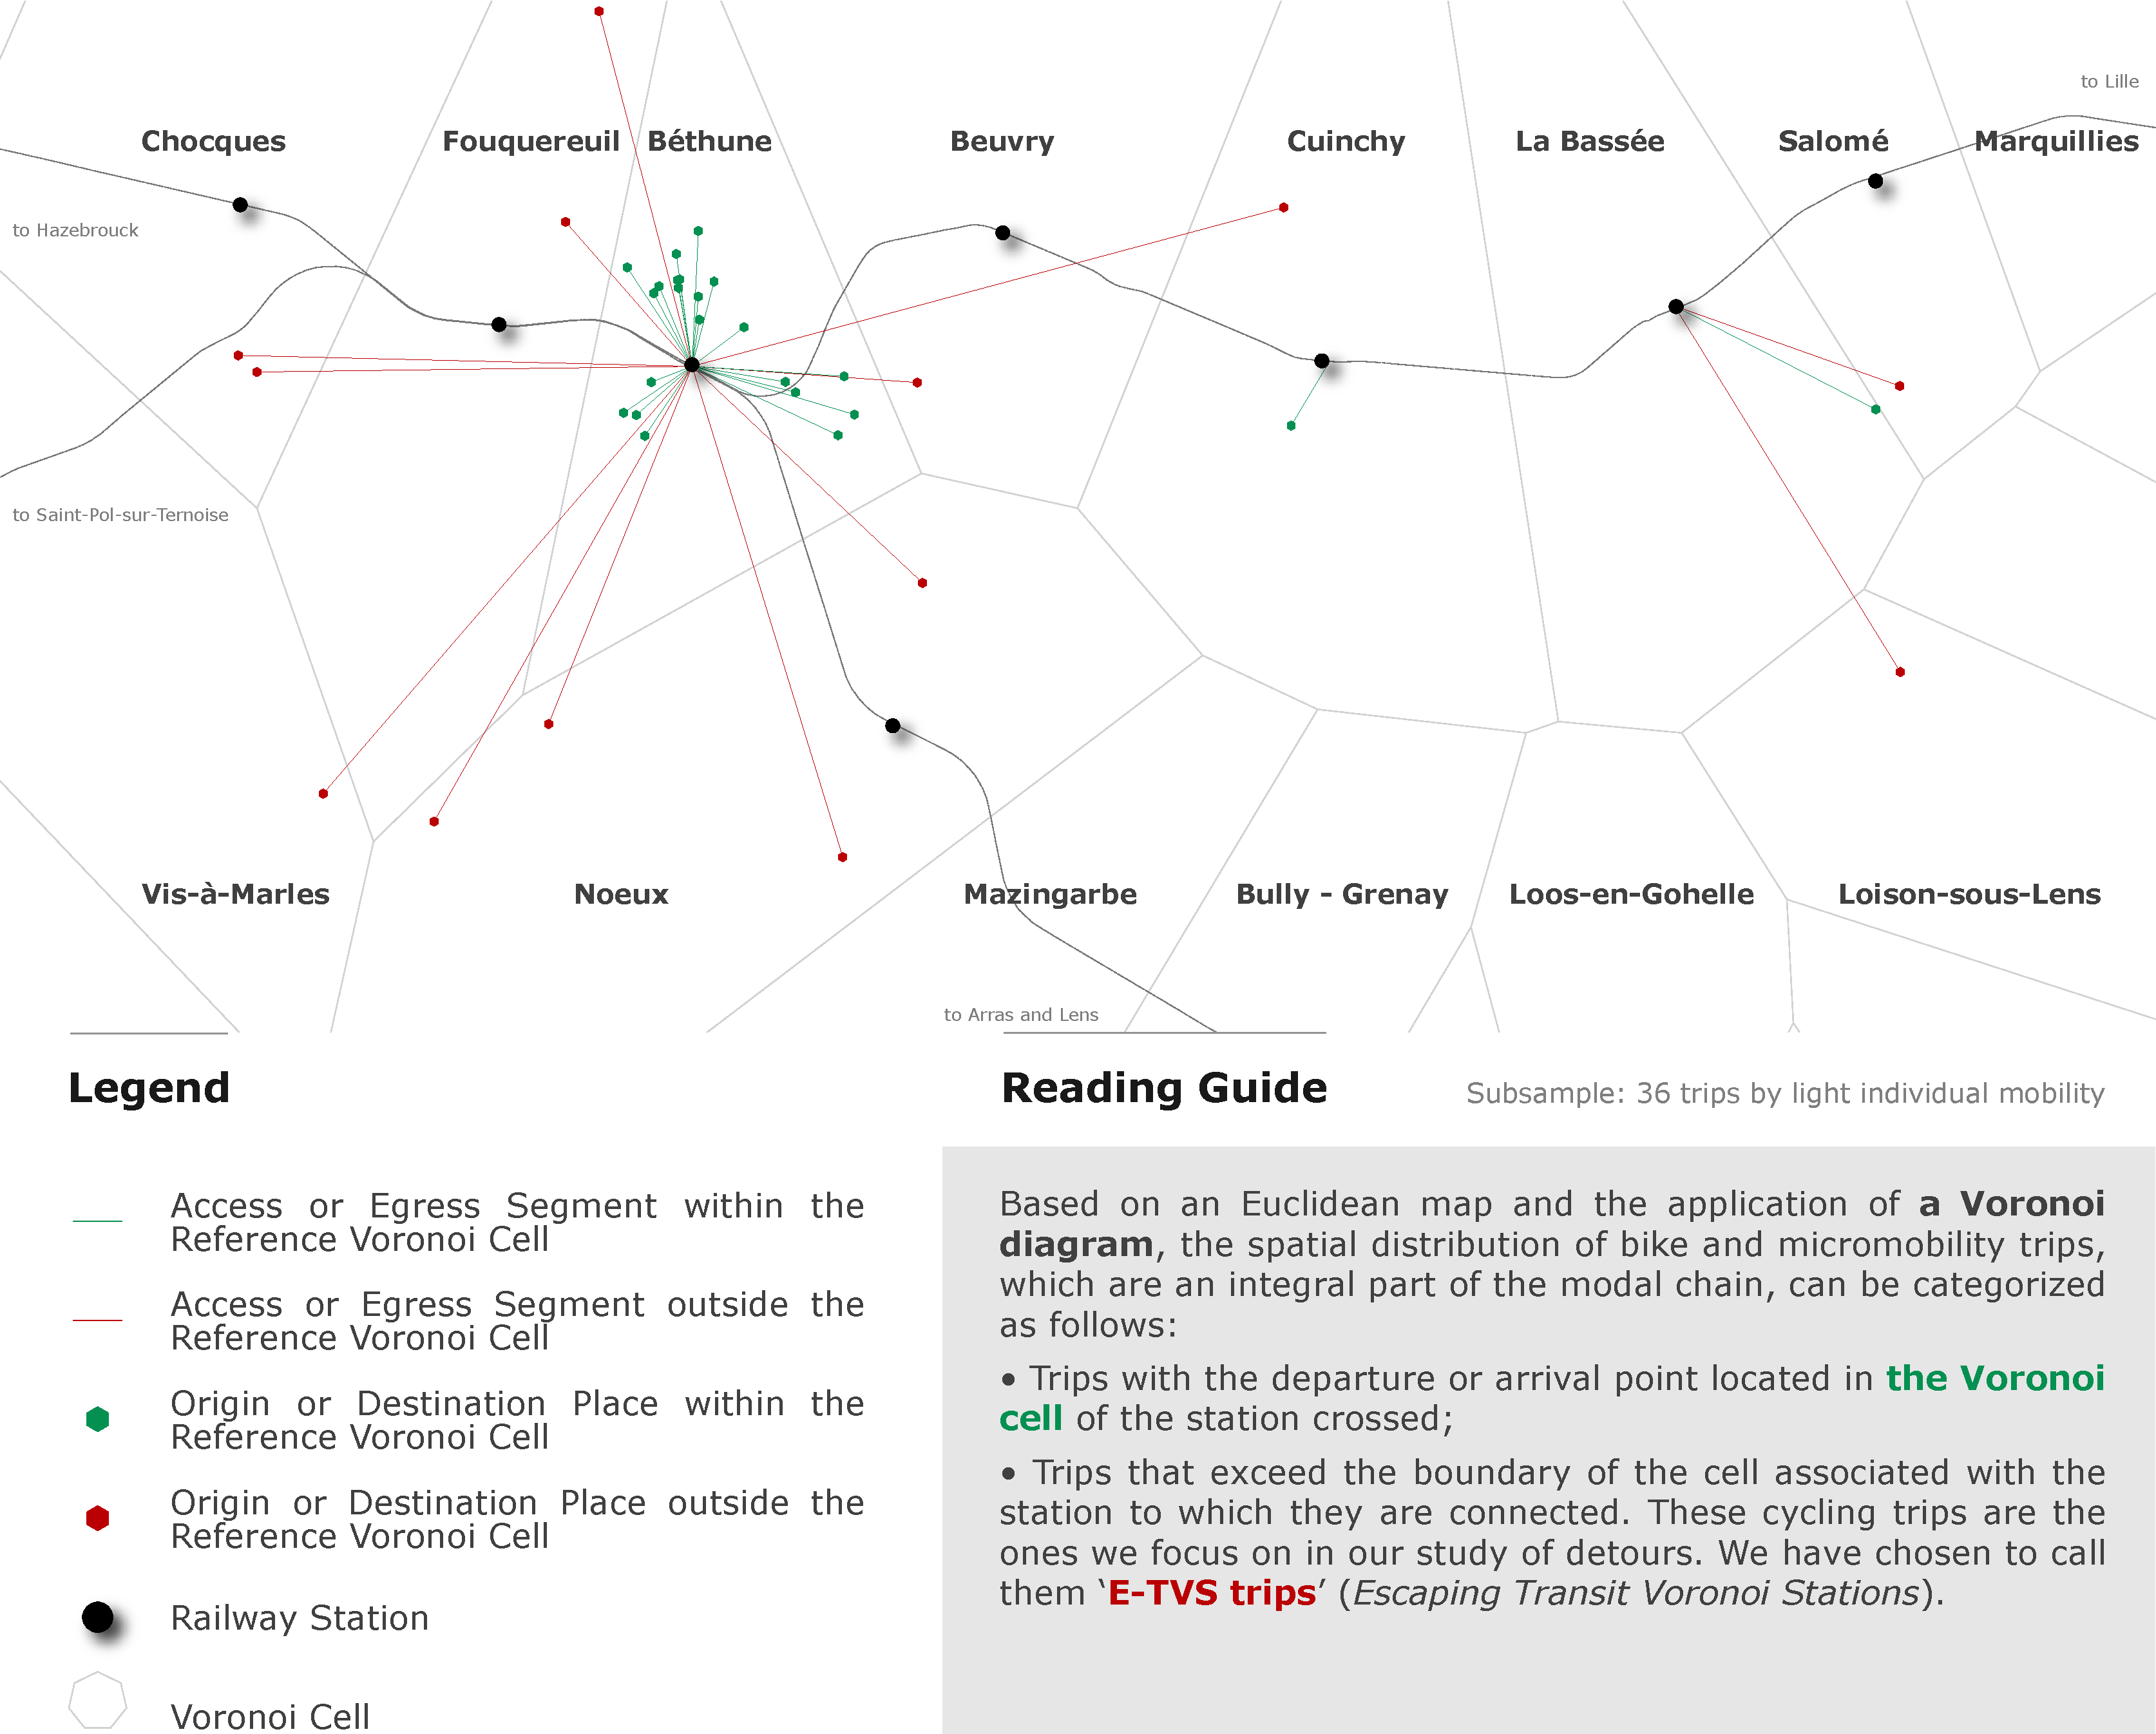
\includegraphics[width=1\columnwidth]{src/Figures/Chap-5/EN_Detours_Diagramme_Voronoi.pdf}}
        \vspace{5pt}
        \begin{flushright}\scriptsize{
        Sources: \acrshort{GTFS} from the \textsl{Open Data} of \textcolor{blue}{\textcite{sncf_sncf_2022}}\index{SNCF@\textsl{SNCF}|pagebf} and \textcolor{blue}{\textcite{metropole_europeenne_de_lille_opendata_2021}}\index{Métropole Européenne de Lille@\textsl{Métropole Européenne de Lille}|pagebf}
        \\
        Author: \textcolor{blue}{Dylan Moinse (2023)}
        }\end{flushright}
    \end{carte}

% E-TVS
The production of such a technique led to the cartographic visualization shown on \hyperref[fig-chap5:flux-origine-destination-detours]{Map~\ref{fig-chap5:flux-origine-destination-detours}} (page~\pageref{fig-chap5:flux-origine-destination-detours}). This type of cartographic representation then takes the form of a simplified Voronoi diagram focused on the public transport network (\textsl{Simplified Transit Voronoi Diagram}, T-VD), conceptualized by \textcolor{blue}{\textcite[5]{chen_transit_2022}}\index{Chen, Jieh-Haur|pagebf}\index{Teng, Wenxin|pagebf}\index{Jia, Tao|pagebf}\index{Chen, Hui-Ping|pagebf}\index{Liu, Xianglong|pagebf} and designed to assign the theoretically nearest station to each origin and destination point.%%Translated%%

% Cette analyse cartographique a été améliorée à l'aide de l'utilisation de la transparence des couleurs afin de mettre en relief les matrices de flux symétriques. En effet, l'efficacité de la transparence combinée à un fond noir réside dans l'amélioration de la \Commas{saillance visuelle}\footnote{~
% La notion de \Commas{saillance visuelle}~se réfère à l'adéquation entre le phénomène représenté, les variables visuelles mobilisées et sa perception par l'observateur·rice.
% } des figurés et des informations ainsi que dans la facilitation de la perception des flux de faible valeur tout en garantissant une certaine lisibilité, comme explicité dans la thèse de doctorat de \textcolor{blue}{\textcite[226]{bahoken_contribution_2016}}\index{Bahoken, Françoise|pagebf} sur la cartographie d’une matrice de flux. 

% 5.3.2.2.
\needspace{1\baselineskip} % Reserve space
\subsubsection*{Sampling Process
    \label{chap5:echantillonnage-detours-pauses}
    }

% Echantillonnage
To create sub-samples focused on detours and breaks (see \hyperref[fig-chap5:echantillonnage-detours-pauses]{Figure~\ref{fig-chap5:echantillonnage-detours-pauses}}, page~\pageref{fig-chap5:echantillonnage-detours-pauses}), the sampling process captured complete responses (\textsl{exclusions 1 and 2}), including the last intermodal trip (\textsl{exclusion 3}), providing valid geographic coordinates (\textsl{exclusion 4}), with a converging and/or diffusing trip made by bicycle or micromobility and characterized by an identified detour or a declared break (\textsl{exclusion 5}), and having a trip purpose related to work or study (\textsl{exclusion 6}). It should be noted that the definition of a detour used in this study corresponds to the use of a public transport station different from the nearest one to the origin or destination. The detour-based sample includes 129 intermodal trips, while the pause-based sample consists of 110 responses. It is important to highlight that intermodal trips involving one or more detours and/or one or more breaks represent 59\% and 51\% of the eligible trips, respectively. The spatial identification of trips marked by the presence of detours specifically resulted in a list of 171 converging and diffusing trips involving a detour using light individual mobility, suggesting that some travelers make multiple detours during a single trip. Among the intermodal travelers who made a detour (129 trips) and reported a break (110 trips), 73 of them combined both practices. Specifically, 59 of them opted for a break and a detour to access a public transport station, while 42 did so to leave it. Additionally, 28 of these travelers combined a break and a detour at both the first and last kilometers of their trip.%%Translated%%

%% Figure sampling detours and pauses
    \begin{figure}[h!]\vspace*{4pt}
        \caption{Sampling process based on identified detours and declared breaks in the administered questionnaire.}
        \label{fig-chap5:echantillonnage-detours-pauses}
        \centerline{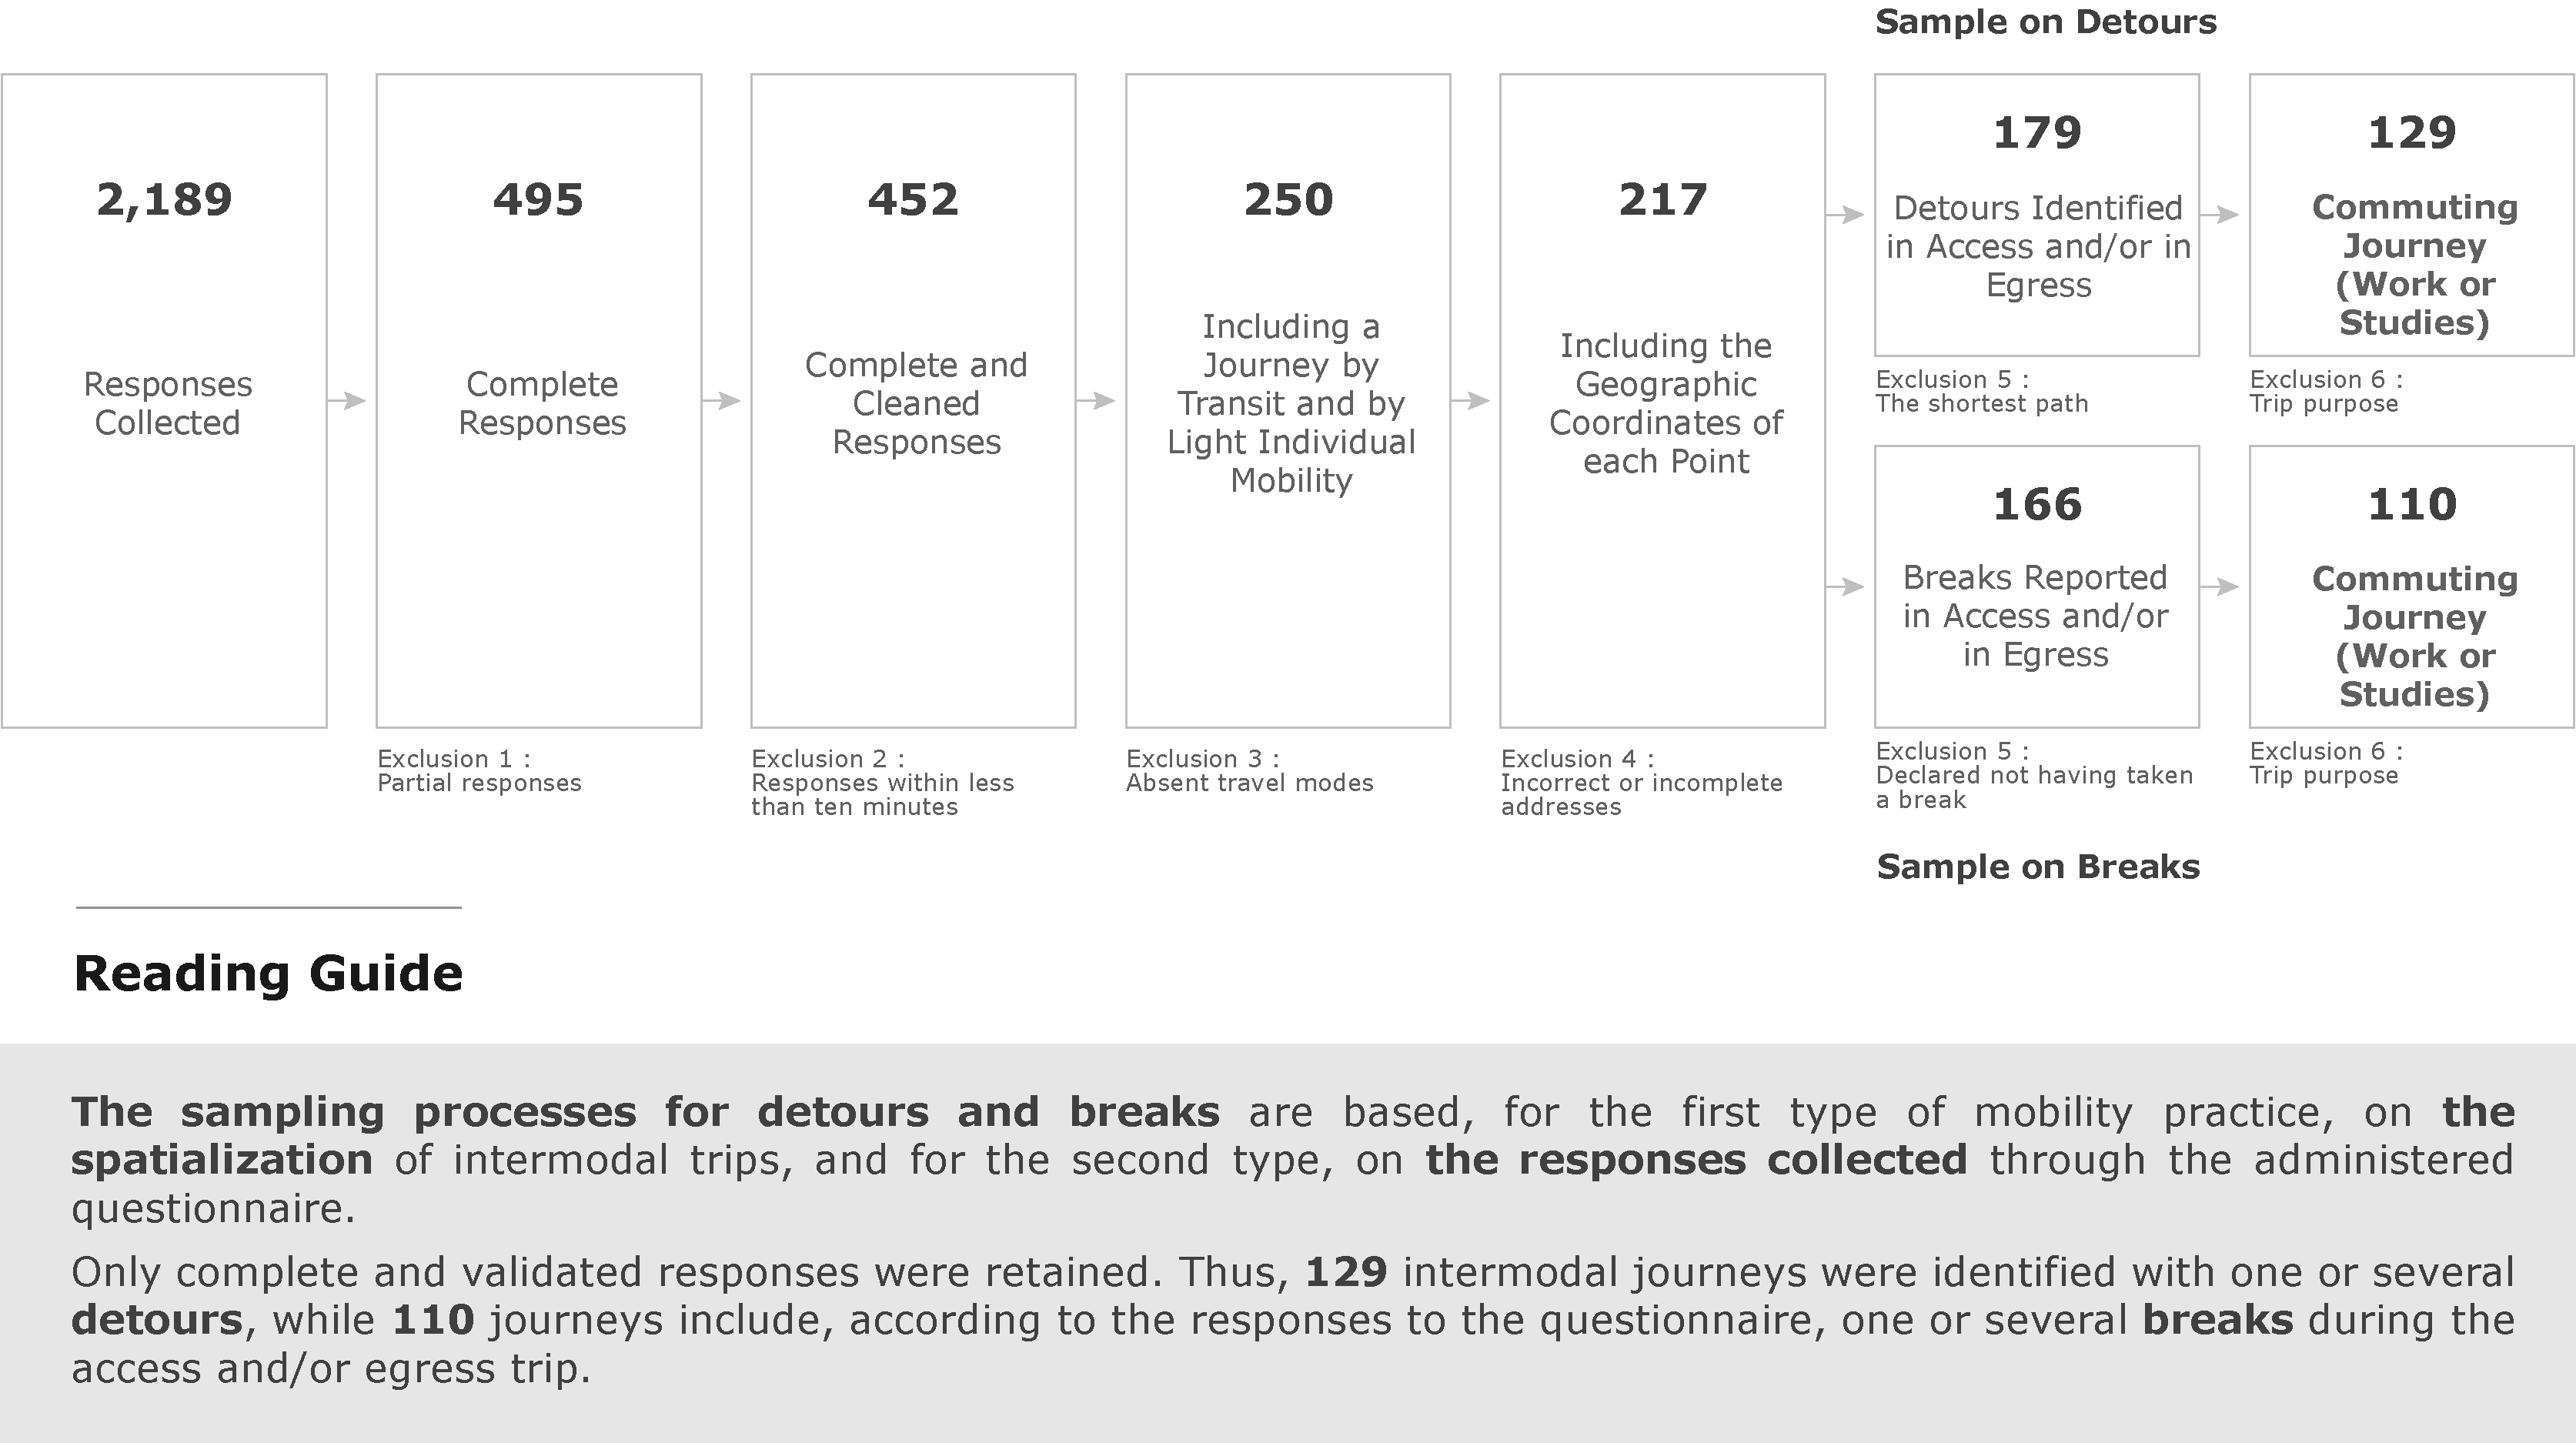
\includegraphics[width=1\columnwidth]{src/Figures/Chap-5/EN_Detours_Echantillonnage.pdf}}
        \vspace{5pt}
        \begin{flushright}\scriptsize{
        Author: \textcolor{blue}{Dylan Moinse (2023)}
        }\end{flushright}
    \end{figure}

% E-TVS
By entering the 217 validated geographic coordinates associated with the origin and destination locations linked to the public transport stations used, 129 trips emerged as having one or more stations not corresponding to the reference Voronoi cell. Among the 129 identified routes, 83 of them took place in the Hauts-de-France region. We have named this type of trip, which involves at least one detour, integrated into an \gls{intermodality} context, a \Commas{public transport station escaping the Voronoi cell} (\acrfull{E-TVS}).%%Translated%%

% Detours and breaks simultaneously
Among the studied population of intermodal travelers who both made a detour (129 trips) and took a break (110 trips), it appears that 73 individuals integrated both activities simultaneously. More specifically, 59 of these travelers made a detour and took a break during the access stage, compared to 42 of them in the egress stage, while 28 travelers made a detour and took a break at both ends of the trip.%%Translated%%

% 5.3.2.3.
\needspace{1\baselineskip} % Reserve space
\subsubsection*{Measurement of Spatiotemporal Optimization Ratios
    \label{chap5:calcul-ratio-optimisation}
}

% Actual and Alternative
Two different types of trips were mapped on \Marque{QGIS}~by importing the routes provided by the trip planner \Marque{Graphhopper}. The first is the estimated actual trip (\(eff\)), which corresponds to the shortest route from the network and actually traveled by the respondent, and which includes a \acrshort{E-TVS} trip. The second represents a hypothetical alternative trip scenario (\(alt\)), in which the individual accesses the nearest public transport station with the shortest spatial distance. The actual routes are measured in terms of effective spatial distance\footnote{~
    According to \textcolor{blue}{\textcite[308]{deutsch_note_1961}}\index{Deutsch, Karl~W.|pagebf}\index{Isard, Walter|pagebf}, \Commas{effective distance} cannot simply be measured in terms of spatial distance between two points, entities, or individuals. This concept embraces a multidimensional view of distance related to a journey, which is the product of physical distances, economic (costs), social (quantity and nature of interactions), and communication-related (efficiency and frequency of exchanges). Other factors may further influence the measurement of effective distance.
} estimated (\(km_{eff}\)) \textcolor{blue}{\autocite[34]{cauvin-reymond_perception_1984}}\index{Cauvin-Reymond, Colette|pagebf}, reflecting the balance between objective distances \textcolor{blue}{\autocite{brigss_methodologies_1976}}\index{Brigss, Ronald|pagebf} and cognitive, subjective, and perceived distances \textcolor{blue}{\autocite{canter_psychology_1977, bailly_perception_1977, sadalla_perception_1980}}\index{Canter, David~V.|pagebf}\index{Bailly, Antoine|pagebf}\index{Sadalla, Edward~K.|pagebf}\index{Magel, Stephen~G.|pagebf}, as well as effective distance-time values (\(t_{eff}\)), whether objective (\(t_{eff_{(O)}}\)) or perceived (\(t_{eff_{(P)}}\)). Similarly, the alternative trip is described by spatial distance parameters (\(km_{alt}\)) and alternative distance-time (\(t_{alt_{(O)}}\) and \(t_{alt_{(P)}}\)), as shown in \hyperref[equation-chap5:effectif-alternatif]{Formulas~\ref{equation-chap5:effectif-alternatif}} (page~\pageref{equation-chap5:effectif-alternatif}) below:%%Translated%%

\begin{equation}
\label{equation-chap5:effectif-alternatif}
\begin{array}{lclclclclclcl}
\displaystyle km_{alt} = km_{R(alt)} + km_{TC(alt)} + km_{D(alt)}\\\\
\displaystyle km_{eff} = km_{R(eff)} + km_{TC(eff)} + km_{D(eff)}\\\\
\displaystyle t_{alt_O} = t_{R(alt_O)} + t_{TC(alt_O)} + t_{D(alt_O)}\\\\
\displaystyle t_{eff_O} = t_{R(eff_O)} + t_{TC(eff_O)} + t_{D(eff_O)}\\\\
\displaystyle t_{alt_P} = 1.8*t_{R(alt_P)} + 2.8*t_{A(alt_P)} + 1*t_{TC(alt_P)} + 1.8*t_{D(alt_P)}\\\\
\displaystyle t_{eff_P} = 1.8*t_{R(eff_P)} + 2.8*t_{A(eff_P)} + 1*t_{TC(eff_P)} + 1.8*t_{D(eff_P)}
\end{array}
\end{equation}

\begin{align*}
    &\text{where:} \\
    _R &\text{ represents the feeder trip to the station;} \\
    _D &\text{ represents the distribution trip from the station;} \\
    _{TC} &\text{ represents the public transport trip(s);} \\
    _A &\text{ represents the waiting time during a transfer.}
\end{align*}

% Explanation of the equation
Since \(t_{eff_{(P)}}\) and \(t_{alt_{(P)}}\) are measured using specific weightings for each component of the trip, namely the feeder and distribution trips, as well as the waiting time, which respectively have a perceived time value 1.8 times higher \textcolor{blue}{\autocite[110]{wardman_review_2001, gleave_transport_1997}}\index{Wardman, Mark|pagebf}\index{Gleave, Steer Davies|pagebf} and 2.8 times higher \textcolor{blue}{\autocite[110]{horl_introducing_2021, wardman_review_2001}}\index{Hörl, Sebastian|pagebf}\index{Balac, Milos|pagebf}\index{Wardman, Mark|pagebf} compared to the onboard time of the main public transport mode. This multiplication of time more realistically integrates the waiting time and travel time by bike or micromobility into the perceived time formula. The waiting time required for a public transport mode is estimated based on peak hours for these commuting or study-related trips and varies depending on the type of public transport used. A precautionary time of fifteen minutes is assumed for the \acrshort{HST} and Intercité \textcolor{blue}{\autocite[12]{pagliara_high-speed_2012}}\index{Pagliara, Francesca|pagebf}\index{Vassallo, José Manuel|pagebf}\index{Román, Concepción|pagebf}, ten minutes for the \acrshort{TER} and Transilien \textcolor{blue}{\autocite[300]{ingvardson_passenger_2018}}\index{Ingvardson, Jesper Bláfoss|pagebf}\index{Nielsen, Otto Anker|pagebf}\index{Raveau, Sebastián|pagebf}\index{Nielsen, Bo Friis|pagebf}, and five minutes for the \acrshort{RER}, metro, and tramway \textcolor{blue}{\autocite[300]{hua_comprehensive_2018, ingvardson_passenger_2018}}\index{Hua, Weixin|pagebf}\index{Feng, Xuesong|pagebf}\index{Zhu, Xiaojing|pagebf}\index{Jie, Yuanpeng|pagebf}\index{Ingvardson, Jesper Bláfoss|pagebf}\index{Nielsen, Otto Anker|pagebf}\index{Raveau, Sebastián|pagebf}\index{Nielsen, Bo Friis|pagebf}.%%Translated%%

% Ratios
The level of detour was measured based on the ratio between the actual route (\(eff\)) and its spatial distance compared to a detour-free route (\(alt\)) and the Euclidean distance (\(eud\)). These two ratios are used in the scientific literature, the first referred to as the \acrfull{RDI}, or Route Directivity Index, which measures connectivity relative to the Euclidean distance \textcolor{blue}{\autocite[193]{park_why_2019}}\index{Park, Yujin|pagebf}\index{Akar, Gulsah|pagebf}, and the second as the \acrfull{GRDI}, or Geographic Route Directivity Index, relative to the shortest path on a network \textcolor{blue}{\autocite[126]{ciscal-terry_analysis_2016}}\index{Ciscal-Terry, Wilner|pagebf}\index{Dell'Amico, Mauro|pagebf}\index{Hadjidimitriou, Natalia Selini|pagebf}\index{Iori, Manuel|pagebf}. In the context of this research, which aims to revisit detours as a means to optimize travel in a spatiotemporal manner, the indicator originally intended to calculate the circuit rate (\acrshort{GRDI}) was inverted to capture the differences resulting from detours. We thus named the \acrshort{GRDI} adapted to our study the \Commas{Optimization Ratio,} denoted as \(R\). The optimization rate is defined in spatial distance (\(R_{km}\)) and distance-time, broken down into objective time (\(R_{t{(O)}}\)) and perceived time (\(R_{t_{(P)}}\)), as expressed in \hyperref[equation-chap5:ratios-optimisation]{Formulas~\ref{equation-chap5:ratios-optimisation}} (page~\pageref{equation-chap5:ratios-optimisation}).%%Translated%%

\begin{equation}
\label{equation-chap5:ratios-optimisation}
\begin{array}{lclcl}
\displaystyle R_{km} = \displaystyle\frac{km_{alt}}{km_{eff}}\\\\
\displaystyle R_{t_O} = \displaystyle\frac{t_{alt_O}}{t_{eff_O}}\\\\
\displaystyle R_{t_P} = \displaystyle\frac{t_{alt_P}}{t_{eff_P}}\\\\
\end{array}
\end{equation}

% 5.3.2.4.
\needspace{1\baselineskip} % Reserve space
\subsubsection*{Calculation of Detour-based Intermodal Journeys Geometric Angles
    \label{chap5:calcul-angles-detours}
}

% Spatial inversion
In order to address another research sub-hypothesis formulated earlier, this study focuses on measuring the angles of bike or micromobility trips, with the aim of conducting a statistical and geometric analysis of these flows. The angle that defines a trip from the origin location to the arrival station, passing through the departure station, or from the departure station to the destination location, passing through the arrival station, helps to better understand if these \acrshort{E-TVS} trips present geometric differences compared to alternative trips. The determination of angles is thus a way to understand whether the choice of detours is associated with the integration of the factor related to angles. In the context of mobility, an extreme angle, which represents a significant geometric detour, is referred to as \Commas{spatial inversion.} Spatial inversion refers to the process of taking a path in the opposite direction from the one leading to the destination point in order to access certain transport networks. In this section, which focuses on intermodal detours made using light individual mobility, users have the opportunity to perform a spatial inversion from their starting point (\(A\)) by heading in the opposite direction to reach the departure station (\(B\)), rather than towards their destination (\(C\)). This choice is generally made with the goal of accessing an efficient transport system, such as public transport networks.%%Translated%%

% Angle calculation
To calculate the angle $\widehat{ABC}$, denoted as $\alpha$, using the collected geographic coordinates, we employ concepts from spherical trigonometry and Euclidean plane geometry. Spherical trigonometry is a branch of trigonometry that applies to objects located on a sphere, such as the Earth\footnote{~
It should be noted that this calculation assumes that the points \(A\), \(B\), and \(C\) are located on an idealized sphere, similar to the Earth, and that the geographic coordinates are precise. In reality, additional approximations and corrections may be necessary depending on the map projection used and the characteristics of the Earth's surface.
}. Using the formulas of spherical trigonometry, we convert the geographic coordinates into a Cartesian coordinate system, then place ourselves in a Euclidean plane while neglecting the curvature of the Earth. The steps to determine the angle $\alpha$ are as follows: (i) determining the geographic coordinates of points \(A\), \(B\), and \(C\); (ii) converting the geographic coordinates into Cartesian coordinates (\(x\), \(y\), \(z\)); (iii) calculating the norms $\lVert \vec{AB} \rVert$ and $\lVert \vec{BC} \rVert$ of the vectors $\vec{AB}$ and $\vec{BC}$; (iv) calculating the dot product of $\vec{AB}$ and $\vec{BC}$; and (v) measuring the angle in radians and converting it to degrees ($\alpha$) (see the \hyperref[fig-chap5:inversion-spatiale-detours]{Figure~\ref{fig-chap5:inversion-spatiale-detours}}, page~\pageref{fig-chap5:inversion-spatiale-detours}).%%Translated%%

%% Figure E-TVS angle calculation
\begin{figure}[h!]\vspace*{4pt}
    \caption{Diagram of the angles of trips involving a geometric detour related to the concept of spatial inversion.}
    \label{fig-chap5:inversion-spatiale-detours}
    \centerline{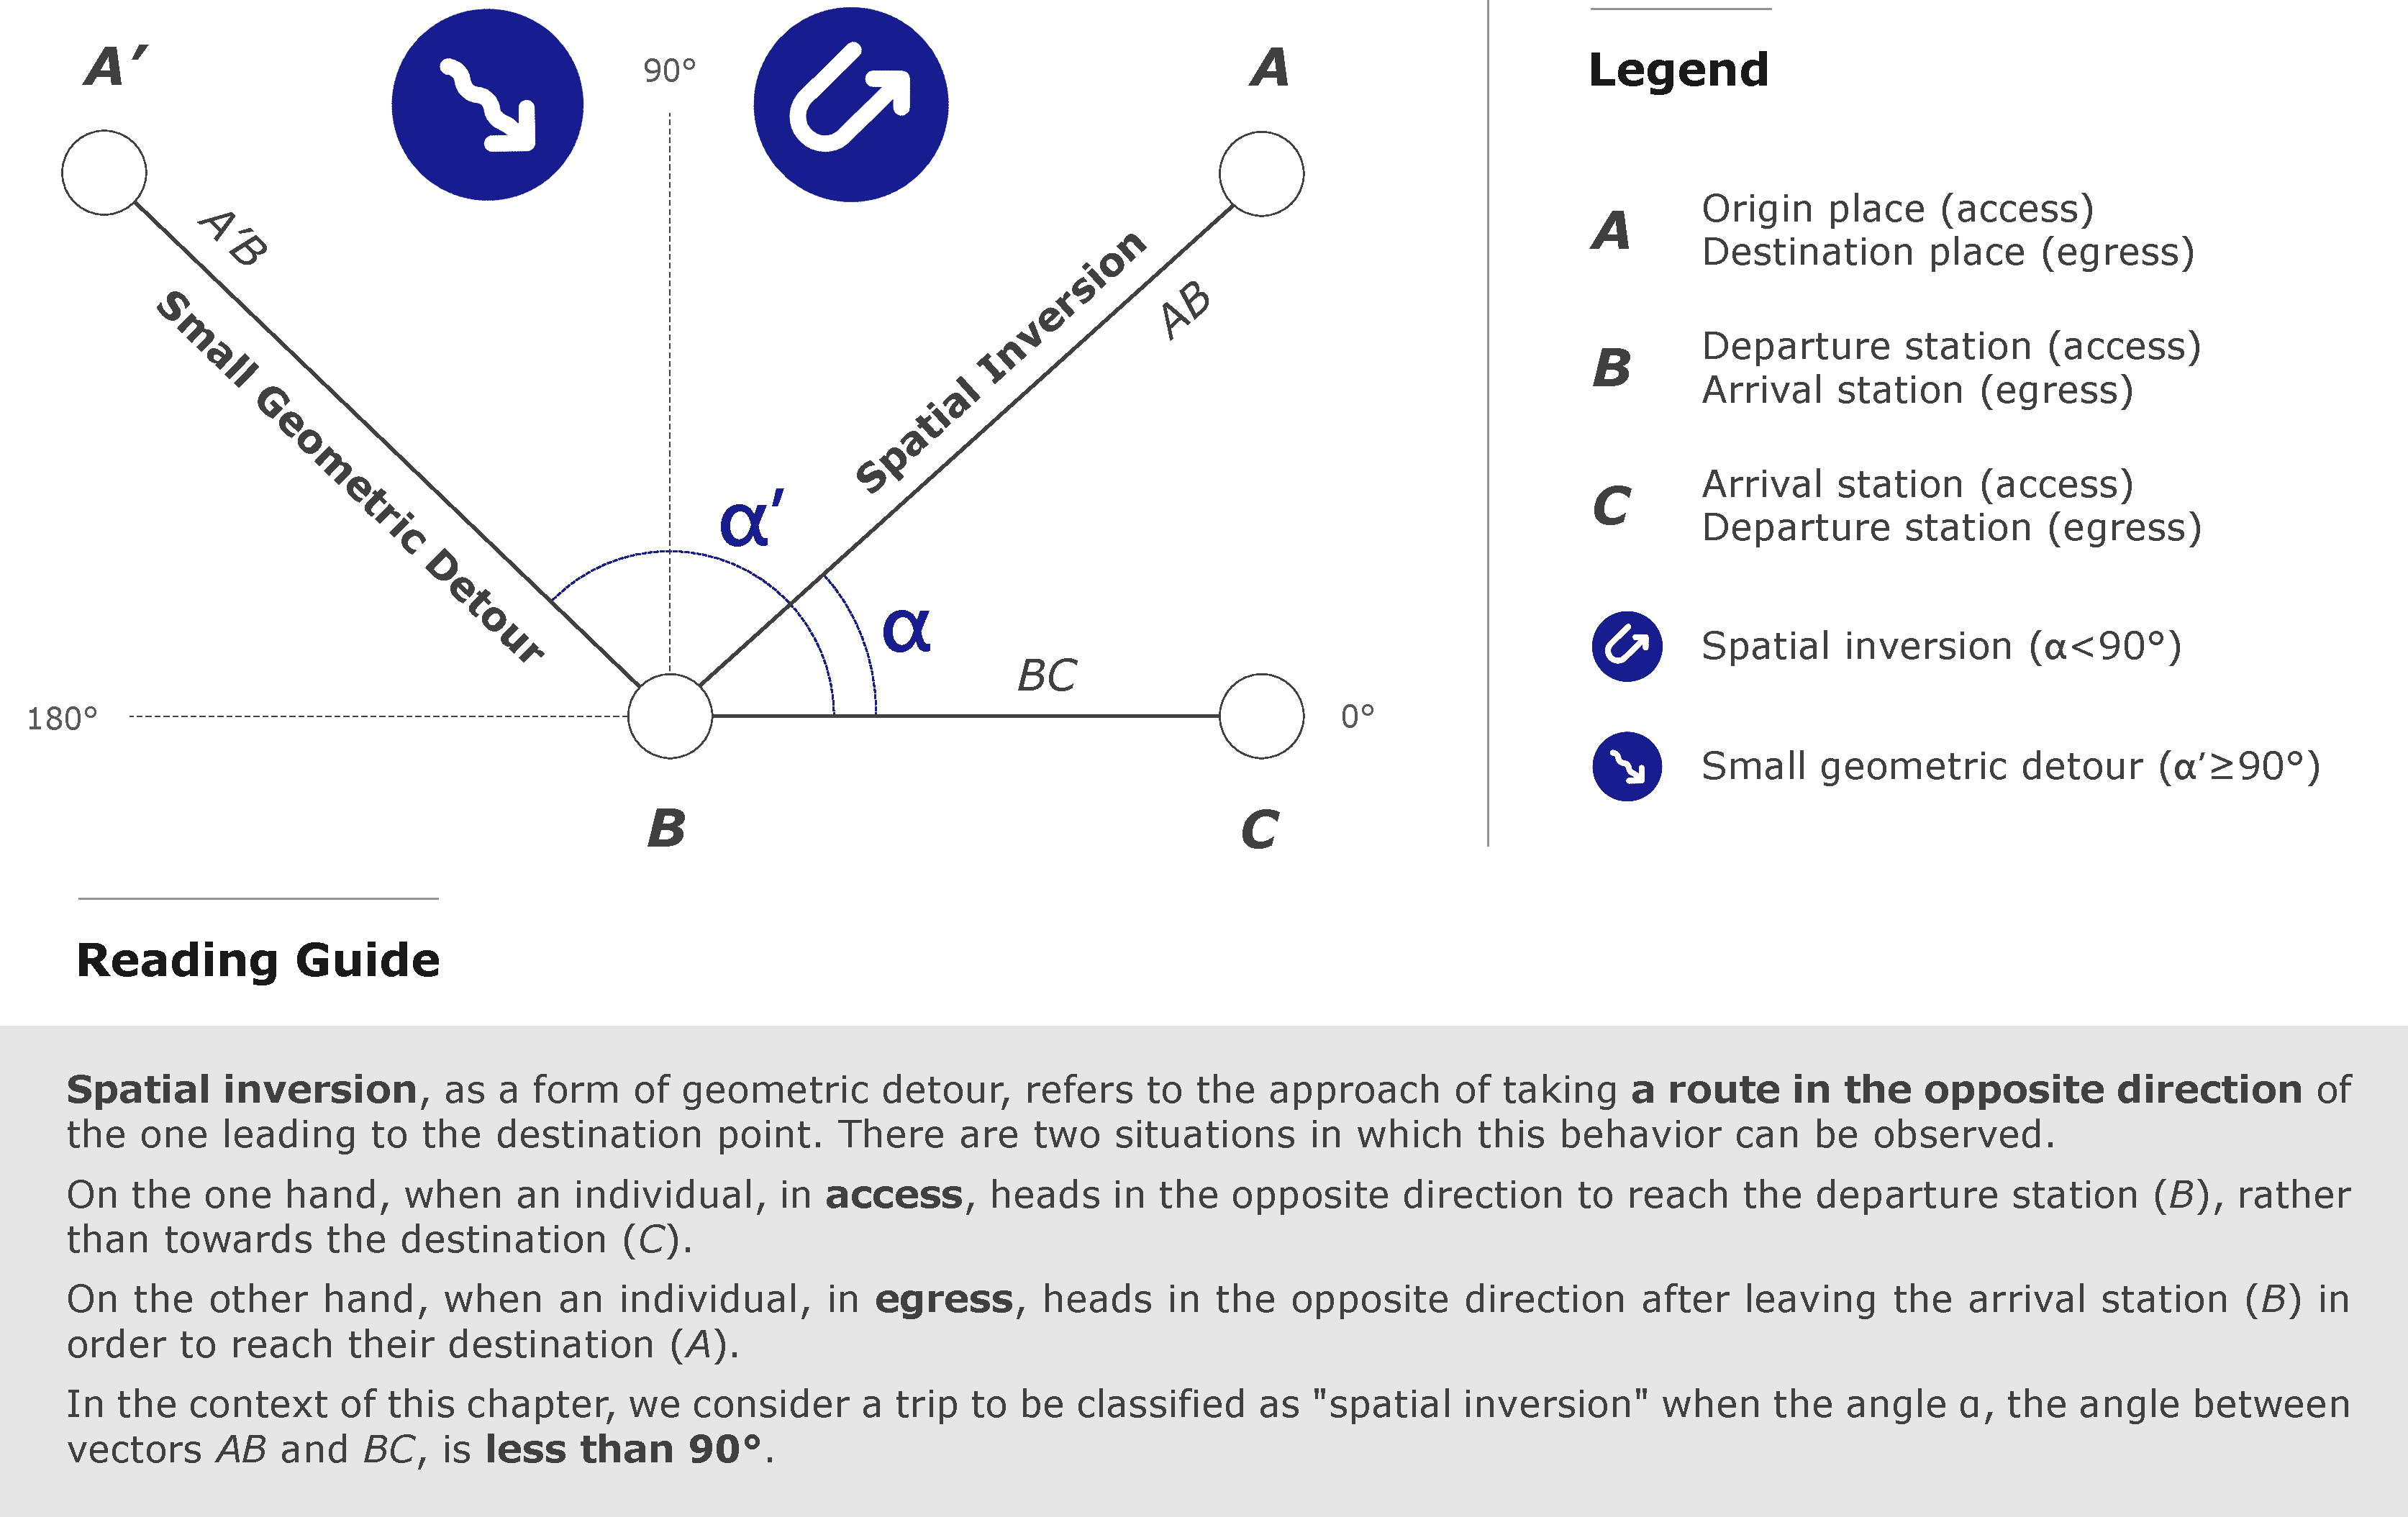
\includegraphics[width=1\columnwidth]{src/Figures/Chap-5/EN_Detours_Calcul_angles.pdf}}
    \vspace{5pt}
    \begin{flushright}\scriptsize{
    Author: \textcolor{blue}{Dylan Moinse (2023)}
    }\end{flushright}
\end{figure}

% Cartesian coordinates
After obtaining the geographic coordinates of points \(A\), \(B\), and \(C\), expressed in latitude and longitude using the \acrshort{WGS84} projection system\footnote{~
The \acrfull{WGS84} projection is a geographic coordinate system used to define the shape and position of the Earth. It is primarily used as the basis for satellite positioning systems such as \acrfull{GPS}.
}, we converted them into Cartesian coordinates (\(x\), \(y\), \(z\)) using the applicable conversion formulas for a sphere. Subsequently, by subtracting the Cartesian coordinates of points \(A\) and \(B\), then \(B\) and \(C\), we calculated the norms $\lVert \vec{AB} \rVert$ and $\lVert \vec{BC} \rVert$. These vectors were then used to determine their respective dot product ($\vec{AB} \cdot \vec{BC}$). Ultimately, we were able to deduce the angle between the vectors $\vec{AB}$ and $\vec{BC}$, expressed in radians and then in degrees ($\alpha$). The detailed calculations of the angles were provided in \hyperref[annexes:calcul-detours-angles]{Appendix~\ref{annexes:calcul-detours-angles}} (page~\pageref{annexes:calcul-detours-angles}).%%Translated%%

% Explanations
Once the angles $\alpha$ were measured, we generated an analysis grid in order to categorize the angles of the determined \acrshort{E-TVS} trips. By identifying extreme divergence shapes, such as spatial inversion, occurring when the angle $\alpha$ is between 0° and 90°, we are able to distinguish trips that involve significant geometric detours from straight-line paths.%%Translated%%

% 5.3.3.
\needspace{1\baselineskip} % Reserve space
\subsection{Characterization of Optimization Strategies
    \label{chap5:strategies-optimisation}
}

% Introduction
This section presents the results from the statistical analysis of trips involving detours and breaks. The first result will focus on the measured distances of \acrshort{E-TVS} trips, specifically identifying the distances traveled to make a detour. The determination of distance-time and spatial measures related to detours will then allow for the evaluation of the spatiotemporal optimization ratios of \acrshort{E-TVS} trips. Once the study has demonstrated the positive links between the presence of detours and the pursuit of movement optimization, it will proceed to classify the different types of optimization strategies through detours and breaks. Finally, the last result will present the categorization of users making intermodal detours, based on the determined optimization ratios.%%Translated%%

% 5.3.3.1.
\needspace{1\baselineskip} % Reserve space
\subsubsection*{An Extended Relevance Area of Light Individual Mobility around Stations
    \label{chap5:extension-accrue-quartier-gare}
}

% Analysis
Before considering the detours, it is essential to determine the distances traveled by bike and micromobility users, both for feeder and distribution trips, in order to assess the dimensions of the influence areas around public transport stations. Distance-time and spatial measures were calculated using the geographic coordinates collected through the questionnaire distributed as part of this doctoral research. To measure the socially acceptable detour distance performed by respondents, the 85\textsuperscript{th} percentile value was also used in the cumulative distribution applied \textcolor{blue}{\autocite[982]{lee_bicycle-based_2016}}\index{Lee, Jaeyeong|pagebf}\index{Choi, Keechoo|pagebf}\index{Leem, Yountaik|pagebf}.%%Translated%%

% Distances
Focusing on the sub-sample of 129 \acrshort{E-TVS} trips, and more specifically on the 171 bike or micromobility trips, both feeder and distribution, characterized by the presence of detours, the estimated distances for such trips are, unsurprisingly, higher. Across all types of light individual mobility, these \acrshort{E-TVS} trips have an acceptable spatial distance of 6.1 kilometers in the access stage and 5.2 kilometers in the egress stage, with respective medians of 2.7 and 2.3 kilometers. Among the various vehicles examined, the classic bike (78 trips) stands first, with a length of 6.7 kilometers and a median of 2.5 kilometers, followed by bike-sharing and shared micromobility (17 trips) with 4.4 and 2.9 kilometers, the folding bike (18 trips) with 6.5 and 2.4 kilometers, and the \acrshort{PeS} (36 trips) with 5.7 and 2.5 kilometers.%%Translated%%

% Detour distances
Compared to the estimated spatial distance of alternative trips (\(alt\)) made by bike or micromobility, \acrshort{E-TVS} trips (\(eff\)), particularly in the access stage, cover greater spatial distances. When comparing trips with and without detours, statistical analysis reveals a significant additional spatial distance for the former, of about two kilometers, or an additional travel time of ten minutes. Thus, users generate, on average, detours equivalent to two kilometers, representing nearly one-third of the total distance covered in the feeder and distribution stages by intermodal travelers using light individual mobility. This measure, related to the additional spatial distance carried by travelers, resonates with the empirical research of \textcolor{blue}{\textcite[11]{jin_competition_2019}}\index{Jin, Haitao|pagebf}\index{Jin, Fengjun|pagebf}\index{Wang, Jiao'e|pagebf}\index{Sun, Wei|pagebf}\index{Dong, Libo|pagebf}, which demonstrates that subway and bus users tend to replace short public transport connections of less than two kilometers with the use of \acrshort{DBS} in Beijing.%%Translated%%

% 5.3.3.2.
\needspace{1\baselineskip} % Reserve space
\subsubsection*{Detours as Catalysts for Distance Savings
    \label{chap5:detours-gains-de-temps}
}

% Detour rate
By cross-referencing the observed spatial distances (\(km_{eff}\)) with the spatial distances from alternative trips denoted (\(km_{alt}\)), we are able to determine the detour rate for the 129 \acrshort{E-TVS} commuting trips. The detour rate, as explained in the statistical analysis method, is an indicator where a value greater than 1 indicates that the actual route is longer than the shortest route. It appears that the average detour rate is 0.97 for all trips, with a median of 0.98 (see \hyperref[table-chap5:taux-detours]{Table~\ref{table-chap5:taux-detours}}, page~\pageref{table-chap5:taux-detours}). Statistically, this ratio has a standard deviation of 0.07, with a minimum value of 0.7 and a maximum value of 1.21. In general, \acrshort{E-TVS} trips made by bike or micromobility paradoxically seem to present relatively shorter spatial distances compared to alternative trips without detours. Moreover, the average ratio between the effective and alternative spatial distances is 5.75 for access routes (89 trips) and 7.73 for egress routes (81 trips). These substantial differences suggest that intermodal cyclists deliberately choose to make detours six to eight times longer on average in order to achieve spatial distance savings across their entire intermodal trip.%%Translated%%

    % Tableau Statistiques descriptives taux de détour E-TVS
% Descriptive statistics table for detour rates in E-TVS
%%Translated%%
    \begin{table}[h!]
    \centering
    \renewcommand{\arraystretch}{1.5}
    \resizebox{\columnwidth}{!}{
    \begin{tabular}{p{0.47\columnwidth}p{0.1\columnwidth}p{0.1\columnwidth}p{0.11\columnwidth}p{0.11\columnwidth}p{0.11\columnwidth}}
        %\hline
    \rule{0pt}{15pt} \textcolor{blue}{\textbf{Routes}} & \textcolor{blue}{\textbf{Rate}} & \textcolor{blue}{\textbf{$\sigma$}} & \textcolor{blue}{\textbf{Min.}} & \textcolor{blue}{\textbf{Max.}} & \textcolor{blue}{\textbf{Count}}\\
        \hline
    \multicolumn{6}{l}{\textbf{Overall journey}}\\
\small{Intermodal trip~($ km_{eff} $/$ km_{alt} $)} & \small{0.97} & \small{0.07} & \small{0.70} & \small{1.21} & \small{129}\\
        \hdashline
    \multicolumn{4}{l}{\textbf{Trip segments}}\\
\small{Access trip~($ km^{R}_{eff} $/$ km^{R}_{alt} $)} & \small{5.75} & \small{7.30} & \small{1.05} & \small{46.73} & \small{89}\\
\small{Egress trip~($ km^{D}_{eff} $/$ km^{D}_{alt} $)} & \small{7.73} & \small{14.23} & \small{1.09} & \small{115.22} & \small{81}\\
\small{Public transport trip~($ km^{TC}_{eff} $/$ km^{TC}_{alt} $)} & \small{0.90} & \small{0.12} & \small{0.45} & \small{1.15} & \small{129}\\
        \hline
        \end{tabular}}
    \caption{Detour rates for commuting journeys involving a detour.}
    \label{table-chap5:taux-detours}
        \vspace{5pt}
        \begin{flushleft}\scriptsize{
        \textcolor{blue}{Note:} $\sigma$ corresponds to the standard deviation.
        \\
        \textcolor{blue}{Reading Guide:} The detour rates for commuting journeys show that the last-mile and diffusion segments have very high detour rates, but these are compensated by an overall trip that is close to the optimal route.
        }\end{flushleft}
        \begin{flushright}\scriptsize{
        Author: \textcolor{blue}{Dylan Moinse (2023)}
        }\end{flushright}
        \end{table}%%Rédigé%%

% Circuit rate
The counterintuitive determination of the detour rate is supported by the measurement of the circuit rate coefficient, which takes into account the effective spatial distance of the \acrshort{E-TVS} trip (\(km_{eff}\)) and the spatial distance of the direct route without detour (\(km_{eud}\)). In this regard, the overall circuit rate of the \acrshort{E-TVS} trip reveals an additional spatial distance of 53\%, with an access circuit rate (89 trips) 8.34 times higher and an egress circuit rate (81 trips) 29.91 times higher. Furthermore, the statistical analysis of the circuit rate, based on the Euclidean distance, as well as the detour rate, based on the nearest public transport station, highlights an asymmetry between the first and last kilometers. Indeed, the trip leaving the station is characterized by much more pronounced detours than those observed when approaching it. More specifically, the egress circuit rate coefficient is 3.59 times higher, while the egress detour rate is 1.34 times greater.%%Translated%%

% Time detours
The positive relationship between detours and distance savings can also be reflected in an analysis examining the time-distance of \acrshort{E-TVS} trips. While the average total objective time (\(t_{O}\)) saved is 18.82\%, and the perceived time (\(t_{P}\)) is 17.56\%, illustrating the optimization process at play, \(t_{access}\) and \(t_{egress}\) are respectively 3.12 and 3.59 times longer than the shortest alternative trips. \textsl{A contrario}, \(t_{PT}\) and \(t_{waiting}\) are respectively 54.83\% and 79.58\% shorter due to these detours. Some authors have studied the circuit rate by bike and micromobility, in time distance, generally equal to 1.14 in Columbus, USA \textcolor{blue}{\autocite[195]{park_why_2019}}\index{Park, Yujin|pagebf}\index{Akar, Gulsah|pagebf}, and between 1.2 and 1.4 in Nanjing, China \textcolor{blue}{\autocite[10]{li_measuring_2022}}\index{Li, Xia|pagebf}\index{Liu, Zhenyu|pagebf}\index{Ma, Xinwei|pagebf}.%%Translated%%

    % Results modal substitution
Given the acceptable range of walking, which is reflected in certain estimated spatial distances, the legitimate question of modal substitution for walking arises. Although only 3 out of 129 \acrshort{E-TVS} trips have spatial distances of less than one kilometer—representing the average walking range to and from public transport stations according to our analysis—our observation concerns 25 alternative trips, which represent one fifth of the analyzed sample. Referring to one of the survey questions regarding modal substitution in the case of unavailability of the specific type of light individual mobility used, the 25 respondents who had the possibility of making trips of less than one kilometer for last-mile or distribution purposes report substituting walking and urban public transport with cycling or micromobility. Among this fifth of users, 17 out of the 25 individuals are men, averaging 33 years old, reflecting the total sample. However, this group of users substituting walking for light individual mobility is overrepresented by folding bicycles, whether electric or not, and underrepresented by classic bicycles and \acrshort{PeS}.%%Translated%%

    % Discussion modal substitution
According to the responses received, it is worth noting that 50 out of the 129 commuters surveyed, who made an \acrshort{E-TVS} trip, express a marked preference for using bicycles and micromobility over urban public transport. It should be emphasized that these individuals are mainly users of regional or high-speed rail services, and use these light modes of transport as a strategy to avoid the metro, tram, or bus. These mobility behaviors thus raise environmental questions, particularly regarding the development of \acrfull{e-Bike} and electric micromobility. Furthermore, these still under-researched mobility practices also hold potential, as they are capable of replacing short-distance trips made by urban public transport \textcolor{blue}{\autocite[328]{sun_can_2017}}\index{Sun, Guibo|pagebf}\index{Zacharias, John|pagebf}, potentially relieving congestion while ensuring savings related to the cost of tickets or subscriptions.%%Translated%%

    % Figure \Commas{modes rose}: Lyon map
    \begin{carte}[h!]\vspace*{4pt}
        \caption{The \Commas{\Marque{Rose des modes}}, a cartographic tool comparing intermodal travel times within the Lyon public transport network.}
        \label{fig-chap5:rose-modes-reseau-tcl}
        \centerline{\includegraphics[width=1\columnwidth]{src/Figures/Chap-5/EN_Detours_Rose_des_modes_TCL_FR.pdf}}
        \vspace{5pt}
        \begin{flushright}\scriptsize{
        Source: \textcolor{blue}{\textcite{tcl_transports_2023}}
        }\end{flushright}
    \end{carte}
    
    % Application TC + vélo + detours
The design of a synergy between light individual mobility and public transport networks, extending beyond the simple scale of the train station neighborhood to optimize intermodal travel, is reflected in several studies developed and applied by local authorities. In its Metropolitan Mobility Plan for 2035, \acrshort{MEL} advocates for an \Commas{\textsl{[extension of] the influence zone of stations and public transport stops through pedestrian-friendly infrastructure} [\dots] \textsl{to simplify the routes for certain public transport trips. Example: To take a bus at République coming from Lille Flandres station, one can walk 10 minutes.}}~\textcolor{blue}{\autocite[328]{conseil_de_developpement_de_la_mel_plan_2022}}\index{Conseil de développement de la MEL@\textsl{Conseil de développement de la MEL}|pagebf}. This approach, part of the urban strategy for the Lille metropolitan area, resonates with a report from the urban planning agency of \textsl{Bordeaux Aquitaine} \textcolor{blue}{\textcite{aurba_itineraires_2017}}\index{a'urba@\textsl{a'urba}|pagebf}, at the time under the direction of the French urban planner \textcolor{blue}{Jean-Marc Offner}\index{Offner, Jean-Marc|pagebf}, a leading expert on mobility and territorial planning issues. The document reestablishes the place of pedestrians in urban thinking, emphasizing that \Commas{\textsl{walking is not only useful near stations for public transport. Between stops, certain walking routes can efficiently complement the public transport network, helping to relieve congested central sections during peak hours}}~\textcolor{blue}{\autocite[3, 14, 24]{aurba_itineraires_2017}}\index{a'urba@\textsl{a'urba}|pagebf}. The report reveals the presence of many walking routes in Bordeaux, faster than the tram ride, over distances of up to fifteen or thirty minutes on foot. These routes, similar to mycorrhizae\footnote{~
Mycorrhiza is the result of a symbiosis between a fungus and a plant, two organisms with mutual benefits. Mycorrhizae form a dense network of filaments connected to plant roots, drawing nutrients from the soil that are inaccessible to the root system. In return, the plant provides the fungus with essential nutrients, such as carbohydrates, crucial for the fungus's survival. This biological symbiosis gives plants greater resilience, making them more adaptable to varied environmental conditions. By analogy, we could draw a parallel with the functional complementarity between light individual mobility and the public transport system, as this relationship enhances the resilience of the mobility system while contributing to a more \gls{sustainable} urban ecosystem.
} offer a significant reduction in travel time, at least one third shorter compared to a journey solely by tram. This study enabled the Bordeaux urban planning agency to identify and diagnose strategic \Commas{pedestrian crossings} that should benefit from improved \gls{walkability}.%%Translated%%

    % Figure \Commas{modes rose}: Part Dieu example
    \begin{carte}[h!]\vspace*{4pt}
        \caption{The \Commas{\Marque{Rose des modes}} applied to the Part Dieu station, in Lyon.}
        \label{fig-chap5:rose-modes-reseau-part-dieu}
        \centerline{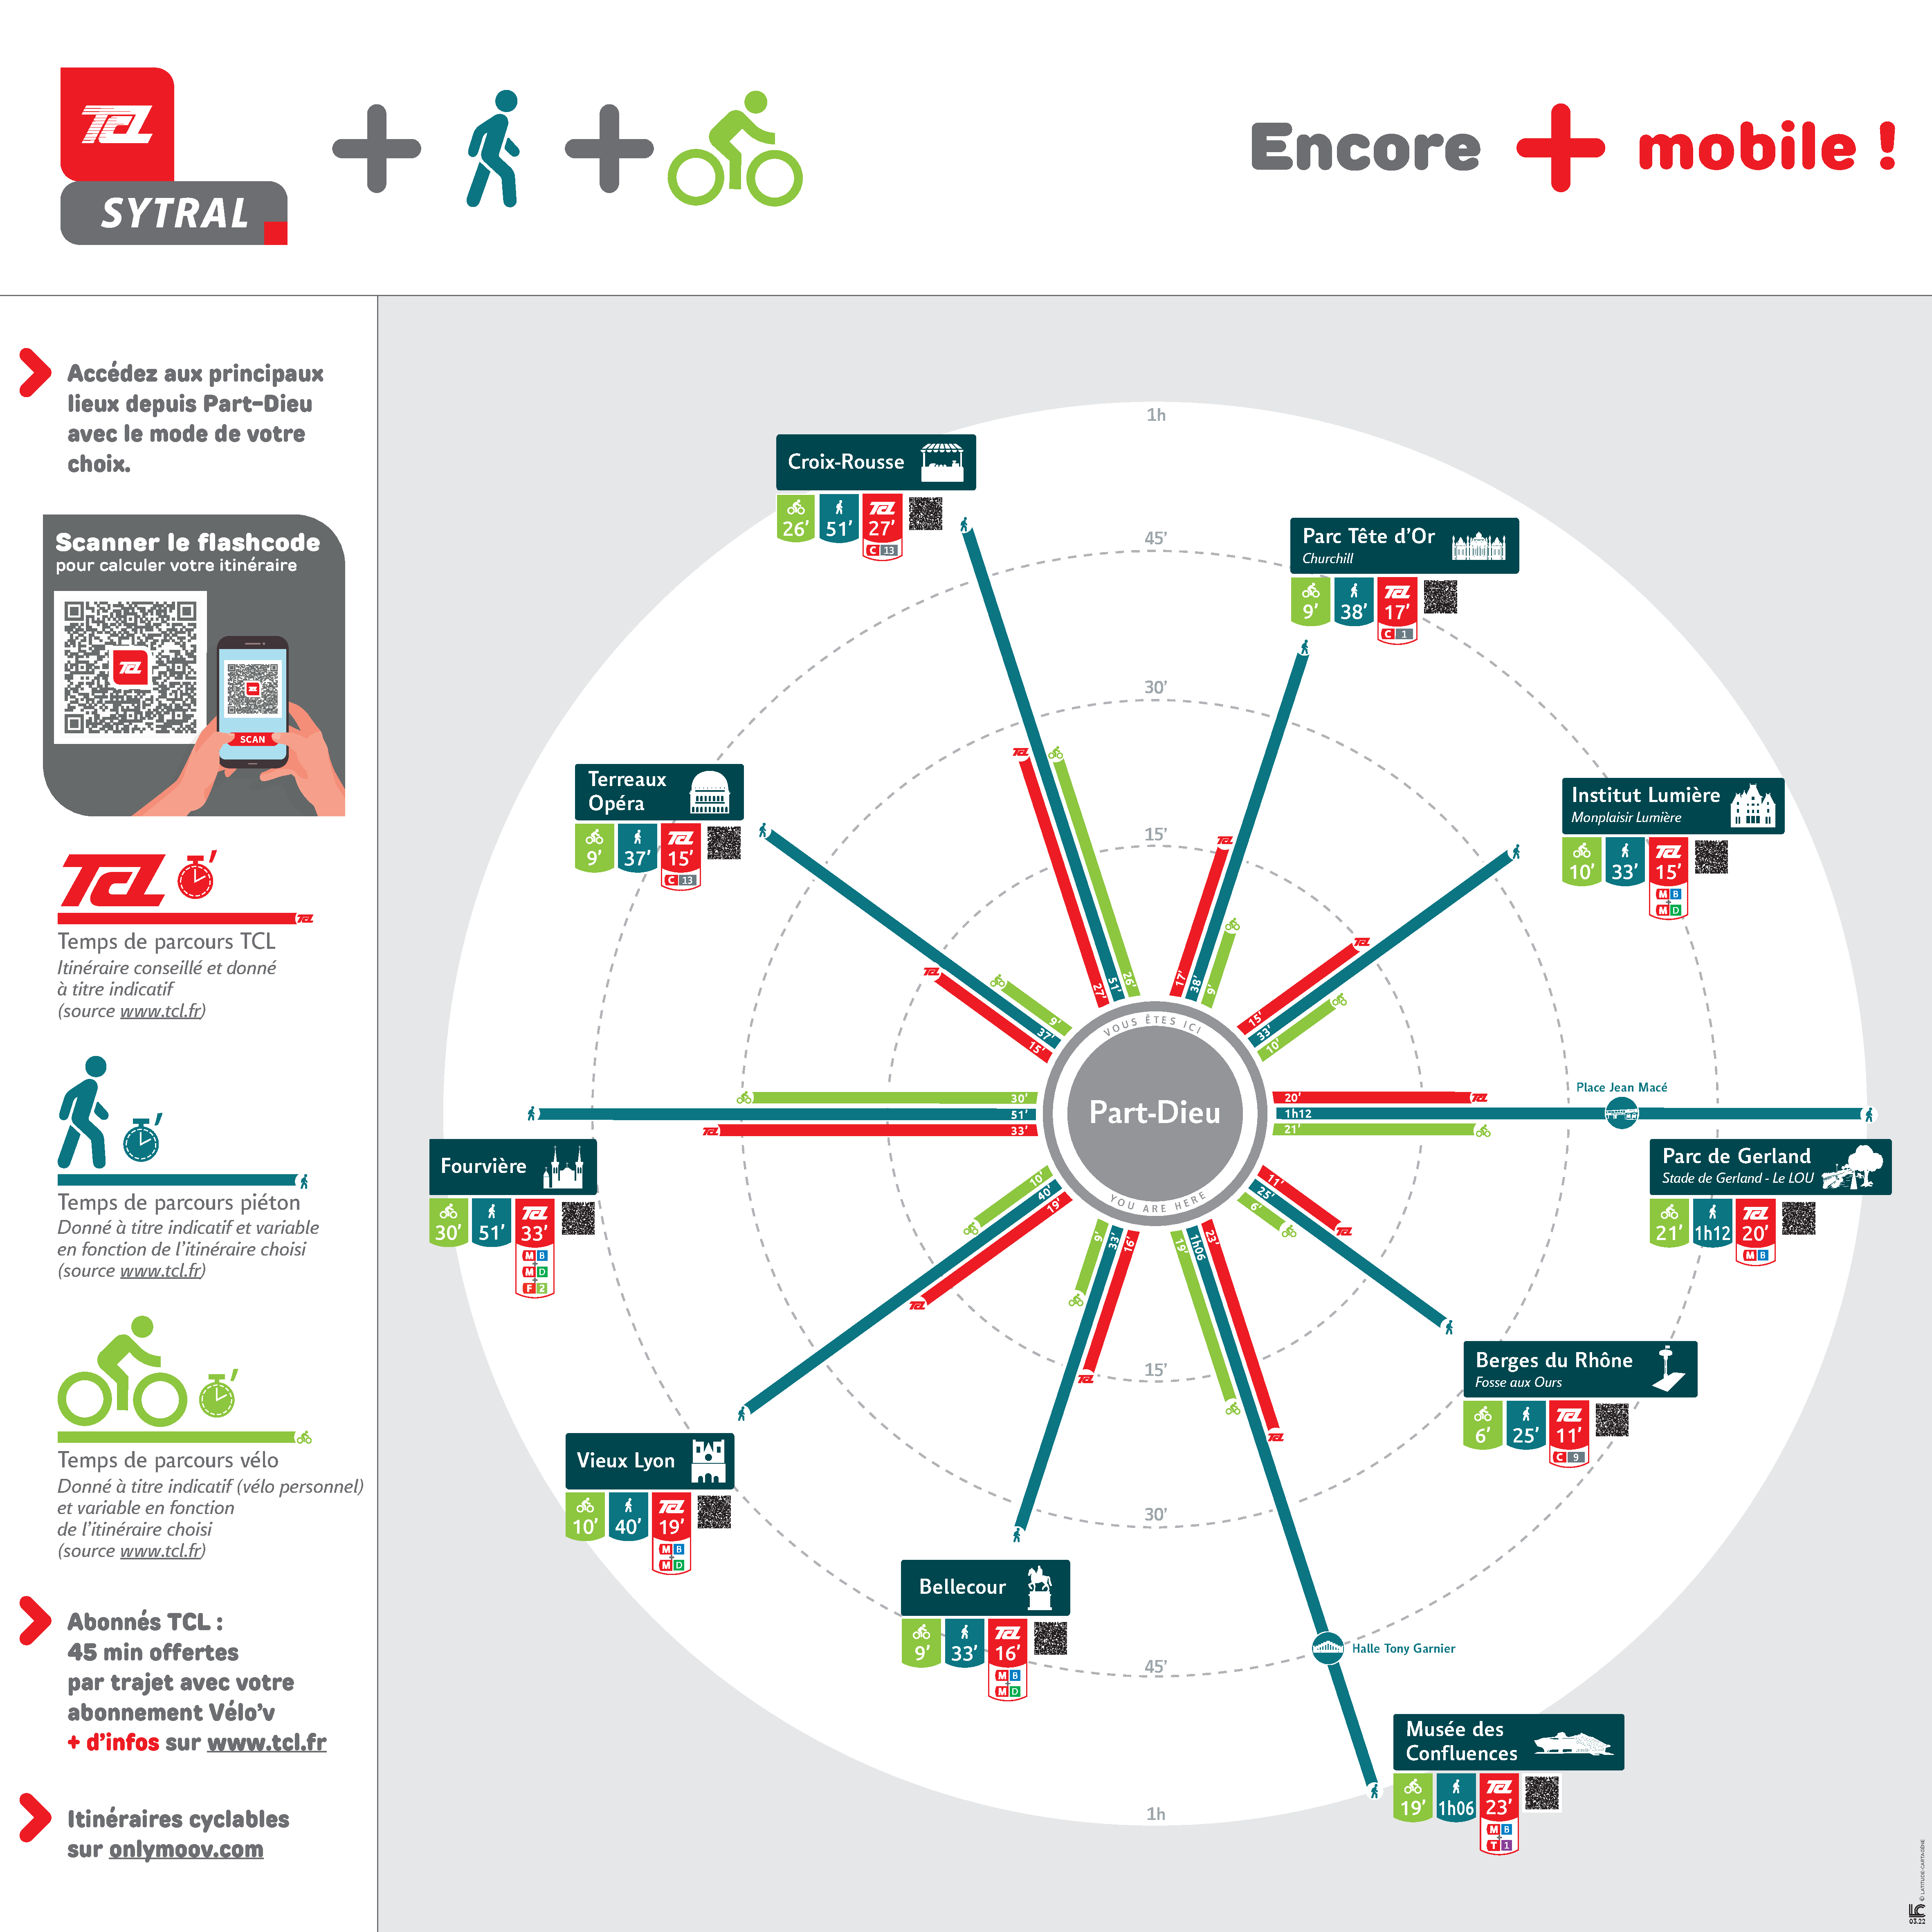
\includegraphics[width=1\columnwidth]{src/Figures/Chap-5/EN_Detours_Part_Dieu_rose_des_modes_TCL_FR.pdf}}
        \vspace{5pt}
        \begin{flushright}\scriptsize{
        Source: \textcolor{blue}{\textcite{tcl_transports_2023}}
        }\end{flushright}
    \end{carte}

    In the context of optimizing and efficiently alleviating congestion in the public transport network, \acrshort{MEL} and \textsl{Bordeaux Métropole} are implementing an innovative strategy by revaluing the role of combined walking. This initiative is part of a broader context of rethinking urban mobility practices, where walking, often relegated to a secondary role, is now recognized as a central and complementary element of public transport systems. At the same time, the question of the role of light individual mobility in these reflections also arises. In this regard, the strategy implemented by \textsl{Métropole de Lyon} is particularly interesting with respect to the optimization potential of bicycles integrated into public transport. The initiative led by the Lyon metropolitan area relies on the development of a tool called the \Marque{Rose des modes}, created by the mapping agency \Marque{Latitude-Cartagène}. This visual representation aims to provide information on travel times to various destinations from a given point, integrating the public transport network in Lyon, walking, and cycling \textcolor{blue}{\autocite{latitude-cartagene_rose_nodate}}\index{Latitude-Cartagène@\textsl{Latitude-Cartagène}|pagebf}, as shown in \hyperref[fig-chap5:rose-modes-reseau-tcl]{Map~\ref{fig-chap5:rose-modes-reseau-tcl}} (page~\pageref{fig-chap5:rose-modes-reseau-tcl}). This \gls{cartography} serves as an informational tool for travelers and facilitates intermodality. In October 2021, \textcolor{blue}{\textcite[15]{keolis_lyon_rapport_2022}}\index{Keolis@\textsl{Keolis}|pagebf} experimented with this signage in two metro stations, before expanding the project to ten metro stations and eight tram stops, highlighting reduced travel times, limited transfers, and alternatives in case of network disruptions \textcolor{blue}{\autocite[15]{keolis_lyon_rapport_2022}}\index{Keolis@\textsl{Keolis}|pagebf}. The example around the Part Dieu station shows that, for seven of the ten selected iconic destinations, the bicycle route, shown in green, is theoretically faster than urban public transport from the station, indicated in red (see \hyperref[fig-chap5:rose-modes-reseau-part-dieu]{Map~\ref{fig-chap5:rose-modes-reseau-part-dieu}}, page~\pageref{fig-chap5:rose-modes-reseau-part-dieu}). The introduction of the \Commas{\Marque{Rose des modes}} is among the six winners of the 2022 edition of the \textsl{Talents de la marche} competition, in the transport operators category \textcolor{blue}{\autocite{club_des_villes_et_territoires_cyclables_six_nodate}}\index{Club des villes et territoires cyclables et marchables@\textsl{Club des villes et territoires cyclables et marchables}|pagebf}.%%Translated%%

    % Nudges
These various initiatives implemented by local authorities are part of the behavioral design strategy known as \Commas{\textsl{nudge}}. This concept, popularized by behavioral economics theorist \textcolor{blue}{Richard Thaler} in his book \foreignlanguage{english}{\textsl{Nudge: Improving Decisions About Health, Wealth, and Happiness}}\footnote{~
    \Commas{Nudge: \textsl{Améliorer les décisions concernant la santé, la richesse et le bonheur}}. Note that \textsl{nudge} can be translated into French as \Commas{coup de pouce}.
    } \textcolor{blue}{\autocite{thaler_nudge_2009}}\index{Thaler, Richard~H.|pagebf}\index{Sunstein, Cass~R.|pagebf}, is based on subtle and light interventions that make a choice more attractive and easier for users to adopt. According to \textcolor{blue}{\textcite[12]{lehner_nudging_2016}}\index{Lehner, Matthias|pagebf}\index{Mont, Oksana|pagebf}\index{Heiskanen, Eva|pagebf}, a \textsl{nudge}, designed on the basis of cognitive and social psychology and behavioral economics, is defined as \Commas{\textsl{instruments [that] rely mainly on the idea of choice architecture, which may include changes in infrastructure or the environment that guide and enable individuals to make choices almost automatically, where information provided is simplified or where default options are offered in a way that improves people's well-being. Thus, nudges do not aim to change someone's value system or increase the provision of information; they focus rather on facilitating behaviors and private decisions that are beneficial to individuals and often also to society.}}\footnote{~
    \Commas{\textsl{The instruments [\textsl{nudges}] rely heavily on the idea of choice architecture that may include changes in infrastructure or the environment that guide and enable individuals to make choices almost automatically, where information provided is simplified or where defaults are offered in a way that makes people better off. Thus, nudges do not try to change one’s value system or increase information provision; instead they focus on enabling behaviours and private decisions that are good for the individuals and often for the society as well.}}~\textcolor{blue}{\autocite[12]{lehner_nudging_2016}}\index{Lehner, Matthias|pagebf}\index{Mont, Oksana|pagebf}\index{Heiskanen, Eva|pagebf}.
} [free translation]. One of the four key components of \textsl{nudging}\footnote{~
    \textsl{Nudging} encompasses four types of policy instruments according to \textcolor{blue}{\textcite[22]{lehner_nudging_2016}}\index{Lehner, Matthias|pagebf}\index{Mont, Oksana|pagebf}\index{Heiskanen, Eva|pagebf}: (i) simplification and framing of information, (ii) changes in the physical environment, (iii) changes in default policies, and (iv) use of social norms.
} lies in the simplification and framing of information, aiming to make the information more accessible and tailored to its audience \textcolor{blue}{\autocite[22]{lehner_nudging_2016}}\index{Lehner, Matthias|pagebf}\index{Mont, Oksana|pagebf}\index{Heiskanen, Eva|pagebf}. Furthermore, to be qualified as a true \textsl{nudge}, three conditions must be met: (i) the manipulation must concern the means, not the ends, (ii) freedom of choice must be preserved in the alternatives presented, and (iii) the reward or cost must be light (\Commas{\textsl{soft}}), implying decisions with low involvement or passive habitual behavior \textcolor{blue}{\autocite[199]{rachlin_choice_2015}}\index{Rachlin, Howard|pagebf}. In the context of mobility, the \textsl{nudge} is introduced as a method seeking to guide the modal choice decision-making process in the desired direction. Changing the mental, social, and physical environment, or presenting choices differently, can increase the likelihood that an alternative becomes the preferred option \textcolor{blue}{\autocite[12]{mont_nudging_2014}}\index{Mont, Oksana|pagebf}\index{Lehner, Matthias|pagebf}\index{Heiskanen, Eva|pagebf}, much like the \Commas{\Marque{Rose des modes}}.%%Translated%%

% 5.3.3.3.
\needspace{1\baselineskip} % Reserve space
\subsubsection*{Spatial Inversion, the Driver of Spatiotemporal Optimization
    \label{chap5:inversion-spatiale-optimisation}
    }
 
% Introduction
Based on the angles $\alpha$ measured for each route involving a detour (see the \hyperref[chap5:calcul-angles-detours]{subsection related to the calculation of angles}, page~\pageref{chap5:calcul-angles-detours}), it was possible to understand the extent to which following a route in the opposite direction to the destination actually leads to space and time savings. To this end, we considered both the folding and egress angles $\alpha$. A simplified analytical framework was applied to characterize the measured angles: spatial inversion occurs when the angle $\alpha$ between the vectors $\vec{AB}$ and $\vec{BC}$ is less than 90°, indicating a direction relatively opposite to the destination.%%Translated%%

   % Difference between eff and alt angles
By comparing the angles obtained from the \acrshort{E-TVS} routes ($\alpha_{eff}$) with those from the shortest routes ($\alpha_{alt}$), it appears that routes involving detours exhibit a less direct geometric shape toward the destination. Thus, the \(eff\) routes have an average angle of 76.70°, indicating a slight spatial inversion, in contrast to the \(alt\) routes, whose average angle is 110.50°. However, this statistical analysis reveals significant disparities between routes that involve folding toward a public transport station and those that involve egress from a station. The spatial inversion of $\alpha_{eff}$ is more pronounced in the first kilometers (70.74°) than in the last kilometers (83.29°) of public transport. Nevertheless, comparing them with $\alpha_{alt}$ highlights a greater tendency for spatial inversion in egress rather than in access. While the difference between $\alpha_{eff}$ and $\alpha_{alt}$ is only 22.18\% for the access route, this tendency to change direction rises to 64.51\% for the exit route from the public transport station.%%Translated%%
 
% Correlation between spatial inversion and time saved
In this regard, \hyperref[fig-chap5:regression-detour-gain-temps]{Figure~\ref{fig-chap5:regression-detour-gain-temps}} (page~\pageref{fig-chap5:regression-detour-gain-temps}) highlights a positive association between the geometric configuration of detours, taking the form of spatial inversion, and the estimated objective time savings through the temporal optimization ratio (\(R_{t{(O)}}\)). It appears that, all other factors being equal, an \acrshort{E-TVS} route with a spatial inversion geometrically tends to generate substantial time savings compared to an \acrshort{E-TVS} route where the detour's geometric shape is more direct.%%Translated%%

% Figure correlation between angles and time ratio
    \begin{figure}[h!]\vspace*{4pt}
        \caption{Linear regression between the detour shape of the route and the objective time savings.}
        \label{fig-chap5:regression-detour-gain-temps}
        \centerline{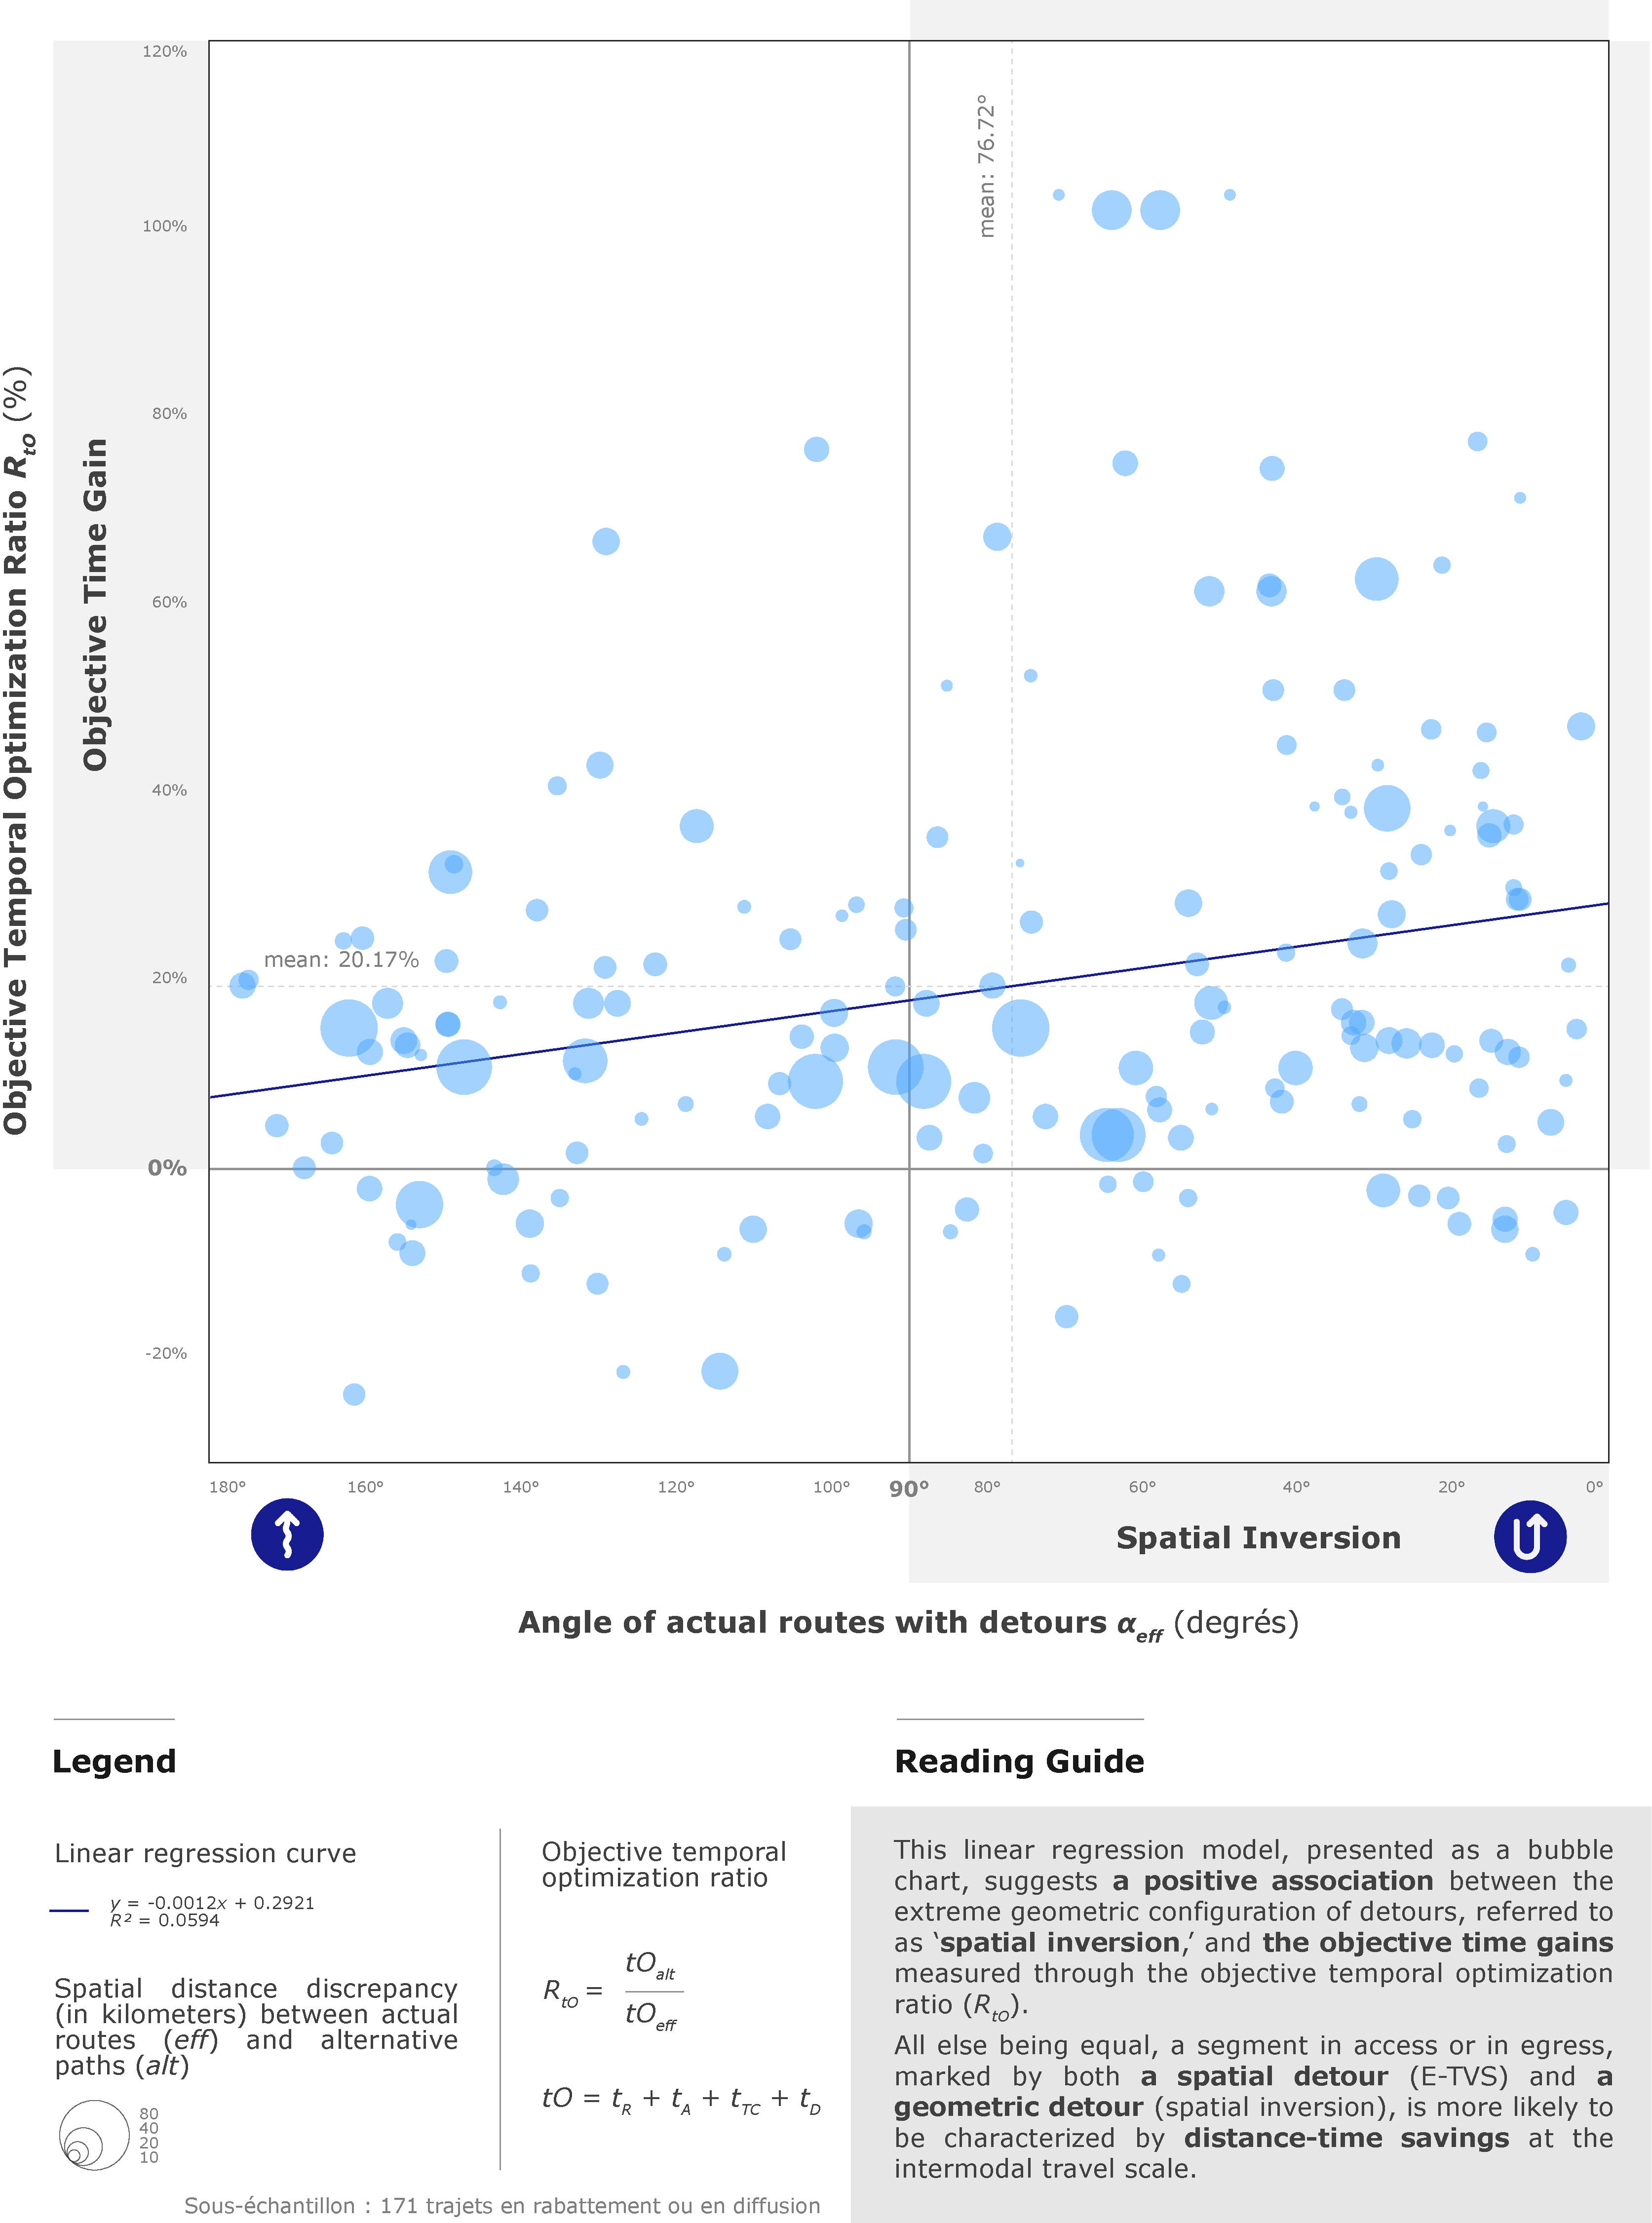
\includegraphics[width=1\columnwidth]{src/Figures/Chap-5/EN_Detours_Ratios_angles.pdf}}
        \vspace{5pt}
        \begin{flushright}\scriptsize{
        Author: \textcolor{blue}{Dylan Moinse (2023)}
        %\\
        %Created with \Marque{Python}~and \Marque{Illustrator}
        }\end{flushright}
    \end{figure}

% Egress
In this context, the statistical results suggest a higher tendency among users to opt for larger detours during their egress journeys. This distinction between folding and egress routes could be partly explained by variations in individual \gls{perception} of time between the different phases of an intermodal trip. In this regard, the study published by \textcolor{blue}{\textcite[79]{schakenbos_valuation_2016}}\index{Schakenbos, Rik|pagebf}\index{La Paix Puello, Lissy|pagebf}\index{Nijënstein, Sandra|pagebf}\index{Geurs, Karst~T.|pagebf} highlights a different relationship to the cost associated with bus transfers between the folding route, lasting about thirteen minutes, and the egress route, reduced to six minutes. Meanwhile, \textcolor{blue}{\textcite[3]{romm_differences_2022}}\index{Romm, Daniel|pagebf}\index{Verma, Priyanka|pagebf}\index{Karpinski, Elizabeth|pagebf}\index{Sanders, Tracy~L.|pagebf}\index{McKenzie, Grant|pagebf} demonstrated that stations near the termini of metro lines in Boston show higher potential bike-sharing activity for the segment related to the last kilometers, while stations in the urban center exhibit more activity for the first kilometers.%%Translated%%

% Commented routes
The question of spatial inversion appears to play a crucial role in the modal choices made by travelers. Through a commented journey conducted on \acrshort{PeS} and \acrshort{TER}, exchanges with participant \(PCTE_{1}\) referring to spatial inversion can be cited. This participant expressed a strong preference for using the electric scooter to reach Lille Flandres station, despite the presence of a metro line crossing her neighborhood and directly serving the station in only two stops. The first reason cited by this user concerns the fear of disruptions in the urban public transport network, which could force her to miss her \acrshort{TER}, which has a low frequency. However, a geographical factor adds to this consideration. Indeed, the location of the nearest metro station to her home, the Saint-Maurice Pellevoisin stop (line 2 of the \textsl{Ilévia} network), is, in her words, \Commas{in the opposite direction of the station} [12:18, \(PCTE^{TC}_{1}\)], as illustrated by \hyperref[fig-chap5:pcte1a-inversion-spatiale]{Figure~\ref{fig-chap5:pcte1a-inversion-spatiale}} (page~\pageref{fig-chap5:pcte1a-inversion-spatiale}). The participant thus expresses a sense of time lost due to the geometric shape of the route to access the metro line. \Commas{It's silly, but I feel like I'm wasting time turning around to go to the metro\dots} [12:18, \(PCTE^{TC}_{1}\)], she confides. It is interesting to note that this reflection related to the modal choice of the scooter over the metro concerns only the access journey, from her home to her workplace. The participant seems less aware of such spatial inversion during her egress journey from Maubeuge station. This observation highlights a tendency to favor individual mobility for more direct routes to public transport stations, particularly when reaching them, in order to benefit from more direct routes. Users are thus led to take detours, either to obtain more direct geometric paths or, conversely, to access more efficient public transport systems by following spatial inversion.%%Translated%%

%% Figure 1 Commented route PCTE1A
    \begin{figure}[h!]\vspace*{4pt}
        \caption{Image extracted from the filmed route on the folding path towards Lille Flandres station, illustrating a spatial inversion situation (\(PCTE^{A}_{1}\)).}
        \label{fig-chap5:pcte1a-inversion-spatiale}
        \centerline{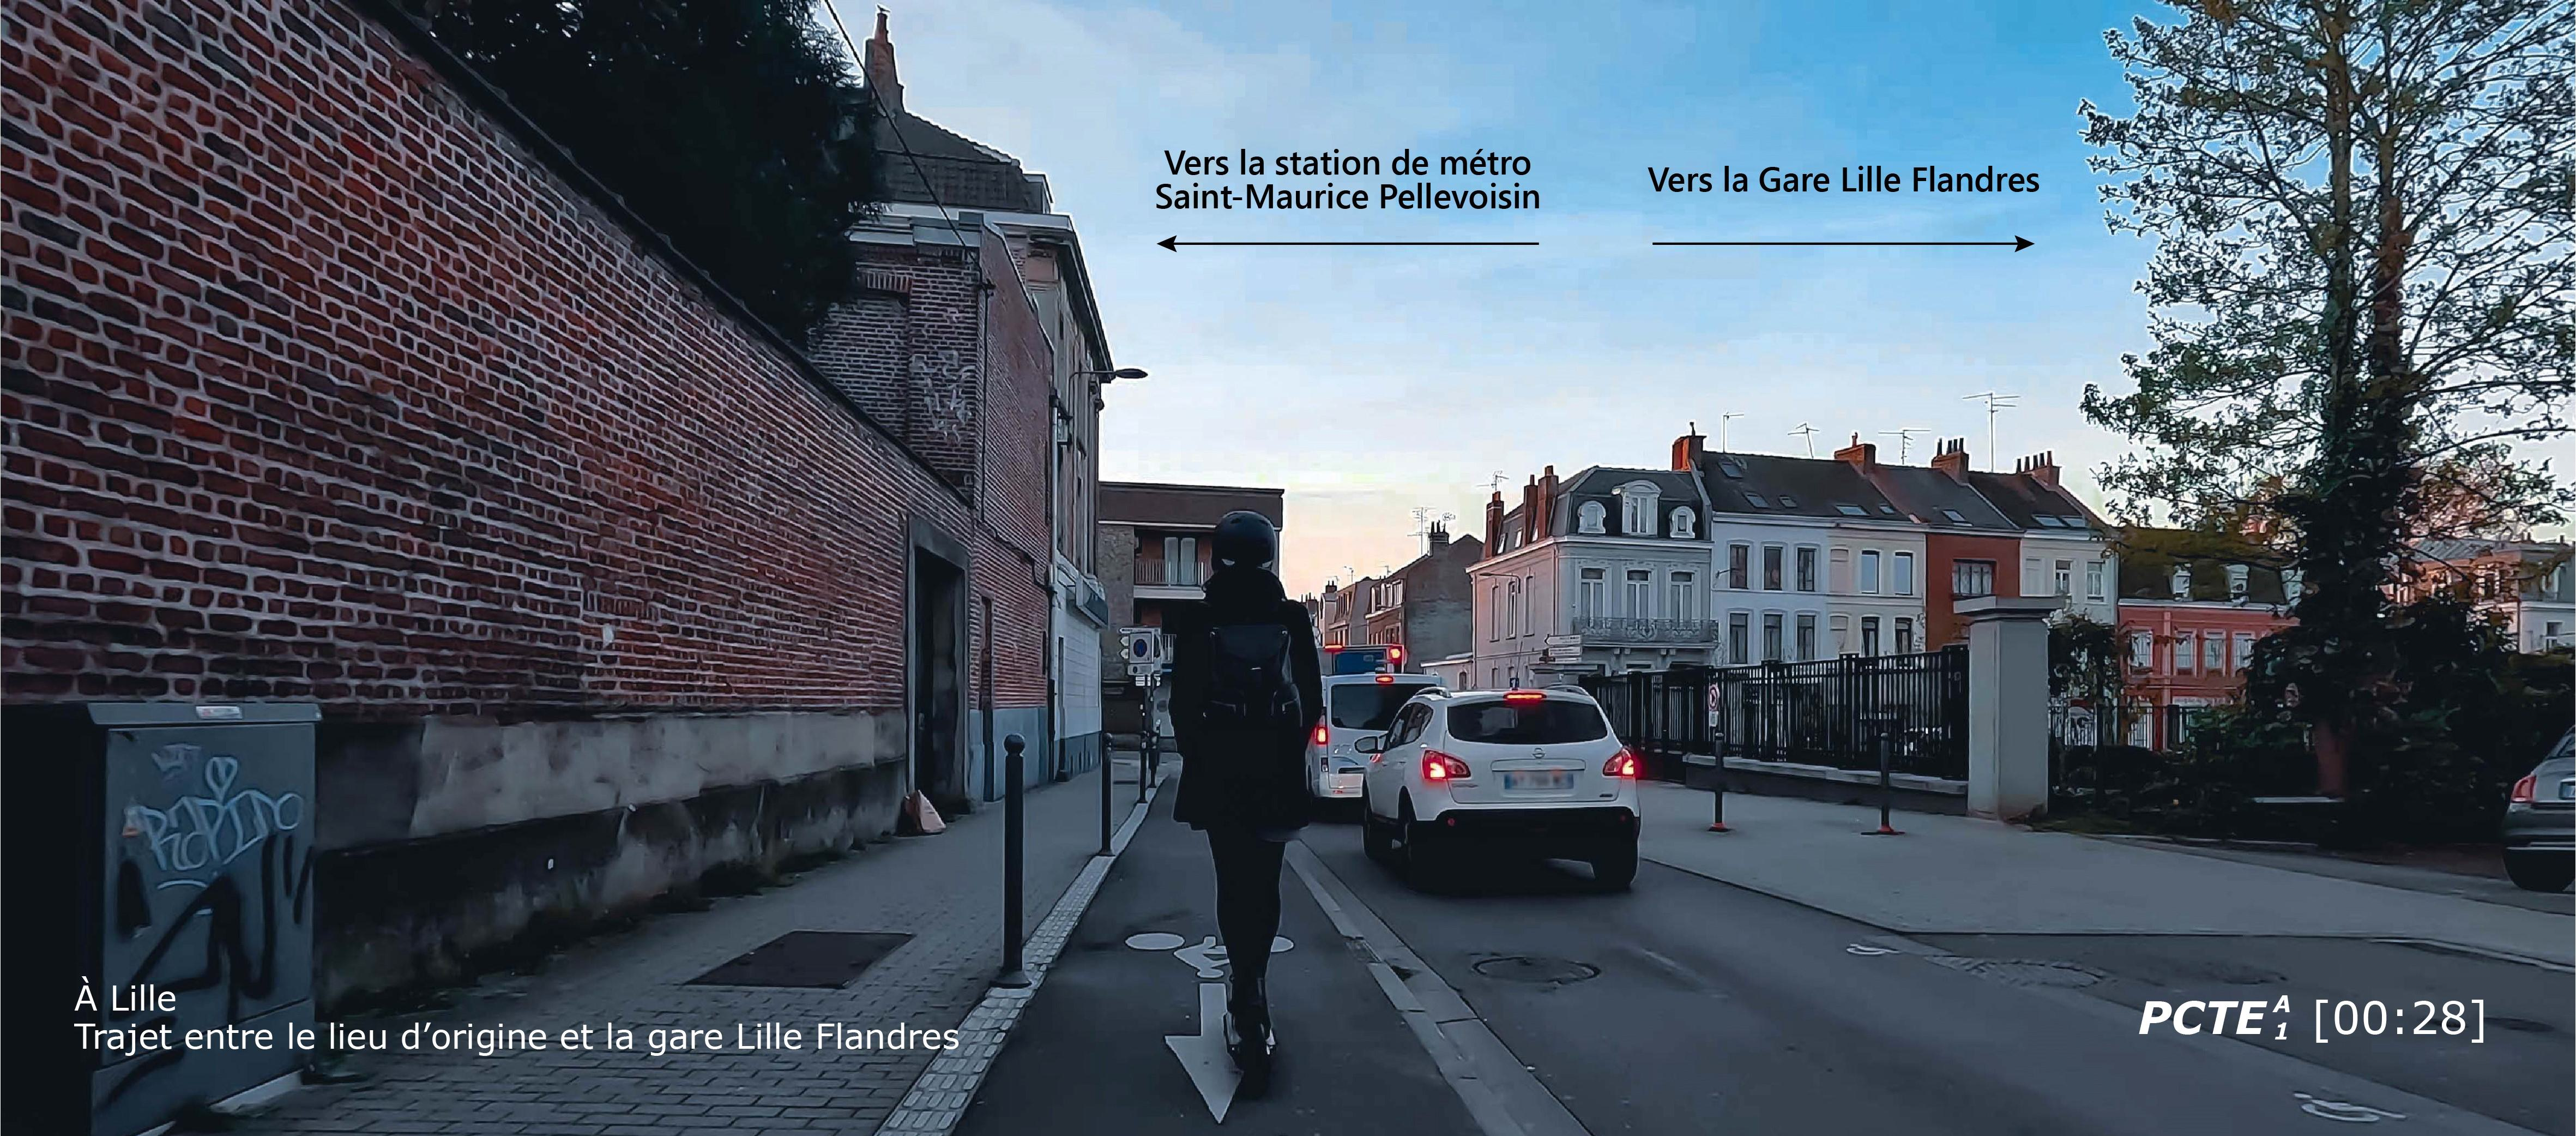
\includegraphics[width=1\columnwidth]{src/Figures/Chap-5/EN_Detours_PCTE1_Access_1.jpg}}
        \vspace{5pt}
        \begin{flushright}\scriptsize{
        Author: \textcolor{blue}{Dylan Moinse (2022)}
        }\end{flushright}
    \end{figure}

% 5.3.3.4.
\needspace{1\baselineskip} % Reserve space
\subsubsection*{Typology of Optimization Strategies Based on Detours and Breaks
    \label{chap5:typologie-strategies-optimisation}
    }
 
% Classification of detours
The statistical analysis of the surveyed commuters was complemented by a geostatistical analysis of the \acrshort{E-TVS} routes, which allowed us to identify different categories of optimization strategies primarily based on detours. We developed a classification of the three main types of detours identified, depending on the context in which the spatiotemporal optimization of movement is sought, in accordance with \hyperref[fig-chap5:classification-strategies-optimisation-detours]{Map~\ref{fig-chap5:classification-strategies-optimisation-detours}} (page~\pageref{fig-chap5:classification-strategies-optimisation-detours}). The first type of mobility behavior is referred to as (i) \Commas{avoidance of transfers,} the second (ii) \Commas{more attractive public transport station,} and the last (iii) \Commas{reduction of time spent on public transport.}%%Translated%%

% Methodology
The analytical approach chosen to classify intermodal routes involving detours was based on the evaluation of several critical dimensions: (i) the spatial and temporal distances traveled, (ii) the total number of transfers required, (iii) the frequency of service provided by the public transport network, and (iv) the waiting time at the station. %%Translated%%

%% Figure correlation between angles and time ratio
    \begin{carte}[h!]\vspace*{4pt}
        \centerline{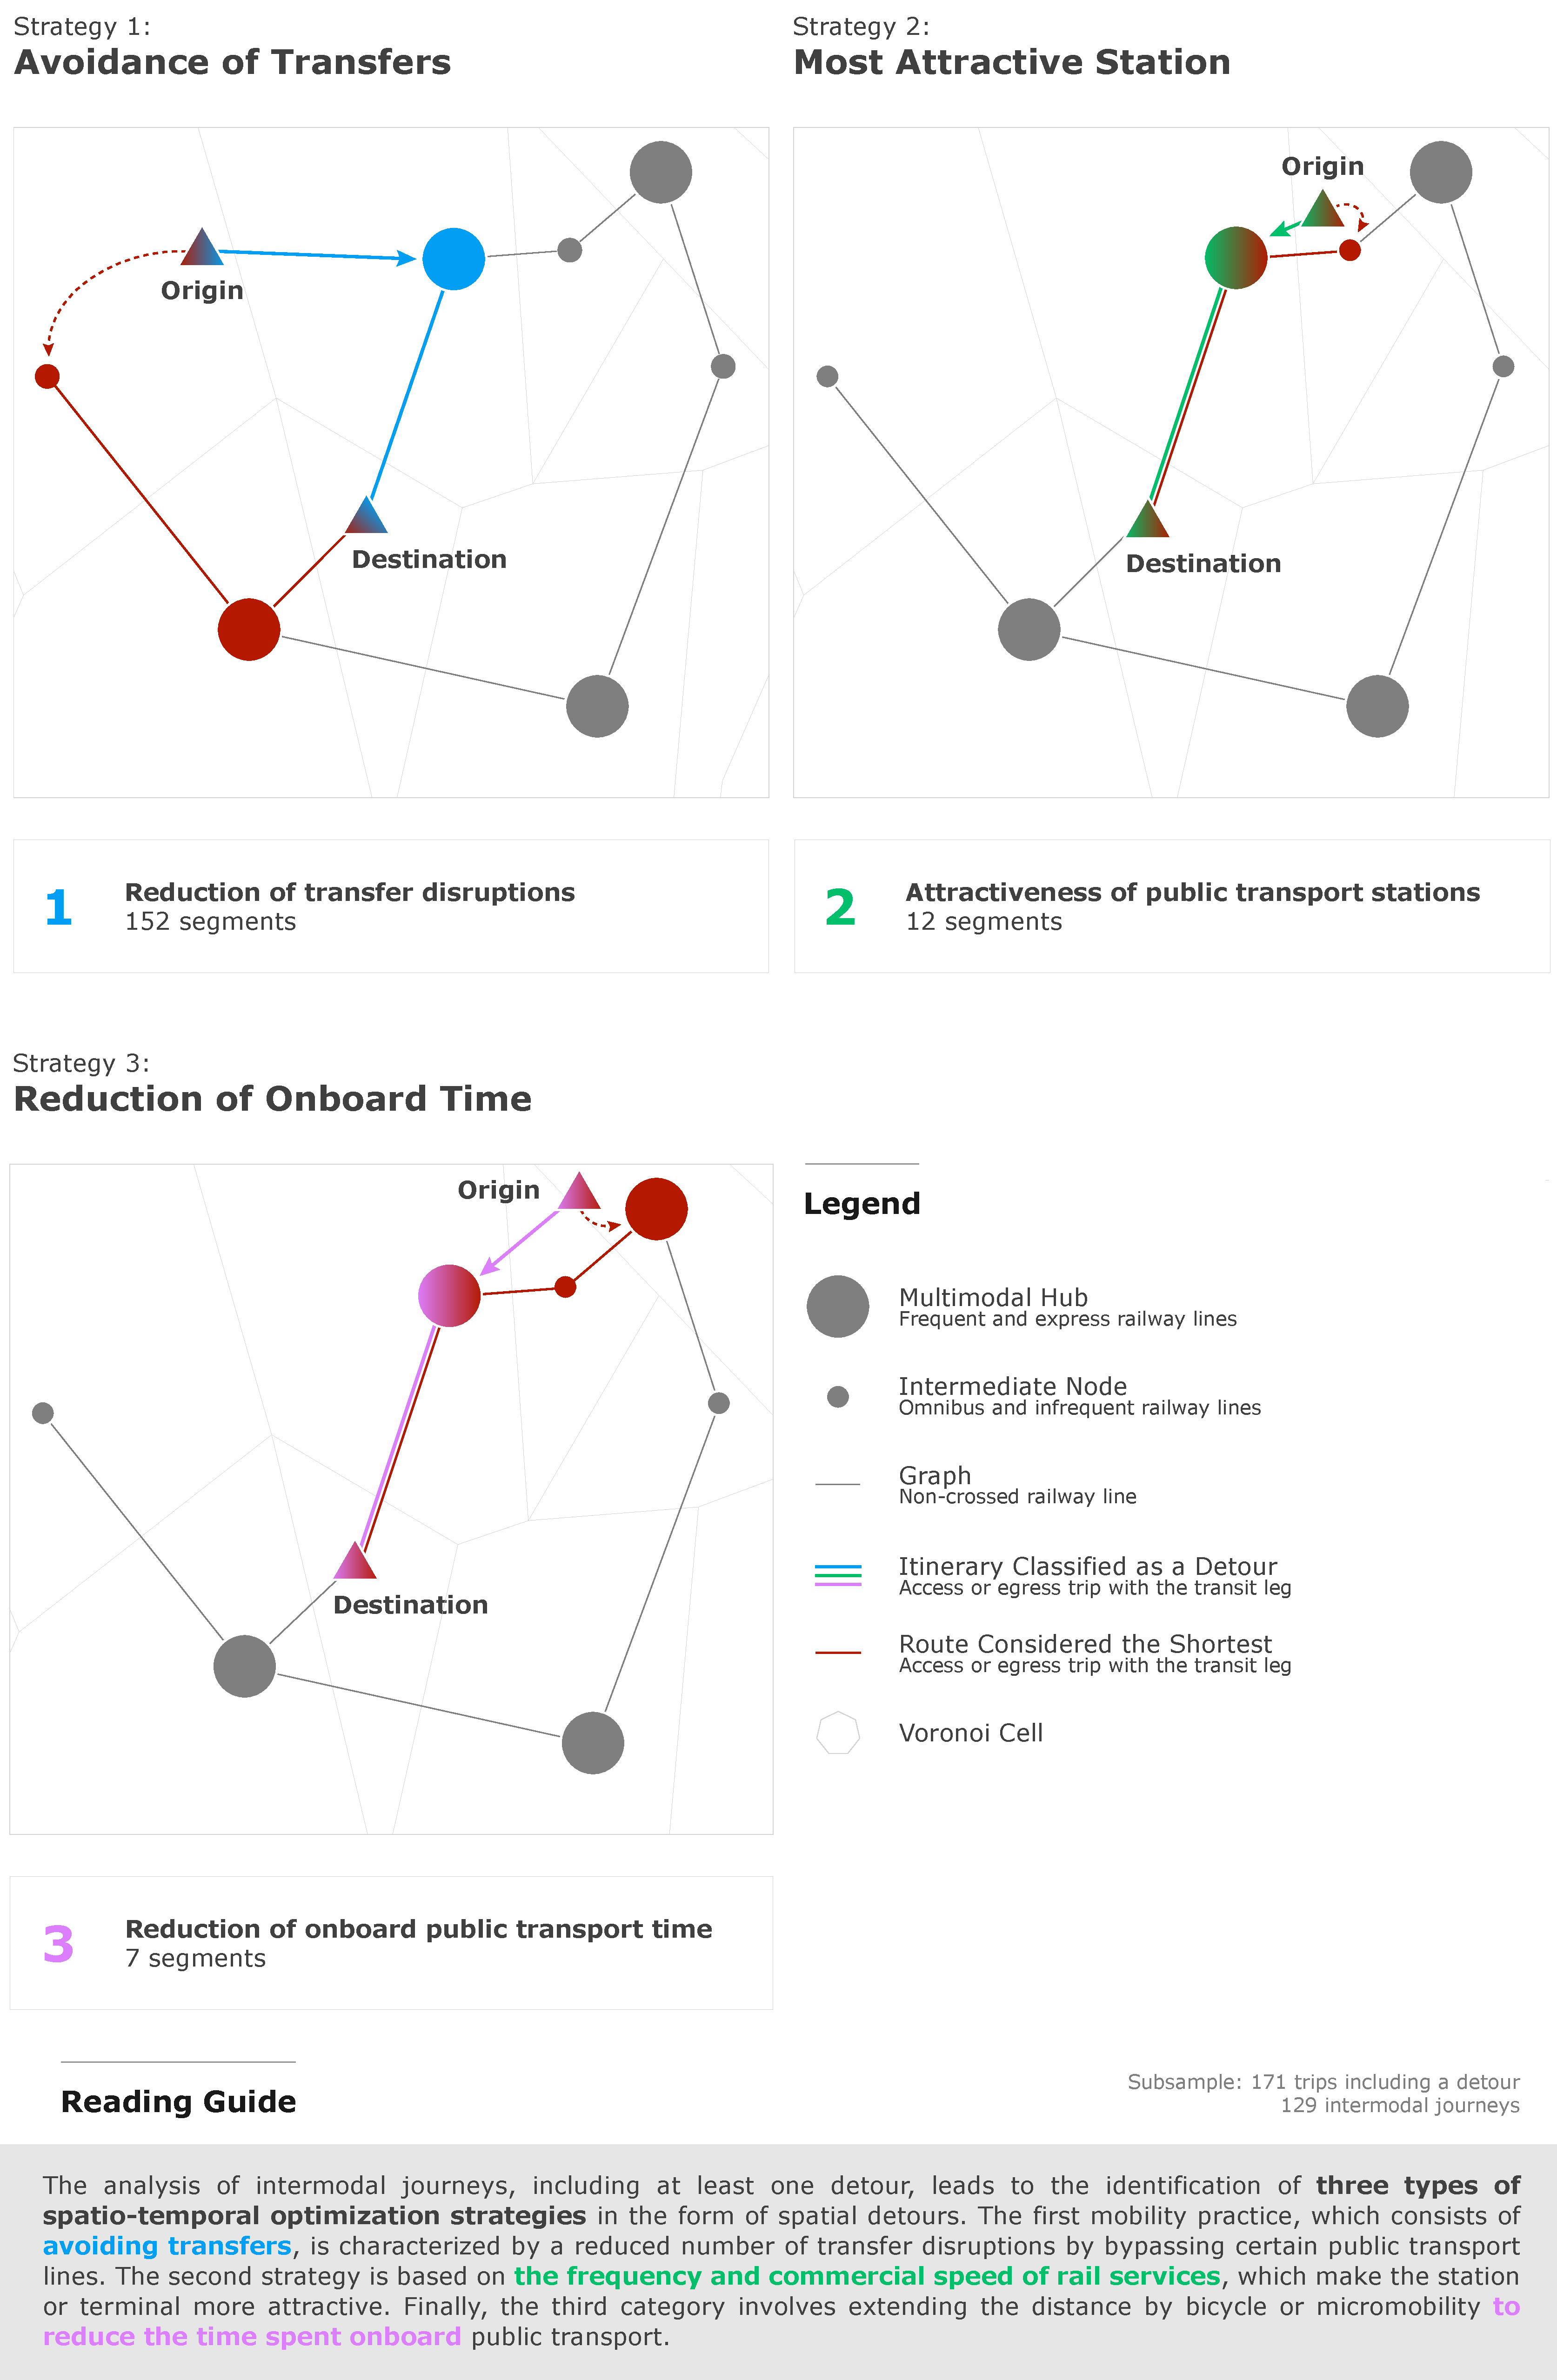
\includegraphics[width=1\columnwidth]{src/Figures/Chap-5/EN_Detours_Typologie.pdf}}
        \caption{Classification of optimization strategies incorporating detours within intermodal trips.}
        \label{fig-chap5:classification-strategies-optimisation-detours}
        \vspace{5pt}
        \begin{flushright}\scriptsize{
        Author: \textcolor{blue}{Dylan Moinse (2023)}
        }\end{flushright}
    \end{carte}

% Classification method
The development of this typology of detours is based on several characteristics of the \acrshort{E-TVS} trips analyzed in \Marque{QGIS}. The variables examined include the actual distances and times traveled by bike or micromobility and by public transport, the total number of transfers during the trip, the frequency of each mode of transport used, as well as the waiting time associated with transfers. The first strategy identified, \Commas{avoidance of transfers,} applies when the actual trip involves fewer transfers than the alternative trip. The category related to \Commas{more attractive public transport stations} refers to situations where the user favors a public transport station with a higher frequency or one that provides access to a faster system in terms of commercial speed. Finally, the last strategy, corresponding to \Commas{reduction of time spent on public transport,} is chosen when the objective time spent in the public transport network is reduced at the expense of the distance-time traveled by bike or micromobility. It is important to note that this typology considers the scale of each trip made using these light modes of transport to identify the segment on which these three detour-based optimization strategies are implemented.%%Translated%%

% Typology description
The three optimization strategies defined based on the detours observed in this study are characterized as follows:
\begin{enumerate}
    \item The \Commas{avoidance of transfers} strategy is based on the desire to bypass a public transport line by accessing a more distant station in order to avoid one or more transfers. This mobility practice also reduces the waiting times associated with transfers, which are often perceived negatively. This choice also allows the traveler to avoid paying for urban transport. On average, this first strategy results in a trip, either accessing or egressing, that is nine minutes longer for cyclists wishing to avoid a transfer. The strategy aimed at reducing transfer times at the cost of increasing the total travel time aligns with the weighting used in transport econometrics concerning these durations, which are perceived very negatively by travelers. This optimization strategy was identified in 152 of the 171 segments in access and egress. In half of the cases, these detours correspond to the avoidance of a metro line;
    \item The strategy of favoring a \Commas{more attractive public transport station} is based on the preference for a station offering a better service level (\textsl{Level of Service}, LOS) compared to the station closest to the origin or destination, without reducing the number of transfers. In most observed situations, this mobility practice allows not only a higher frequency of trains but also faster trains. This optimization strategy was identified in twelve access and egress trips;
    \item The strategy aimed at \Commas{reducing time spent on public transport} involves accessing a more distant public transport station, yet one that offers the same quality of service as the closest station, in order to reduce the time spent on public transport. Only seven trips were classified under this detour-based optimization strategy.
\end{enumerate}%%Translated%%

% Discussion of the typology of detours
This typology of detours taken by intermodal travelers supports several contributions found in the scientific literature. In The Hague, \textcolor{blue}{\textcite[3]{rijsman_walking_2019}}\index{Rijsman, Lotte|pagebf}\index{Molin, Eric|pagebf}\index{Teijl, Thomas|pagebf}\index{Oort, Niels van|pagebf}\index{Ton, Danique|pagebf}\index{Hoogendoorn, Serge|pagebf} indeed concluded that the reasons behind choosing a more distant public transport stop by pedestrians are primarily related to the desire to avoid a transfer, and to a lesser extent to the quality and comfort of the transport service. At the same time, \textcolor{blue}{\textcite[468]{jonkeren_bicycle-train_2021}}\index{Jonkeren, Olaf|pagebf}\index{Kager, Roland|pagebf}\index{Harms, Lucas|pagebf}\index{te Brömmelstroet, Marco|pagebf} and \textcolor{blue}{\textcite[2144]{krizek_bicycling_2010}}\index{Krizek, Kevin~J.|pagebf}\index{Stonebraker, Eric~W.|pagebf} highlight the role of the most attractive and comfortable transport stations in the Netherlands. Our geostatistical analysis also reveals an additional measured time of nine minutes for the first optimization strategy, based on the avoidance of transfers, in accordance with the literature on this topic. The Dutch study by \textcolor{blue}{\textcite[665]{mil_insights_2020}}\index{Mil, Joeri~F.P. van|pagebf}\index{Leferink, Tessa~S.|pagebf}\index{Annema, Jan Anne|pagebf}\index{Oort, Niels van|pagebf} highlights a preference for an additional five to ten minutes by bike to reduce the number of transfers. Furthermore, \textcolor{blue}{\textcite[143]{kampen_bicycle_2021}}\index{Kampen, Jullian van|pagebf}\index{Knapen, Luk|pagebf}\index{Pauwels, Eric|pagebf}\index{Mei, Rob van der|pagebf}\index{Dugundji, Elenna~R.|pagebf} and \textcolor{blue}{\textcite{kampen_understanding_2021}}\index{Kampen, Jullian van|pagebf}\index{Jayaraj, Manoj Ashvin|pagebf}\index{Pauwels, Eric|pagebf}\index{Mei, Rob van der|pagebf}\index{Dugundji, Elenna~R.|pagebf} demonstrate that intermodal cyclists in the Greater Amsterdam area prefer to head to the second nearest station if the train journey is shorter or to avoid a transfer, especially among travelers under 39 years old with a net monthly income below~\euro2,500. Moreover, these insights could resonate with other types of trips not included in this doctoral research, such as \Commas{undirected trips,} which contribute to increased personal satisfaction, as evidenced by the work of \textcolor{blue}{\textcite[8-9]{hook_undirected_2021}}\index{Hook, Hannah|pagebf}\index{Vos, Jonas de|pagebf}\index{Acker, Veronique van|pagebf}\index{Witlox, Frank|pagebf} on walks in Flanders, Belgium, which tend to be longer and are positively correlated with well-being, particularly since they require more physical activity.%%Translated%%

% Typology of pauses
A second aspect related to optimization strategies lies in the \gls{break} that necessarily occurs during mode transfers, particularly when entering and exiting a public transport system, in the case of intermodal trips. This intermediate time related to waiting for public transport can be seen as an opportunity to optimize the travel chain, but also as a chance to engage in additional activities during the trip. The 110 respondents who reported having engaged in an activity during their waiting time at the station were asked to specify the types of activities they favored, using a multiple-choice question followed by an open-ended response. The analysis of spatiotemporal optimization through breaks shows that the majority of breaks were used as an opportunity to make purchases, while a quarter of the respondents stated that they took advantage of the break times to engage in social interactions or professional activities (see \hyperref[table-chap5:motifs-pauses]{Table~\ref{table-chap5:motifs-pauses}}, page~\pageref{table-chap5:motifs-pauses}). More specifically, travelers primarily indicated that the secondary reason related to purchases was mainly food-related, while reasons related to social encounters and professional activities were mainly driven by accompanying children and productive time related to work.%%Translated%%

    % Tableau Typologie pauses
% Pause Typology Table
%%Translated%%
        \begin{table}[h!]
        \centering
        \renewcommand{\arraystretch}{1.5}
        \resizebox{\columnwidth}{!}{
        \begin{tabular}{p{0.58\columnwidth}p{0.21\columnwidth}p{0.21\columnwidth}}
        %\hline
    \rule{0pt}{15pt} \textcolor{blue}{\textbf{Break Typology}} & \textcolor{blue}{\textbf{Count}} & \textcolor{blue}{\textbf{Share}}\\
        \hline
\small{Purchases} & \small{82} & \small{74.5\%} \\
\small{Social meetings and accompaniment} & \small{30} & \small{27.3\%} \\
\small{Professional activities} & \small{27} & \small{24.5\%} \\
\small{Leisure} & \small{23} & \small{20.9\%} \\
\small{Administrative tasks} & \small{17} & \small{15.5\%} \\
\small{Visits and walks} & \small{16} & \small{14.5\%} \\
        \hline
        \end{tabular}}
    \caption{Reasons for the 110 breaks reported by intermodal cyclists during intermodal journeys.}
    \label{table-chap5:motifs-pauses}
        \vspace{5pt}
        \begin{flushleft}\scriptsize{
        \textcolor{blue}{Note:} As the question allowed multiple choices, the total share exceeds 100\%.
        \\
        \textcolor{blue}{Reading Guide:} Purchases are the primary reason for breaks during intermodal trips, followed by social meetings and accompaniment, and professional activities. This table highlights the diversity of reasons associated with trip interruptions.
        }\end{flushleft}
        \begin{flushright}\scriptsize{
        Author: \textcolor{blue}{Dylan Moinse (2023)}
        }\end{flushright}
        \end{table}%%Rédigé%%

%% Commented routes
The observations drawn from this statistical analysis align with the practices reported by the participant designated as \(PCTE_{1}\), interviewed during a trip involving both the use of an electric scooter and the \acrshort{TER}. This user shared her experience regarding some of her food shopping practices, typically done on her return trip home, particularly at Lille Flandres station, which serves as her reverse arrival point. She mentions frequently stopping at this station to take advantage of the amenities and commercial services available within this multimodal hub, including, for example, a bakery (see \hyperref[fig-chap5:pcte1a-commerces-lille-flandres]{Figure~\ref{fig-chap5:pcte1a-commerces-lille-flandres}}, page~\pageref{fig-chap5:pcte1a-commerces-lille-flandres}). However, she raises a concern regarding bringing her scooter into commercial spaces. When suggested that a free, dedicated parking space for \acrshort{ePMD} be established at the stations, the participant expressed conditional interest, depending on the context and the nature of her purchases: \Commas{It all depends on the type of purchase. If it's to spend time, but if it's just to buy a baguette, I won’t use it. Because the time to park the scooter and juggle with the subscription cards\dots If I need to visit two or three stores, why not} [10:36, \(PCTE^{TC}_{1}\)].%%Translated%%

%% Figure 2 Commented route PCTE1A
    \begin{figure}[h!]\vspace*{4pt}
        \caption{Image extracted from the filmed route on the folding path towards Lille Flandres station, showing the station with some commercial services (\(PCTE^{A}_{1}\)).}
        \label{fig-chap5:pcte1a-commerces-lille-flandres}
        \centerline{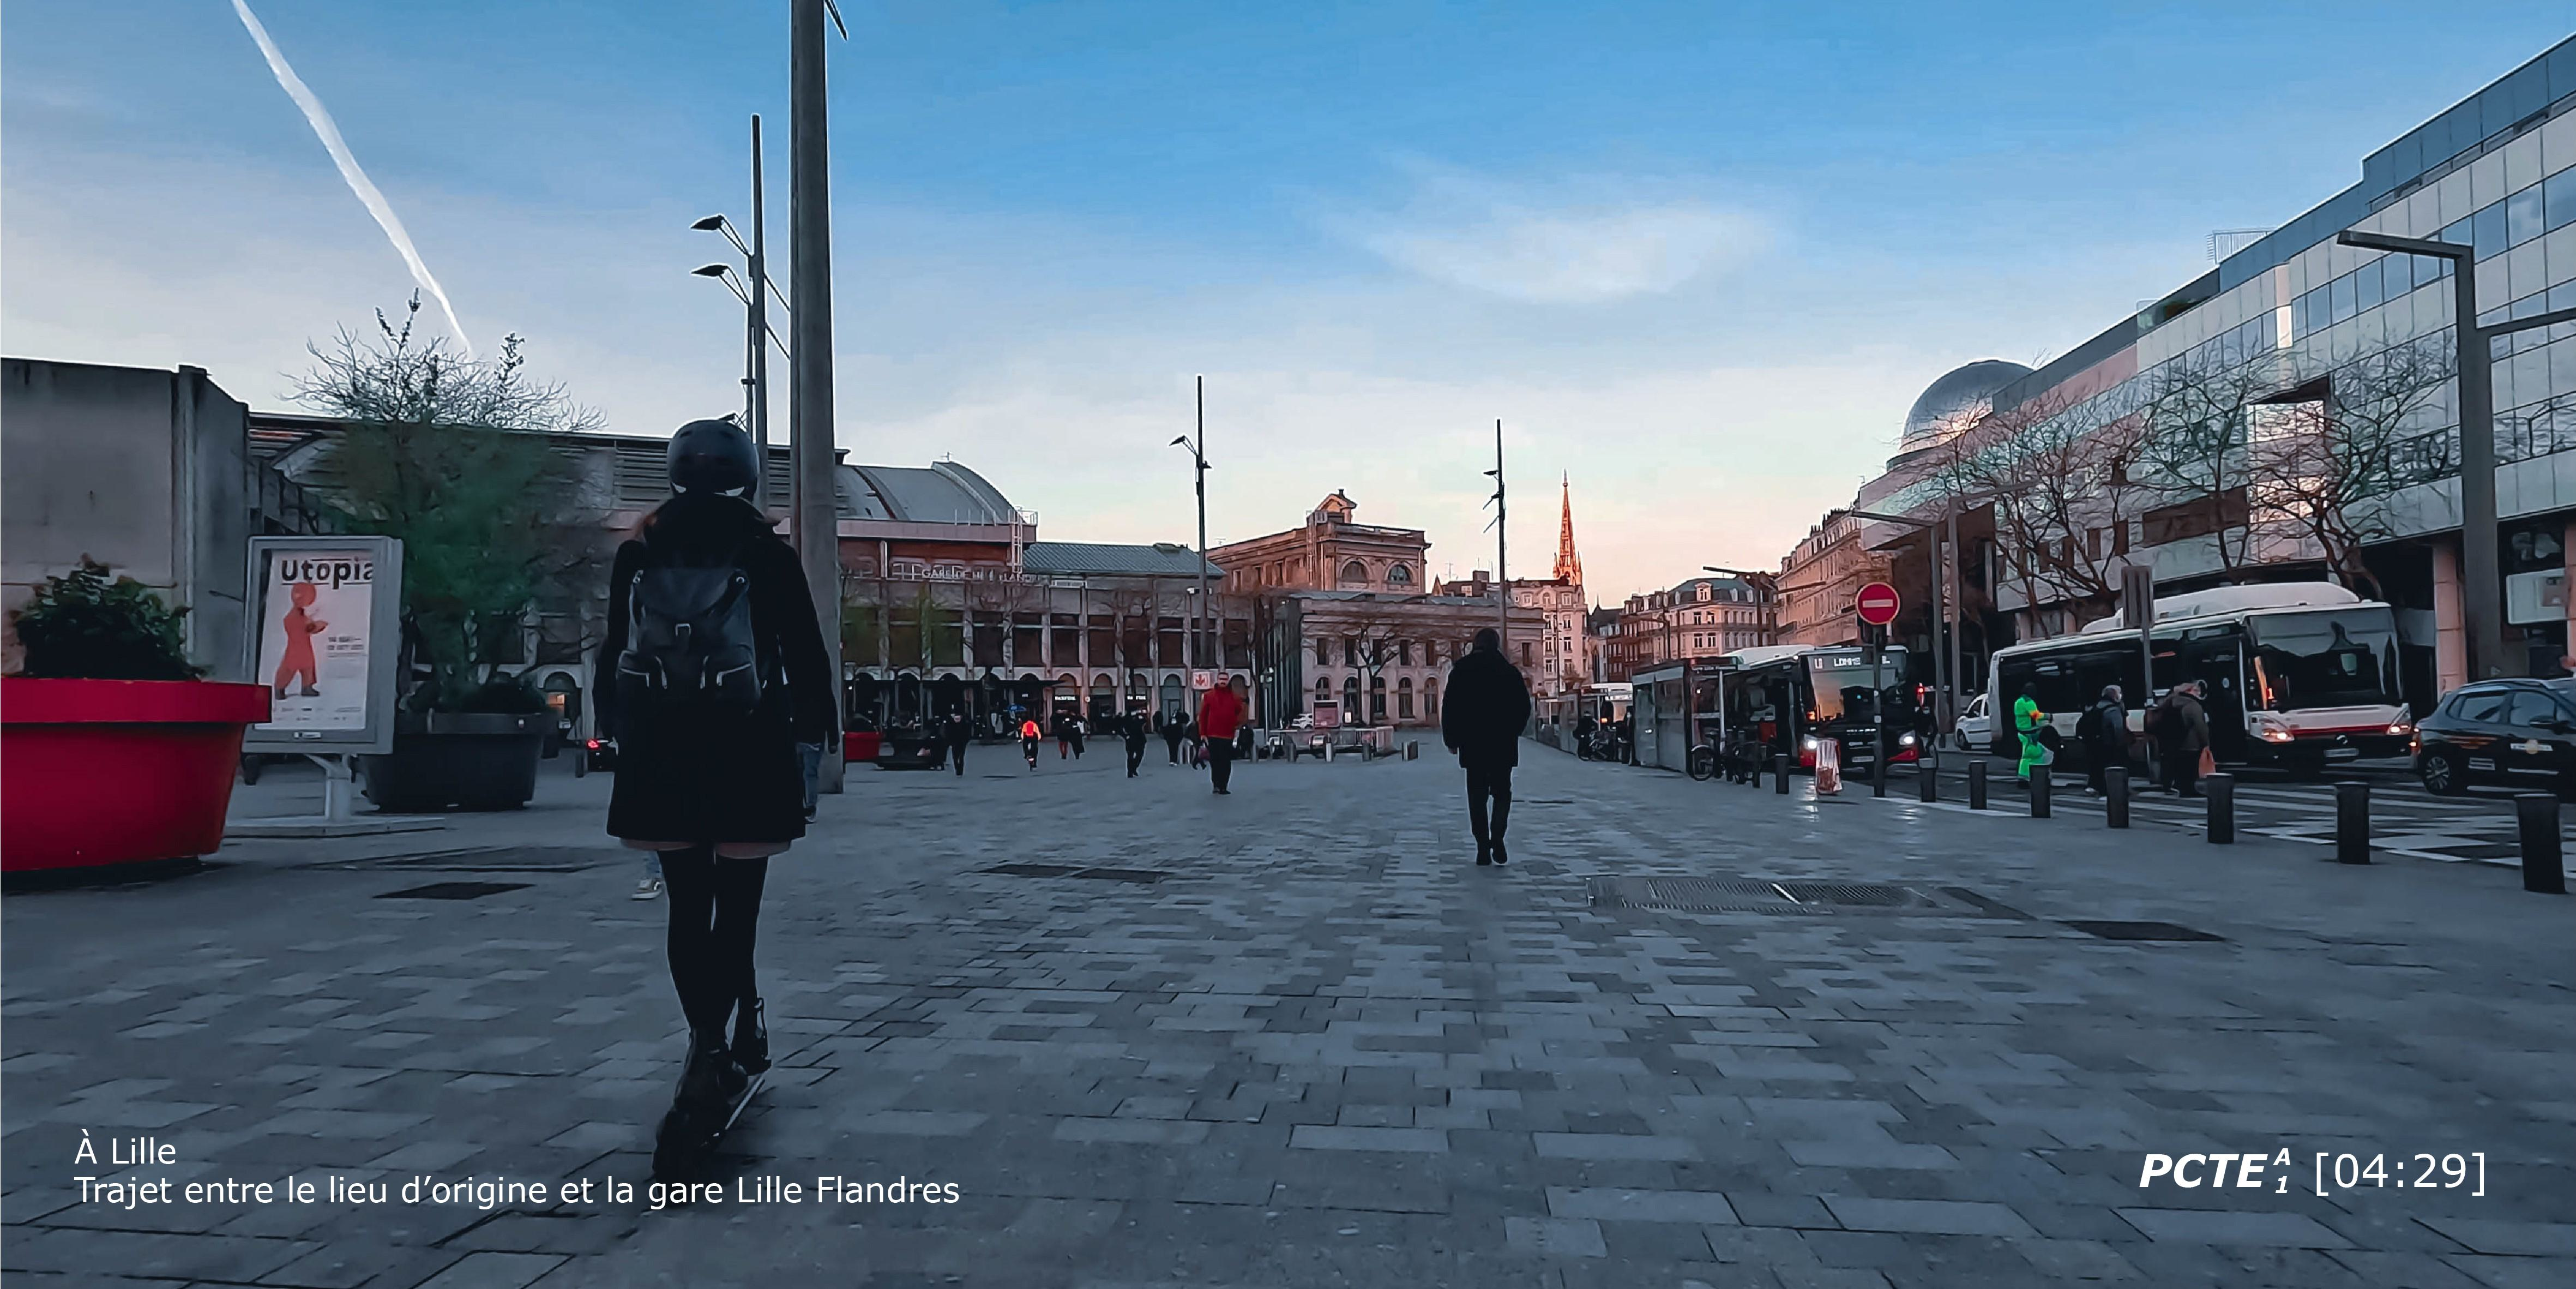
\includegraphics[width=1\columnwidth]{src/Figures/Chap-5/EN_Detours_PCTE1_Access_13.jpg}}
        \vspace{5pt}
        \begin{flushright}\scriptsize{
        Author: \textcolor{blue}{Dylan Moinse (2022)}
        }\end{flushright}
    \end{figure}
  
% Discussion of equipped time
The concept of time spent on trips has undergone a significant evolution in contemporary research, particularly regarding its use in public transport. Previously perceived mostly as a constraint or disutility, the time spent in transport is now seen by some economists as an opportunity for optimization and the enhancement of daily activities. This reassessment fits within a perspective where travel time is no longer viewed solely as a loss, but as a resource that can be used productively. According to the work of \textcolor{blue}{\textcite[28]{joly_rapports_2003}}\index{Joly, Iragaël|pagebf}, this valuation is part of a broader search for space and comfort, leading individuals to accept a time investment in transport. Individual strategies for optimizing time spent on public transport, studied by \textcolor{blue}{\textcite[85]{jain_gift_2008}}\index{Jain, Juliet|pagebf}\index{Lyons, Glenn|pagebf}, reflect a desire to make this time useful, whether through professional activities or leisure. In this view, passive modes of transport, such as public transport, become spaces in which certain productivity is exercised \textcolor{blue}{\autocite[115]{lyons_use_2007}}\index{Lyons, Glenn|pagebf}\index{Jain, Juliet|pagebf}\index{Holley, David|pagebf}. Travel time is then used for various activities, from work to leisure such as reading or listening to music, thus contributing to well-being and personal fulfillment \textcolor{blue}{\autocite[17]{moinse_temps_2020}}\index{Moinse, Dylan|pagebf}. However, the valuation of this time depends on various factors such as comfort, ergonomics, accessibility, network knowledge, and even connectivity to communication networks \textcolor{blue}{\autocite[21]{bounie_what_2019}}\index{Bounie, Nathan|pagebf}\index{Adoue, François|pagebf}\index{Koning, Martin|pagebf}\index{L'Hostis, Alain|pagebf}. \Commas{Equipped time} \textcolor{blue}{\autocite[87]{jain_gift_2008}}\index{Jain, Juliet|pagebf}\index{Lyons, Glenn|pagebf}, illustrates a competitive advantage of public transport systems by offering time for various activities, not only for commuting but also for leisure trips \textcolor{blue}{\autocite[111]{lyons_use_2007}}\index{Lyons, Glenn|pagebf}\index{Jain, Juliet|pagebf}\index{Holley, David|pagebf}. In this context, emerging mobilities such as autonomous cars present a challenge for public transport. By offering autonomy similar to that of public transport, these new forms of mobility could undermine its competitiveness. Furthermore, this phenomenon could create a paradox with the promotion of active mobility, as \Commas{equipped time} encourages less active modes of transport\footnote{~
    \textcolor{blue}{\textcite[21]{bounie_what_2019}}\index{Bounie, Nathan|pagebf}\index{Adoue, François|pagebf}\index{Koning, Martin|pagebf}\index{L'Hostis, Alain|pagebf} measured, using an ordinal logit model, the effects of smartphone use and mobile connectivity on the reduction of spatiotemporal constraints encountered aboard the Paris metro. Their analysis demonstrated that the perceived value of travel time decreases by 12\% when users have access to mobile networks during their trip.
}.%%Translated%%

% Discussion of pauses
The possibility of engaging in these activities largely depends on the availability of break time and activity and service sites located in or near the railway station. This analysis highlights the positive role of breaks in intermodal trips, emphasizing the contribution of urban amenities to the formation of optimal distances and, consequently, optimal trips, within the broader goal of promoting alternatives to cars for regional mobility. This connection between transport issues and urban development calls for renewed attention from urban and transport stakeholders regarding the design of railway stations and their surroundings, as well as the distribution of services. This aligns with the study conducted by \textcolor{blue}{\textcite[468]{jonkeren_bicycle_2021}}\index{Jonkeren, Olaf|pagebf}\index{Kager, Roland|pagebf}, which shows that visiting supermarkets and other stores is the most frequent activity for chaining trips on the cycling access portion.%%Translated%%

% 5.3.3.5.
\needspace{1\baselineskip} % Reserve space
\subsubsection*{Clustering of Intermodal Detour-based Journeys from the Perspective of Spatiotemporal Optimization
    \label{chap5:clusterisation-detours}
    }

% Type of analysis
By estimating the different optimization ratios (\(R\)), the statistical analysis aims to group intermodal trips based on the measured distance gains. To do this, we compared the spatial optimization coefficient (\(R_{km}\)) and the perceived temporal optimization coefficient (\(R_{t_{(P)}}\)) in order to categorize the routes according to the two variables used. On one hand, the spatial optimization ratio refers to the spatial distance gains made by comparing the actual spatial distance (\(km_{eff}\)) with the shortest possible spatial distance, referred to as the alternative (\(km_{alt}\)). On the other hand, the temporal optimization ratio represents the time gains made between the perceived and actual travel time (\(t_{eff_{(P)}}\)) and the alternative time (\(t_{alt_{(P)}}\)). Based on the values obtained for \(R_{km}\) and \(R_{t_{(P)}}\), this statistical evaluation positions the analyzed \acrshort{E-TVS} trips in relation to spatial and temporal balances. In this way, the analysis is presented in the form of a bubble chart representing \(R_{t_{(P)}}\) as a function of \(R_{km}\) (see \hyperref[fig-chap5:profils-strategies-optimisation-detours]{Figure~\ref{fig-chap5:profils-strategies-optimisation-detours}}, page~\pageref{fig-chap5:profils-strategies-optimisation-detours}). A third variable is also displayed in the statistical reading, which is based on the difference between the spatial distance of actual trips (\(km_{eff}\)) and that of alternative trips (\(km_{alt}\)), while a final categorical variable indicates the type of optimization strategy involved. It should be noted that this clustering analysis method relies on the concept of visual grouping, that is, the detection of point concentrations based on a graph crossing various variables, and does not rely on algorithms designed to establish advanced grouping. Instead, this approach represents a preliminary analysis of the types of intermodal cyclists who opt for detours.%%Translated%%

%% Figure clustering of detour profiles
    \begin{figure}[h!]\vspace*{4pt}
        \caption{Grouping of intermodal trips involving a detour according to spatiotemporal optimization profiles.}
        \label{fig-chap5:profils-strategies-optimisation-detours}
        \centerline{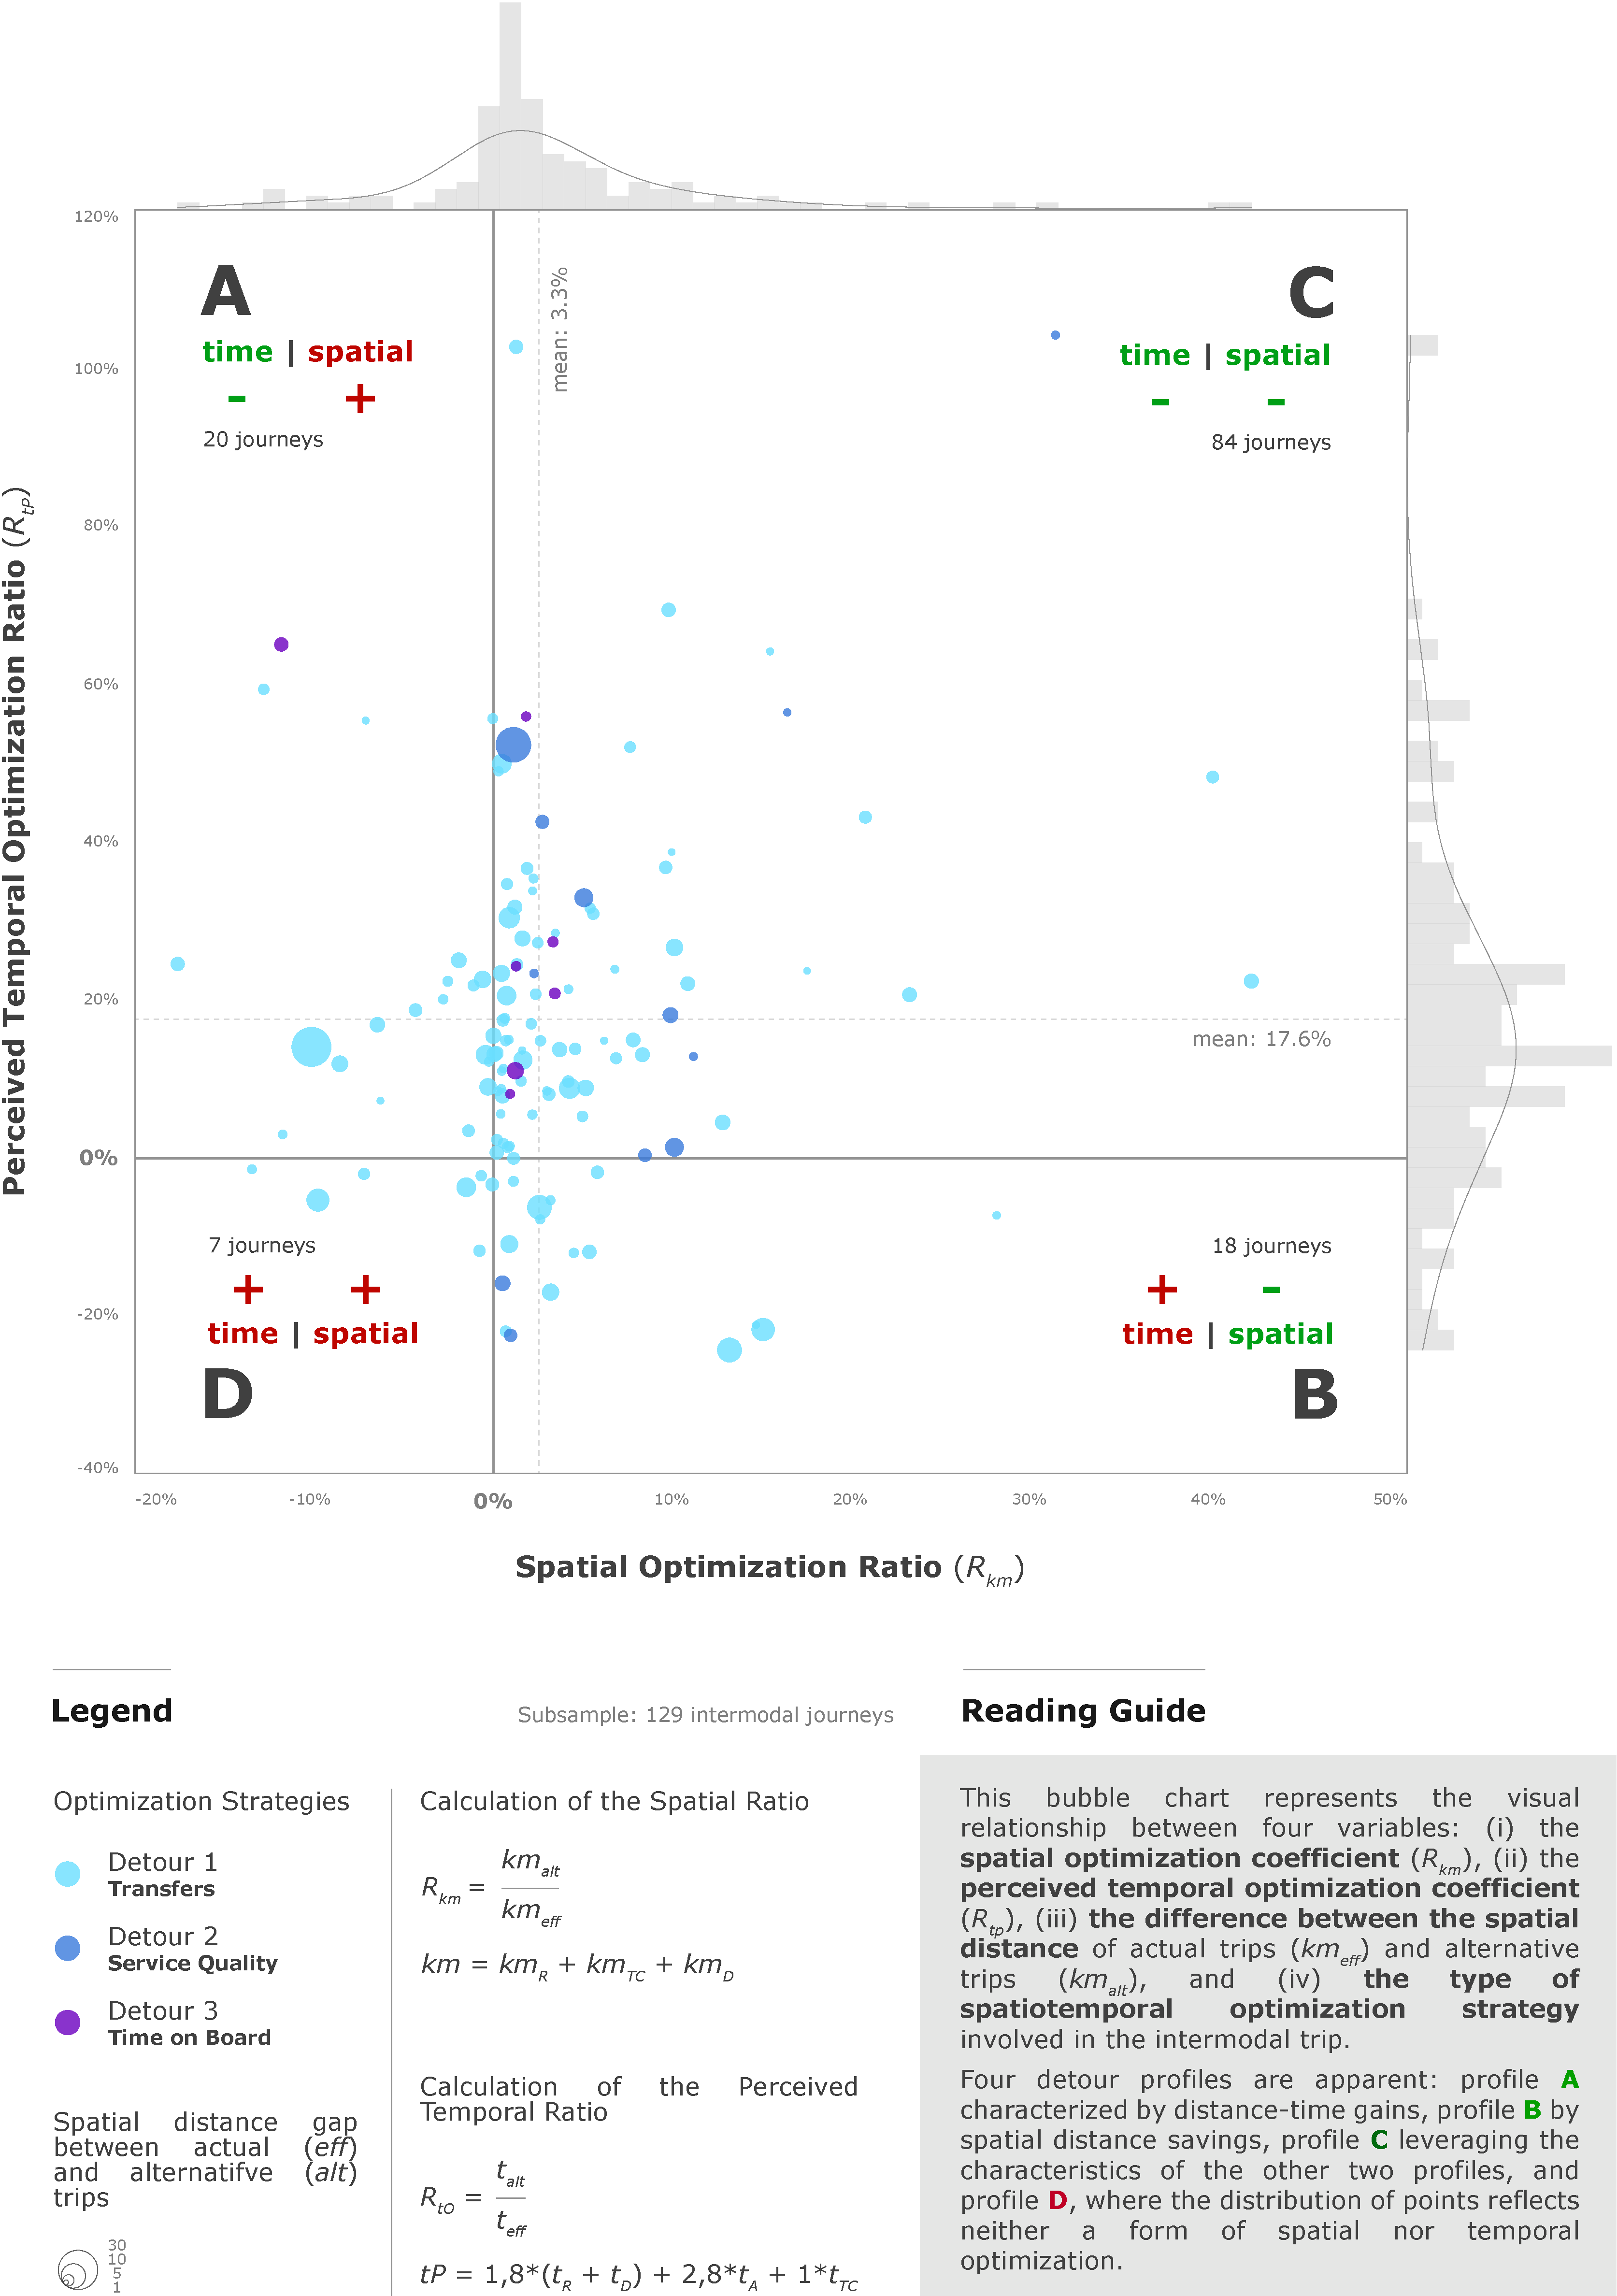
\includegraphics[width=1\columnwidth]{src/Figures/Chap-5/EN_Detours_Cluster_optimisation_detours.pdf}}
        \vspace{5pt}
        \begin{flushright}\scriptsize{
        Author: \textcolor{blue}{Dylan Moinse (2023)}
        %\\
        %Created with \Marque{Python}~and \Marque{Illustrator}
        }\end{flushright}
    \end{figure}
    
    % Results
The statistical analysis through the clustering of \acrshort{E-TVS} trips aims to better understand the role of detours in the search for spatiotemporal optimization. This approach highlights four detour profiles that generate optimization. Profile \(A\) is characterized by distance-time savings but an unfavorable spatial distance ratio, whereas profile \(B\) favors spatial distance gains at the expense of distance-time. Meanwhile, profile \(C\) combines advantages in both distance-time and spatial terms, while profile \(D\) exhibits a negative spatial and temporal optimization ratio. The graphical representation, as shown in \hyperref[fig-chap5:profils-strategies-optimisation-detours]{Figure~\ref{fig-chap5:profils-strategies-optimisation-detours}} (page~\pageref{fig-chap5:profils-strategies-optimisation-detours}), reveals a dense clustering of 84 \acrshort{E-TVS} trips (65\%) within profile \(C\). Additionally, by combining profiles \(A\), \(B\), and \(C\), we observe that 95\% of the analyzed routes are included. This result suggests that almost all of the studied detours provide savings in distance-time and/or spatial distance compared to alternative routes. On the other hand, the spatial difference between actual and alternative routes does not seem to have a simple effect on the spatiotemporal optimization ratios, implying that a small detour can, under certain conditions, significantly optimize an intermodal trip.%%Translated%%

    % Transition
However, the examination of certain detours within profile \(D\), for which spatiotemporal optimization is not demonstrated, suggests that exogenous factors, which are neither spatial nor temporal, could justify the choice of such routes.%%Translated%%

% 5.3.4.
\needspace{1\baselineskip} % Reserve space
\subsection{Crossed Perspectives on Detours, Breaks, and Optimization
    \label{chap5:discussion-detours-pauses-optimisation}
    }

% Introduction
Although this research has deliberately focused on distance-related dimensions, it remains essential to incorporate fundamental variables influencing route choices within mobility behaviors, such as the characteristics of the urban environment, network configurations, as well as the ambiance and stress levels associated with intermodal practices that include the use of bicycles and micromobility \textcolor{blue}{\autocite[79]{zuo_incorporating_2021}}\index{Zuo, Ting|pagebf}\index{Wei, Heng|pagebf}\index{Chen, Na|pagebf}.%%Translated%%

% 5.3.4.1.
\needspace{1\baselineskip} % Reserve space
\subsubsection*{Influence of Public Space Valuation on Optimization Strategies
    \label{chap5:environnement-urbain}
    }

% Role of the urban environment (ID 145 Houchin to Loos-lez-Lille)
Considering the role played by the urban environment, particularly the treatment of public spaces and its impact on modal choice as presented in the \acrfull{SLR} of \hyperref[chap2:titre]{Chapter~2} (page~\pageref{chap2:titre}), we chose to adopt a qualitative approach based on a case study from the administered questionnaire. This example of declared intermodal travel was selected in relation to the geographical context in which it takes place. The spatial analysis of this journey, characterized by a spatiotemporal optimization strategy including detours, indeed involves the \acrshort{CABBALR} and the \acrshort{MEL}. The intermodal trip investigated is thus made on the conventional railway network between Béthune station and Lille CHR stop, with an origin located in Houchin, about four kilometers from Béthune station as the crow flies, and a destination in Loos-lez-Lille, about two kilometers from the stop. Taken at least five times a week, this trip involves the use of a personal car to the first regional station, then the train and \acrshort{PeS} from the intermediate station. It is noteworthy that the respondent's home is closer to Nœux-les-Mines station (3 kilometers as the crow flies) and the destination is closer to Loos-lez-Lille station (0.4 kilometers), as depicted on \hyperref[fig-chap5:exemple-detours-lille-chr]{Map~\ref{fig-chap5:exemple-detours-lille-chr}} (page~\pageref{fig-chap5:exemple-detours-lille-chr}). Nevertheless, the detours made both in access and egress provide this traveler with a way to optimize their journey.%%Translated%%

% Diversion
Within the first segment of the journey to Béthune station, we can observe a strategy aimed at reducing the constraint associated with a transfer. Although the railway line connecting Béthune and Lille CHR stations is direct, via the K50 or C50 trains linking Saint-Pol-sur-Ternoise to Lille\footnote{~
    \textcolor{blue}{\textcite[468]{sncf_voyageurs_trains_nodate}} refers to the various \acrshort{TER} lines implemented based on the type of service and the train's commercial speed: the \acrshort{TER} of the \Commas{KRONO} (\(K\)) type ensures direct connections with few stops between regional hubs, the \acrshort{TER} of the \Commas{CITI} (\(C\)) type ensures medium-distance connections around cities, while the \acrshort{TER} of the \Commas{PROXI} (\(P\)) type ensures local connections. It should be noted that this classification may vary depending on the services and regions.
}, the journey from Nœux-les-Mines station to Lille requires a transfer at Béthune. Initially, the traveler should take, from Nœux-les-Mines station, the K52 line linking Arras to Dunkirk or P54 between Arras and Calais-ville to Béthune, or these same lines in the reverse direction towards Lens. Secondly, the traveler should switch to the K50 or C50 line between Saint-Pol-sur-Ternoise and Lille from Béthune station or the K51 or C51 line between Lens and Lille. However, by traveling an additional five minutes by personal car during the access phase, the traveler can directly reach Béthune station from their starting point in Houchin. Indeed, the access journey theoretically lasts fifteen minutes instead of ten minutes, not considering urban congestion effects, but this traveler gains a notable distance-time advantage in public transport, as well as avoiding a transfer and, consequently, an additional waiting time. This distance-time gain is even more significant during off-peak hours, when the frequency of trains is considerably reduced—even though this trip is excluded from the quantitative analysis of detours since it was made by car—with waiting times that can extend from 1.5 to 2 hours between the two \acrshort{TER}. Thus, this first detour, which is part of the strategy we have termed \Commas{transfer avoidance,} allows for a minimum saving of fifteen minutes during peak hours, even considering the additional five minutes of car travel, and up to over an hour during off-peak hours.%%Translated%%

% Figure example detour Loos vs Lille CHR
    \begin{carte}[h!]\vspace*{4pt}
        \caption{The structuring presence of a bicycle lane along an egress itinerary, made by personal electric scooter and taking the form of a detour from Lille CHR stop.}
        \label{fig-chap5:exemple-detours-lille-chr}
        \centerline{\includegraphics[width=1\columnwidth]{src/Figures/Chap-5/EN_Detours_Carte_Exemple_Lille_CHR.png}}
        \vspace{5pt}
        \begin{flushright}\scriptsize{
        Author (A): \textcolor{blue}{Dylan Moinse (2024)} with data from \textcolor{blue}{\textcite{openstreetmap_openstreetmap_2023}}
        \\
        Sources (B): Images of rue Frédéric Combemale, in Lille, from \Marque{Google Street View} dated July 2019
        \\
        Photography of rue Frédéric Combemale, in Lille (C): \textcolor{blue}{Dylan Moinse (2023)}
        }\end{flushright}
    \end{carte}
    
% Diversion
Regarding the egress journey, the intermodal traveler makes a second detour by using a \acrshort{PeS}, favoring the Lille CHR stop over Loos-lez-Lille station. This choice can be explained by a search for spatiotemporal optimization adapted to the railway offer. Indeed, the K50 and K51 lines allow reaching this public transport hub in 25 to 31 minutes. In contrast, Loos-lez-Lille station, served only by the local C50 and C51 lines, requires between 41 and 45 minutes of travel. The distance between Lille CHR stop and the destination is seven minutes, compared to three minutes from the closest station to Loos-lez-Lille, so the journey by \acrshort{PeS} is extended by a four-minute detour. This detour results in a time gain estimated between 6 and 16 minutes, with the additional advantage of a doubled frequency, providing access to the K50, K51, as well as C50 and C51 lines. Consequently, such an egress detour fits into the second optimization strategy called \Commas{more attractive public transport stations.} While the access journey is characterized by a relatively direct path to Béthune station, it is also important to note that the egress journey is marked by the presence of a spatial inversion. Thus, this intermodal trip, characterized by two types of detours and a pronounced spatial inversion, optimizes the movement by providing a distance-time gain of 21 to 41 minutes during peak hours and at least one hour during off-peak hours. On a weekly scale, these optimization strategies through detours allow for significant time savings due to the pendular nature of this journey, made twice a day, five days a week. The traveler thus falls into profile \(A\), showing a willingness to increase spatial distance for a gain in distance-time.%%Translated%%

% Bicycle lanes
The last aspect discussed in this subsection concerns the influence of the urban environment in relation to detours within the travel chain. The quality of public spaces and urban forms can be the main reasons for adopting detours and a complex modal combination involving the use of the car, \acrshort{TER}, and \acrshort{PeS}. The use of a personal car for access raises questions, hence our interest in this specific case study. It should be noted that the car journey between Houchin and Béthune takes place on a departmental road (D72), with the 500 meters crossed in the municipality of Houchin being developed as a \acrfull{CVCB}\footnote{~
    The \acrshort{CVCB}, also known as \Commas{chaucidou}, is a type of road without an axial marking where the shoulder lines are close to its axis, aiming to redistribute road space for the benefit of cyclists by ground markings. Motor vehicles circulate on a bidirectional central lane, and cyclists use the paved shoulders called \Commas{rives.} When motor vehicles cross paths, drivers must use the shoulders, resulting in less comfortable conditions than dedicated bike lanes \textcolor{blue}{\autocite[24]{jouannot_mieux_2018}}\index{Jouannot, Thomas|pagebf}. The observational and questionnaire survey conducted by \textcolor{blue}{\textcite[21]{cerema_nord_picardie_chaussee_2018}} on the \acrshort{CVCB} of Boulevard de Strasbourg in Saint-Omer shows a marked improvement in cyclist safety, even in the presence of heavy motor traffic. However, this three-lane setup should only be proposed when the constraints are such that no other solution is feasible \textcolor{blue}{\autocite[27]{jouannot_mieux_2018}}\index{Jouannot, Thomas|pagebf}.
}~inaugurated in 2022 and accompanied by a speed limit of 30 km/h. The rest of the departmental road, which extends over about three kilometers, more than half of the hypothetical route, is marked by a classic setup of two car lanes with heavy motor traffic and a speed limit of 50 km/h, previously 80 km/h. Apart from the \Commas{chaucidou} at the start of the municipality of Houchin and the pedestrian bridge at Béthune station, the access route is entirely shared among different modes of transport. In contrast, the egress journey made by \acrshort{PeS} is characterized by a recent bicycle lane directly connecting the Lille CHR stop to Loos-lez-Lille station, likely used by the cyclist, assuming they chose the shortest path. The construction of this bike lane near the Lille CHR stop was inaugurated during the reopening of Frédéric Combemale and Jacques Malbernat streets in Lille on June 4, 2022 (see \hyperref[fig-chap5:exemple-detours-lille-chr]{Map~\ref{fig-chap5:exemple-detours-lille-chr}}, page~\pageref{fig-chap5:exemple-detours-lille-chr}). Thus, just under half (0.9 km) of the egress route, which is 2 kilometers long and likely used by the commuter, is marked by the presence of a bike lane serving the secondary entrance of Lille CHR station, though it is relatively unknown to intermodal cyclists according to visual recordings from our quantitative observation. The other half of the egress route is only crossed by one-way streets, with low motor traffic and a speed limit of 30 km/h. We can therefore hypothesize that a lower quality bike lane, combined with a longer distance, partly explains the choice of the car for access.%%Translated%%

% Car VS TEP
Another question concerns the competitiveness of this modal choice compared to the exclusive use of the car between the origin and destination points. A car-only journey takes 60 minutes, excluding congestion, using the shortest route via a motorway (A21) and national roads (N47 and N41), which are often saturated towards the Lille metropolitan area. In comparison, the intermodal journey made by the traveler takes, \textsl{a priori}, between 47 and 53 minutes. Not taking into account parking time and traffic jams on one hand, and the precautionary time usually estimated at five or ten minutes and potential disruptions in the railway network on the other, the intermodal journey seems competitive compared to driving. This also justifies the choice of \acrshort{PeS} rather than walking combined with urban public transport. Indeed, if we consider a bus journey (line 82) from Houchin to Béthune station, the access typically takes 30 minutes, while the walk from Lille CHR stop to the destination takes over 25 minutes.%%Translated%%

% 5.3.4.2.
\needspace{1\baselineskip} % Reserve space
\subsubsection*{Influence of Temporality on Optimization Strategies
    \label{chap5:temporalite}
    }

% Introduction performance index
This case study has shown that the mobility practice of connecting to distant railway hubs generates distance-time gains and allows individuals to benefit from a better quality of service, provided that cycling infrastructure is available. In this last subsection, we aim to address the concept of accessibility through the lens of temporality. The central question is to examine the distance-time gains measured in relation to the temporal opportunities offered at the destination. Beyond travel time, the challenge is to evaluate the performance of the public transport system integrating the use of light individual mobility.%%Translated%%

% Figure performance detours Noeux-les-Mines
    \begin{figure}[h!]\vspace*{4pt}
        \caption{Evaluation of the performance of intermodal chains, involving the use of light individual mobility, applied around Noeux-les-Mines station.}
        \label{fig-chap5:performance-detours-noeux}
        \centerline{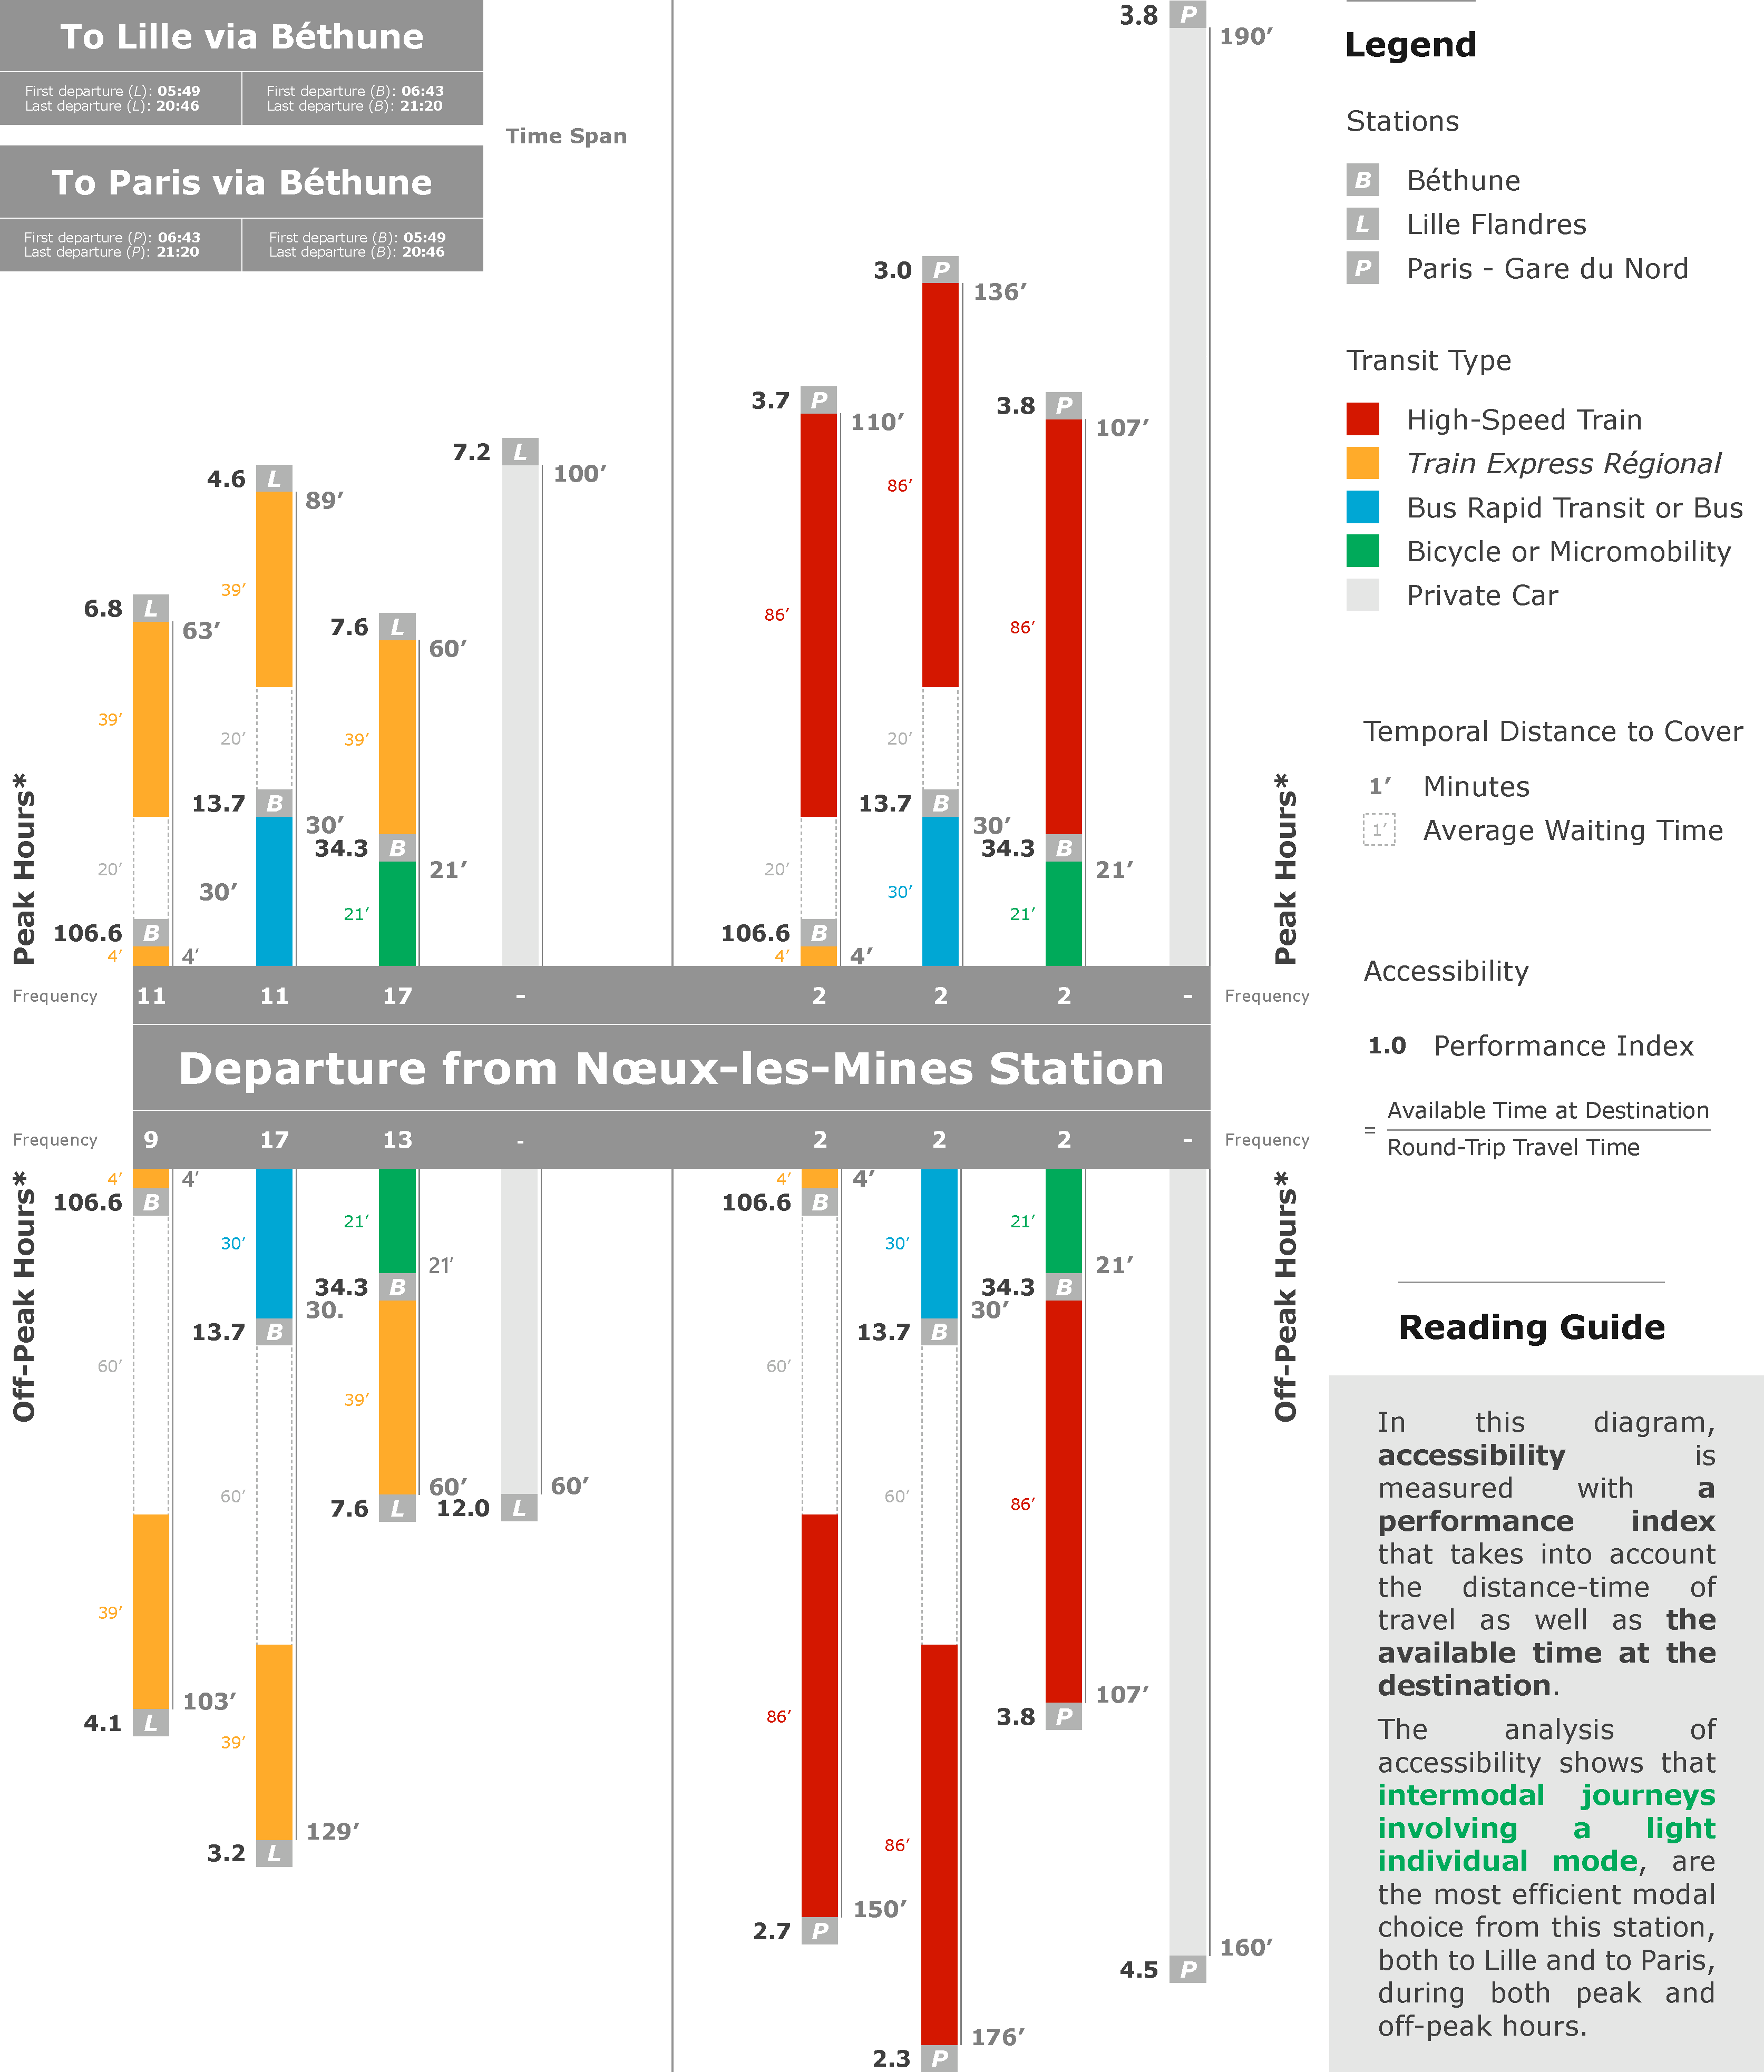
\includegraphics[width=1\columnwidth]{src/Figures/Chap-5/EN_Detours_Performance_Noeux_les_Mines.pdf}}
        \vspace{5pt}
        \begin{flushleft}\scriptsize{
        \textcolor{blue}{Note:} peak hours correspond to the time interval between 6:30 AM and 9:30 AM and between 4:30 PM and 7:30 PM on weekdays. Conversely, off-peak hours extend from 7:30 PM to 6:30 AM and 9:30 AM to 4:30 PM on weekdays.
        }\end{flushleft}
        \begin{flushright}\scriptsize{
        Sources: \acrshort{GTFS} from January 27, 2024, to April 26, 2024, sourced from \textsl{Open Data} of \textcolor{blue}{\textcite{sncf_sncf_2022}}
        \\
        Author: \textcolor{blue}{Dylan Moinse (2024)}
        }\end{flushright}
    \end{figure}
 
% Existing literature
In the spirit of space-time geography, referring to the \textsl{Time Geography} movement, this subsection focuses on applying an indicator based on the ability to perform a daily activity, taking into account individual temporal rhythms. This temporal perspective was primarily adopted by Swedish geographer \textcolor{blue}{Gunnar} \textcolor{blue}{\textcite{tornqvist_contact_1984}}\index{Törnqvist, Gunnar|pagebf}, who developed a method to measure the potential for establishing direct contacts, called \Commas{contact potential}\footnote{~
    This approach, centered on the diffusion of innovation in relation to regional development and the growing specialization of activities, involves an increase in the number of contacts between individuals.
}. As emphasized by \textcolor{blue}{\textcite[9-11]{lhostis_contribution_2018}}\index{L'Hostis, Alain|pagebf}\index{Liu, Liu|pagebf}\index{Leysens, Thomas|pagebf}, this indicator initially integrated the available duration at the destination, distance-time, and the cost of a daily round-trip journey by different modes of transport. It aimed to illustrate the existing connections in space between locations. Empirically, these \Commas{opportunities for face-to-face contacts}, based on the relationship between the maximum duration of stay and the size of each urban population, were first explored in 98 urban centers by \textcolor{blue}{\textcite[13, 18]{tornqvist_contact_1984}}\index{Törnqvist, Gunnar|pagebf}, who established a linear relationship between the demographic size of the metropolitan area and the need for contact. \textcolor{blue}{\textcite[12]{lhostis_contribution_2018}}\index{L'Hostis, Alain|pagebf}\index{Liu, Liu|pagebf}\index{Leysens, Thomas|pagebf} note that the handling of transfers and intermodality are crucial aspects of measuring distance-time, which are only adequately addressed from a time-scheduling perspective. Hence, the importance of adopting a time-based approach to constructing monomodal and intermodal routes. Contact potential, or \textsl{contactability} \textcolor{blue}{\autocite[]{haggett_geography_2001}}\index{Haggett, Peter|pagebf}, thus allows the analysis of relationships between cities and transport, as studied by \textcolor{blue}{\textcite[6]{lhostis_using_2017}}\index{L'Hostis, Alain|pagebf}\index{Liu, Liu|pagebf}\index{Leysens, Thomas|pagebf} from the perspective of the impact of the new high-speed rail line between Tours and Bordeaux.%%Translated%%

% Case study Noeux-les-Mines: time gains
Building on our previous case study, our analysis focuses on the station closest to the user's home, namely Noeux-les-Mines station, towards the flow-generating hubs represented by the Lille and Paris metropolitan areas. By comparing the various travel times as well as the frequency and time span of different modal combinations, we sought to assess the comparative advantages of intermodal travel versus travel solely by public transport or car. As shown in \hyperref[fig-chap5:performance-detours-noeux]{Figure~\ref{fig-chap5:performance-detours-noeux}} (page~\pageref{fig-chap5:performance-detours-noeux}), the intermodal chain, consisting of reaching Béthune station using a bicycle or a micromobility option before taking the train to Lille or Paris, ensures a notable distance-time gain during both peak and off-peak hours. For the example of Noeux-les-Mines station, the total travel time to Lille Flandres station is reduced to 60 minutes using this intermodal practice, compared to 63 minutes using only the \acrshort{TER}, and 107 minutes to Gare du Nord, compared to 110 minutes using the \acrshort{TER} and \acrshort{HST}. During off-peak periods, the time gap increases in favor of intermodal travel involving a detour, with a recorded time gain of 43 minutes for destinations in Lille and Paris. This detour strategy not only leads to a distance-time saving and reduced effort related to transfer disruptions, but also provides access to a better service level in terms of frequency. Indeed, the user combining light individual mobility and the train minimizes their exposure to railway disruptions and thus avoids the inconveniences related to transfers, while gaining direct access to the more frequent Béthune - Lille line. However, this observation is not as evident for the intermodal travel scenario to Gare du Nord, given that only three to four \acrshort{HST} trains serve Béthune station on weekdays. Despite this, and aside from the time saving, the choice to travel directly to Béthune station for Paris allows the individual to avoid poorly synchronized transfers between the \acrshort{TER} and the \acrshort{HST}, with connection times of less than five minutes.%%Translated%%

% Case study Noeux-les-Mines: performance index
The case study on accessibility around Noeux-les-Mines station leads us to evaluate the effectiveness of the synergy between light individual mobility and the railway network from a temporal perspective. Our approach, based on a scenario in which the individual wishes to travel to Lille or Paris from this public transport hub, reveals that the choice of an intermodal trip marked by a detour also allows for better temporal opportunities at the destination. Inspired by \Commas{the overall performance index}\footnote{~
The performance index involves comparing the maximum duration of stay and the round-trip travel time \textcolor{blue}{\autocite[]{cauvin_accessibilite_1989}}\index{Cauvin-Reymond, Colette|pagebf}\index{Reymond, Henri|pagebf}\index{Schaub, Gérard|pagebf}, in order to consider the difficulty of obtaining the available minute at the destination and thus measure the effectiveness of the railway offer in a given context \textcolor{blue}{\autocite[130]{chapelon_transports_2016}}\index{Chapelon, Laurent|pagebf}. Through our case study, the performance index developed from Noeux-les-Mines station is based on a weekday, outside of educational break periods, specifically Monday, January 29, 2024.
} measured by \textcolor{blue}{Laurent} \textcolor{blue}{\textcite[130]{chapelon_transports_2016}}\index{Chapelon, Laurent|pagebf} in his study on available time in Paris around the \acrshort{HST} network, our analysis highlights the temporal efficiency offered by intermodal travel. By combining the use of a bicycle or micromobility with the \acrshort{TER} towards Lille, the performance index reaches 7.6, compared to 6.8 during peak hours and 4.1 during off-peak hours for monomodal train travel. Similarly, the ratio for Paris is 3.8, compared to 3.7 during peak hours and 2.7 during off-peak hours. This reading, based on temporal opportunities at the destination, demonstrates how integrating light individual mobility with rail transport can enhance the accessibility of a location (see \hyperref[fig-chap5:performance-detours-noeux]{Figure~\ref{fig-chap5:performance-detours-noeux}}, page~\pageref{fig-chap5:performance-detours-noeux}). Conversely, a monomodal journey by bicycle or micromobility to Béthune station is not competitive compared to the exclusive use of the \acrshort{TER}, both in terms of the required distance-time and the ratio of available time on-site. It is worth noting that with the \acrfull{SERM} project, which will serve Béthune and Lille Flandres stations, the effectiveness of the modal combination involving light individual mobility from Noeux-les-Mines station will be much more significant and could, with significantly improved frequency and time span, make this type of route more competitive than driving. However, this case study reveals certain dysfunctions in the public transport system that tend to reduce its attractiveness: although the efficiency of intermodal travel is higher during peak hours, the car proves more efficient during off-peak periods due to a reduced time span.%%Translated%%

% 5.3.4.3.
\needspace{1\baselineskip} % Reserve space
\subsubsection*{Influence of Socio-demographic Characteristics on Optimization Strategies
    \label{chap5:sociodemographie}
    }

% Role of demographics
Considering the socio-demographic characteristics of the sub-sample obtained relating to intermodal travelers who adopted detour and break strategies, it is important to note that these intermodal travelers have a gender and age distribution similar to that of train users in France: 39\% of these travelers are women, while 60\% are between 25 and 45 years old, with only 12\% under 25. However, these users relying on \acrshort{E-TVS} journeys tend to be more often full-time professionals or students (85\%).%%Translated%%

% Modal combination
Regarding their modal combination, 69\% of commuters who integrated detours or breaks into their journeys primarily favor the use of the \acrshort{TER}, and up to 91\% when using all interurban public transport systems. On the light individual mobility side, 47\% of trips involving detours or breaks were made by personal bicycle, 19\% by \acrshort{PeS}, 12\% by folding bike, and 9\% by \acrshort{PBS}. This distribution within the studied sub-sample does not exactly reflect the modal distribution of transfer modes as observed by the research firm \textcolor{blue}{\textcite{enov_enquete_2021}}\index{Enov@\textsl{Enov}|pagebf} and by \textcolor{blue}{\textcite[180]{moinse_intermodal_2022}}\index{Moinse, Dylan|pagebf}\index{Goudeau, Matthieu|pagebf}\index{L'Hostis, Alain|pagebf}\index{Leysens, Thomas|pagebf}, who reported an equal modal share between conventional bicycles and \acrshort{PeS} for transfers to the train in France.%%Translated%%

% ___________________________________________
% 5.*.
\newpage
\needspace{1\baselineskip} % Reserve space
\addcontentsline{toc}{section}{Conclusion of Chapter~5}
\sectionheader{Conclusion of Chapter~5}
\section*{Conclusion of Chapter~5
    \label{chap5:conclusion}
    }
    \markright{Conclusion of Chapter~5}{} 

% Synthesis
This chapter, focused on distances, routes, and more generally, on accessibility, has highlighted the comparative advantages of the intermodal use of light individual mobility. On one hand, the analysis of the distances traveled by users reveals an extension of the train station neighborhoods at the local scale, thereby renewing the delineation of strategic areas specific to \acrshort{TOD}. This comparison of cycling paths led us to examine how bicycles and micromobility leverage their extended range to make intermodal travel more competitive. This is reflected not only in facilitating access to public transport networks but also in optimizing travel. On the other hand, by adopting a regional perspective, we were able to assess the effects of accessibility gains on demographic coverage and the service of destinations.%%Translated%%

% 5.*.*
\needspace{1\baselineskip} % Reserve space
\subsection*{Main Findings
    \label{chap5:principaux-enseignements}
    }

% Local distances
As part of our first research objective focused on expanding train station neighborhoods based on the different types of vehicles specific to light individual mobility and the factors influencing the distances traveled, it was established that the spatial distance considered acceptable for pendular flows is 3.8 kilometers on each side of the intermodal journey. The relevant range for this set of transport modes is between 0.8 and 4.2 kilometers for the feeder stage, and between 0.5 and 3.3 kilometers for the egress stage. Walking proves more competitive below these thresholds, while urban public transport and cars are more competitive beyond them.%%Translated%%

% Influence of transport types
These distances also vary depending on the type of public transport system used, with modal combinations including the use of the \acrshort{HST} recording an acceptable distance of four kilometers, compared to three kilometers for the \acrshort{TER} and two kilometers for the metro and tram. The quality of the service level offered by stations also influences these distances, with stations offering the best services having an acceptable distance of 4.8 kilometers, compared to 4.3 kilometers for those offering average service and 3.8 kilometers for the least attractive ones.%%Translated%%

% Influence of other factors
Other factors exert a positive influence on the distance traveled, such as frequency of use and \acrshort{PCS} favoring senior executives, as well as the number of individuals in a household and modal substitution from cars for the access segment. This corresponds to an average travel duration of twelve minutes for light individual mobility as a transfer mode. It was also observed that the same mode of transport is used for the first and last kilometers by more than 83\% of folding bike users and 79\% of \acrshort{PeS} users, indicating that vehicles best suited for boarding collective modes meet a specific need related to the egress phase.%%Translated%%

% Size of train station neighborhoods
As a result, the delineation of pedestrian train station neighborhoods is 2.6 times larger for combined walking and 22.6 times larger for light individual mobility, compared to the commonly accepted influence areas. At the scale of the overall journey, the median distance for an intermodal trip was identified as 36 kilometers, or 53 minutes, with an acceptable distance of 71 kilometers. Light individual mobility thus accounts for one-fifth of the spatial distance, but more than two-thirds of the distance-time spent.%%Translated%%

% Regional accessibility
The extension of train station neighborhoods thus allows coverage of 22\% of the region as the crow flies and 8\% of the territory based on the road network. In response to our second objective, focused on regional accessibility gains, we identified an improvement in the population accessibility rate, reaching 56\% of residents. This means serving three times more individuals around the stations compared to the areas accessible by foot, and in territories that are four times less densely populated. The integration of light individual mobility into the railway network significantly improves the coverage of the regional population and offers increased potential for more inclusive mobility, reaching housing estates with 2.4 times more social housing, as well as residential areas where the median property value is 9.5\% lower than in pedestrian train station neighborhoods. Our analysis of the geographic distribution of households based on available income also highlighted a median income 3.6\% higher, but with less pronounced gaps between the lower and upper quartiles.%%Translated%%

% Accessibility of jobs
Our study of real estate transactions concerning spaces dedicated to industrial, commercial, and office sectors has shown that more distant train station neighborhoods remain attractive, with median transaction values 5\% higher. This dynamic positively influences access to jobs, facilitating access to over 71\% of the job market, representing a 1.76 times increase in the number of accessible jobs. Furthermore, access to \acrshort{POIs} is multiplied by 2.16, allowing potential access to 66\% of the available facilities in the region. More specifically, 79\% of \Commas{premium} category facilities are accessible, compared to 71\% for those in the \Commas{intermediate} range and 62\% for those in the \Commas{proximity} category.%%Translated%%

% Detours and breaks 1
Addressing our final research objective, the identification of routes outside the catchment area of public transport stations and routes punctuated by intermediate stops, led us to reassess the relationships between detours, breaks, and optimization from an intermodal perspective. We concluded that detours, when integrated into pendular trips, can lead to an average time saving of 18\% and a 3\% reduction in spatial distance traveled. In general, commuters deviate from the most direct route, choosing to follow access or egress routes that are three times longer, which results in halving the time spent in public transport and reducing waiting time by 80\%. Another aspect that emerged from this chapter is the grouping of the analyzed trips, which showed that 95\% of the detours examined lead to either distance-time savings or spatial distance reductions, while 65\% of the optimization strategies succeed in achieving both simultaneously.%%Translated%%

% Detours and breaks 2 + Transition
The examination of the distribution of distances shows a significantly larger catchment area for the stations. \acrshort{E-TVS} journeys typically extend from five to six kilometers, which corresponds to a duration of twenty minutes. We can thus deduce that travelers are willing to take an additional two kilometers detour, expanding the service area of stations by 2.3 times and the size of the \Commas{primary area} by 19.9 times. It is demonstrated that the direction taken during intermodal trips influences their efficiency. Time gains are more significant when the detours involve an extreme form of detour, such as a spatial inversion. Moreover, breaks provide an opportunity to make use of waiting times. These interruptions are generally dedicated to daily purchases, fitting into a more complex travel chain. In summary, these two chapters have focused on measuring and explaining the spatial extension of train station neighborhoods induced by light individual mobility, with the aim of assessing the intermodal accessibility gains it enables. Unlike these chapters, which are based on an \Commas{effective accessibility} approach aiming to diagnose actual accessibility conditions, the next part of the doctoral research focuses on \Commas{normative accessibility,} seeking to formulate recommendations to improve accessibility while ensuring their feasibility \textcolor{blue}{\autocite[19]{levine_mobility_2019}}\index{Levine, Jonathan|pagebf}\index{Grengs, Joe|pagebf}\index{Merlin, Louis~A.|pagebf}.%%Translated%%

% ___________________________________________
     \newpage
     
% Valorisation scientifique
    \begin{tcolorbox}[colback=white!5!white,
                      colframe=blue!75!blue,
                      title=Valorization
                      \\
                      Chapter~5]
\Large{\textcolor{blue}{\textbf{Scientific Article:}}}
    \\\\
\small{\textcolor{blue}{\textcite{moinse_optimizing_2024}}\index{Moinse, Dylan|pagebf}\index{L'Hostis, Alain|pagebf}. Optimizing Intermodal Commuting by way of Detours and Breaks: Evidence of Micromobility Users in France. \textsl{Journal of Transport Geography}. 116(103821), (1-16~p.).
\\
\footnotesize{\url{https://doi.org/10/gtkvs9}} (\textbf{ACL})}
    \\\\
\Large{\textcolor{blue}{\textbf{Congress:}}}
    \\\\
\small{\textcolor{blue}{\textcite{moinse_optimizing_2023}}. Optimizing intermodal commuting by way of detours and breaks. Evidence of micromobility users in France. \textsl{World Conference on Transport Research} (WCTR), Montréal. 
\\
\footnotesize{\url{https://hal.science/hal-04166574}} (\textbf{C-ACTI})}
    \\\\
\Large{\textcolor{blue}{\textbf{Seminars:}}}
    \\\\
\small{\textcolor{blue}{\textcite{moinse_eclater_2022}}. Éclater la bulle des périmètres du Transit-Oriented Development (TOD). Vers un Micromobility-based TOD à l'échelle régionale ? \textsl{Rencontres TerriTrans - MoTAU}, Aix-en-Provence. 
\\
\footnotesize{\url{https://hal.science/hal-03881592}} (\textbf{C-COM})}
    \\\\
\small{\textcolor{blue}{\textcite{moinse_analysis_2021}}. An Analysis of Intermodal Use of e-Scooters with train in the Provence-Alpes-Côte d’Azur Region, in France: Towards Extended Railway Station Areas? \textsl{Smart And Sustainable Cities Conference}, \textsl{Urban mobility, New Technologies and Urban Development}, Paris.
\\
\footnotesize{\url{https://shs.hal.science/halshs-03507433}} (\textbf{C-ACTI})}
    \\\\
\small{\textcolor{blue}{\textcite{moinse_analyse_2021}}. Une analyse de l’usage intermodal des trottinettes avec le train dans la région Provence-Alpes-Côte d’Azur. Vers une extension des quartiers de gare? \textsl{Future Days}, Mobilité décarbonée, Paris.
\\
\footnotesize{\url{https://hal.science/hal-03473394}} (\textbf{C-COM})}
    \\\\
\Large{\textcolor{blue}{\textbf{Communications:}}}
    \\\\
\small{\textcolor{blue}{\textcite{moinse_trottinettes_2022}}. \textsl{Des trottinettes pour « éclater la bulle » des transports en commun}, Fête de la Science : Ateliers 1 classe, 1 scientifique, 1 heure, Paris 
\\
\footnotesize{\url{https://shs.hal.science/halshs-03810191}}}
    \\\\
\small{\textcolor{blue}{\textcite{moinse_jpeux_2022}}. J’peux pas prendre le train, j’vis trop loin de la gare pour y aller à pied, \textsl{Revue d'Urbanisme et d'Expression Urbaine lÂme Urbaine}, 12, 15~p.
\\
\footnotesize{\url{https://www.asso-envar.com/la-revue}}}
    \\\\
\small{\textcolor{blue}{\textcite{moinse_temps_2020}}. Le temps dans les transports. Cadeau ou fardeau? \textsl{Revue d'Urbanisme et d'Expression Urbaine lÂme Urbaine}, 11, 17~p.
\\
\footnotesize{\url{https://www.asso-envar.com/la-revue}}}
    \end{tcolorbox}

    % ___________________________________________
    % Subbibliography
    \newpage
    \sectionheader{Bibliography of Chapter~5}
    \begingroup
    \renewcommand{\bibfont}{\scriptsize}
\printbibliography[segment=\therefsegment, heading=subbibintoc, title={Bibliography of Chapter~5}, label=chap5:bibliographie]
    \endgroup
    \end{refsegment}